%\documentclass[journal=jpr,manuscript=article]{achemso}
\documentclass{article}
\usepackage[margin=0.5in]{geometry}
\usepackage{graphicx}
\usepackage{mathtools,amssymb}
\usepackage{dsfont}
\usepackage{color}
\usepackage[english]{babel}
\usepackage{authblk}
\usepackage{url}
%\usepackage{soul}
\usepackage[normalem]{ulem}
%\usepackage[ruled,vlined,linesnumbered]{algorithm2e}
%\usepackage{algorithmic}
\usepackage[colorlinks,citecolor=blue,linkcolor=blue,bookmarks=false,hypertexnames=true, urlcolor=blue]{hyperref} 

%\graphicspath{{figs/}}  Store figures at the level of the main doc
\newcommand{\argmax}{\text{argmax}}
\newcommand{\todo}[2]{{\color{red} {\bf TODO-#1}: #2}}
\newcommand{\comment}[2]{{\color{blue} {\bf Comment-#1}: #2}}
\newcommand{\correction}[2]{{\color{red}\sout{#1}}{\color{red}#2}}
%\newcommand{\correction}[2]{#2}  % Use this to make a document with hiding track changes.
\newcommand{\edit}[1]{{\color{red}#1}}

%\usepackage[backend=biber,style=nature,articletitle=false]{biblatex}
%\usepackage[backend=biber,style=nature]{biblatex}
%\addbibresource{bibliography.bib}

%\usepackage[backend=biber]{biblatex}
%\usepackage{natbib}
%\addbibresource{bibliography.bib}
\newcommand{\pe}[0]{\mathrel{{+}{=}}}
\newcommand{\mathone}{\mathds{1}}

\usepackage{setspace}
%\doublespacing
%\newcommand*{\DOUBLEBLINDREVIEW}{} %Uncomment to hide author information for double-blind peer review


\author{Andrey Borevsky}
\author{Attila Kertesz-Farkas$\ast$}
\affil{Laboratory on AI for Computational Biology, Faculty of Computer Science, HSE University,  11 Pokrovsky Bvld., Moscow 109028, Russian Federation}
%\email{akerteszfarkas@hse.ru}
%\phone{+7 (499) 152-07-41}

\title{Toward reliable false discovery rate control in classification problems under distribution shift}
\begin{document}

\maketitle

\begin{abstract}
	Domain shifts or batch effects can significantly degrade the performance of machine learning-based classifiers in software production without any warning. This can particularly be problematic in medical applications which involve human lives. The shift changes the shape of the prediction score distribution of the test samples compared to that of the training samples; hence, decision boundary re-calibration would be required to conform to the expected performance standards. We present a simple, yet robust heuristic method to mitigate the bias in false discovery rate (FDR) control originating from data shifts. Our method is based on an adjustment of the test prediction scores so that the test null distribution (approximated distribution of the prediction scores of negative test samples) aligns to the training null distribution (actual distribution of prediction scores of the negative training samples). We termed it the Test Null Adjustment (TNA) method. Then, accurate empirical p-values of the adjusted test prediction scores can be calculated with respect to the training null distribution to be used in the Benjamini-Hochberg (BH) protocol for FDR control. The main advantage of the TNA method is that its application does not require any domain specific knowledge. It works with multi-class scenario, it is fully data-driven, and it operates in the 1-dimensional space of the prediction scores ensuring stable numerical calculations. We have performed four experimental tests on the biomedical image analysis domain to demonstrate that the TNA method is able to mitigate the bias in FDR induced by data shift in real-life applications. 


\end{abstract}
\textbf{Key words:} Empirical P-values, False Discovery Rate, Data Shift, Batch Effect

\section{Introduction}

Modern AI applications not only need to increase their discriminative power to reduce the overall number of incorrect predictions, but also to simultaneously minimize a quantified risks of false positive (FP) and negative (FN) error by an optimal decision threshold calibration while also being able to handle (or detect) data distribution shift \cite{feng2022clinical, al2023artificial}. False positive (type I) and false negative (type II) errors can have significantly different costs or impacts on people and society \cite{wynants2019three}. For instance, a false positive HIV, COVID-19 or cancer diagnosis can cause emotional trauma and the person may undergo invasive treatments with undesirable complications and side effects \cite{newman2021rate, salz2010meta, Tosteson2014Consequences, xu2016frequency} until a more elaborated clinical test establishes the correct diagnosis. However, a failure to diagnose an infectious disease may lead to a false sense of safety \cite{mouliou2021false}, and may put not only their but other peoples' lives in danger \cite{woloshin2020false}. An undetected cancer may either prolong or hinder treatment \cite{bradley2021interpreting}, and misdiagnosed human papillomavirus (HPV) may progress to cancer precursor lesions \cite{macios2022false,pinsky2015principles}. 


False discovery rate (FDR) control procedures are plausible techniques to keep the FP rate among the total positive classifications at a certain, user-defined level \cite{Benjamini1995Controlling}, when the risk of FP prediction is significantly higher than the cost of FN predictions. FDR control became popular with the emergence of high-throughput and shotgun experiments which measured large numbers of distinct variables simultaneously per sample in a cost efficient way. For instance, automatic patch clamp systems employ a deep-learning-based image processing module to automatically detect target cells (e.g. nerve cells in living brain). Then it calibrates the movement of a micropipette to approach the cell for future experiments \cite{koos2021automatic}. Cell morphological profiling in high-throughput imaging assays for studying compound libraries and human diseases \cite{moshkov2024learning} relies on automatic cell segmentation and detection often in 3D images \cite{falk2019u}. The FDR control here could curb the error in selecting wrong cells for subsequent experiments and feature quantification.  Microarrays measure the expression levels of thousands of genes simultaneously and the FDR control allows the selection of promising genes for followup studies \cite{storey2002direct,storey2003statistical,barber2015controlling}. Tandem mass spectrometry can be used to quantify and identify thousands of proteins in a complex biological/chemical sample and FDR control makes it possible to choose the most trustworthy protein identifications \cite{elias2007target}.

The False Selection Rate (FSR) control procedure can restrain the FP and FN errors simultaneously \cite{zhao2023controlling}. This approach determines two thresholds: one to make definitive positive predictions, and another one to make definitive negative predictions. Any samples not passing either threshold remain in {\em indecision}. Therefore, the misclassification error (accuracy) among definitive predictions can be bounded, while a subset of samples without predictions are returned for manual investigation by a human expert or for further data collection \cite{rava2021burden}. Typically, the FDR and FSR controls heavily rely on valid, i.e. uniformly distributed p-values, while typical deep learning models produce raw discriminative scores or logits for samples. 

\edit{In this paper, we are interested in providing valid p-values for a set of discriminative scores $T=\{t_1, t_2, \dots, t_m\}$, where each score $t_i$ is produced by a machine learning classifier for a test instance without knowing its true label. The scores $t_i$s are from a mixture of unknown null and non-null hypotheses; i.e. $t_i$ is generated under one of the two possible distributions: (1) null distribution: $T_i\sim T_0$, and (2) non-null distribution: $T_i\sim T_1$; in a mixture morel: $T_i\sim T=\pi_0 T_0 + (1-\pi_0)T_1$, where $\pi_0$ is the prior probability that a score comes from the null distribution. The null distribution is associated with the negative class, the non-null distribution is associated with the positive class. The null and the non-null distributions as well as the assignments are unknown due to the lack of information on the true class labels. Implicitly or explicitly, but knowing or estimating the null distribution is essential to obtain accurate, valid p-values with respect to it. In certain practical applications it is possible to label some of the data as negative with high confidence. For instance, decoy peptides\cite{elias2007target} in tandem mass spectrometry and internal negative control proteins \cite{gao2023simultaneous} in proteomic profiling serve this purpose. However, this is not the case with general machine learning applications, and we propose to approximate the test null distribution $T_0$ with the empirical training null distribution $X_0 = \{x_1, x_2, \dots, x_n\}$, where all $x_i$s belong to the training negative class; that is, $T_0 \approx X_0 $.}
  
\correction{The}{Therefore, an} {\em empirical p-value} (EPV) \correction{, also known as conformal p-value,}{} of a given discriminative score $t$ \correction{is}{could be} defined as the fraction of the scores of the negative training data that are greater than or equal to $t$, formally $p_t=(1+\sum_{x_i\in X_0} \mathone\{x_i \ge t\})/(n+1) \label{eq:epv}$ [eq. \ref{eq:epv}]. \correction{The set $X_0$ \edit{represents the null} and it contains $n$ scores produced by a machine learning method (scoring function) on negative samples of the training set (or validation set), which can be constructed from the labeled training data or it can be created from the decoy peptides in tandem mass spectrometry data annotation}{}\cite{elias2007target,danilova2019bias}. \edit{This empirical p-value is also referred to as conformal p-value \cite{bates2023testing} or as rank among negative controls (RANC).}\cite{gao2023simultaneous} The EPVs of the negative test samples are super uniform under the null if the data distribution of the test and training samples are identically and independently distributed. This property is called {\em exchangeability}. In this case, the Benjamini-Hochberg (BH) procedure controls the FDR at $\pi_0\alpha$ level, where \correction{$\pi_0$ denotes the fraction of nulls (negatives) among the test samples, and}{} $\alpha$ is a user-defined confidence level. The EPVs have been successfully used in recent methods for outlier detection \cite{bates2023testing,marandon2023adaptive} and in classification \cite{rava2021burden, angelopoulos2021learn} under the assumption of exchangeability. %  However, in practice, this assumption is often violated due to data shifts, batch effects, as discussed above; thus, the FDR control may be conservatively or liberally (anti-conservatively) biased. 


\correction{The performance of machine learning-based classifiers in the software production phase is assumed to be the same as its performance on a validation set}{}\cite{dmlsbook2022}. 

Unfortunately, \correction{the  performance in real world applications can often be significantly worse than thought due to }{the validity of p-values and EPVs can be compromised by various problems including  } data distribution shift (a.k.a. covariate shift), data label distribution shift, batch effects \cite{Candela2009DatasetShift} caused by some confounding factors, and overfitting. \edit{As a consequence multiple testing procedures that rely on valid p-values may fail to control the relevant statistical errors.} In natural sciences, this shift can be attributed including, but not limited, to alterations in laboratory or environmental conditions, change in the reagents or atmospheric ozone levels, as well as to personnel preferences and to variation of technical sources \cite{leek2010tackling}. Various high-throughput instruments produced by different manufacturers may also produce slightly differently distributed data about the same experiments. Quantitative morphological features of cells from multi-channel fluorescence microscopy images may depend on lamp intensities, filter patterns, and dyes \cite{bray2016cell}. Tandem mass spectrometry data are also affected by differences in experimental protocols and data acquisition conditions, reagent batches, or changes in instrumentation \cite{phua2022perspectives, vcuklina2021diagnostics}. These impacts may lead to incorrect conclusions about the experiments and to improper clinical drug therapies, etc. Similarly in economics and industry, machine learning-based predictions may also become inaccurate after economic shocks, technological advancement, geopolitical turbulence, and pandemic \cite{ramey2016macroeconomic}. For instance, energy consumption prediction needs to be recalibrated after energy price change in order to maintain carbon emission reasonably low \cite{clement2023coping}; credit risk assessment needs to be adapted to monetary policy tightening, increased government expenditure, and income distribution shift caused by inflation \cite{kritzman2012regime,guo2023predict, Zhang:EECS-2021-262}.
% \cite{Zhang:EECS-2021-262}  % Inflation Reduction Act (IRA)


\edit{Statistically speaking, the data shift violates the exchangeability assumption resulting in different test and train null hypotheses ($T_0 \not\approx N_0$) that further results in invalid p-values and} conservatively or liberally (anti-conservatively) biased FDR control. 
Recent methods, which deal with data shift, aim to (1) detect data shift  \cite{ dasu2009change}, (2) identify features in tabular data, which cause data shift \cite{kulinski2020feature}, (3) detect and correct label shift \cite{lipton2018detecting}, (4) provide explainability about data shift \cite{budhathoki2021did,kulinski2023towards}, and (5) aim to adapt to data shifts \cite{sui2024unleashing, zhang2021adaptive, zhang2022memo}, respectively. Most of these methods operate in the feature space and rely on data clustering or graphical causal models. They are also challenged by high-dimensional space, data sparsity (i.e. curse-of-dimensionality) \cite{donoho2000high}, and correlated features. 


In this paper, \edit{we propose a method to calculate EPVs for test scores under data or class distribution shift in order to mitigate the bias in FDR control.} \correction{ a test score calibration method in order to mitigate the bias in FDR control originated from data shift. The test prediction scores are calibrated so that the approximated distribution of the prediction scores of the negative test samples (test null $T_0$) aligns to the actual distribution of the prediction scores of the negative training samples (training null $X_0$).}{} \edit{Our method, first, approximates the unknown test null distribution $T_0$ based on the known training null distribution $X_0$. Then, our method adjusts the test prediction scores so that the adjusted test null distribution $\hat{T_0}$ aligns well to the training null distribution $\hat{T_0}\approx X_0$}. Hence, we termed our method Test Null Adjustment (TNA). Figure \ref{fig:tna_sketch} illustrates this idea.  The empirical p-values of the adjusted test scores can be calculated with respect to the training null distribution $X_0$ with eq [1]. The test null adjusted empirical p-values (TNA EPVs) can then be used to control the FDR with the BH procedure. Valid p-values should be uniformly distributed over the range of $[0,1]$.  We propose to visually monitor the uniformity of the p-values with Q-Q plots, in which the p-values are plotted against their ordered normalized positions. Any deviation from the diagonal line of the Q-Q plot would indicate a data shift.

\begin{figure}
	\centering
	\begin{tabular}{cc}
		\includegraphics[width=0.45\linewidth]{TAN_sketch_before.pdf}&
		\includegraphics[width=0.45\linewidth]{TAN_sketch_after.pdf} \\
		A & B  \\
	\end{tabular}
	\caption{{\bf Sketch of TNA. } (A) The plot illustrates the distribution shift of the discriminative scores of the test (blue) instances from the training (red) instances. The shaded areas illustrate the train and test null distributions, respectively. The black arrow indicates that the test score should be shifted to leftward. The TNA method aims to approximate the unknown test null distribution (blue shaded area) based on the known true training null distribution (red shaded area). (B) TNA aims to perform a test score adjustment so that the test and train null distributions align better. }
	\label{fig:tna_sketch}
\end{figure}


The TNA method operates solely at the space of prediction score, which is typically one dimensional for each class. Therefore, TNA is not hindered by the curse-of-dimensionality \cite{donoho2000high}. It can be employed with any machine learning model, given that the classification is based on discriminative scores. This includes deep neural networks, black box models, support vector machines \cite{cristianini2000introduction}, with any kind of data such as tabular, text, audio, image, graph data. The TNA method is data driven as it does not rely on any class of analytical distributions. The only assumption we have for the TNA method is that the score distributions resemble the ones in Figure \ref{fig:binary}A.

%\begin{figure}
%	\centering
%	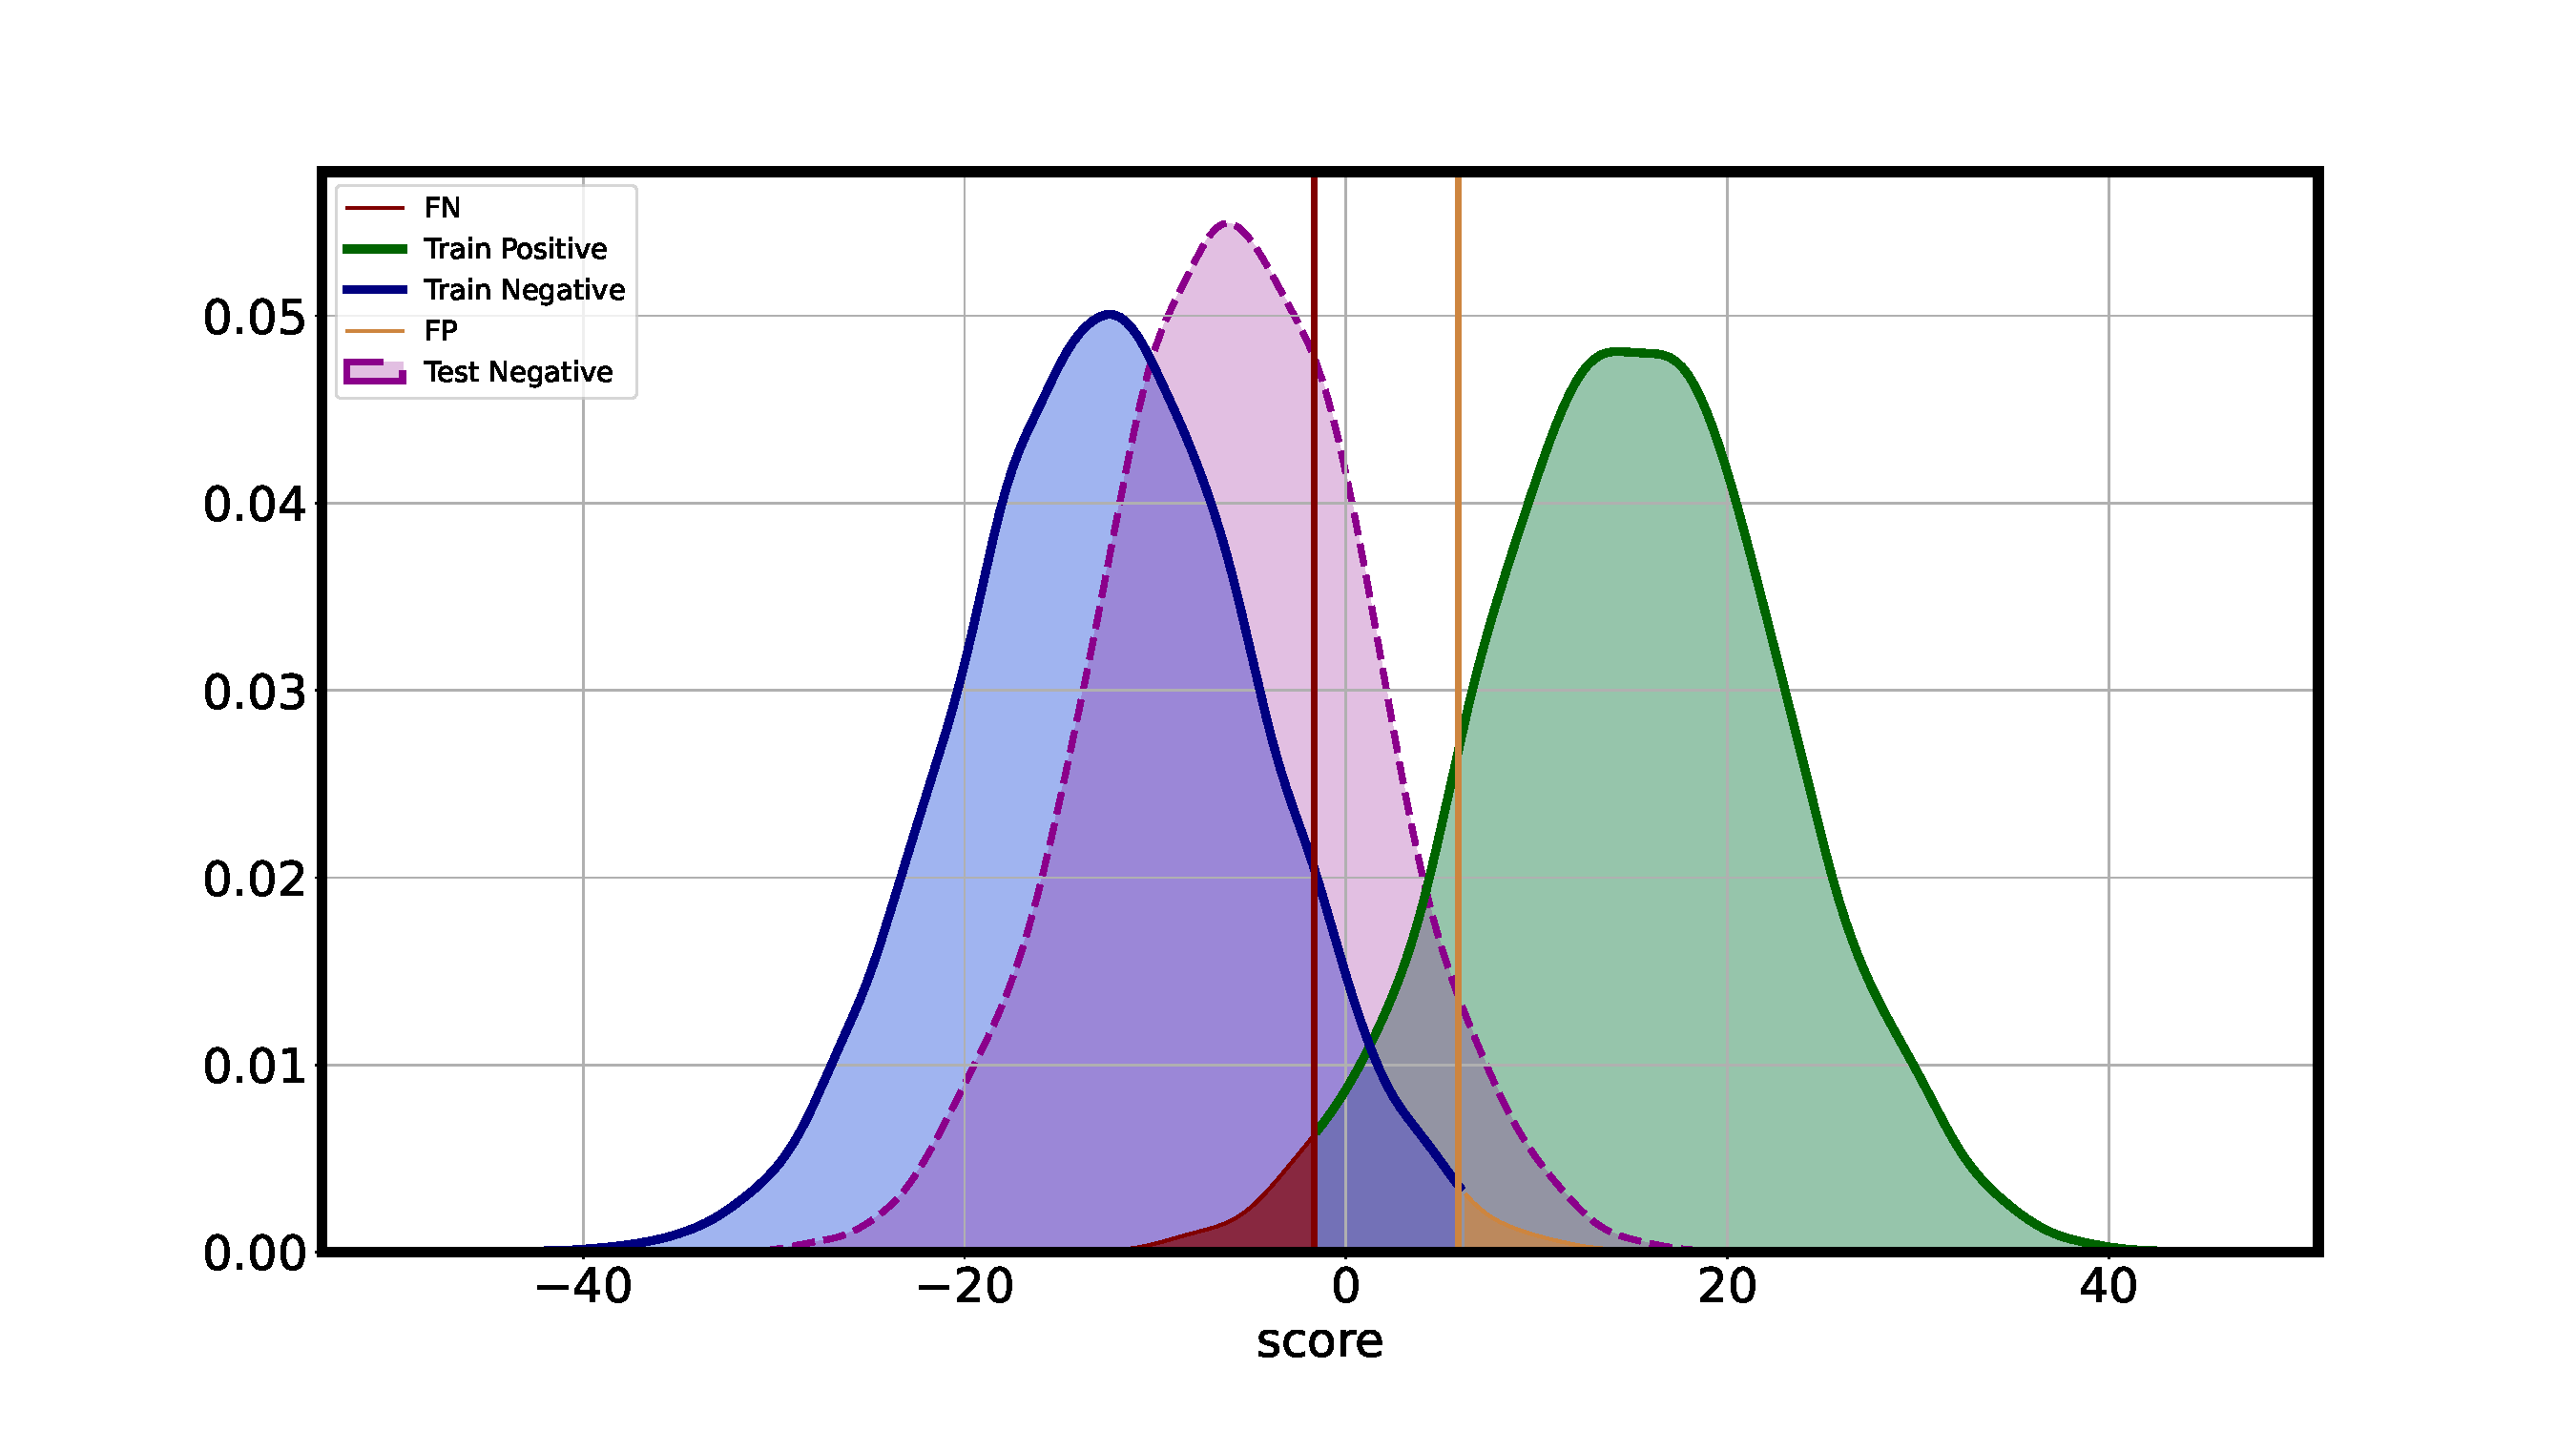
\includegraphics[width=5in]{img/synthetic_overview.pdf}
%	\caption{{\bf Error in decision making.} fd}
%	\label{fig:illustration}
%\end{figure}  


\section{Test null adjustment (TNA) method}
\subsection{Preliminaries}

Let us suppose that we are given domain $D$ such as images, text, speech, graphs, time series, tabular data, or the mix of these; furthermore, let $X\subseteq D$ and $T\subseteq D$ denote the training and  the test data samples, respectively. Let $Y_t\in\{0,1\}$ denote the true class label of sample $t\in D$. Let $f:D\rightarrow R$ be an appropriately trained binary discriminator (classifier), such as a deep neural network, to predict positive instances, where $R$ denotes the real numbers. Without loss of generality, we assume that higher score $f(t)$ indicates a stronger membership to the positive class. The training null distribution is constructed as $X_0=\{f(t):Y_t = 0,\,\,  t\in X\}$ from the scores of negative instances, the training target distribution is constructed as $X_1=\{f(t): Y_t = 1,\,\,  t\in X\}$ from the scores of positive instances, and the training score distribution is $X_s=\{f(t): t\in X\}$. The true test null $T_0$, true test target $T_1$, and the test score $T_s$ distributions are constructed in a similar way using true labels. We say that we trust (or accept) a  sample $t$ predicted as positive if and only if $f(t)>s_t$ for a given decision threshold  $s_t$ and we make indecision for samples if $f(t) < s_t$. The false discovery proportion (FDP) in a set of samples $K=\{t\in D\}$ at a score threshold $s_t$ is calculated as 
\begin{equation*}
	FDP(s_t,K)=\frac{1+|\{t\in K: Y_t=0,\,f(t)\ge s_t\}|}{|\{t\in K:f(t)\ge s_t\}|},
\end{equation*}
\noindent where $|.|$ denotes set cardinality. We reserve the FDR for the statistical expectation of FDP. FDR control methods aim to calibrate the threshold  $s_t$ so that the error rate among trusted predictions is at most level of $\alpha$. 

The empirical  p-values (EPVs) of the test samples are calculated using eq. \ref{eq:epv} with respect to $X_0$. The p-value calculation can be time consuming for large $X_0$ sets, in this case, a binned, empirical cumulative distribution function of $X_0$ could be used to calculate the p-values accordingly in an accelerated way. Then, the FDR of a set $T$ can be controlled using the $BH$ protocol and the EPVs at a predetermined $\alpha$ level. For the sake of simplicity, we replace the $\alpha$ with $\alpha/\hat{\pi_0}$ inside BH algorithm, where $\hat{\pi_0}$ is an estimation of $\pi_0$ introduced by Storey \cite{storey2004strong} in the following way: $\hat{\pi_0} = (1+\sum_{i=1}^m \mathone\{p_i\ge\lambda\} )/(m(1-\lambda))$ for $\lambda\in (0,1)$. The q-value of a test sample $t\in T$ is defined as $q_t=\min_{z\le f(t)}FDP( z, T )$; that is the minimum $\alpha$ level when the sample $t$ would become a trusted positive prediction. 
The smaller the q-value of a test sample $t$ is, the more trusted positive prediction $t$ is. Note that, the q-value of a sample depends not only on its prediction score, but also on the other samples in the set. 
%
% THIS IS WITH MULTI CLASS CLASSIFICATION
%Let us suppose that we are given a domain $D$ such as images, text, speech, graphs, time series, tabular data, or the mix of these; furthermore, let $X\subseteq D$ and $T\subseteq D$ denote the training and  the test data samples, respectively. Let $Y_t\in\{0,\dots, K-1\}$ denote the true class label of sample $t\in D$. Let $f_k:D\rightarrow R$ be appropriately trained discriminators (classifiers), such as a deep neural network, to indicate class memberships ($k=0,1,\dots,K-1$), where $R$ denotes the real values. Without loss of generality, we assume that higher score $f_k(t)$ indicates a stronger membership to class $k$. Then, let $f(t)= \max_k\{f_k(t) \}$ and $L(t)=\text{argmax}_k\{f_k(t)\}$ be the predicted class label for $t\in D$. The train null distribution is constructed as $N_0=\{f(t): L(t) \ne Y_t,\,\,  t\in X\}$ from the scores of incorrect classifications, the train target distribution is constructed as $N_1=\{f(t): L(t) = Y_t,\,\,  t\in X\}$ from the scores of correct classifications. The true test null and true test target distributions are constructed in a similar way from the test samples with using the true labels, respectively.  We say that, we trust a prediction $L(t)$ for a sample $t$  if $f(t)\ge s_t$ for a decision threshold $s_t$, and we make indecision for samples if $f(t) < s_t$. The false discovery proportion (FDP) in a set of samples $\{t\in D\}$ at a score threshold $s_t$ is calculated as 
%\begin{equation}
%	FDP(s_t)=\frac{1+|\{t: Y_t\ne L(t),\,f(t)\ge s_t\}|}{|\{t:f(t)\ge s_t\}|},
%\end{equation}
%\noindent where $|.|$ denotes set cardinality. We reserve the FDR for the statistical expectation of FDP. FDR control aims to calibrate the $s_t$ so that the error rate among trusted predictions is at level of $\alpha$. We note that FDR control is related to FSR control in this case, even for $K=2$.%False positives are calculated as $FP=|\{t:Y_t\ne L(t)\}|$
%%A label of a sample $t\in D$ is predicted $L(t)=sign(f(t))$. Let $N_0=\{f(t):t\in X,\, Y_t=0\}$,  the null distribution; that is, the set of the discriminative scores of the negative training samples.
%
%For binary classification problems (K=2), let $f:D\rightarrow R$ be a trained discriminator (classifier), $N_0=\{f(t):t\in X,\, Y_t=0\}$ the train null distribution,  $N_1=\{f(t):t\in X,\, Y_t=1\}$ the train target distribution, and $FDP(s_t)=(1+{|\{t: Y_t=0,\,f(t)\ge s_t\}|)/|\{t:f(t)\ge s_t\}|}$. We say that we trust the positive prediction of sample $t$ if and only if $f(t)>s_t$. We note that the FDR control is not related to FSR control in this case. 
%
%The p-values of the test samples are calculated with using eq. \ref{eq:epv} with respect to $N_0$. The p-value calculation can be time consuming for large $N_0$ sets, in this case, a binned, empirical cumulative distribution function of $N_0$ could be used to calculate the p-values accordingly. The FDR in a set $T$ can be controlled with using the $BH$ protocol at a predetermined $\alpha$ level. For the sake of simplicity, we replace the $\alpha$ with $\alpha/\hat{\pi_0}$ inside BH algorithm, where $\hat{\pi_0}$ is an estimation of $\pi_0$ introduced by Storey \cite{storey2004strong}: $\hat{\pi_0} = (1+\sum_{i=1}^m \mathone\{p_i\ge\lambda\} )/(m(1-\lambda))$ for $\lambda\in (0,1)$. The q-value of a test sample $t\in T$ is defined as $q_t=\min_{z:\le f(t)}FDP( z )$, that is the minimum $\alpha$ level when the sample $t$ would become a trusted prediction. The q-value of a sample would depend on the other samples in the set. The lower the q-value the most trusted the prediction is.

%\paragraph{Example 1.} For demonstration, we trained a two-layer convolutional neural network containing 8 kernels with size of $3\times3$ at each layers, respectively, to predict the hand-written digits of the MNIST samples. The MNIST dataset contains 60K training and 10K test images of 28x28 pixels in 10 classes. There is no shift in the test set. The accuracy of the trained model is 0.975. The score distributions 

\paragraph{Learn-then-test (LTT).} We acquired the LTT code from its authors' GitHub repository. We  specified the following hyperparameters as following: 100 uniformly distributed queried levels of FDR control are iteratively being processed, starting from the 1e-3, with the most appropriate threshold $\lambda$ being selected among the 300 potential threshold values for each iteration. The remainder of the methodology is entirely dependent on the published pipeline, including the comprehensive calculation of the p-values for each threshold during each alpha level test, with a further Bonferroni procedure employed to select the most appropriate border. The final value of the test false positive rate is equal to the number of samples with higher scores than the selected $\lambda$. 

\paragraph{Example 	 1.} \label{ex:vanilla} We used the well-known MNIST dataset for demonstration. It contains 60K training and 10K test images of 28x28 grey-scaled pixels in 10 classes. There is no data or label shift between the training and test data. We trained a convolutional neural network to classify the digit '1' as target (positive) against all the other digits (negative) (binary classification for the sake of simplicity). Our ConvNet model contained two convolutional layers consisting of 8 kernels with size of $3\times3$ each, and it was trained with an Adam optimizer with a learning rate of 0.01 for three epochs. Our trained model achieved a 99\% accuracy on the test set. 

The relevant results are presented in Figure \ref{fig:binary}. Figure \ref{fig:binary}A shows the training and test null and target distributions. %This plot indicates that there is no shift between the training and test distributions. 
Figure \ref{fig:binary}B shows a Q-Q plot of the test EPVs against the theoretical uniform distribution; that is the scatter plot of the EPV against its normalized rank in our case. The dots line up along the diagonal line which shows that the EPVs calculated are uniformly distributed and, consequently, valid. This also indicates that there is no shift between the training and test distributions. %We also performed the Fisher's combined test to check whether the empirical p-values are uniformly distribution. The test produces a p-value of 0.934 indicating uniformly distributed empirical p-values. 
Figure \ref{fig:binary}C shows the number of accepted (trusted) predictions as positives at various q-values ($\alpha$ level of FDR). The ground truth (black solid line) was calculated using the true test labels. Any FDR controlling method (a) yielding more trusted predictions than the ground truth is implied to be liberally biased, and (b) yielding less trusted predictions is conservatively biased. The BH procedure with EPVs (red dashed line) yields closely the same number of trusted predictions at various FDR levels of $\alpha$ (calculated without using the true test labels). This repeatedly indicates that the EPVs are uniform and the  BH procedure is an unbiased method. The LTT method also accurately controls the FDR at any $\alpha$ levels (blue dotted line). Finally, Figure \ref{fig:binary}D shows that the deviation of the estimated FDPs from the true FDPs is small.



\begin{figure}
	\centering
	\begin{tabular}{cccc}
		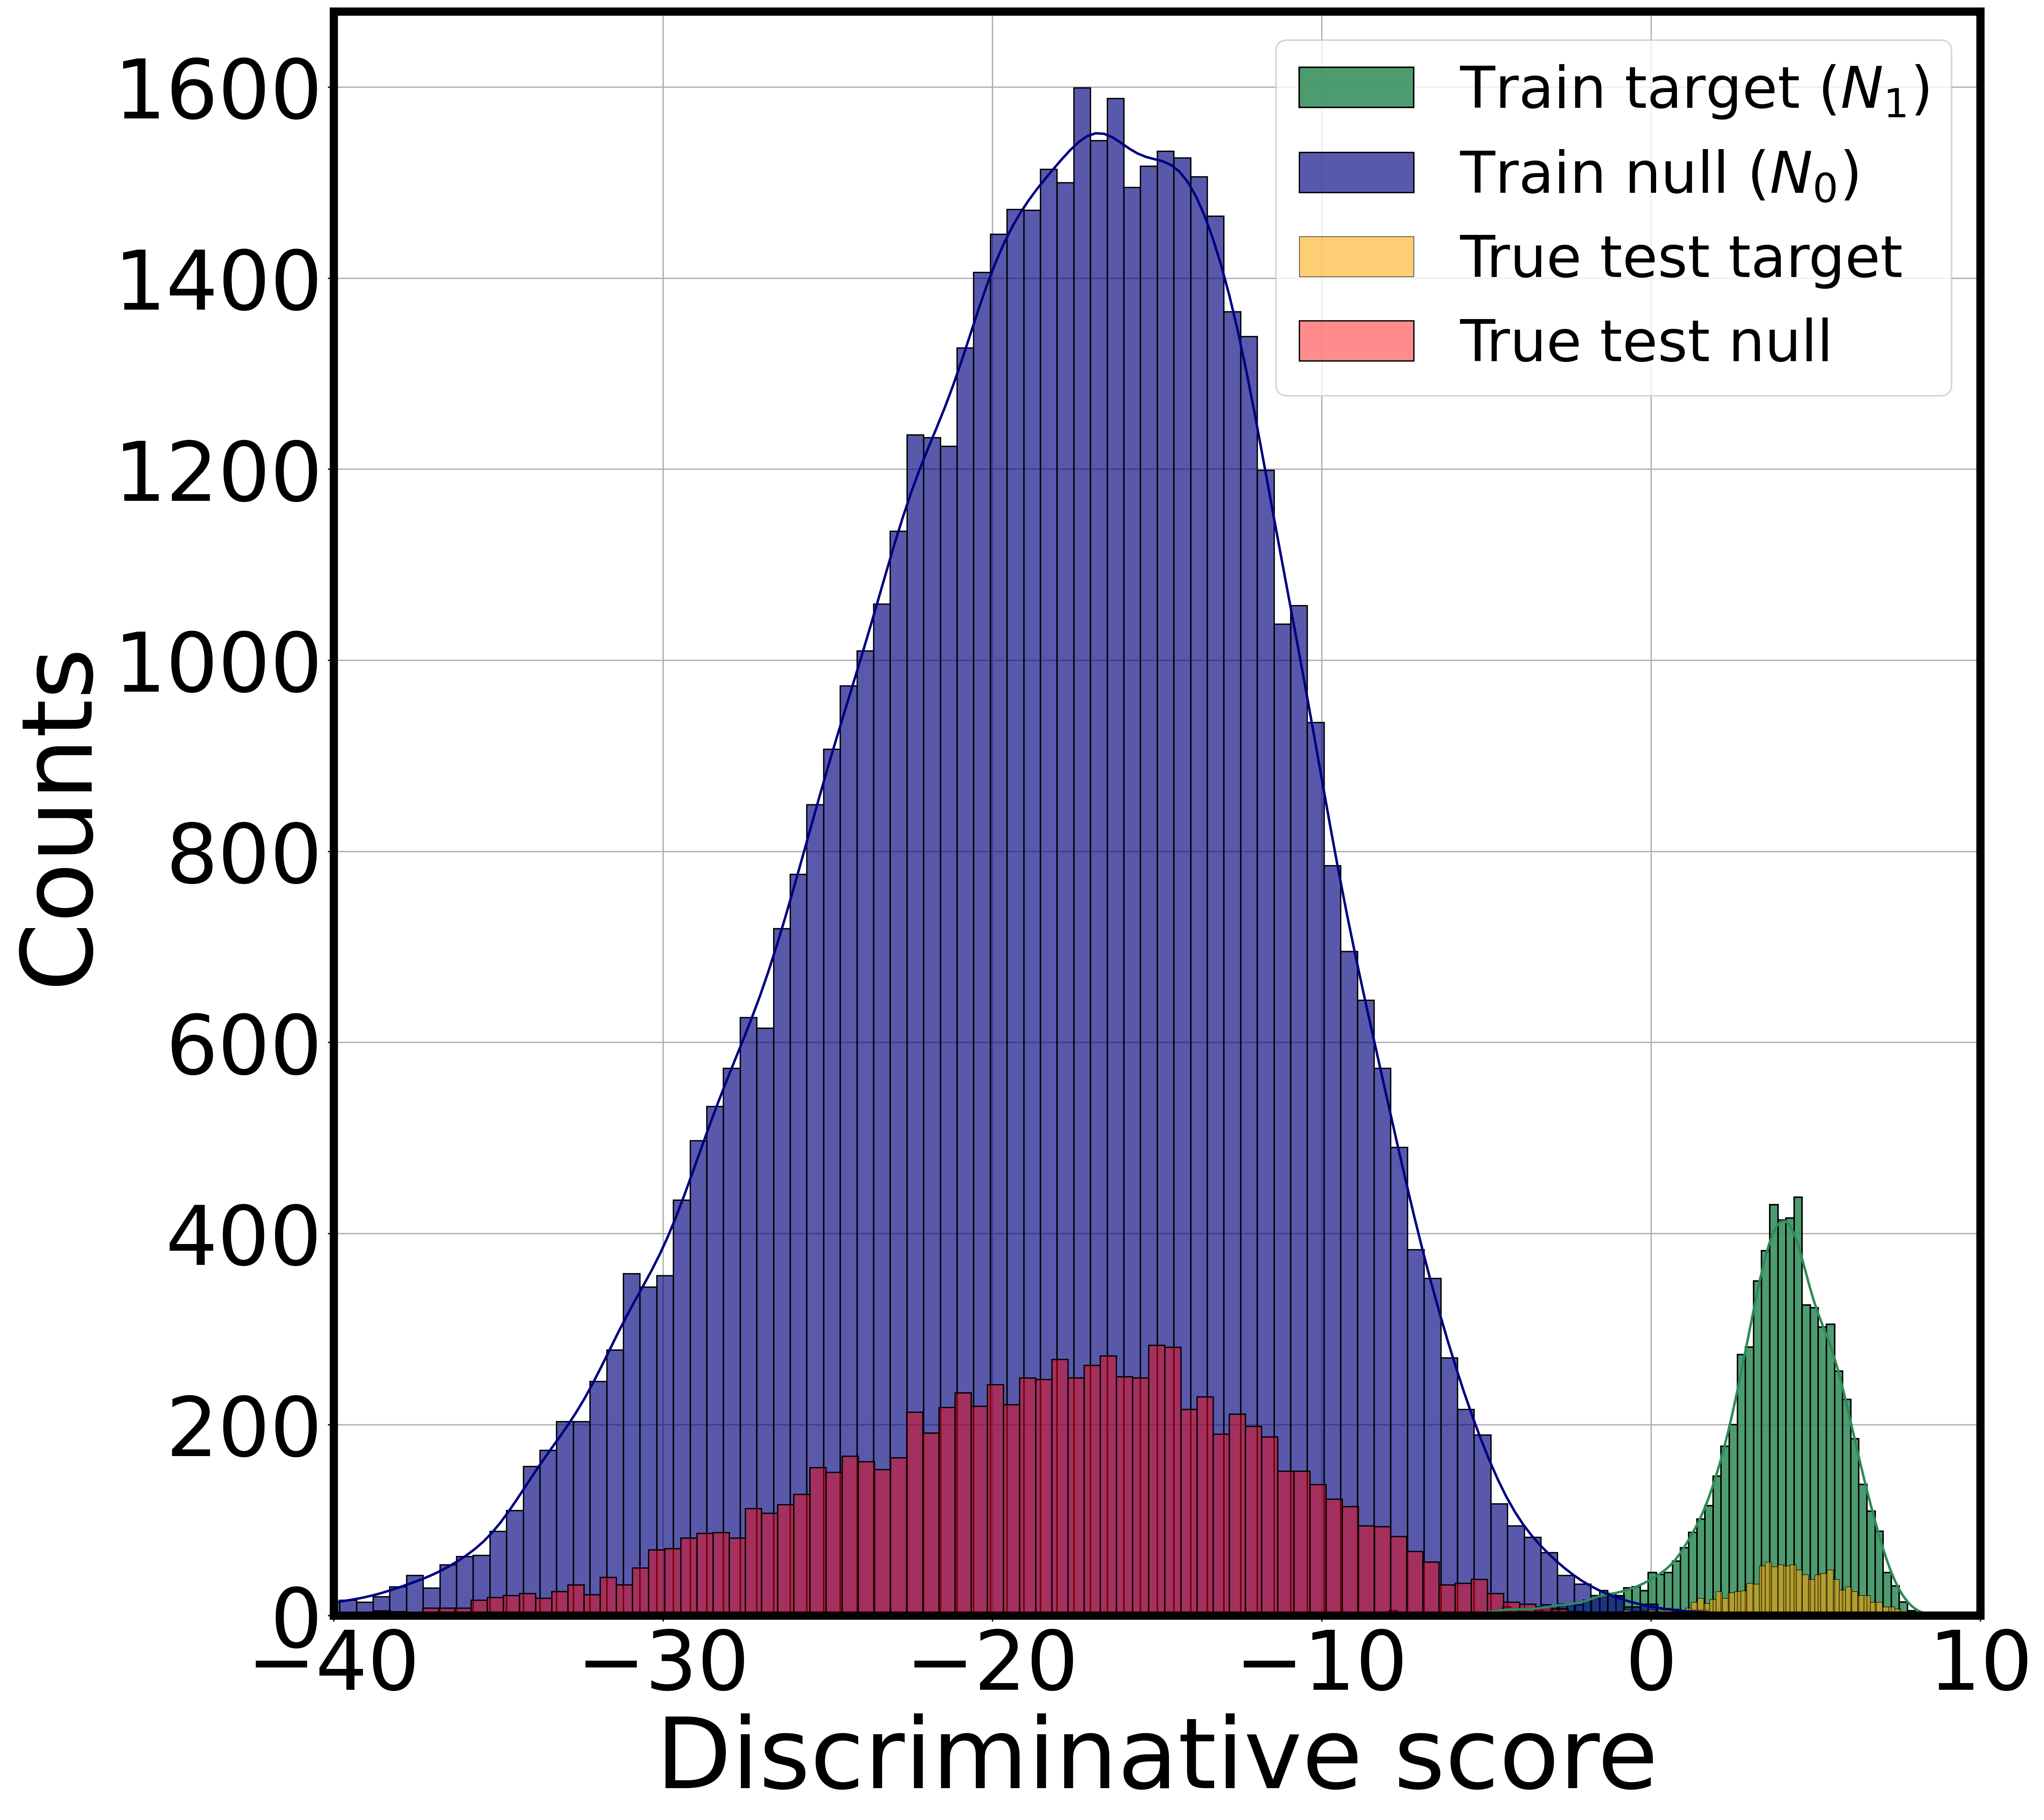
\includegraphics[width=1.78in]{img/cls_overview.png}&
		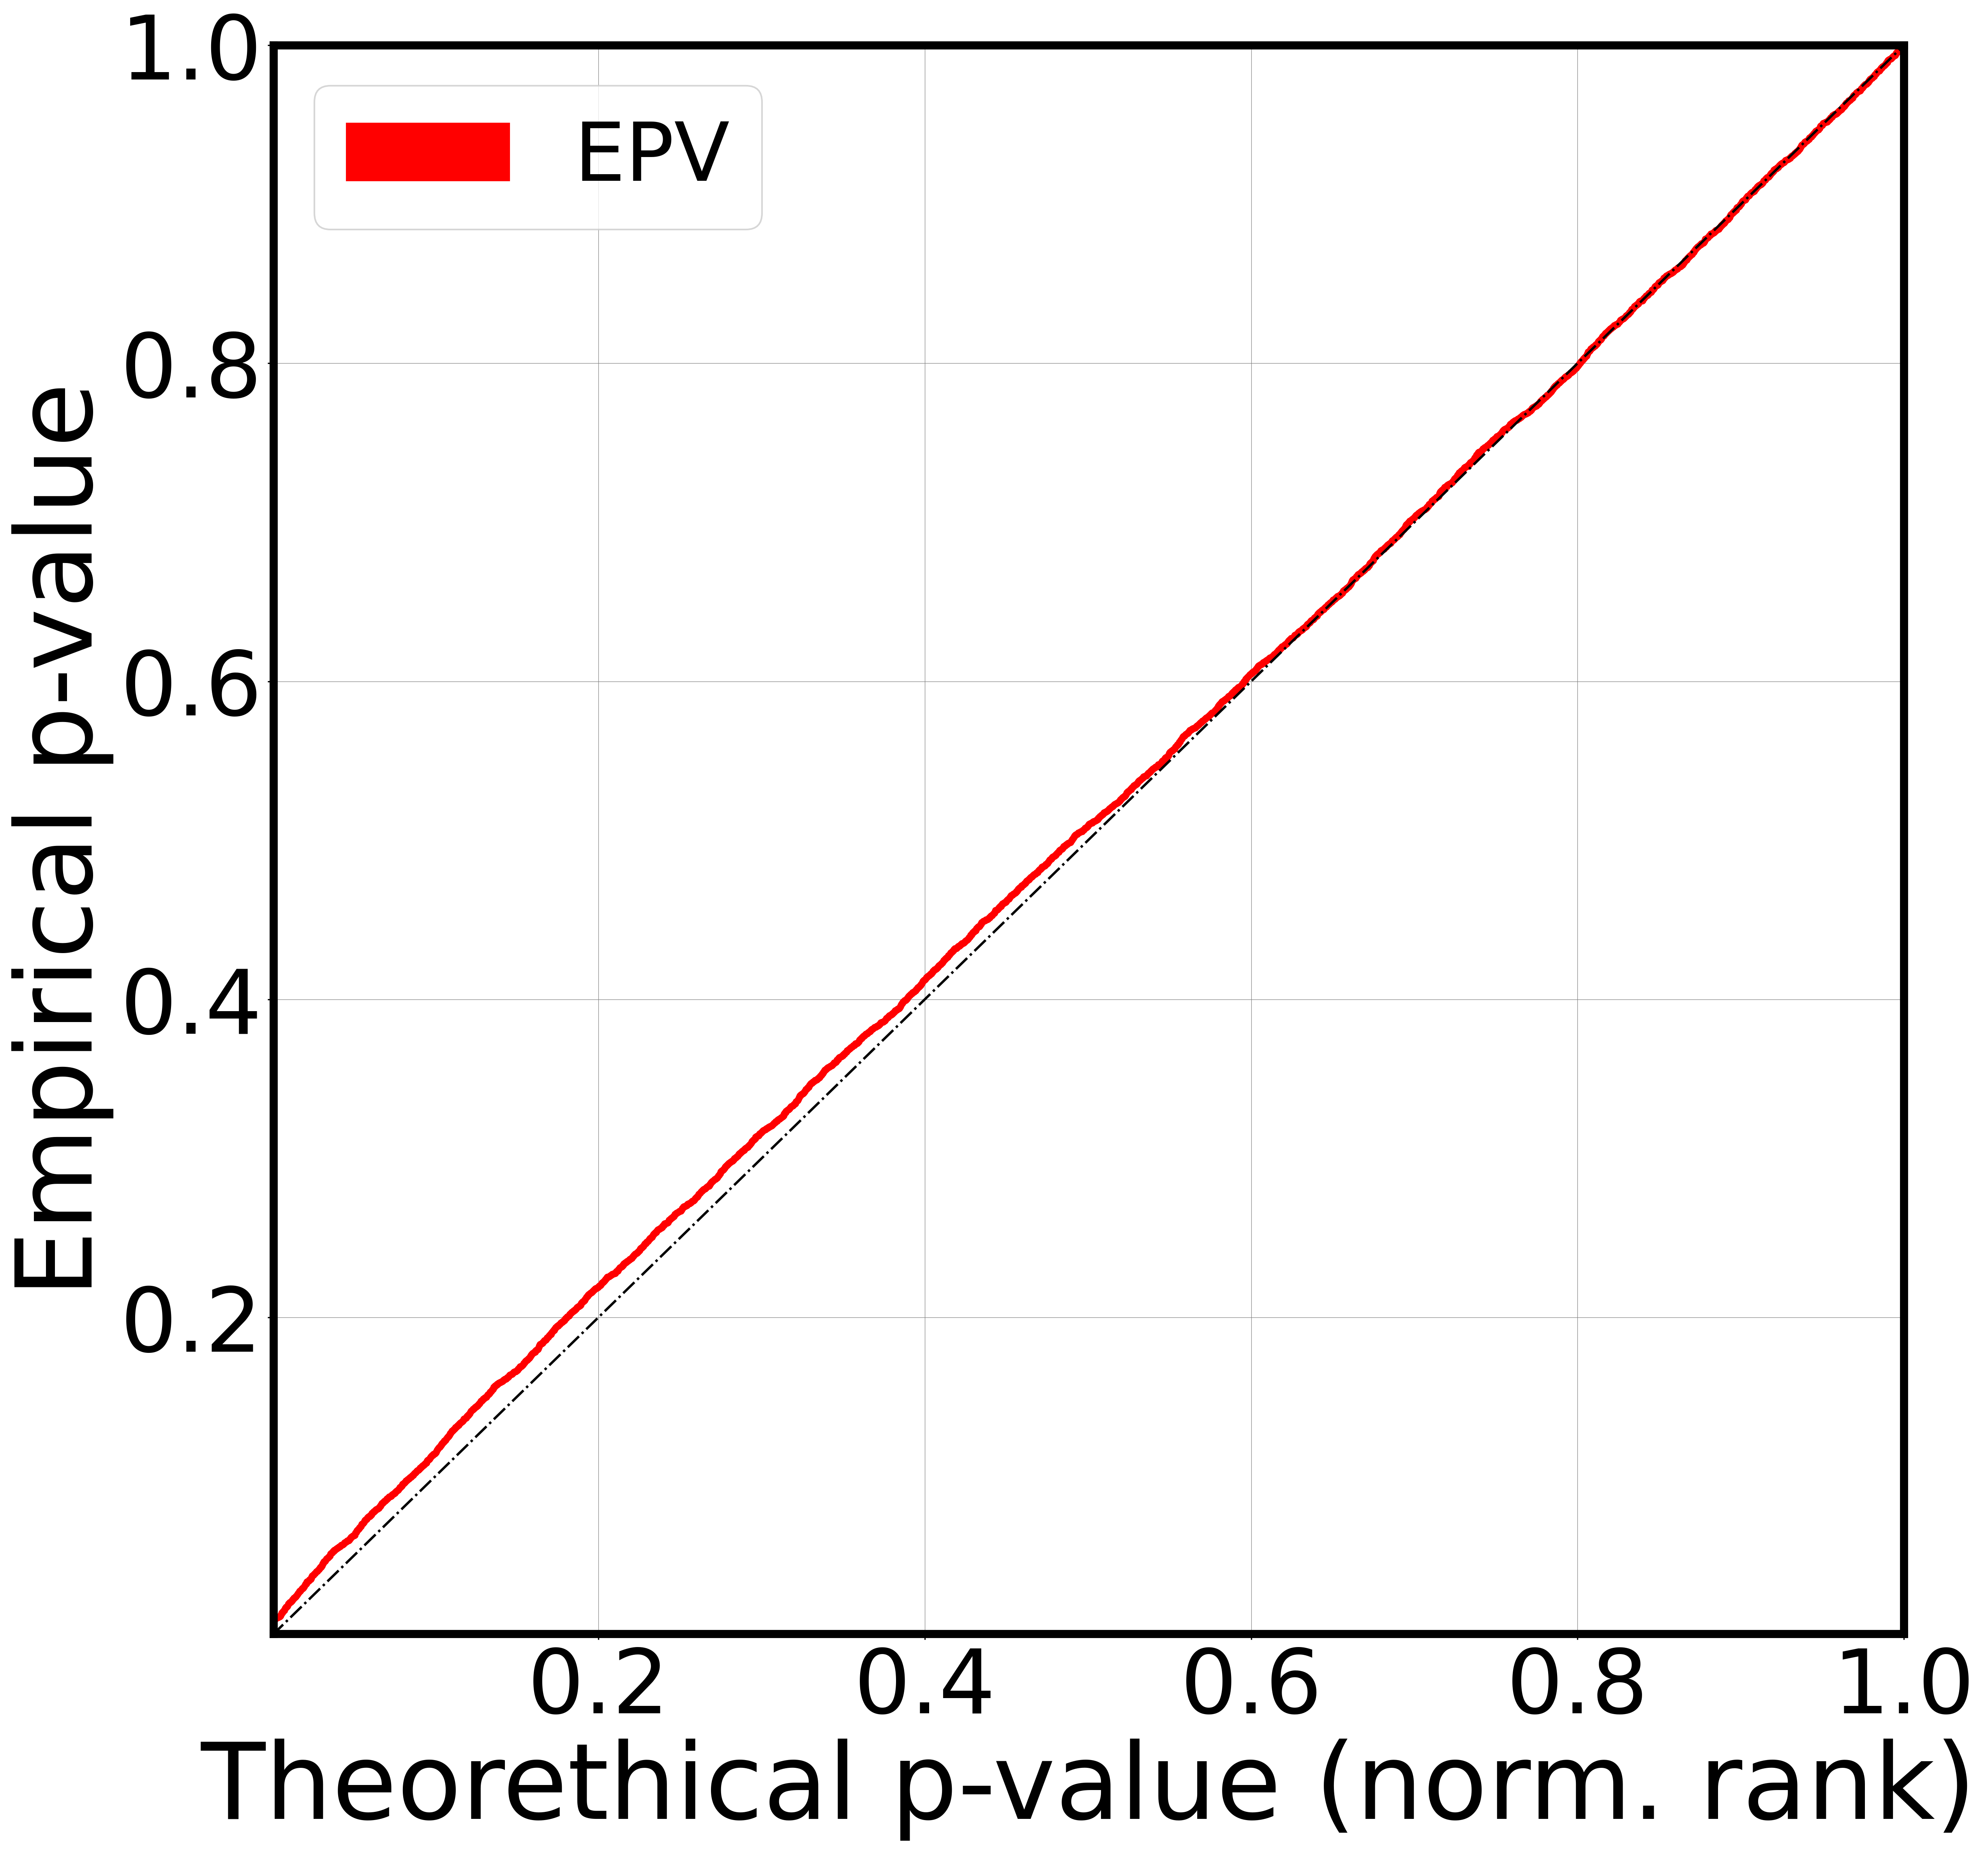
\includegraphics[width=1.73in]{img/cnn_QQ_classical.png} &
		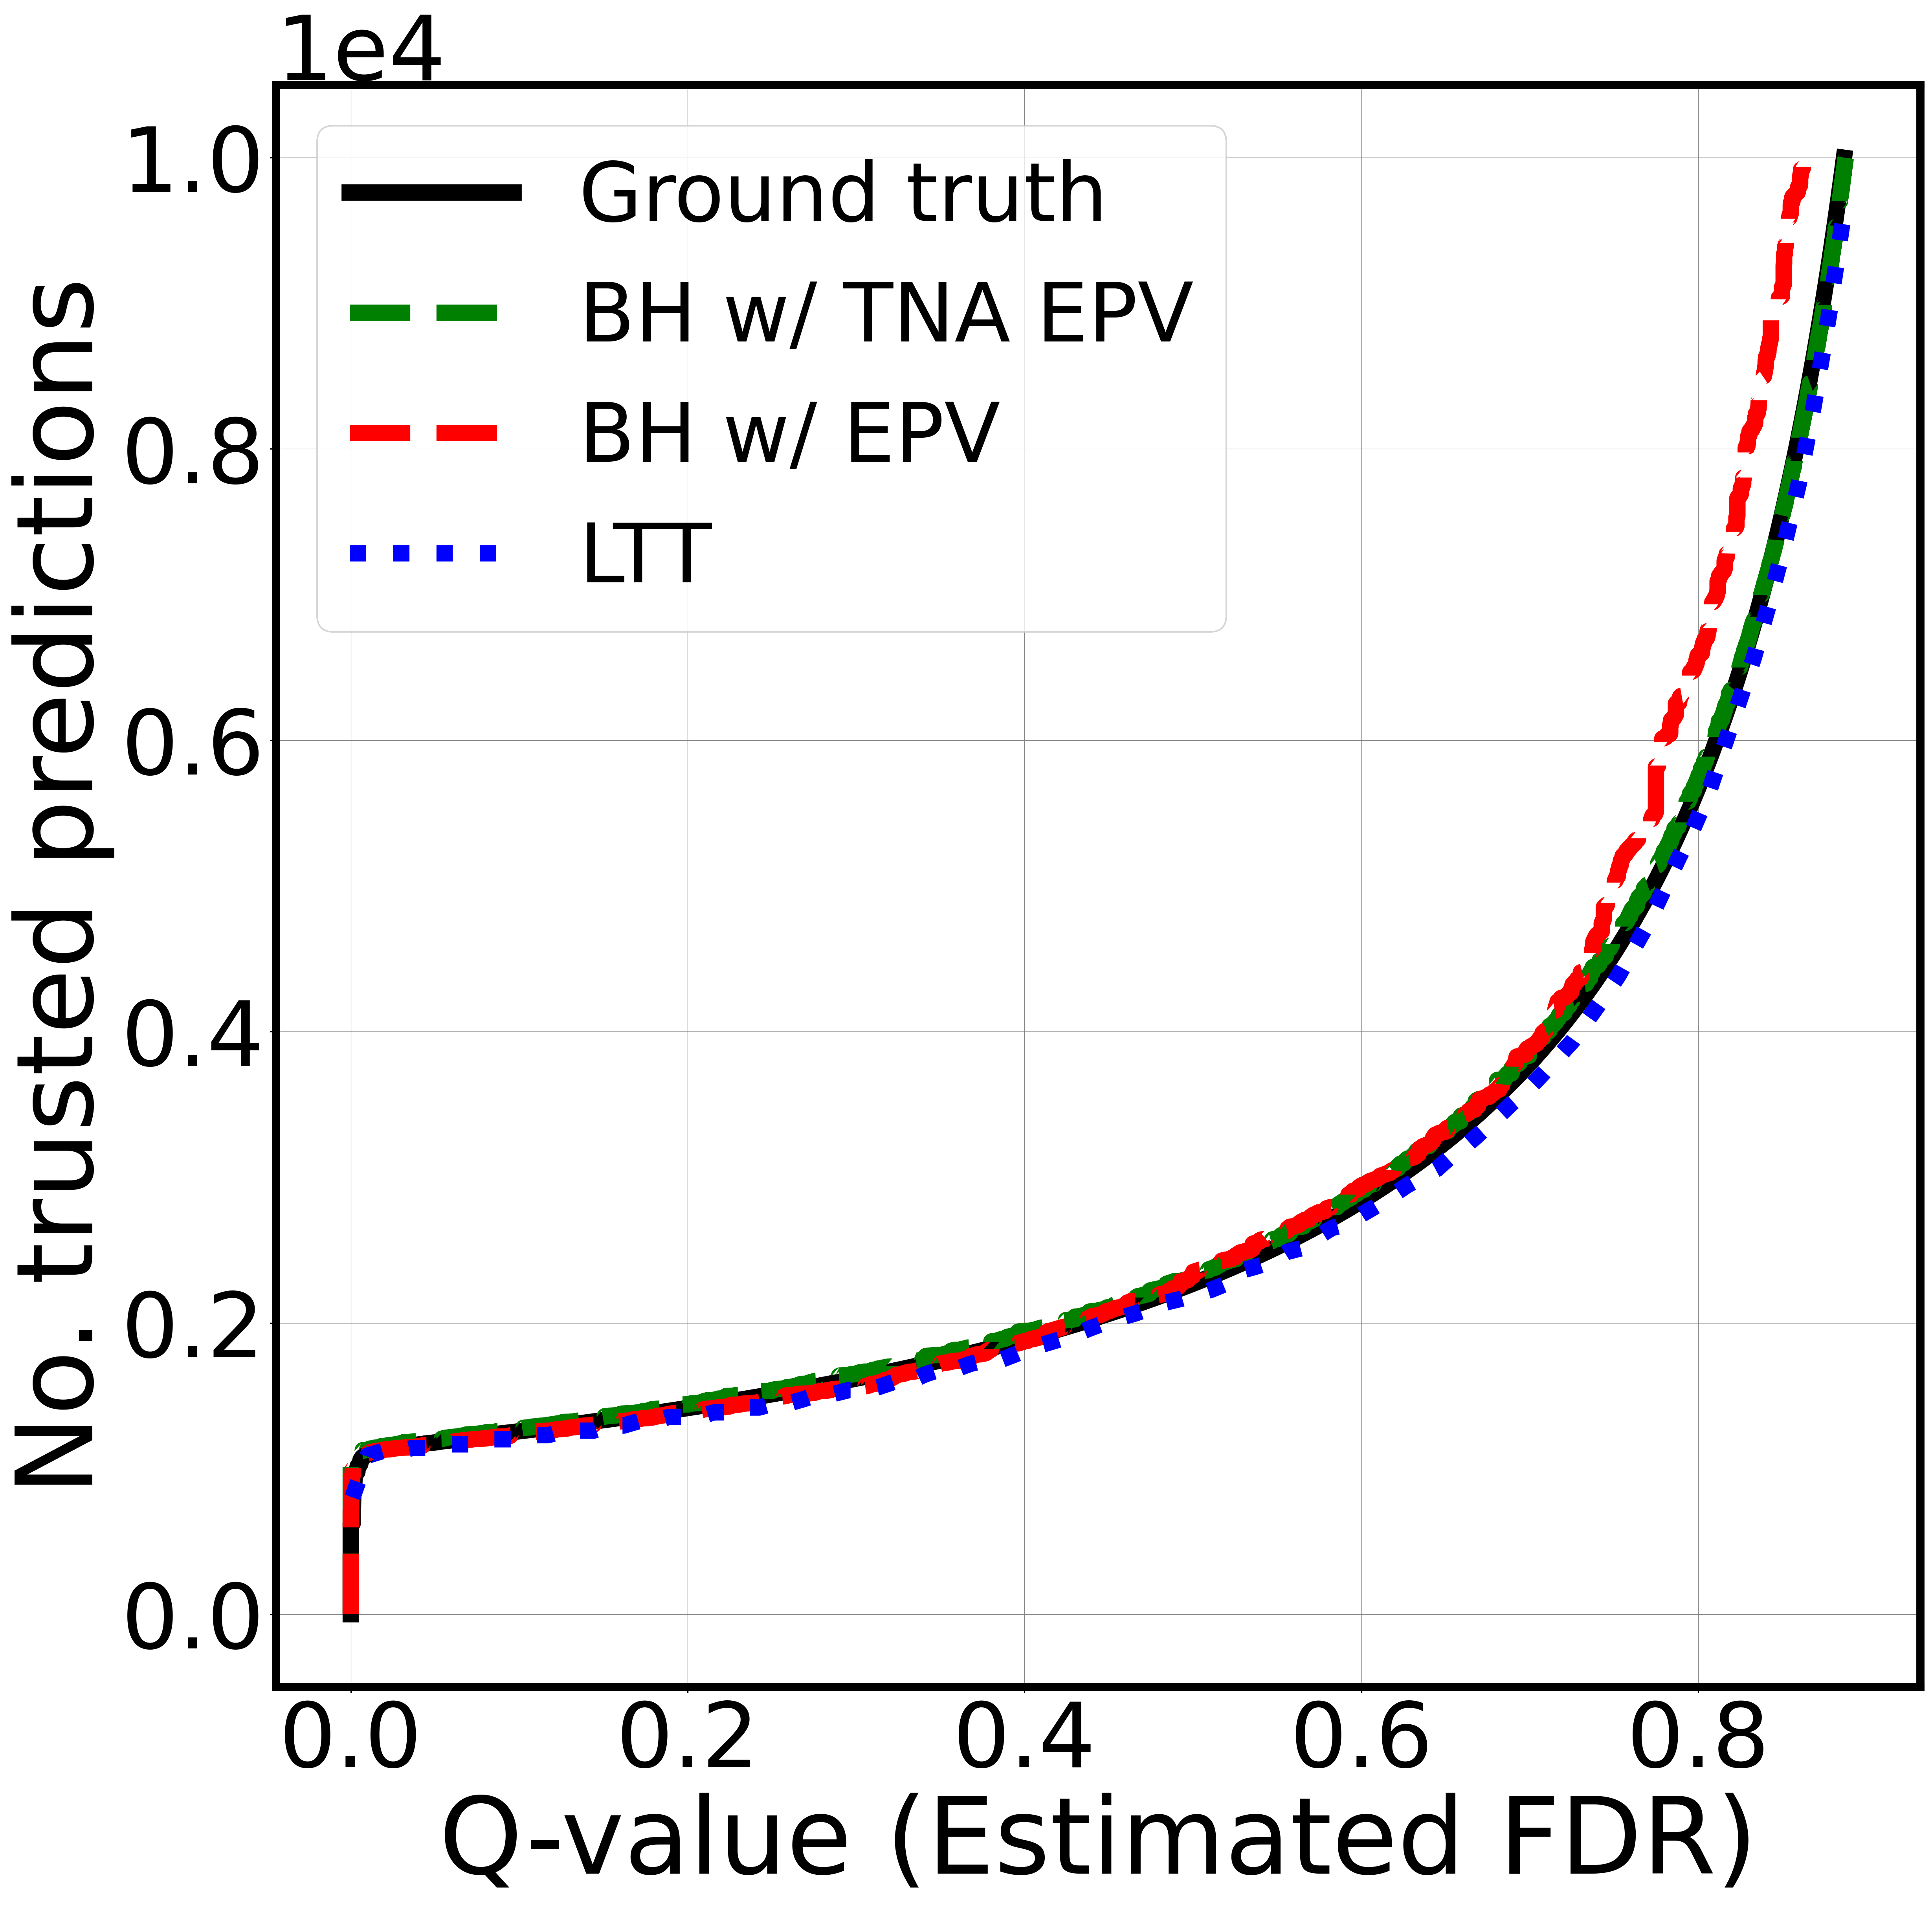
\includegraphics[width=1.69in]{img/cnn_classical_fdr_control.png} &
		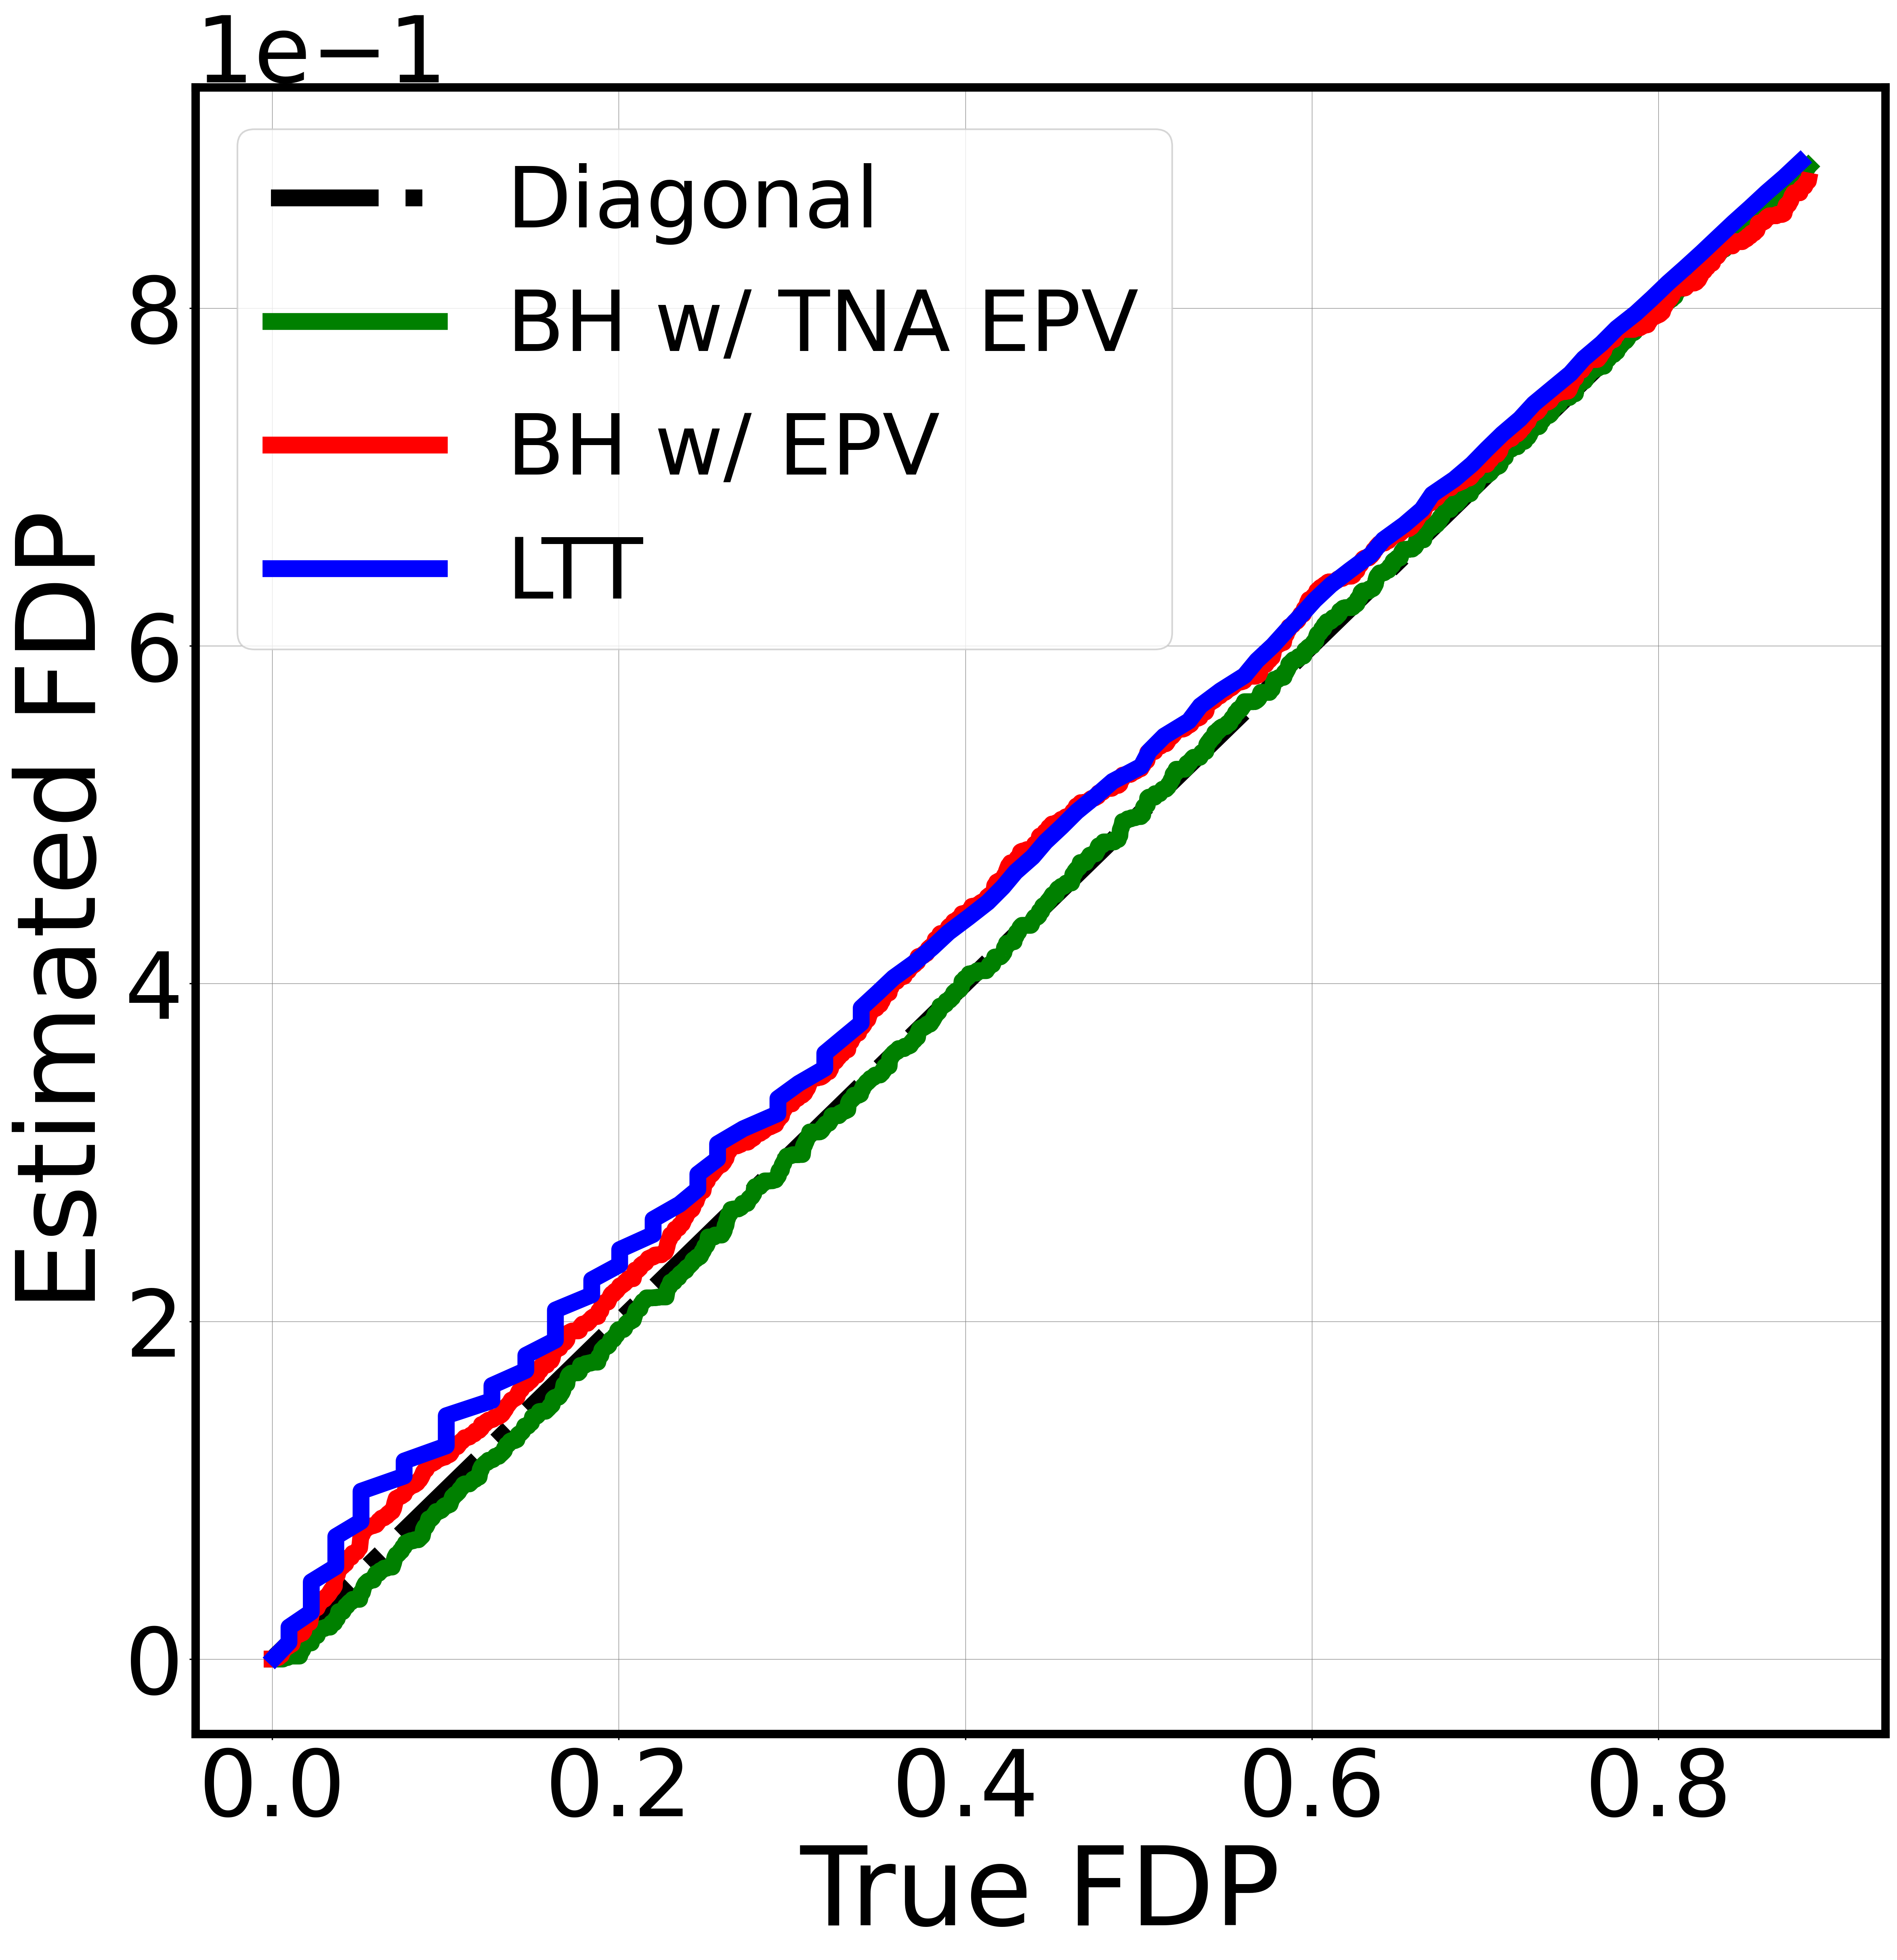
\includegraphics[width=1.68in]{img/cnn_FDPscat_classical.png} \\
		A & B & C & D \\
	\end{tabular}
	\caption{{\bf FDR control in MNIST with EPVs. } (A) The discriminative score distributions. (B) The Q-Q plot of the EPVs of the test samples against the theoretical uniform distribution. (C) The number of the accepted (trusted) positive predictions at various q-values calculated with true labels (black solid line), BH with EPVs (red dashed line), and LTT (blue dotted line). (D) Deviation between the true and the estimated FDR produced by BH with EPV (red line) and LTT (blue dots), respectively.}
	\label{fig:binary}
\end{figure}
 
\paragraph{TNA protocol.} When the training null distribution $X_0$ is different from the test null distribution $T_0$, the EPVs will not be uniformly distributed and the BH procedure results in liberal or conservative bias in FDR estimation. In the following steps, we describe two versions of TNA methods that both adjusts the prediction scores so that the approximated test null distribution $\hat{T}_0$ aligns to the actual training null distribution $X_0$. The first variation, called TNA- (TNA minus), relies on the train null ($X_0$) distribution, while the TNA+ (TNA plus) relies on the train target ($X_1$)distribution. The two approaches differ only at the 3rd step of the following algorithm. 

\begin{enumerate}%[label=\arabic*.]
	\itemsep-3pt  		
	\item [1.] Get the density histograms of $X_0$, $X_1$, and $T_s$ distributions with identical bin borders and denote them as $\overline{X}_0$, $\overline{X}_1$, and $\overline{T}_s$, respectively. The $\overline{X}[i]$ denotes the value of bin $i$.  We used 100 bins in our experiments.
	
	\item [2.] Let $\hat{\pi}_0$ be an approximated proportions of the negative test predictions calculated using the number of positive and negative test predictions. 
	
	\item [3a.] TNA-:  We create a new density histogram $\hat{T}_0$ that will be an approximation of the test null $T_0$. The value of the histogram bin $i$ is calculated  by $\hat{T}_0[i] = \overline{T}_s[i]\cdot c[i]$, where $c[i]=X_0[i]/X_s[i]$ is the proportion of the null samples in the mixture distribution.
	\item [3b.] TNA+: This approach relies on the following formulation: $X_s = (\pi_0) \cdot X_0 + (1-\pi_0) \cdot X_1$, where $\pi_0$ is the proportion of the negative samples; therefore, the null distribution can be expressed as $X_0 = (X_s - (1-\pi_0) \cdot X_1)/\pi_0$. We create a new density histogram $\hat{T}_0$ that will be an approximation of the test null $T_0$. The value of the histogram bin $i$ is calculated  by $\hat{T}_0[i] = (\overline{T}_s[i] -  (1-\hat{\pi}_0)\hat{T_1}[i])/\hat{\pi}_0$. The unknown $\hat{T_1}$ is approximated by $T_s$ scaled with the proportion of the target calculated from the training data; that is:  $$\hat{T_1}[i] = \overline{T_s}[i]\cdot \frac {\overline{X_1}[i]}{\hat{\pi}_0 \overline{X_0}[i] + (1-\hat{\pi}_0) \overline{X_1}[i]}.$$ Mind that the training null and target distributions ($X_0, X_1$) are weighted with test class proportions  $\hat{\pi}_0$. The outcome of division by zero is set to zero.
		
	\item [4.] Let $\mu_{X_0}$, $\sigma_{X_0}$, $\mu_{\hat{T_0}}$, and $\sigma_{\hat{T_0}}$ are the mean and std of the $X_0$ and the $\hat{T_0}$ distributions, respectively. 
	
	\item [5.] Adjust the test scores $\hat{t_s} = (t_s-\mu_{\hat{T_0}})/\sigma_{\hat{T_0}} \cdot \sigma_{\hat{X_0}} + \mu_{X_0}$.
\end{enumerate}

	Finally, calculate the TNA EPVs for each $\hat{t_s}$ with respect to the $X_0$ distribution, estimate  $\hat{\pi_0}$ for the test instances with the Storey method with $\lambda= 0.8$, and run BH procedure to control the FDR at a desired level. 
	
	We also note that we tested a one-dimensional optimal transportation (OT) to adjust train null to test null. Unfortunately, this approach is very sensitive to the test null approximation especially at the decision boundary. In our experiment, OT severely overfitted, while TNA remained more robust to poor tail approximation of the null distributions. OT did not provide any good results (data not shown) in our benchmark. 
	

\begin{figure}[h!]
	\centering
	\begin{tabular}{cccc}
		\multicolumn{4}{l}{\bf (i) Data distribution shift:}\\
		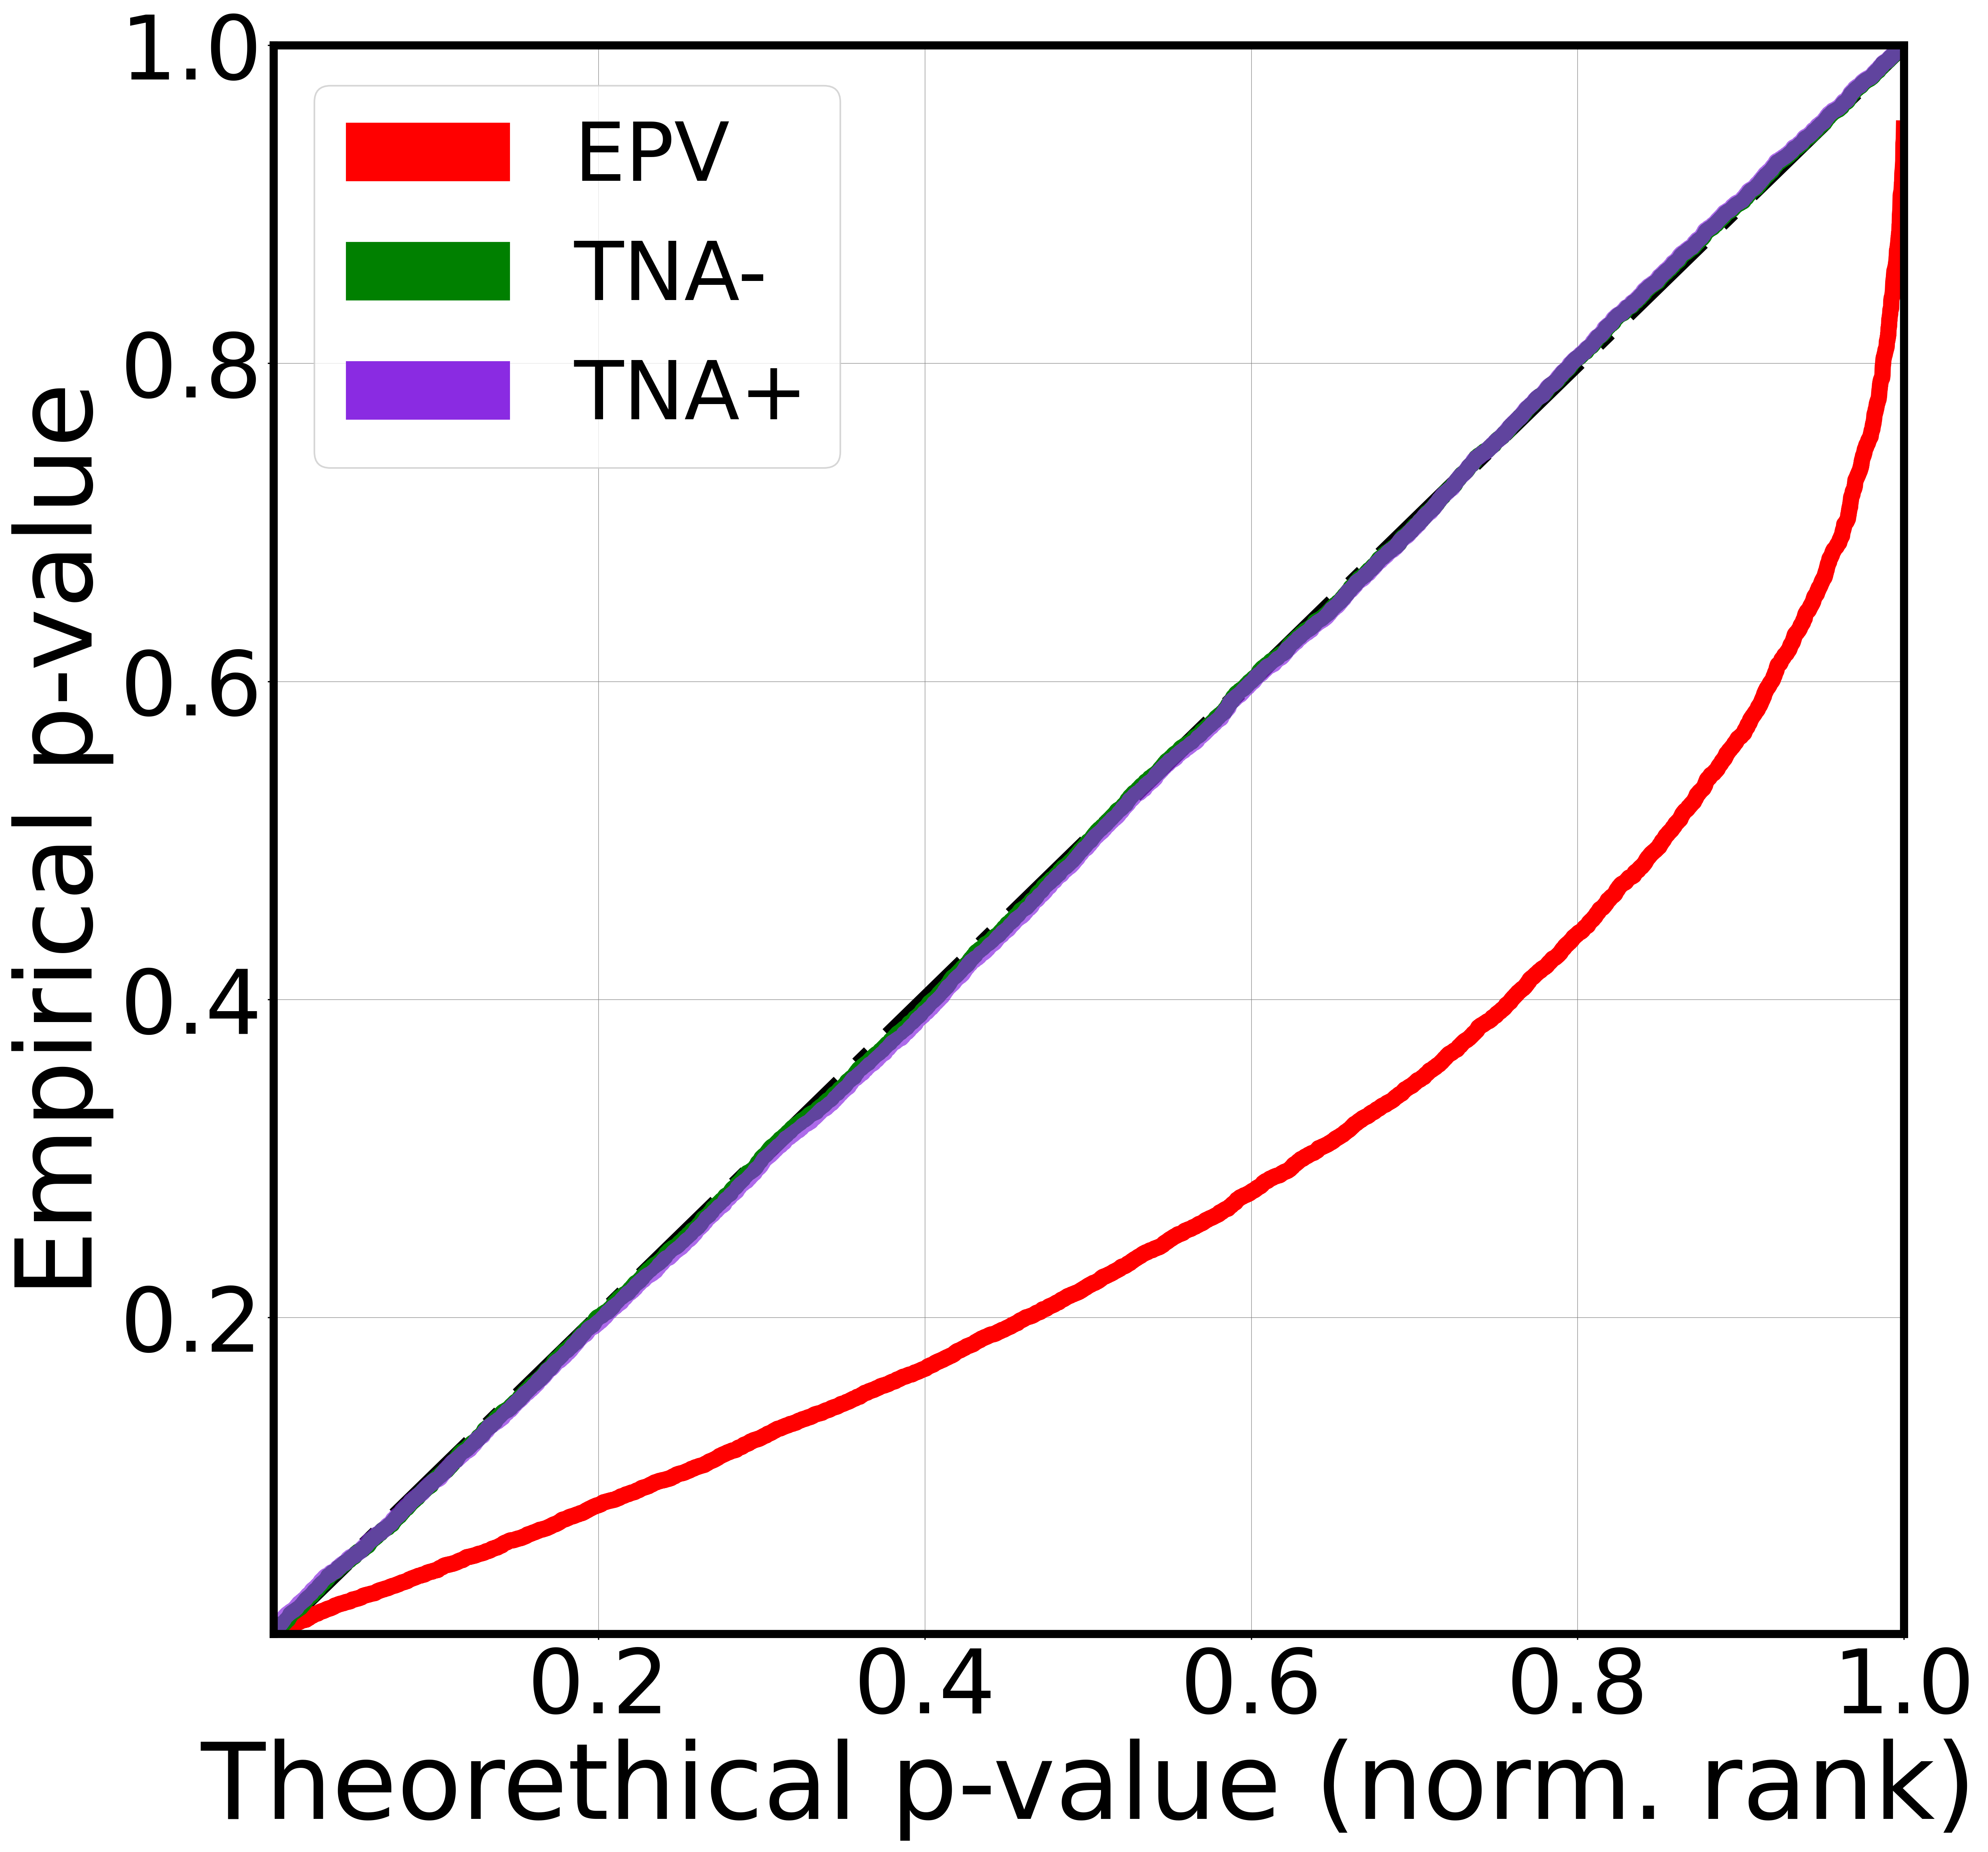
\includegraphics[width=0.225\linewidth, height=0.225\linewidth]{img/cnn_QQ_shifted.png}&
		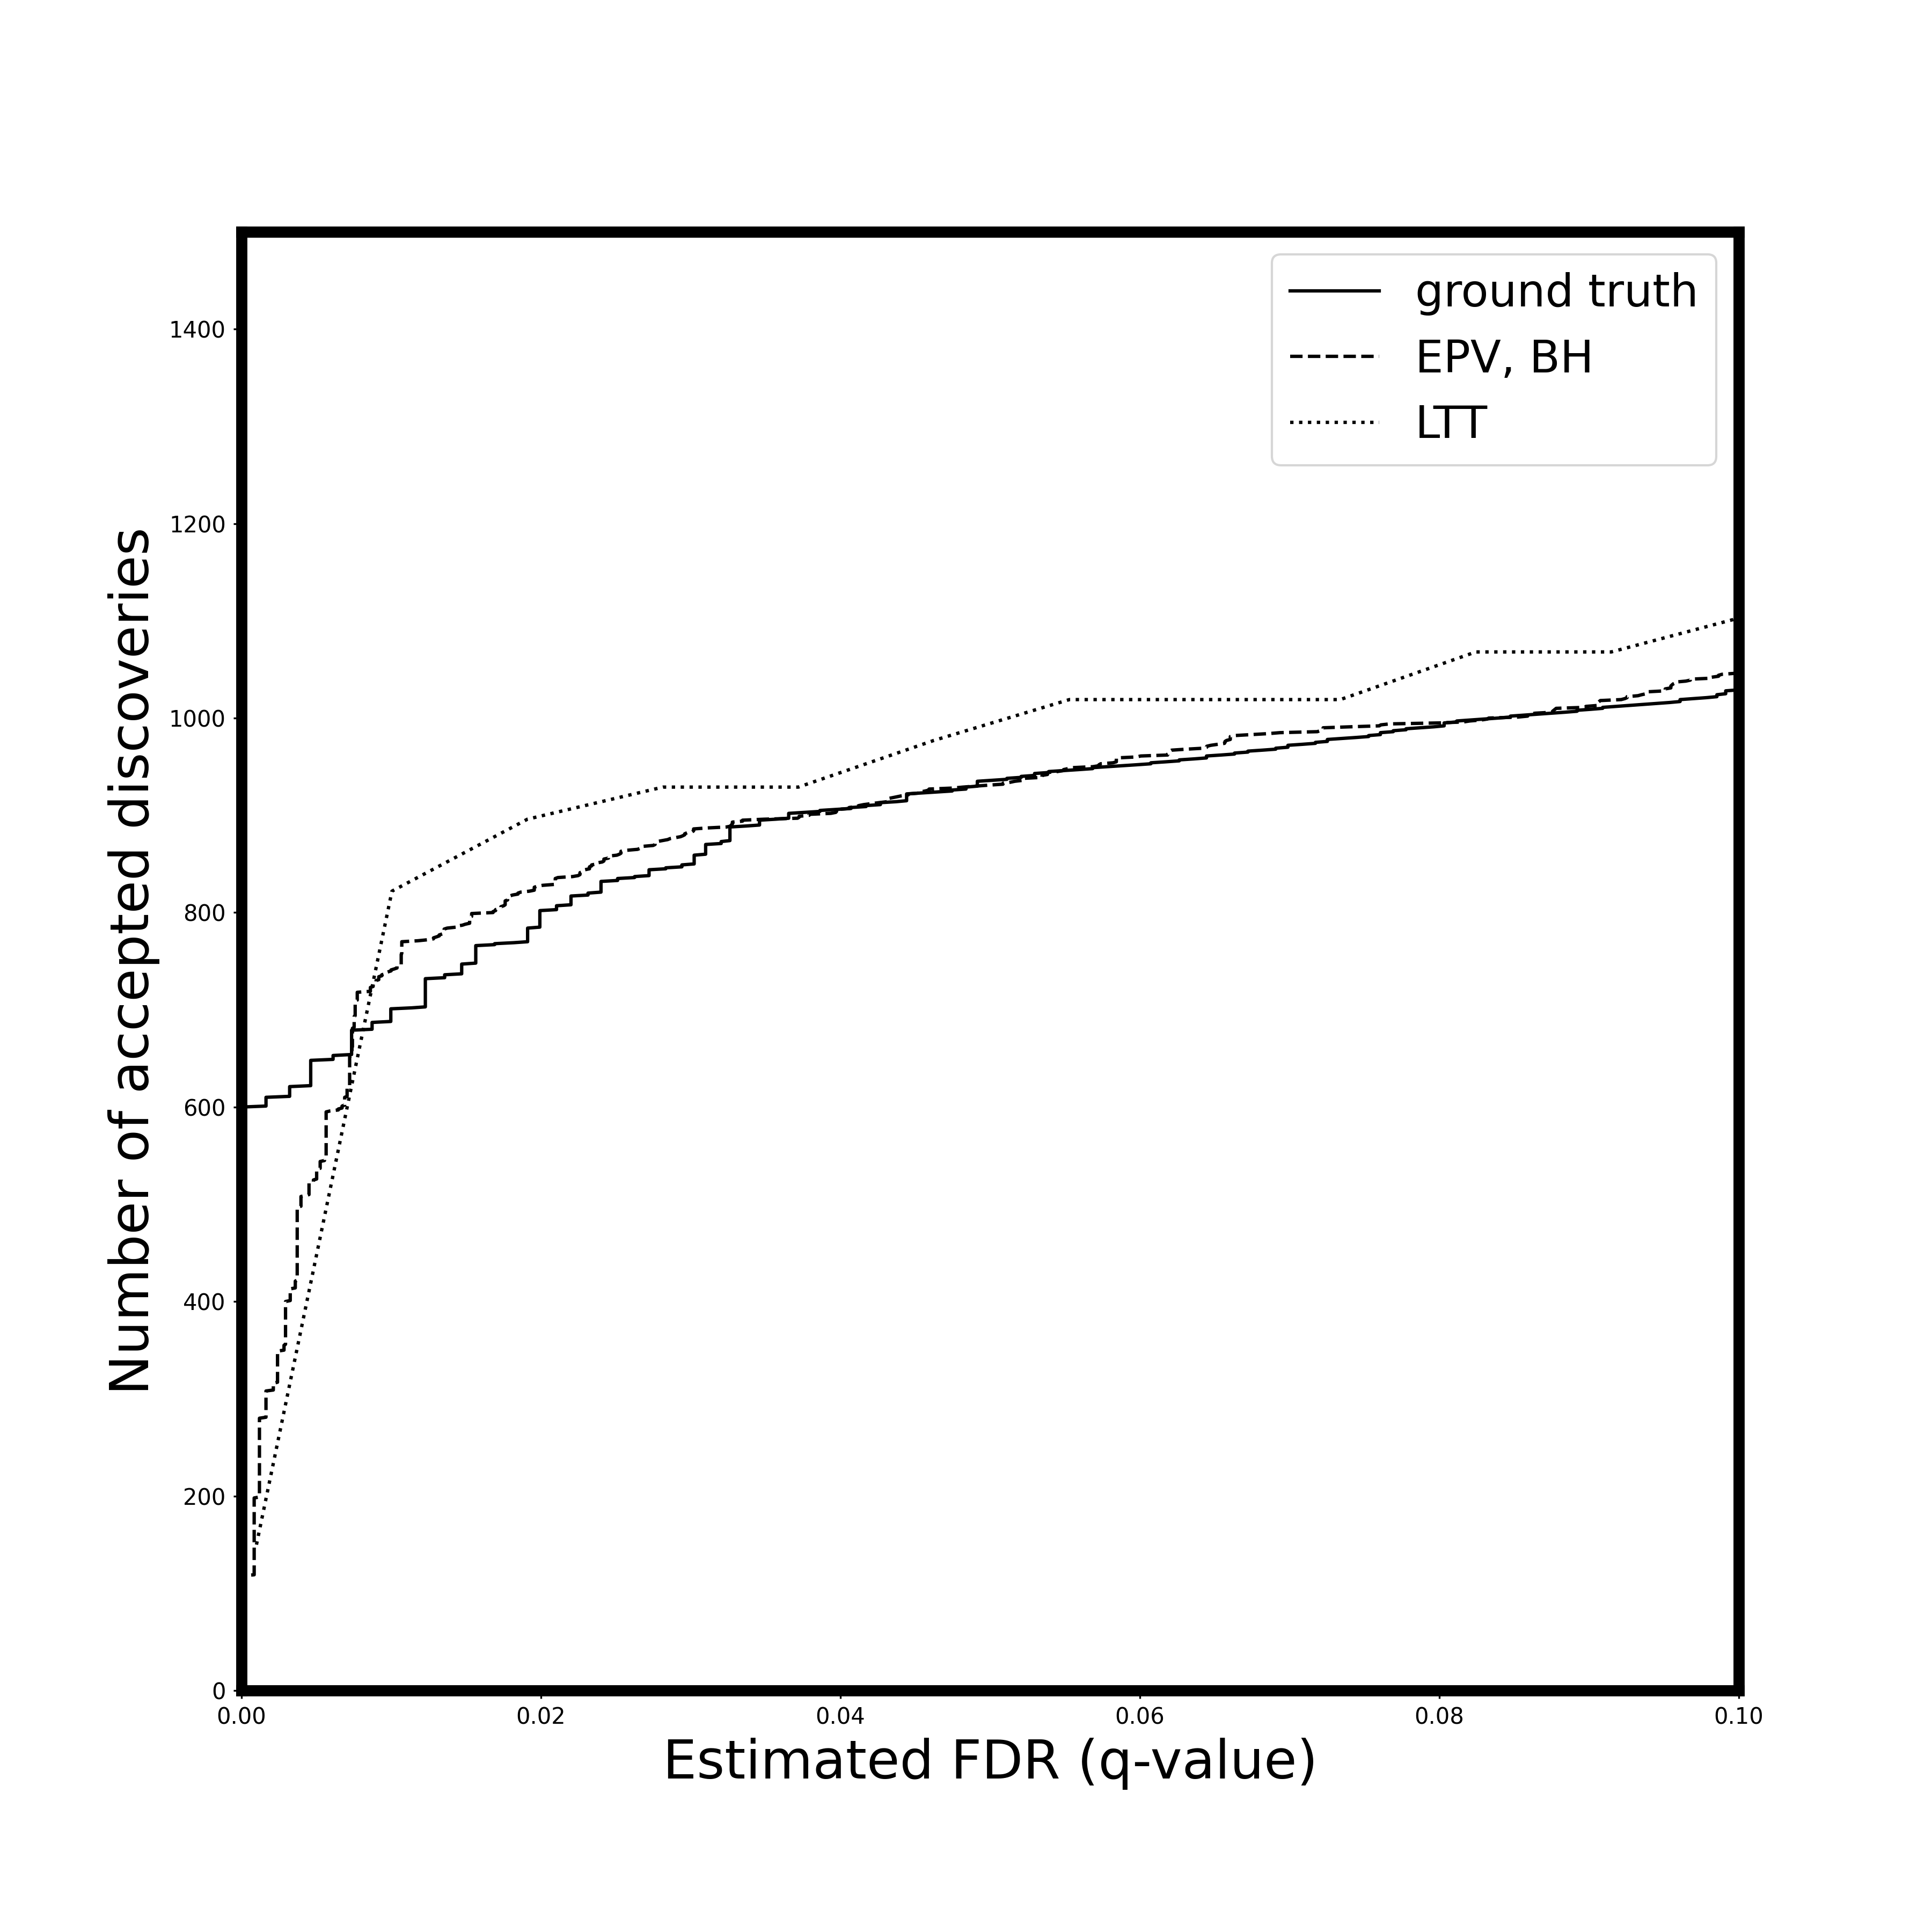
\includegraphics[width=0.225\linewidth, height=0.225\linewidth]{img/cnn_shifted_fdr_control_loc.png} &
		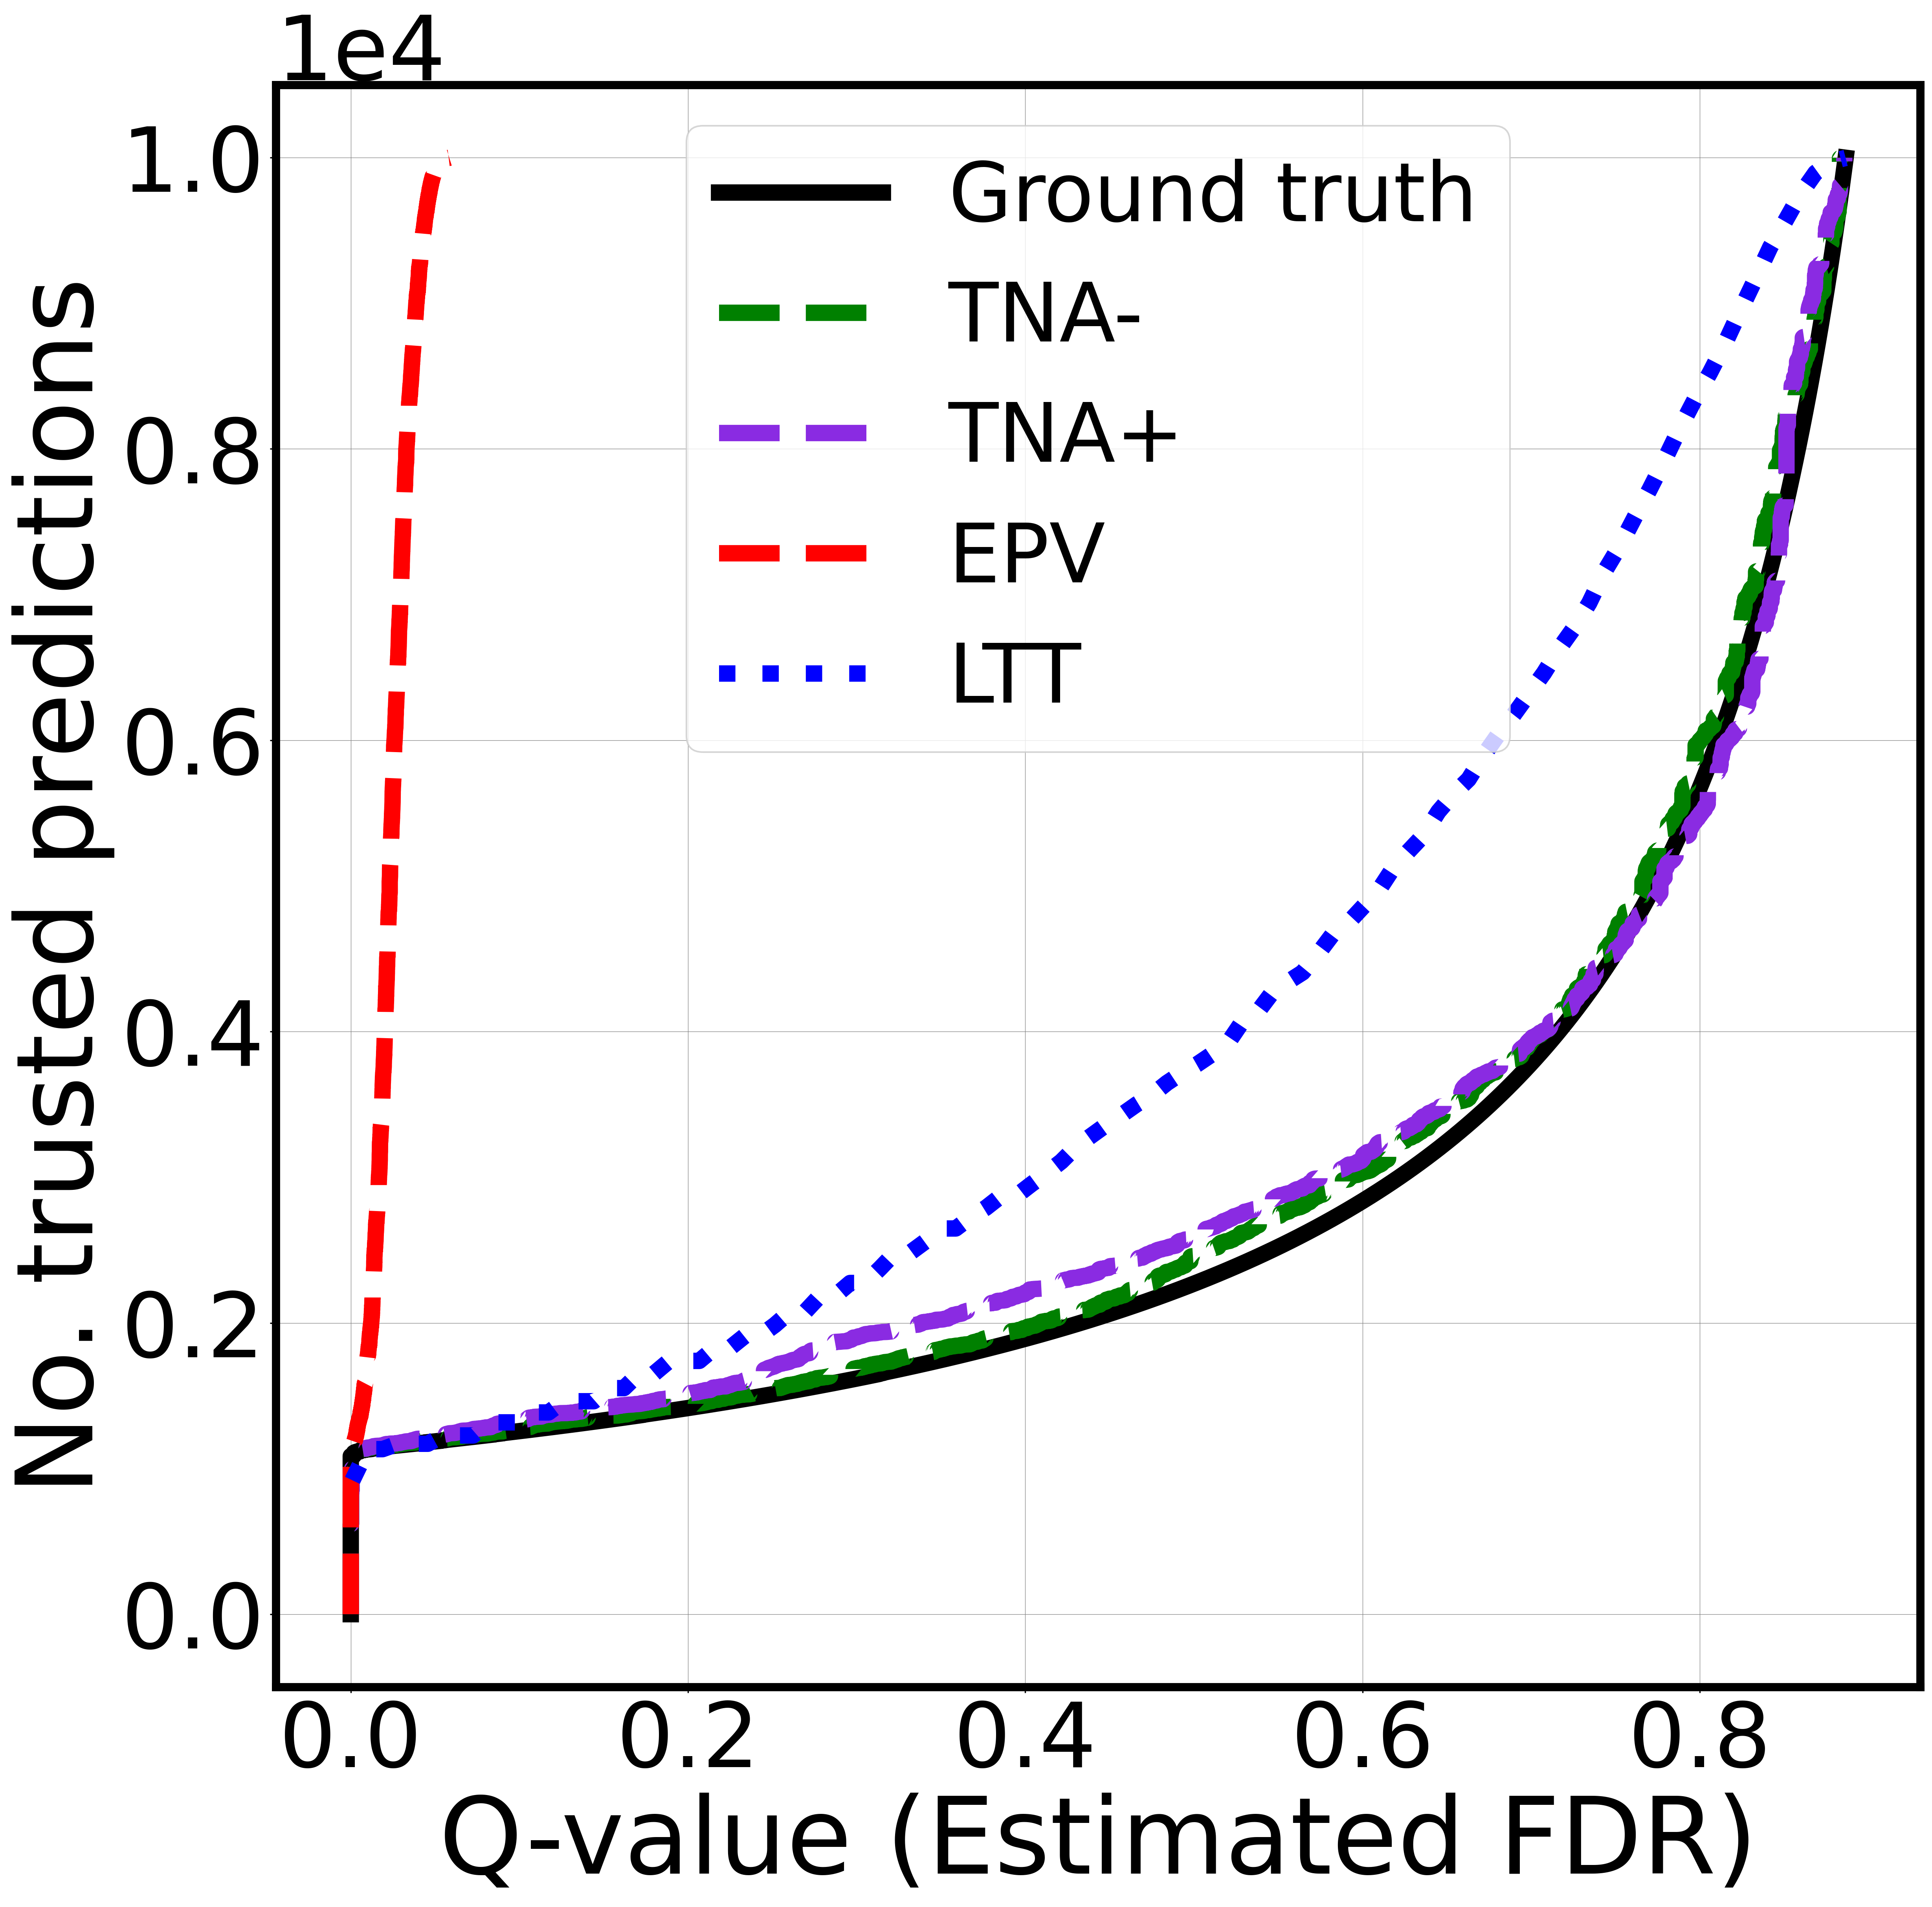
\includegraphics[width=0.225\linewidth, height=0.225\linewidth]{img/cnn_shifted_fdr_control.png} & 
		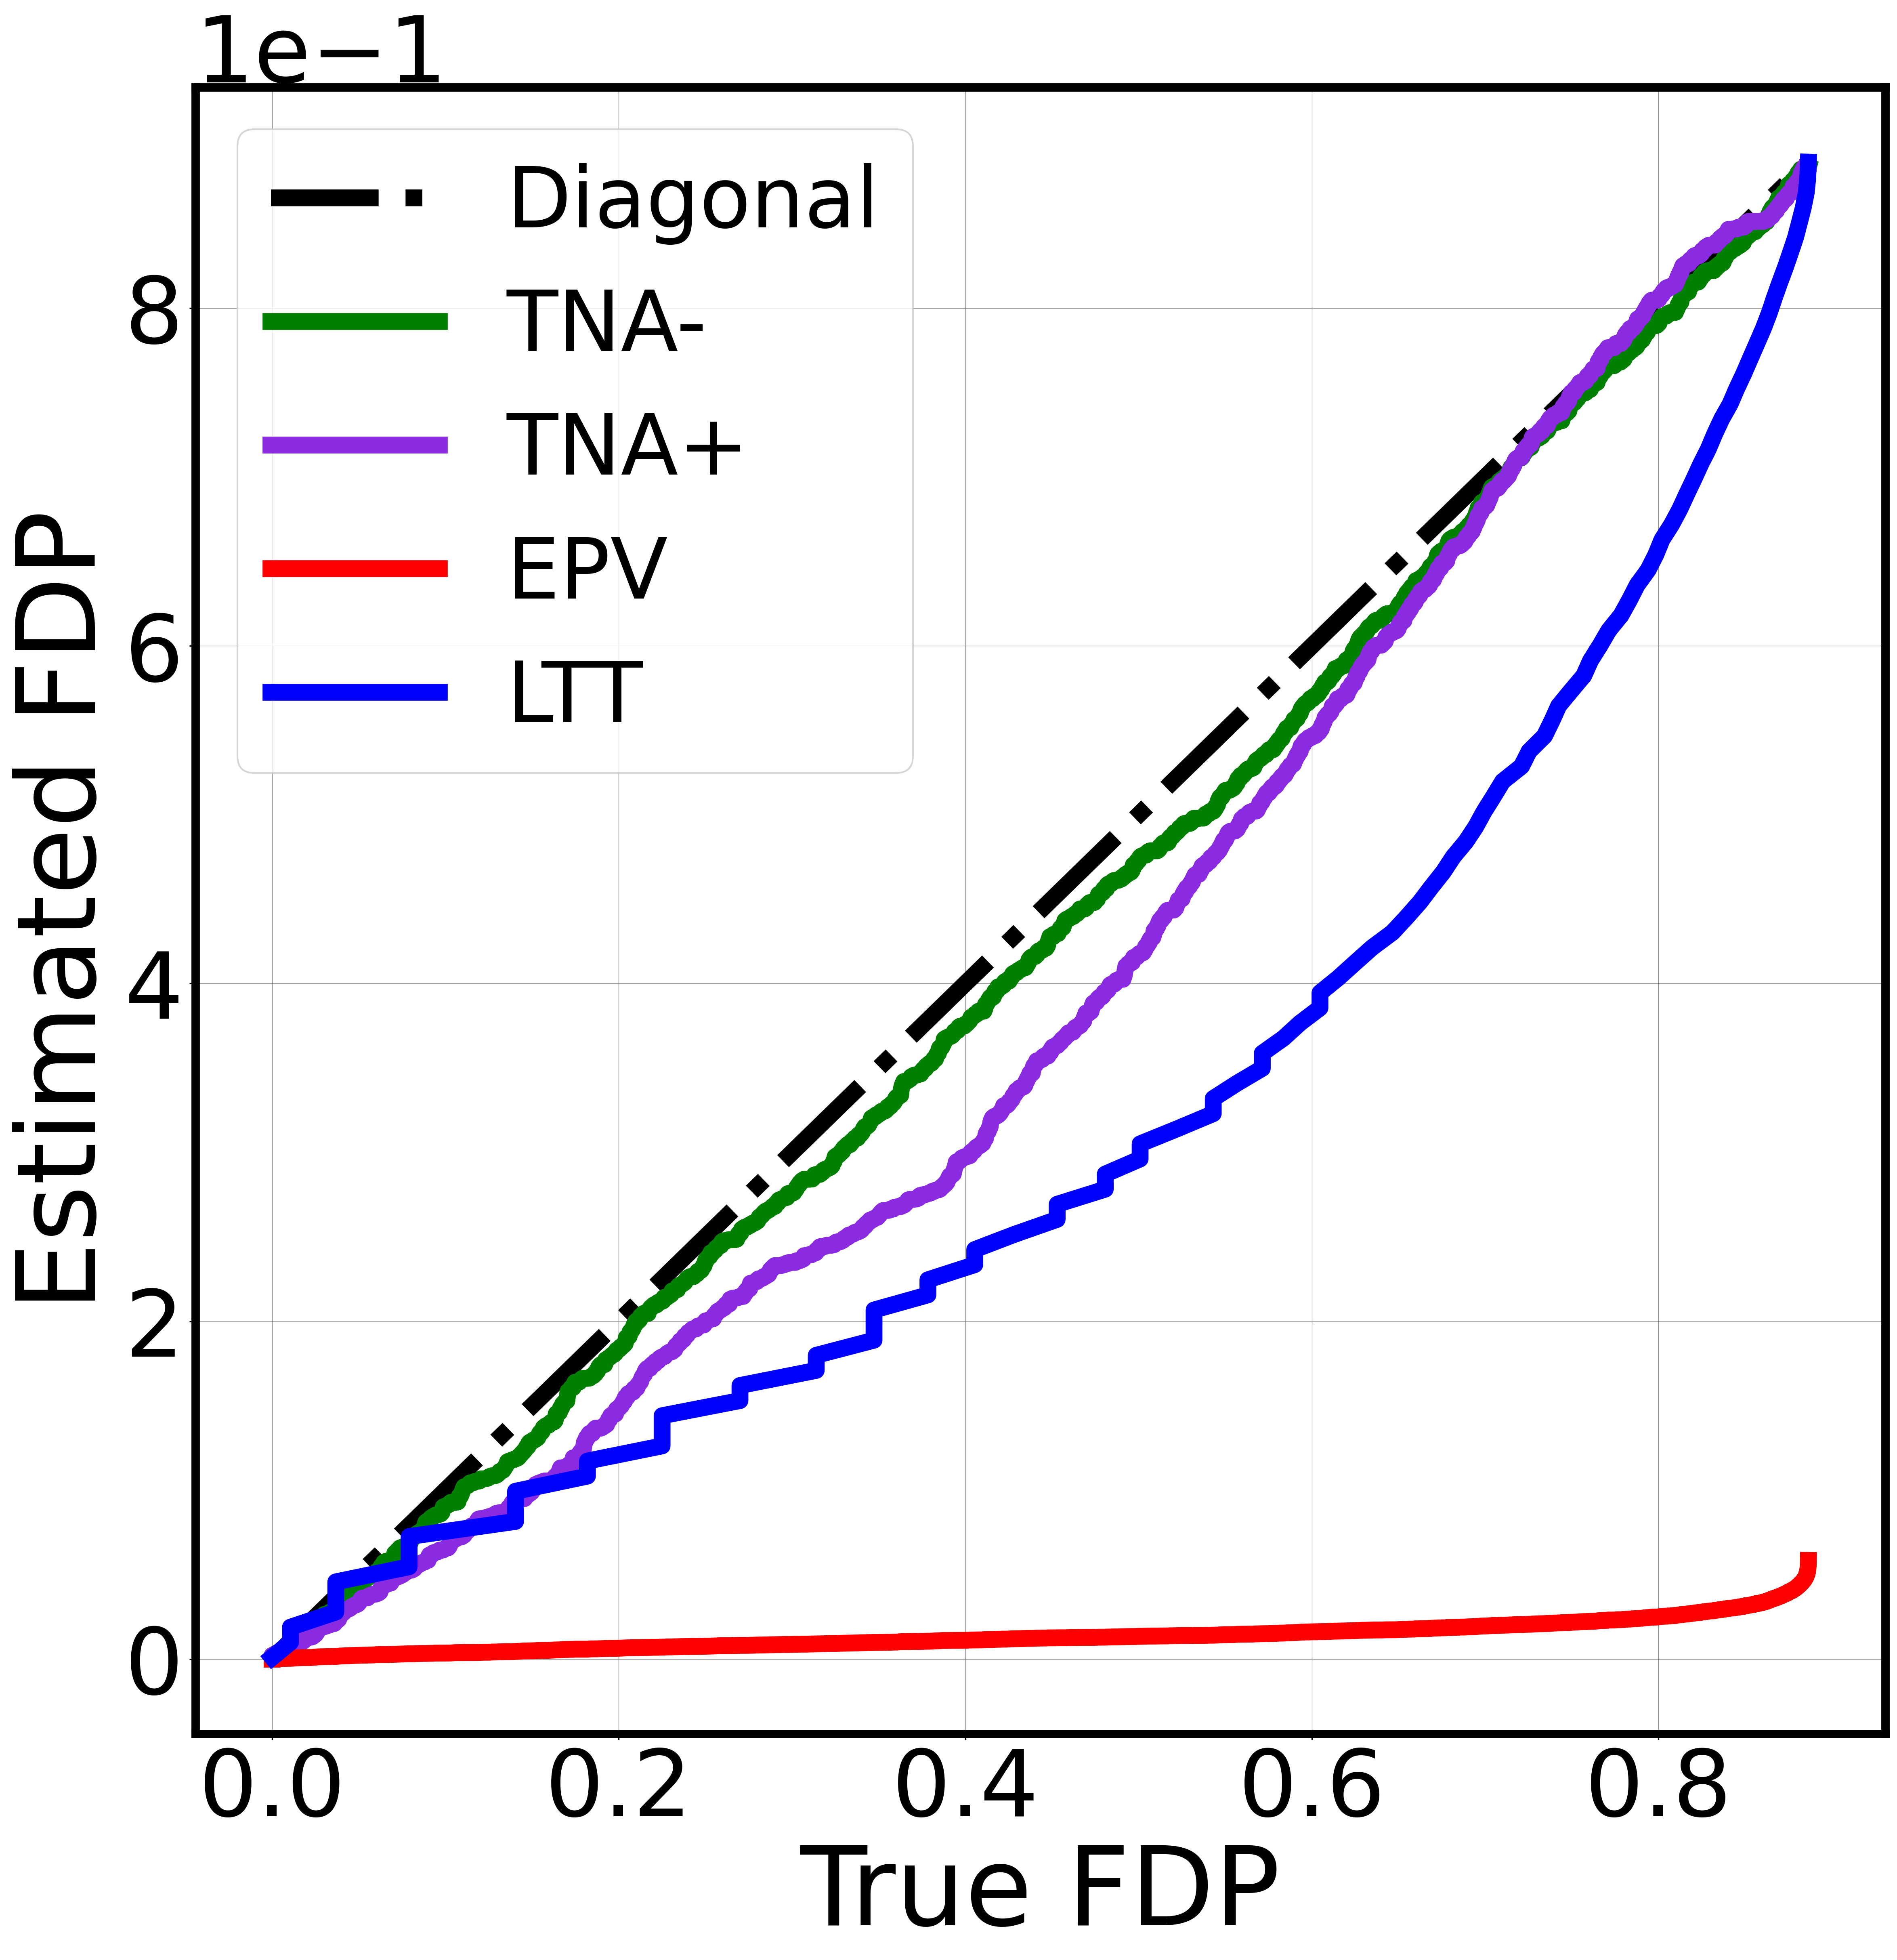
\includegraphics[width=0.225\linewidth, height=0.225\linewidth]{img/cnn_FDPscat_shifted.png} \\
		\multicolumn{4}{l}{\bf (ii) Class distribution shift:}\\
		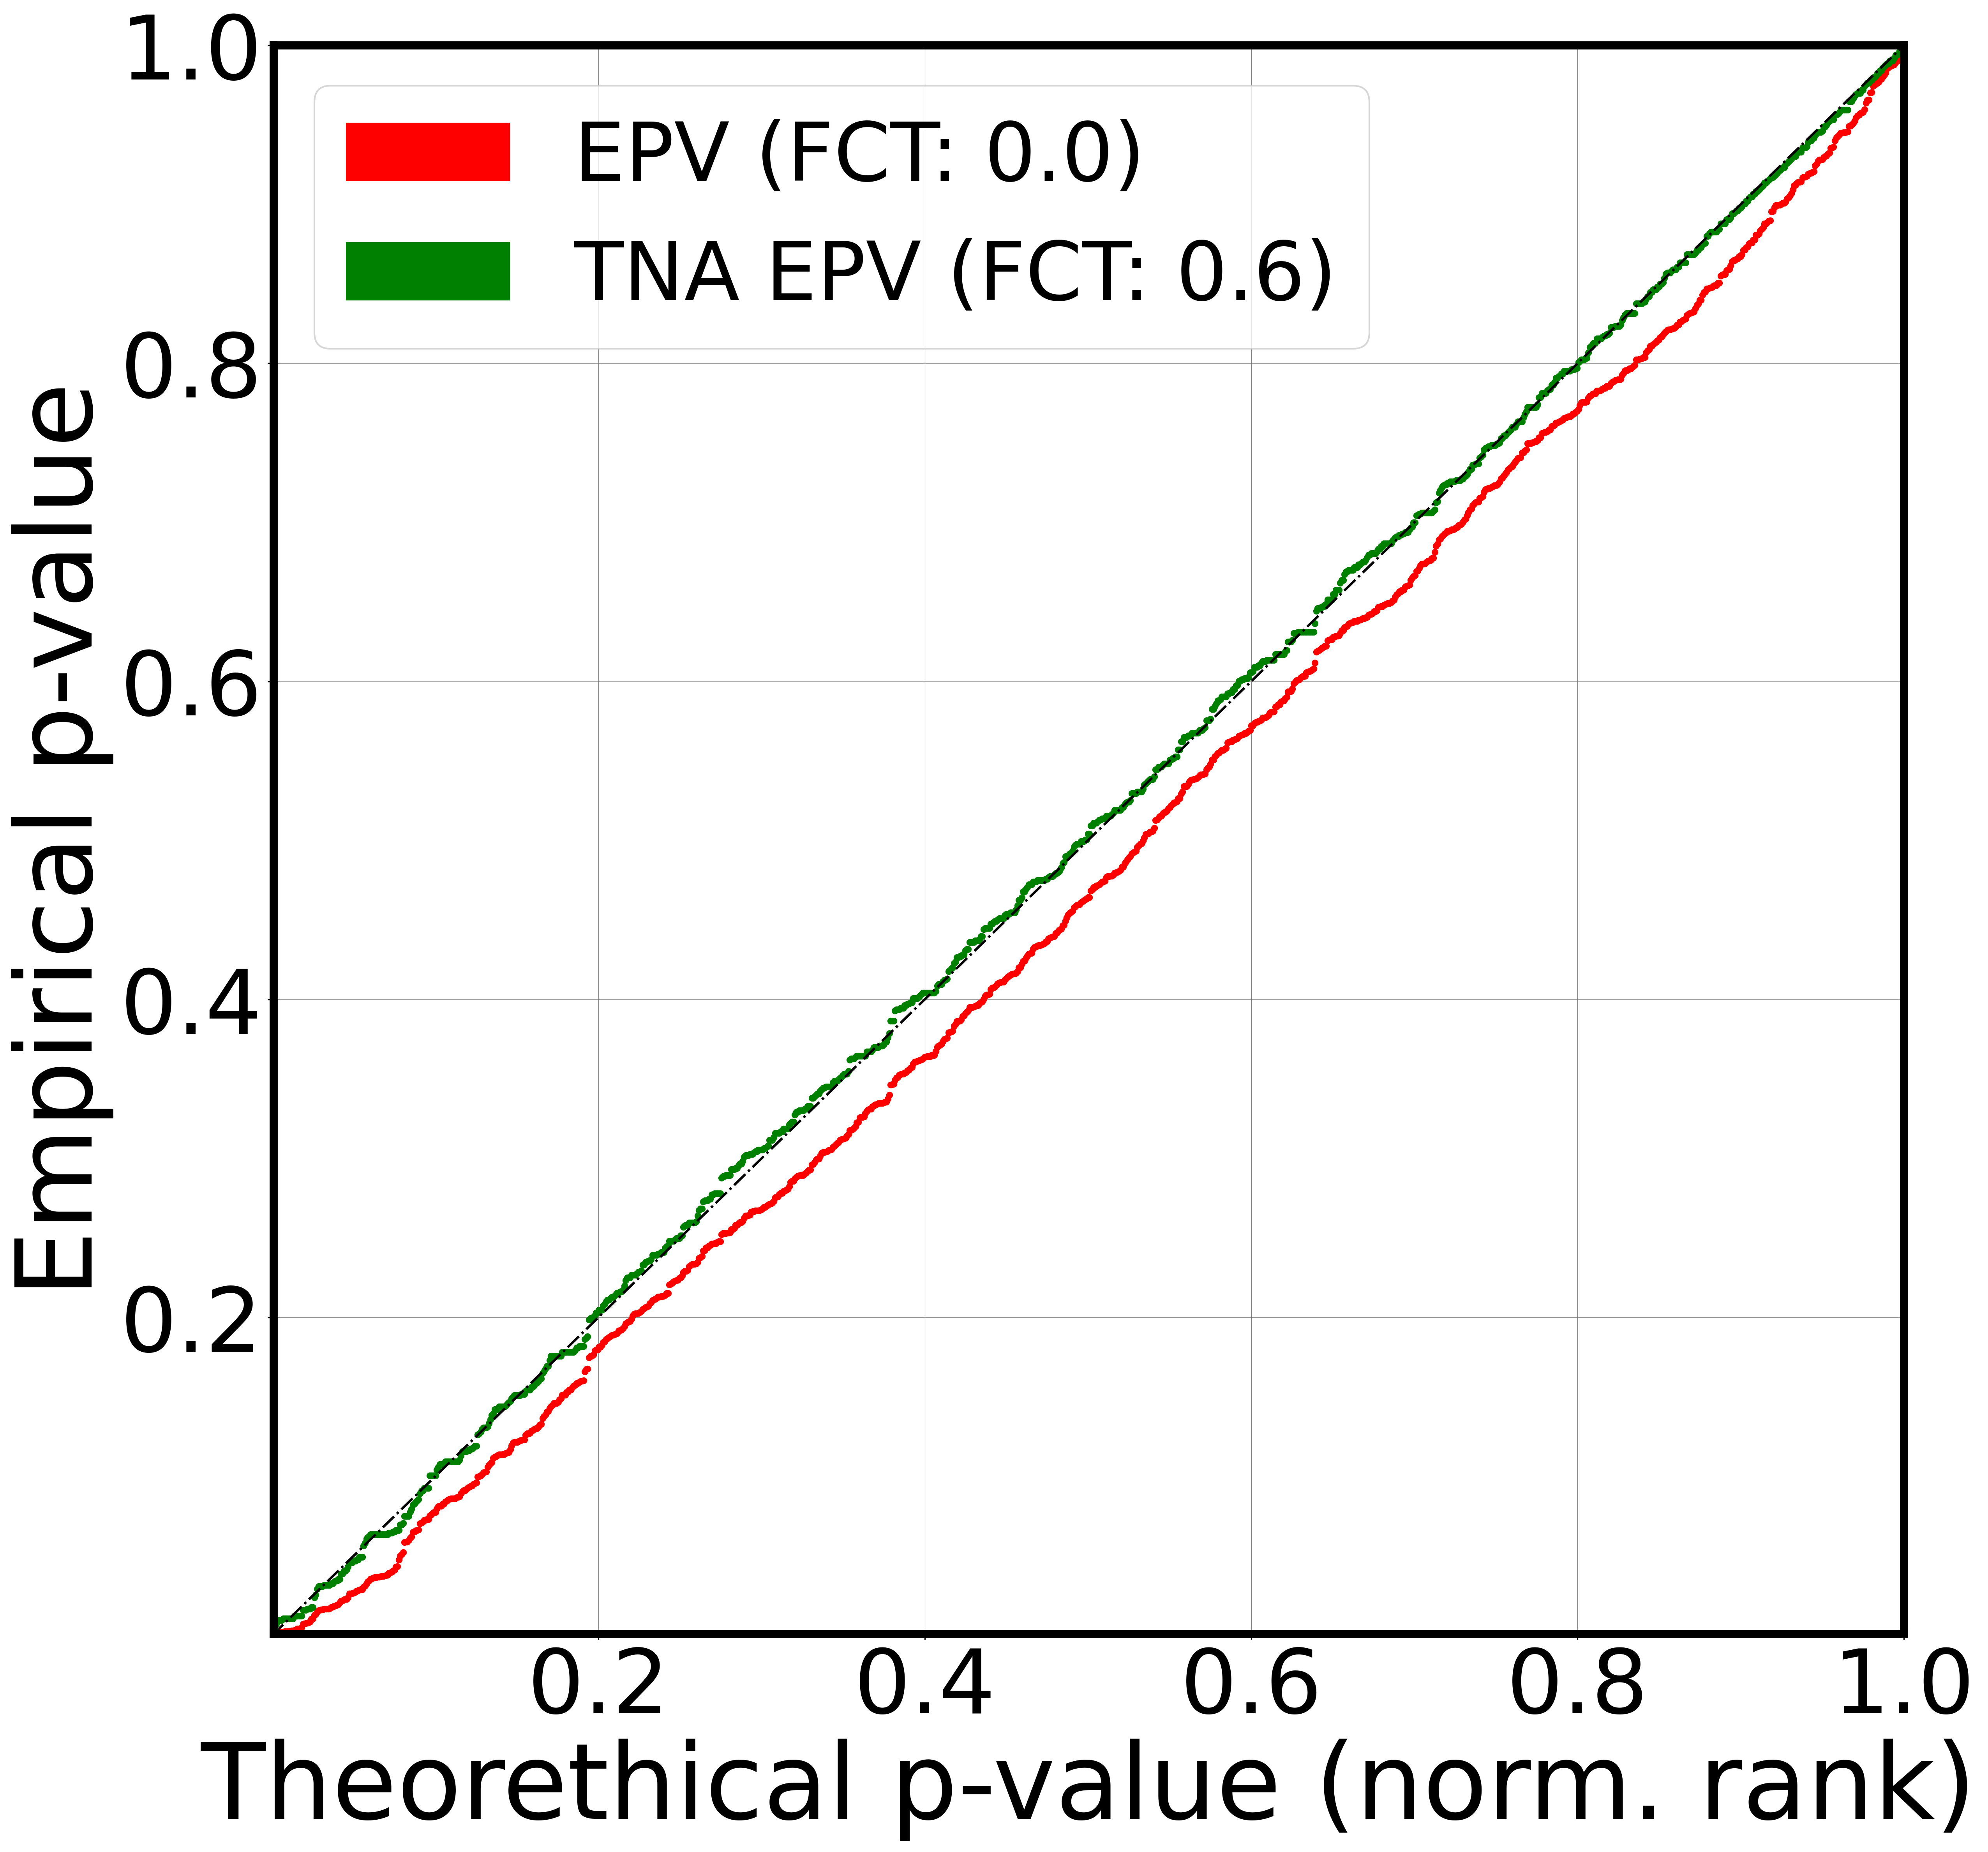
\includegraphics[width=0.225\linewidth, height=0.225\linewidth]{img/cnn_QQ_balanced.png}&
		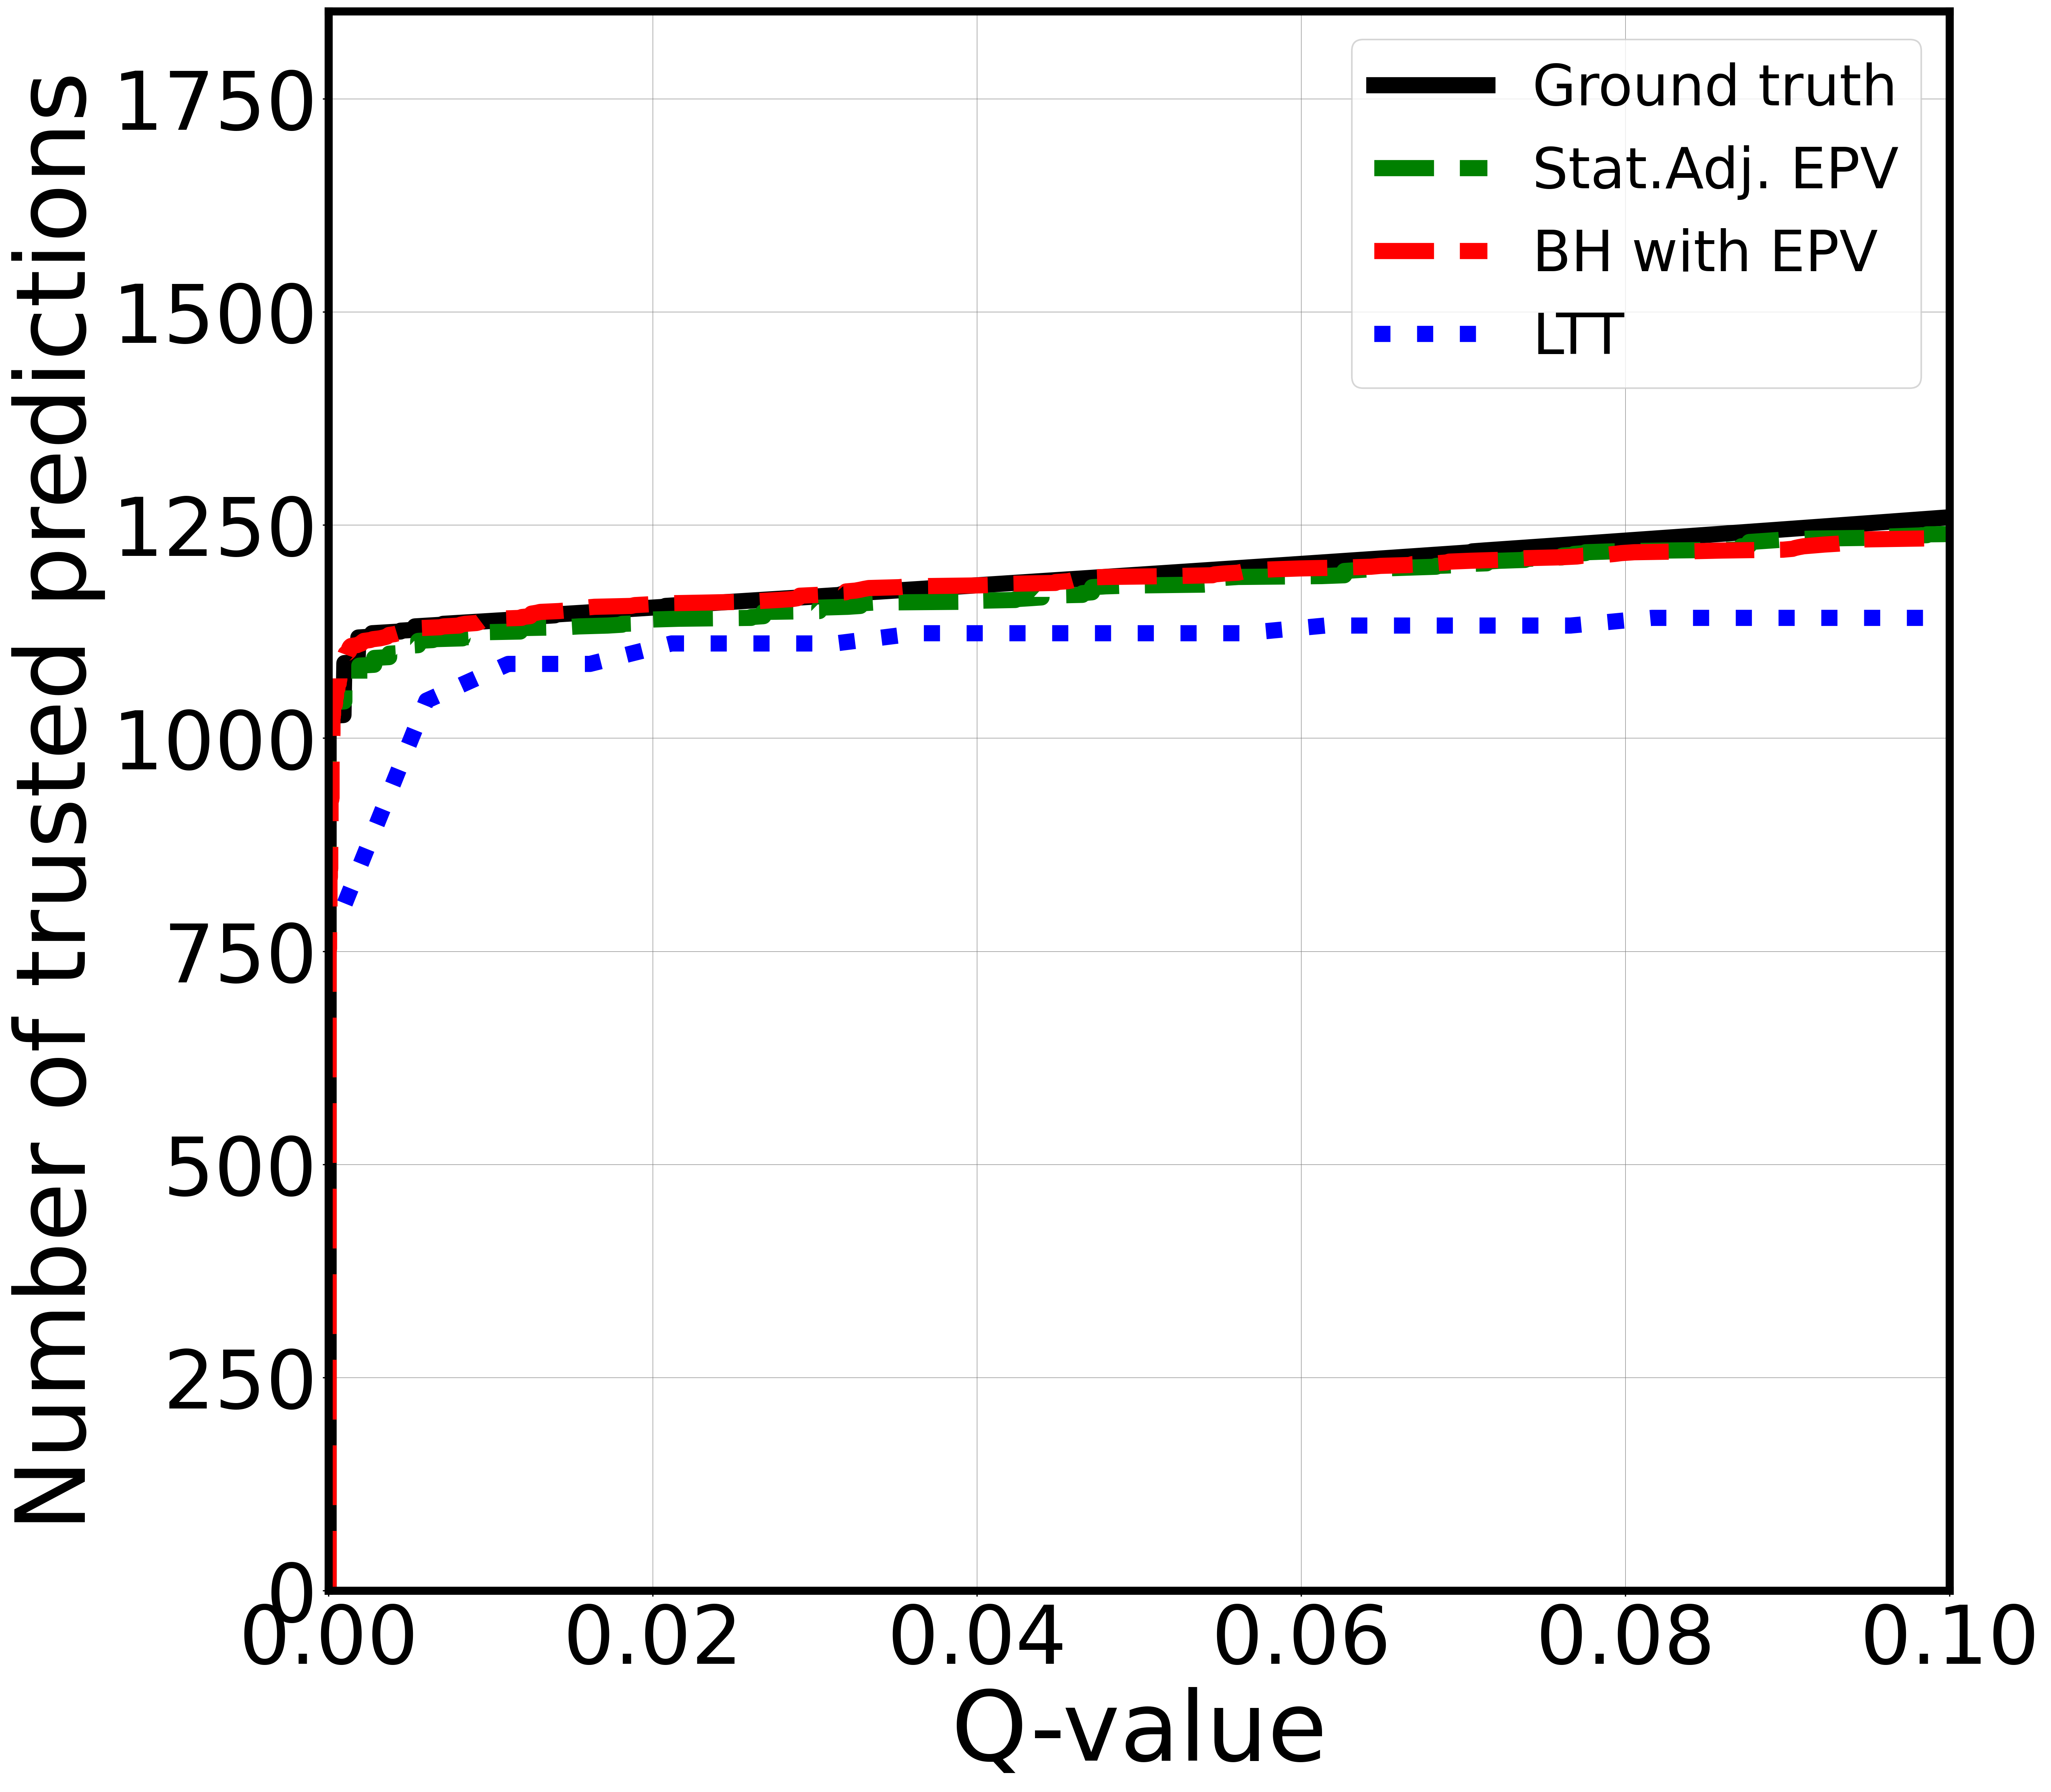
\includegraphics[width=0.225\linewidth, height=0.225\linewidth]{img/cnn_balanced_fdr_control_loc.png} &
		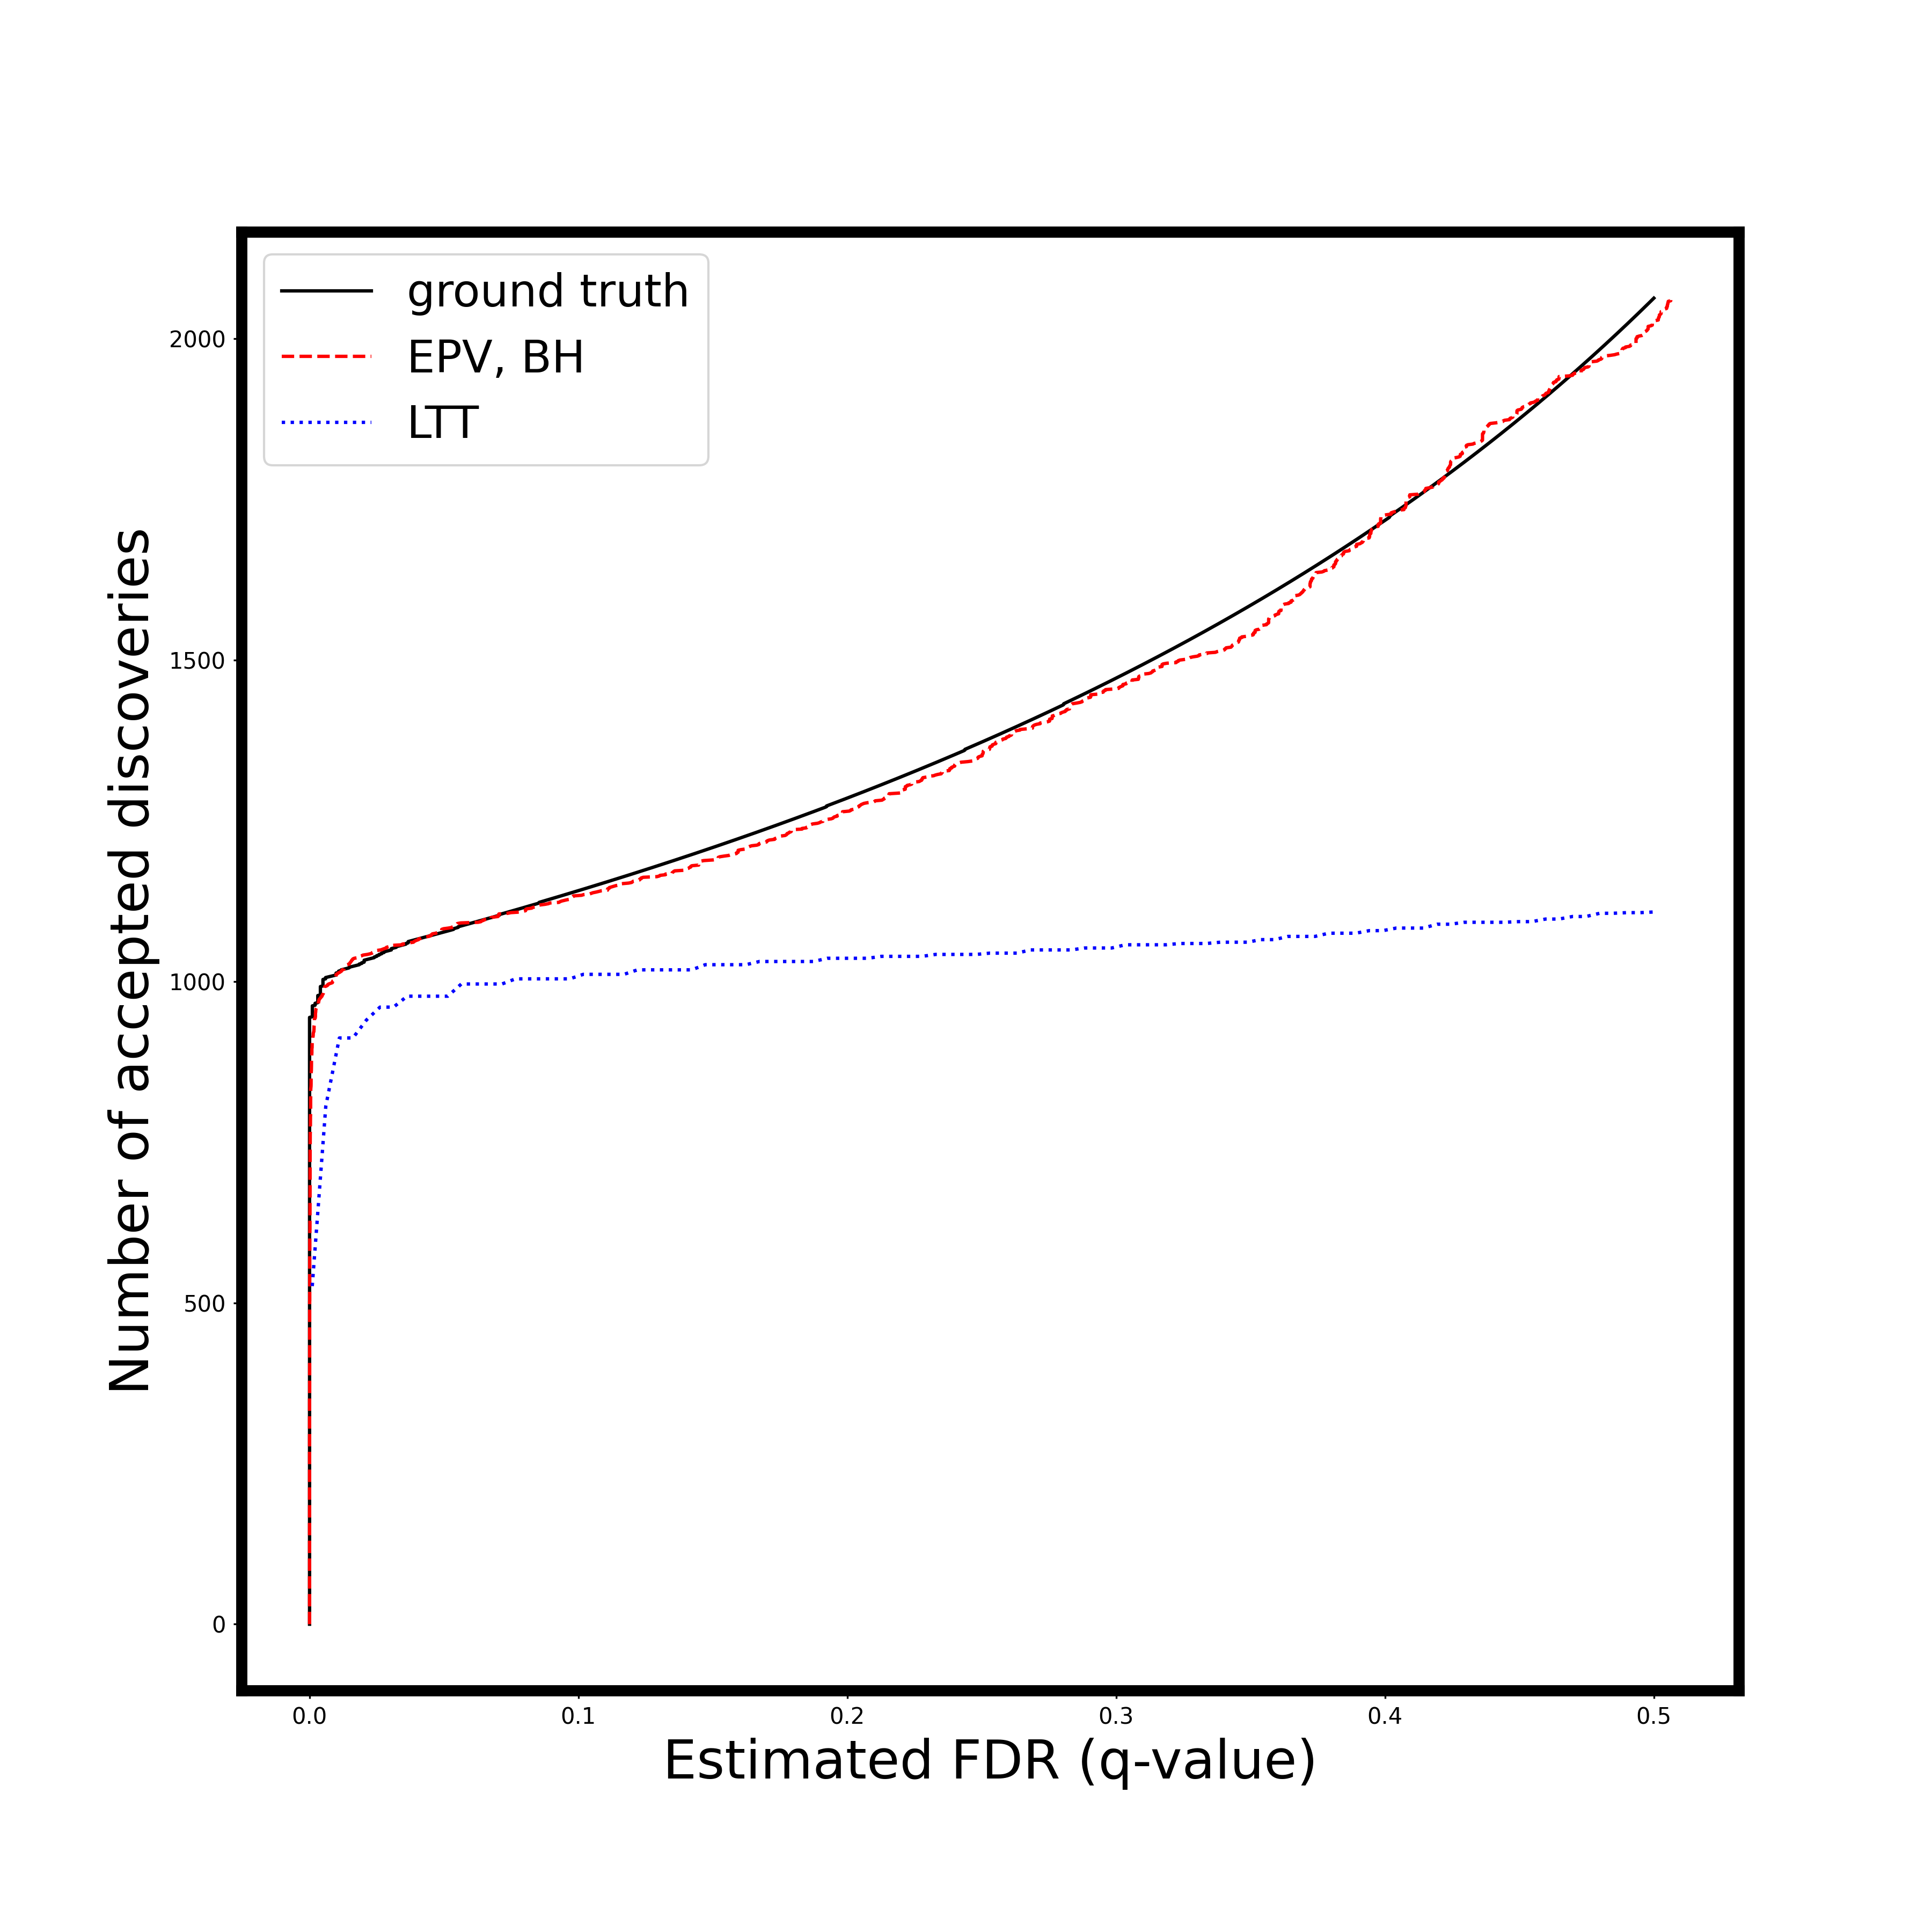
\includegraphics[width=0.225\linewidth, height=0.225\linewidth]{img/cnn_balanced_fdr_control.png} & 
		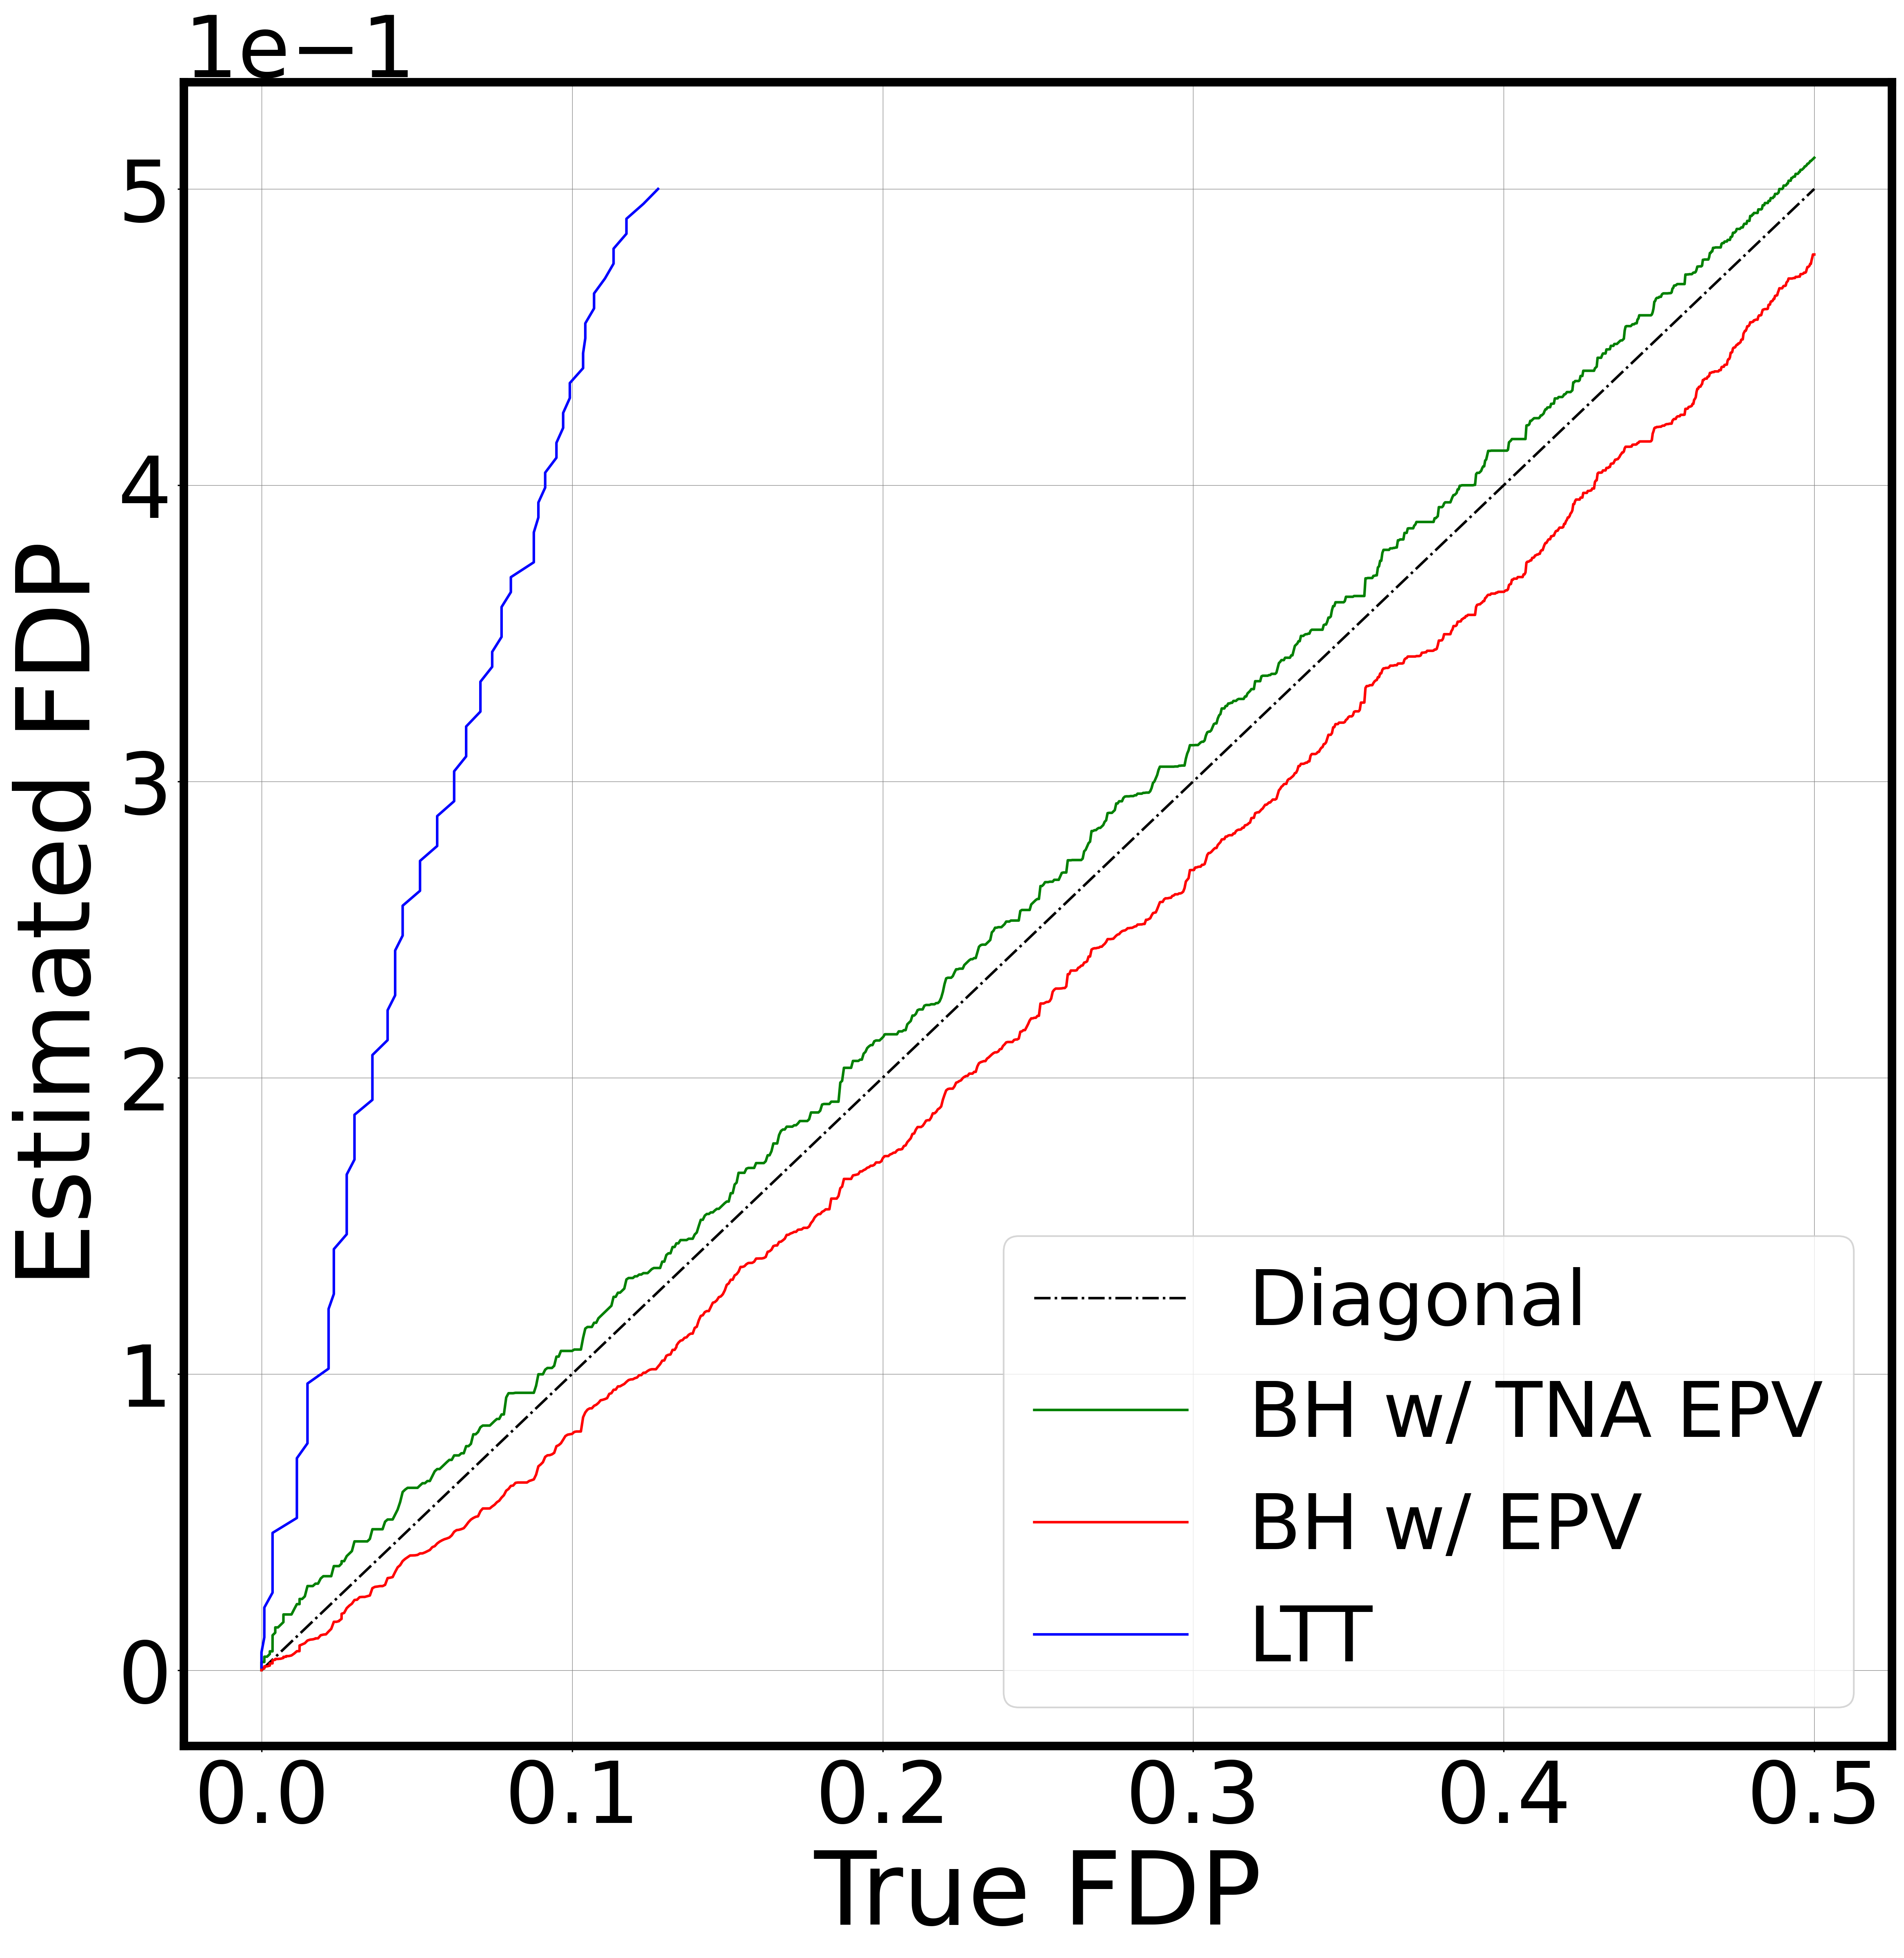
\includegraphics[width=0.225\linewidth, height=0.225\linewidth]{img/cnn_FDPscat_balanced.png} \\		
		A & B & C & D \\
	\end{tabular}
\caption{{\bf  FDR control under data (top row) and label (bottom row) shift.}
	(A) Q-Q plot of the EPVs (red dots), the TNA- EPVs (green dots) and the TNA+ EPVs (purple dots) against the theoretical uniform distribution (normalized rank). (B) The number of accepted classifications as a function of the Q-values over a critical range (0-0.1) obtained with (i) ground truth (black line), (ii) BH with EPV (red), (iii) BH with TNA- EPV (green), (iv) BH with TNA- EPV (purple), and (v) LTT (blue). (C) Same as (B) but over the entire q-value range. (D) Deviation of the estimated FDP from the true FDP obtained with (i) BH with EPV (red line), (ii) BH with TNA- EPV  (green line),  (iii) BH with TNA+ EPV  (purple line), and (iv) LTT (blue line).}
	\label{fig:mnist_shfit}
\end{figure}

	
\paragraph{Example 2.} To illustrate the case of data distribution shift, we down-scaled the pixel intensity by 10\% of the test images in the MNIST dataset (but training images remained the same). The accuracy of the CNN classifier (the same as trained in Example \ref{ex:vanilla}) remained at 99 \%. The evaluation plots are shown in Figure \ref{fig:mnist_shfit}(i). The Q-Q plot (Fig. \ref{fig:mnist_shfit}(i)A) shows that the test EPVs (red) became biased due to data distribution shift; however, both TNA methods can correct the EPVs yielding uniformly distributed p-values (green, purple). The number of accepted predictions ((Fig. \ref{fig:mnist_shfit}(i)BC) obtained with BH with EPVs (red) differs from the ground truth substantially (black line), it became liberally biased. The LTT yielded similar amount of accepted predictions (blue) compared to the ground truth in the critical range of q-values ((Fig. \ref{fig:mnist_shfit}(i)B); however, LTT also becomes liberally biased at lower ranges of q-values ((Fig. \ref{fig:mnist_shfit}(i)C). The number of accepted predictions obtained with BH with both TNA EPVs (green, purple) remained close to the ground truth over both the critical and lower ranges of q-values implying accurate FDR control under data distribution shift. The actual deviation of the estimated FDP from the true FDP is shown in Figure \ref{fig:mnist_shfit}(i)D for each method. The TNA+ is slightly less accurate than TNA- in this test scenario.


\paragraph{Example 3.} The FDR estimation is sensitive to changes in class proportions. To illustrate the case of class distribution shift, we resampled the test data so that the number of true negative and positive instances became equal. This approach was used in other articles, e.g.  \cite{joseph_d__viviano__2019}. The accuracy of the CNN classifier (the same as trained in Example \ref{ex:vanilla}) remained at 99 \%. The evaluation plots are shown in Figure \ref{fig:mnist_shfit}(ii). The Q-Q plot (Fig. \ref{fig:mnist_shfit}(ii)A) shows that the EPVs (red) remained unbiased and so did TNA EPVs (green, purple). This is in  fact expected, because the shift in class distributions should not affect the actual null distributions; Therefore, the results of BH-based methods rely on the $\pi_0$ estimation. BH with EPV and TNA EPV remained accurate and produced results close to the ground truth (red, green, and purple lines in Fig \ref{fig:mnist_shfit}(ii)BCD) indicating successful $\pi_0$ estimation. The BH is robust to changes in class proportions because it can involve the (re-) estimation of the negative data proportion ($\pi_0$) that can be done with, e.g. Storey method. The LTT is also sensitive to changes in class proportions because it relies on the class proportions that are calculated with the training (validation) datasets, and it assumes that class proportions remain unchanged in test phase. Here, LTT resulted in conservative FDR control even at the critical range of q-values (blue in Fig. \ref{fig:mnist_shfit}(ii)BC). The bias in FDR produced by LTT (blue) is also visible in Figure \ref{fig:mnist_shfit}(ii)D. 



%\printbibliography	 
%\bibliographystyle{plain}           % Style BST file.
\bibliographystyle{unsrt}           % Style BST file.
\bibliography{bibliography}

\section*{Author contributions}
\ifdefined\DOUBLEBLINDREVIEW
Omitted for double-blind peer-review.
\else
AKF concieved the idea and supervised the project,  AB worked out the methods and carried out experiments. AKF and AB wrote the manuscript.
\fi 
\section*{Data availability}
The data used in this study are secondary data obtained from publicly available sources. All data sources are properly cited within the manuscript. No new primary data were generated or analyzed in this research. For access to the datasets used, please refer to the original sources as indicated in the references section.

\section*{Additional information}
The authors declare no conflicts of interest.


\end{document}


\section{Experimental results}

\subsection{PCam: tumor classification}



The PatchCamelyon (PCam) benchmark dataset is a collection of histopathologic scans of lymph node sections \cite{Veeling2018-qh} derived from the Camelyon 16 challenge \cite{camelyon16}. PCam consists of 327,680 colored images of size 96x96 each. The challenge is to identify the presence (positive) or absence (negative) of any histopathology in one image. The dataset creators of PCam underline that all the positive and negative instances in the training, validation, test sets are equally distributed, resulting in a class balance of 1:1. We used the pre-trained resnet34-pcam model, which is a popular, deep residual network from the TIA (Tissue Image Analysis) toolbox \cite{Pocock2022} with an overall f1-score of 0.889, as stated by the authors. We evaluated the uniformity of the p-values of the test samples and the performance of the FDR controlling methods. The results are shown in the first row of Figure \ref{fig:I}.  The Q-Q plots (Fig. \ref{fig:I}-(i)-A) of the test EPVs (red dots) indicate that the test p-values are slightly biased, possibly indicating a slight overfitting and/or distribution shift between the training and test datasets. However, the Q-Q plots of the test  EPVs adjusted with TNA- (green dots) and TNA+ (purple dots) show a more uniformly distributed p-values. The plots on Fig. \ref{fig:I}-(i)-BCD indicate that all four FDR control methods are mostly accurate with this dataset especially at critical $\alpha$ levels (0-0.1), despite the small bias in the EPVs. The TNA methods (both, TNA- and TNA+) manage to reduce the bias from EPVs and yield more accurate FDR control with BH (green and purple lines), than the BH method with the original EPVs (red line). However, LTT outperformed both BH-based methods in this benchmark. 


\begin{figure}[h!]
	\centering
	\begin{tabular}{cccc}
		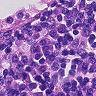
\includegraphics[width=1.in]{img/pcam1.jpg} &
		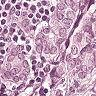
\includegraphics[width=1.in]{img/pcam2.jpg} & 
		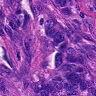
\includegraphics[width=1.in]{img/pcam3.jpg} &
		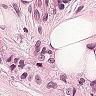
\includegraphics[width=1.in]{img/pcam4.jpg}
	\end{tabular}
	\caption{{\bf Instances of PCam dataset.}}
	\label{fig:pcam_example}
\end{figure} 
 
In our opinion, the actual class proportions in real-life applications can be significantly different from 1:1, making the FDR control with methods like LTT inaccurate in practical applications. We manually resampled the test data so that  the positive and negative class balance became 31\%:69\%, following the original class balance of the Camelyon 16 dataset. The evaluation plots are shown in the second row of Figure \ref{fig:I}. The Q-Q plot (Fig. \ref{fig:I}-(ii)-A) reveals that the EPVs (red dots) become slightly biased; however, our TNA methods manage to reduce this bias from the EPVs (green dots). The LTT method became liberal in FDR control, the BH protocol with standard EPVs resulted in conservative FDR control; whereas, the BH with the TNA EPVs remained accurate, especially at critical range of q-values (0-0.1) (Fig. \ref{fig:I}-(ii)-C).




\begin{figure}[h!]
	
	\begin{tabular}{cccc}
		\multicolumn{4}{l}{\bf (i) Standard PCam dataset:}\\		
		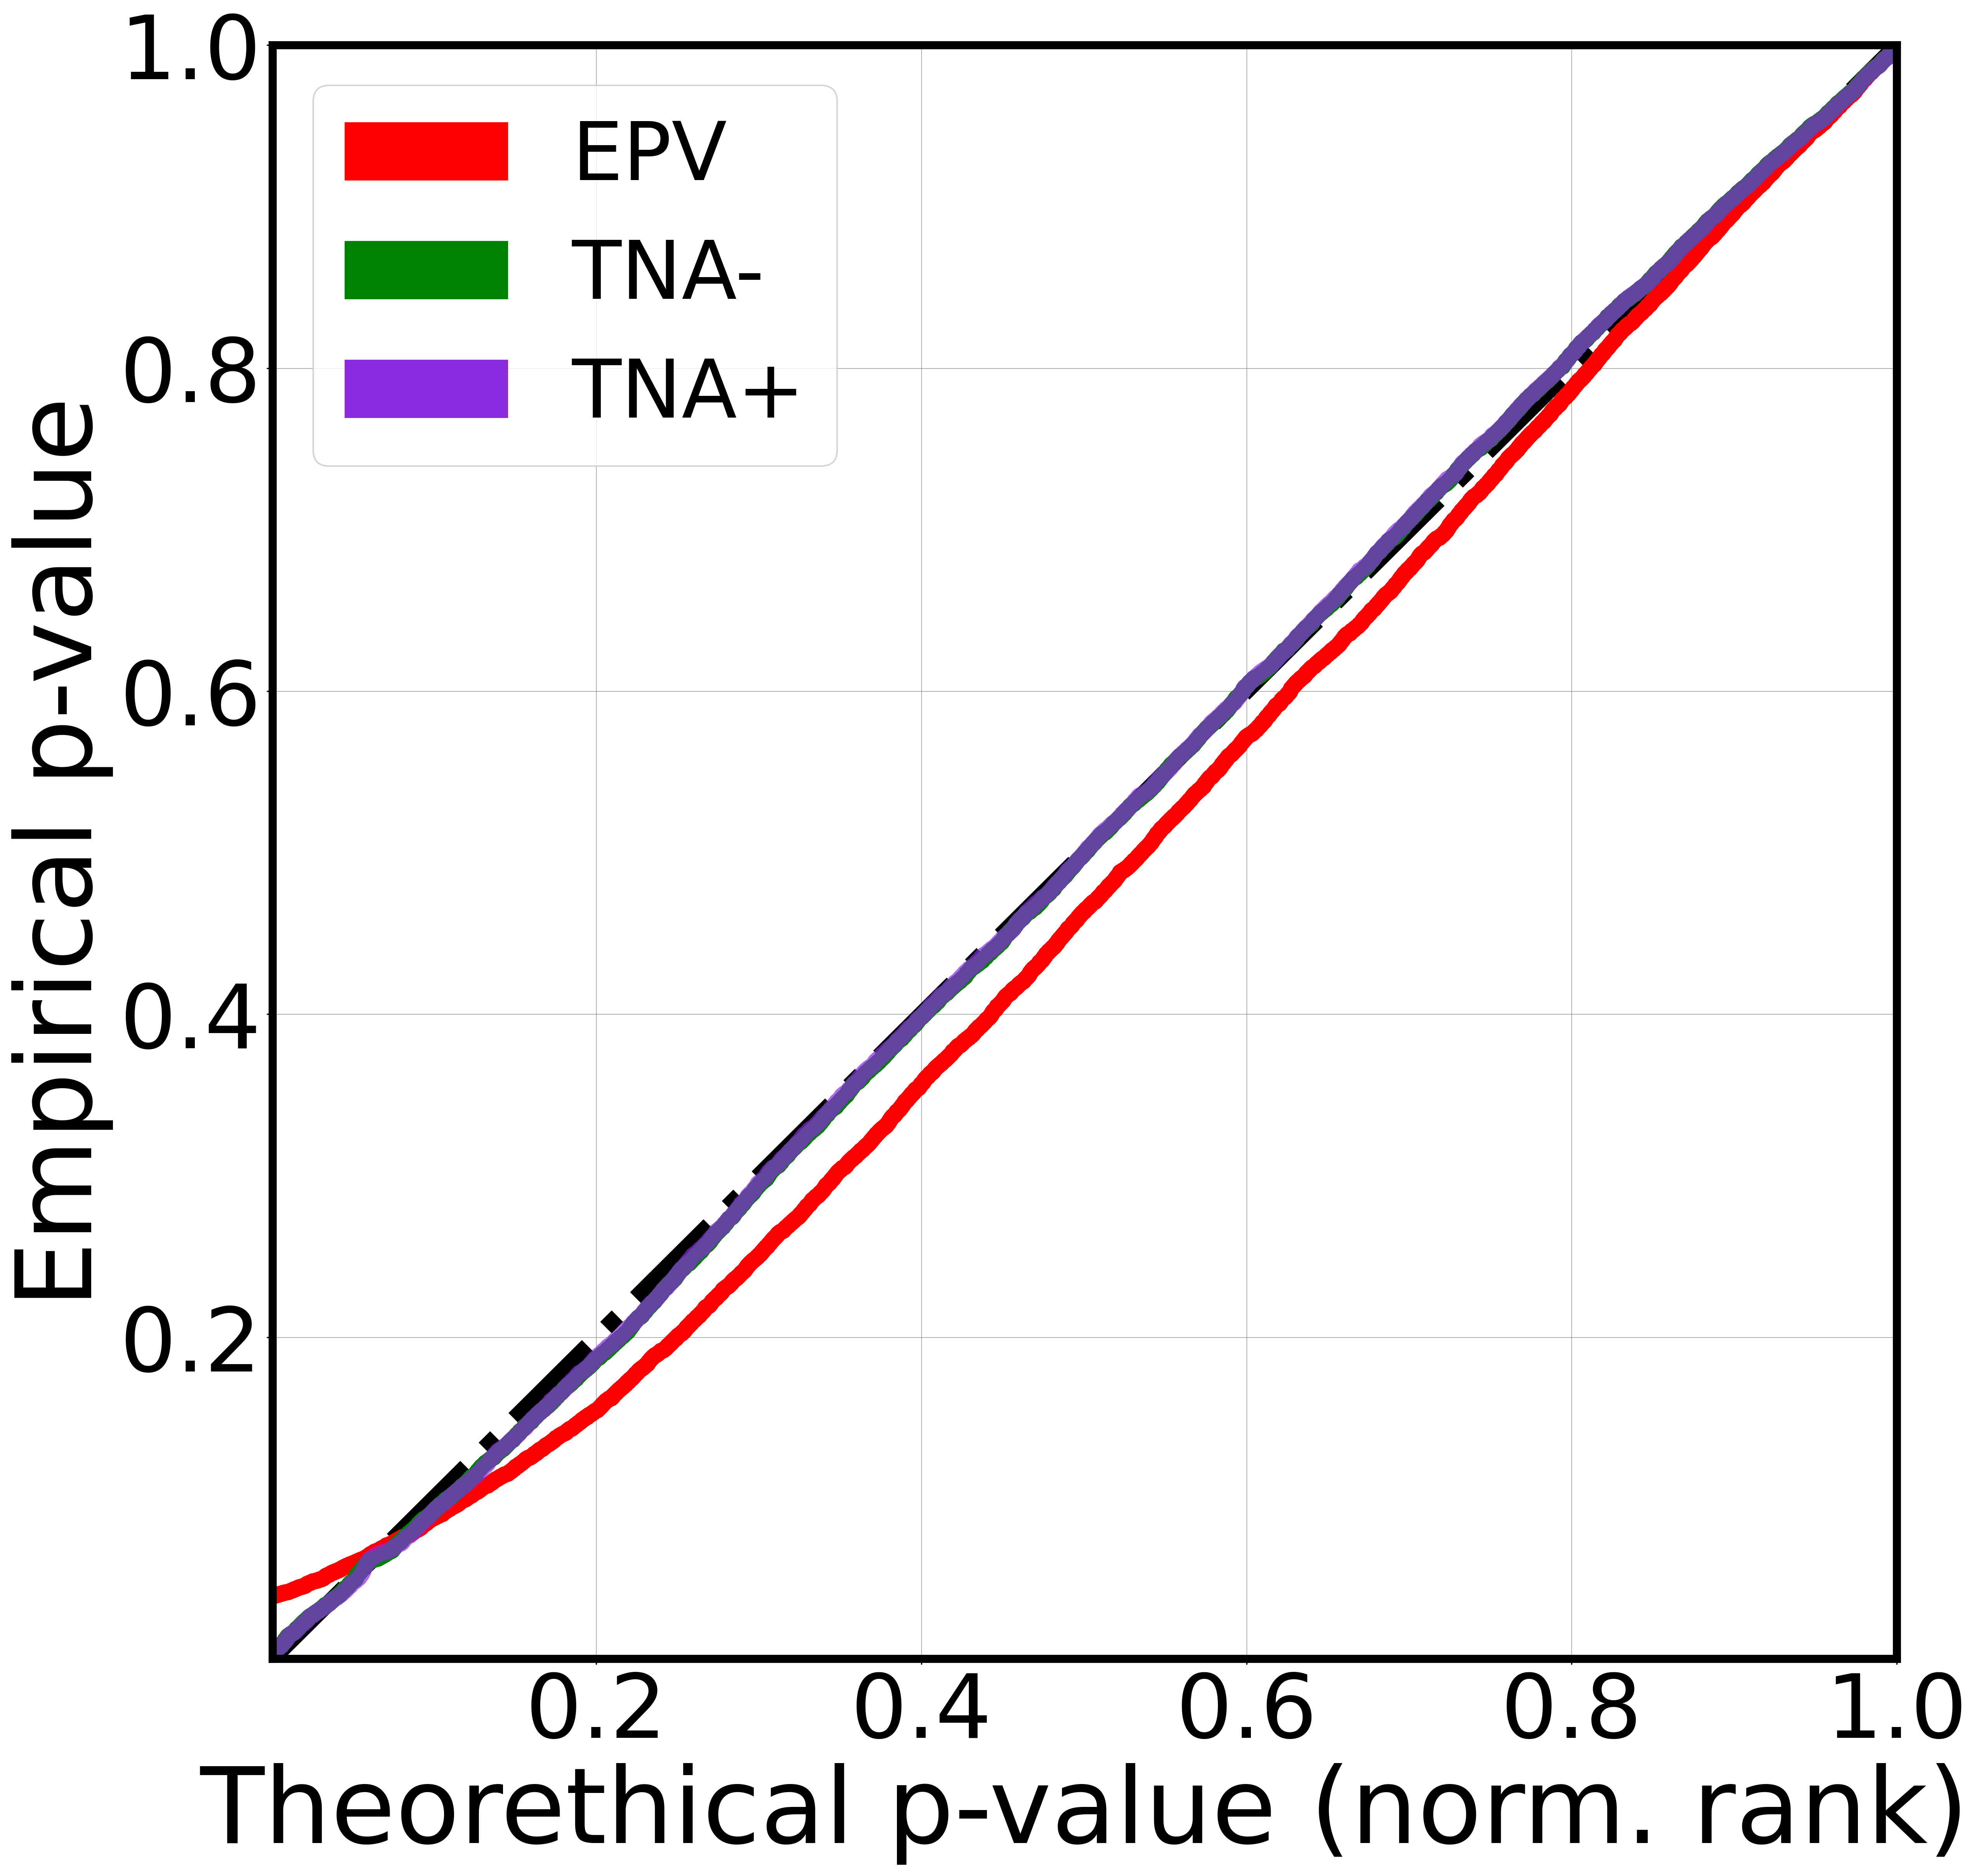
\includegraphics[width=0.225\linewidth, height=0.225\linewidth]{img/cnn_QQ_pcam.png} &
		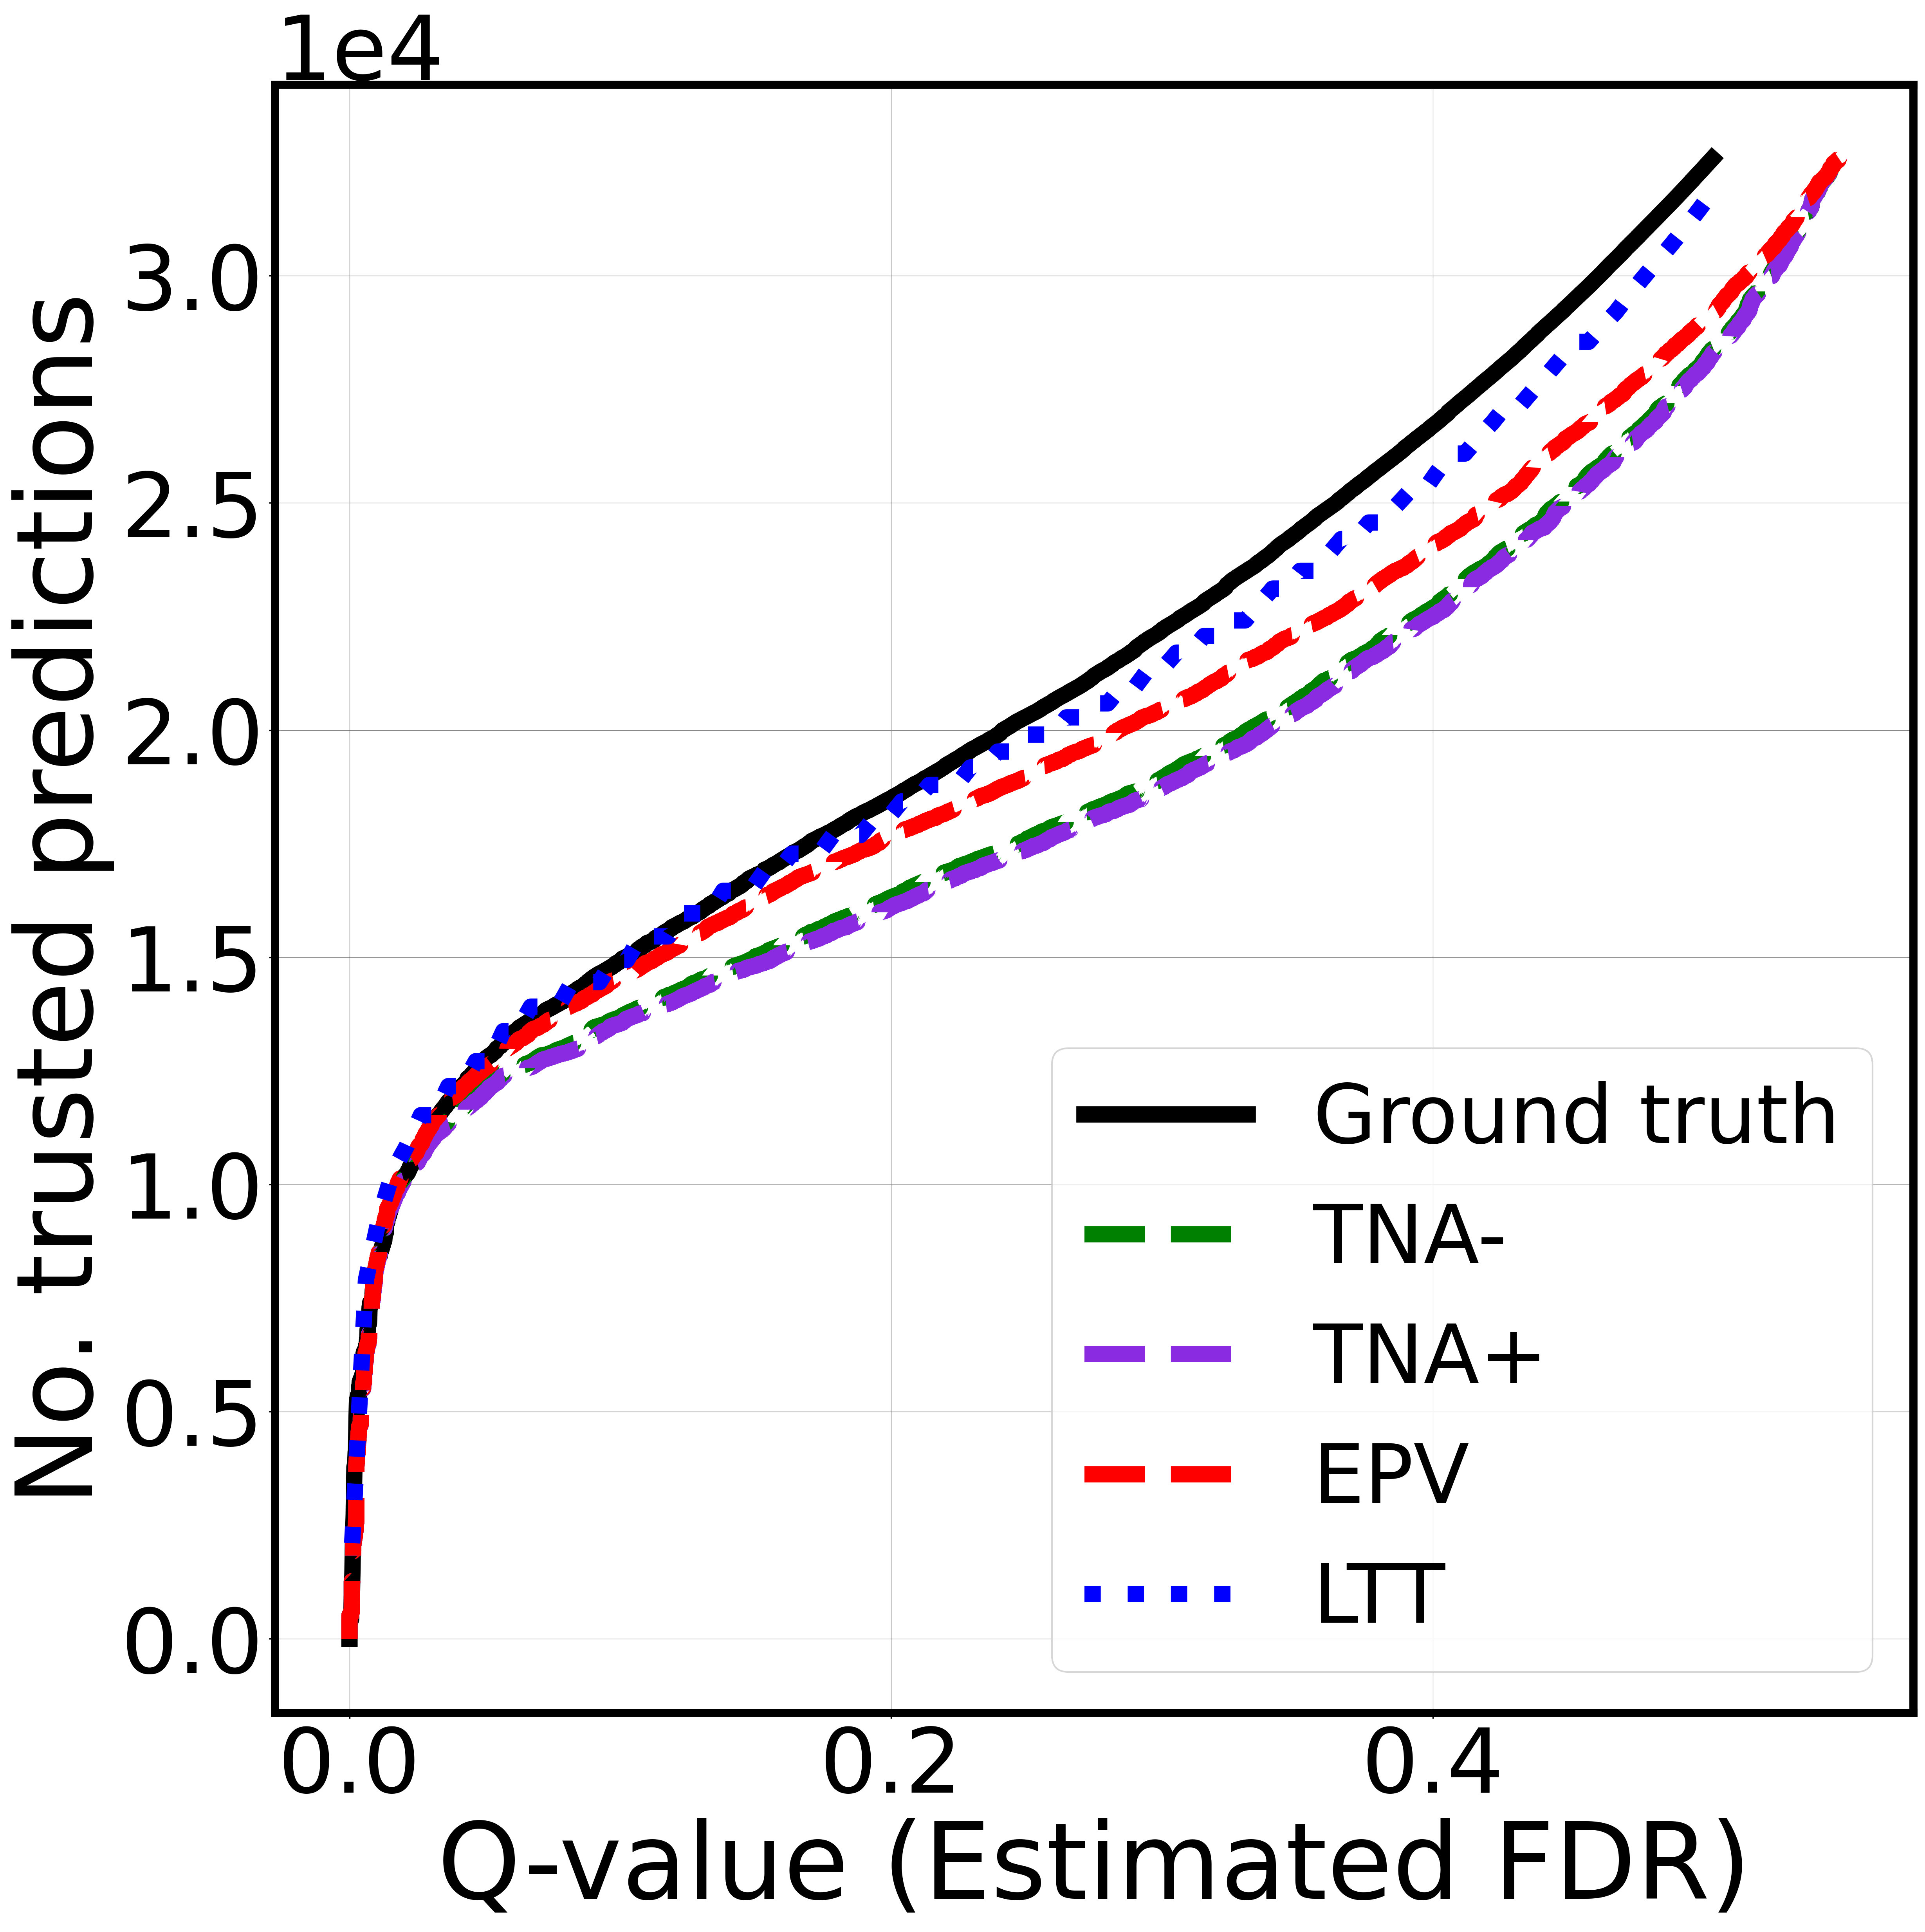
\includegraphics[width=0.225\linewidth, height=0.225\linewidth]{img/cnn_pcam_fdr_control.png} & 
		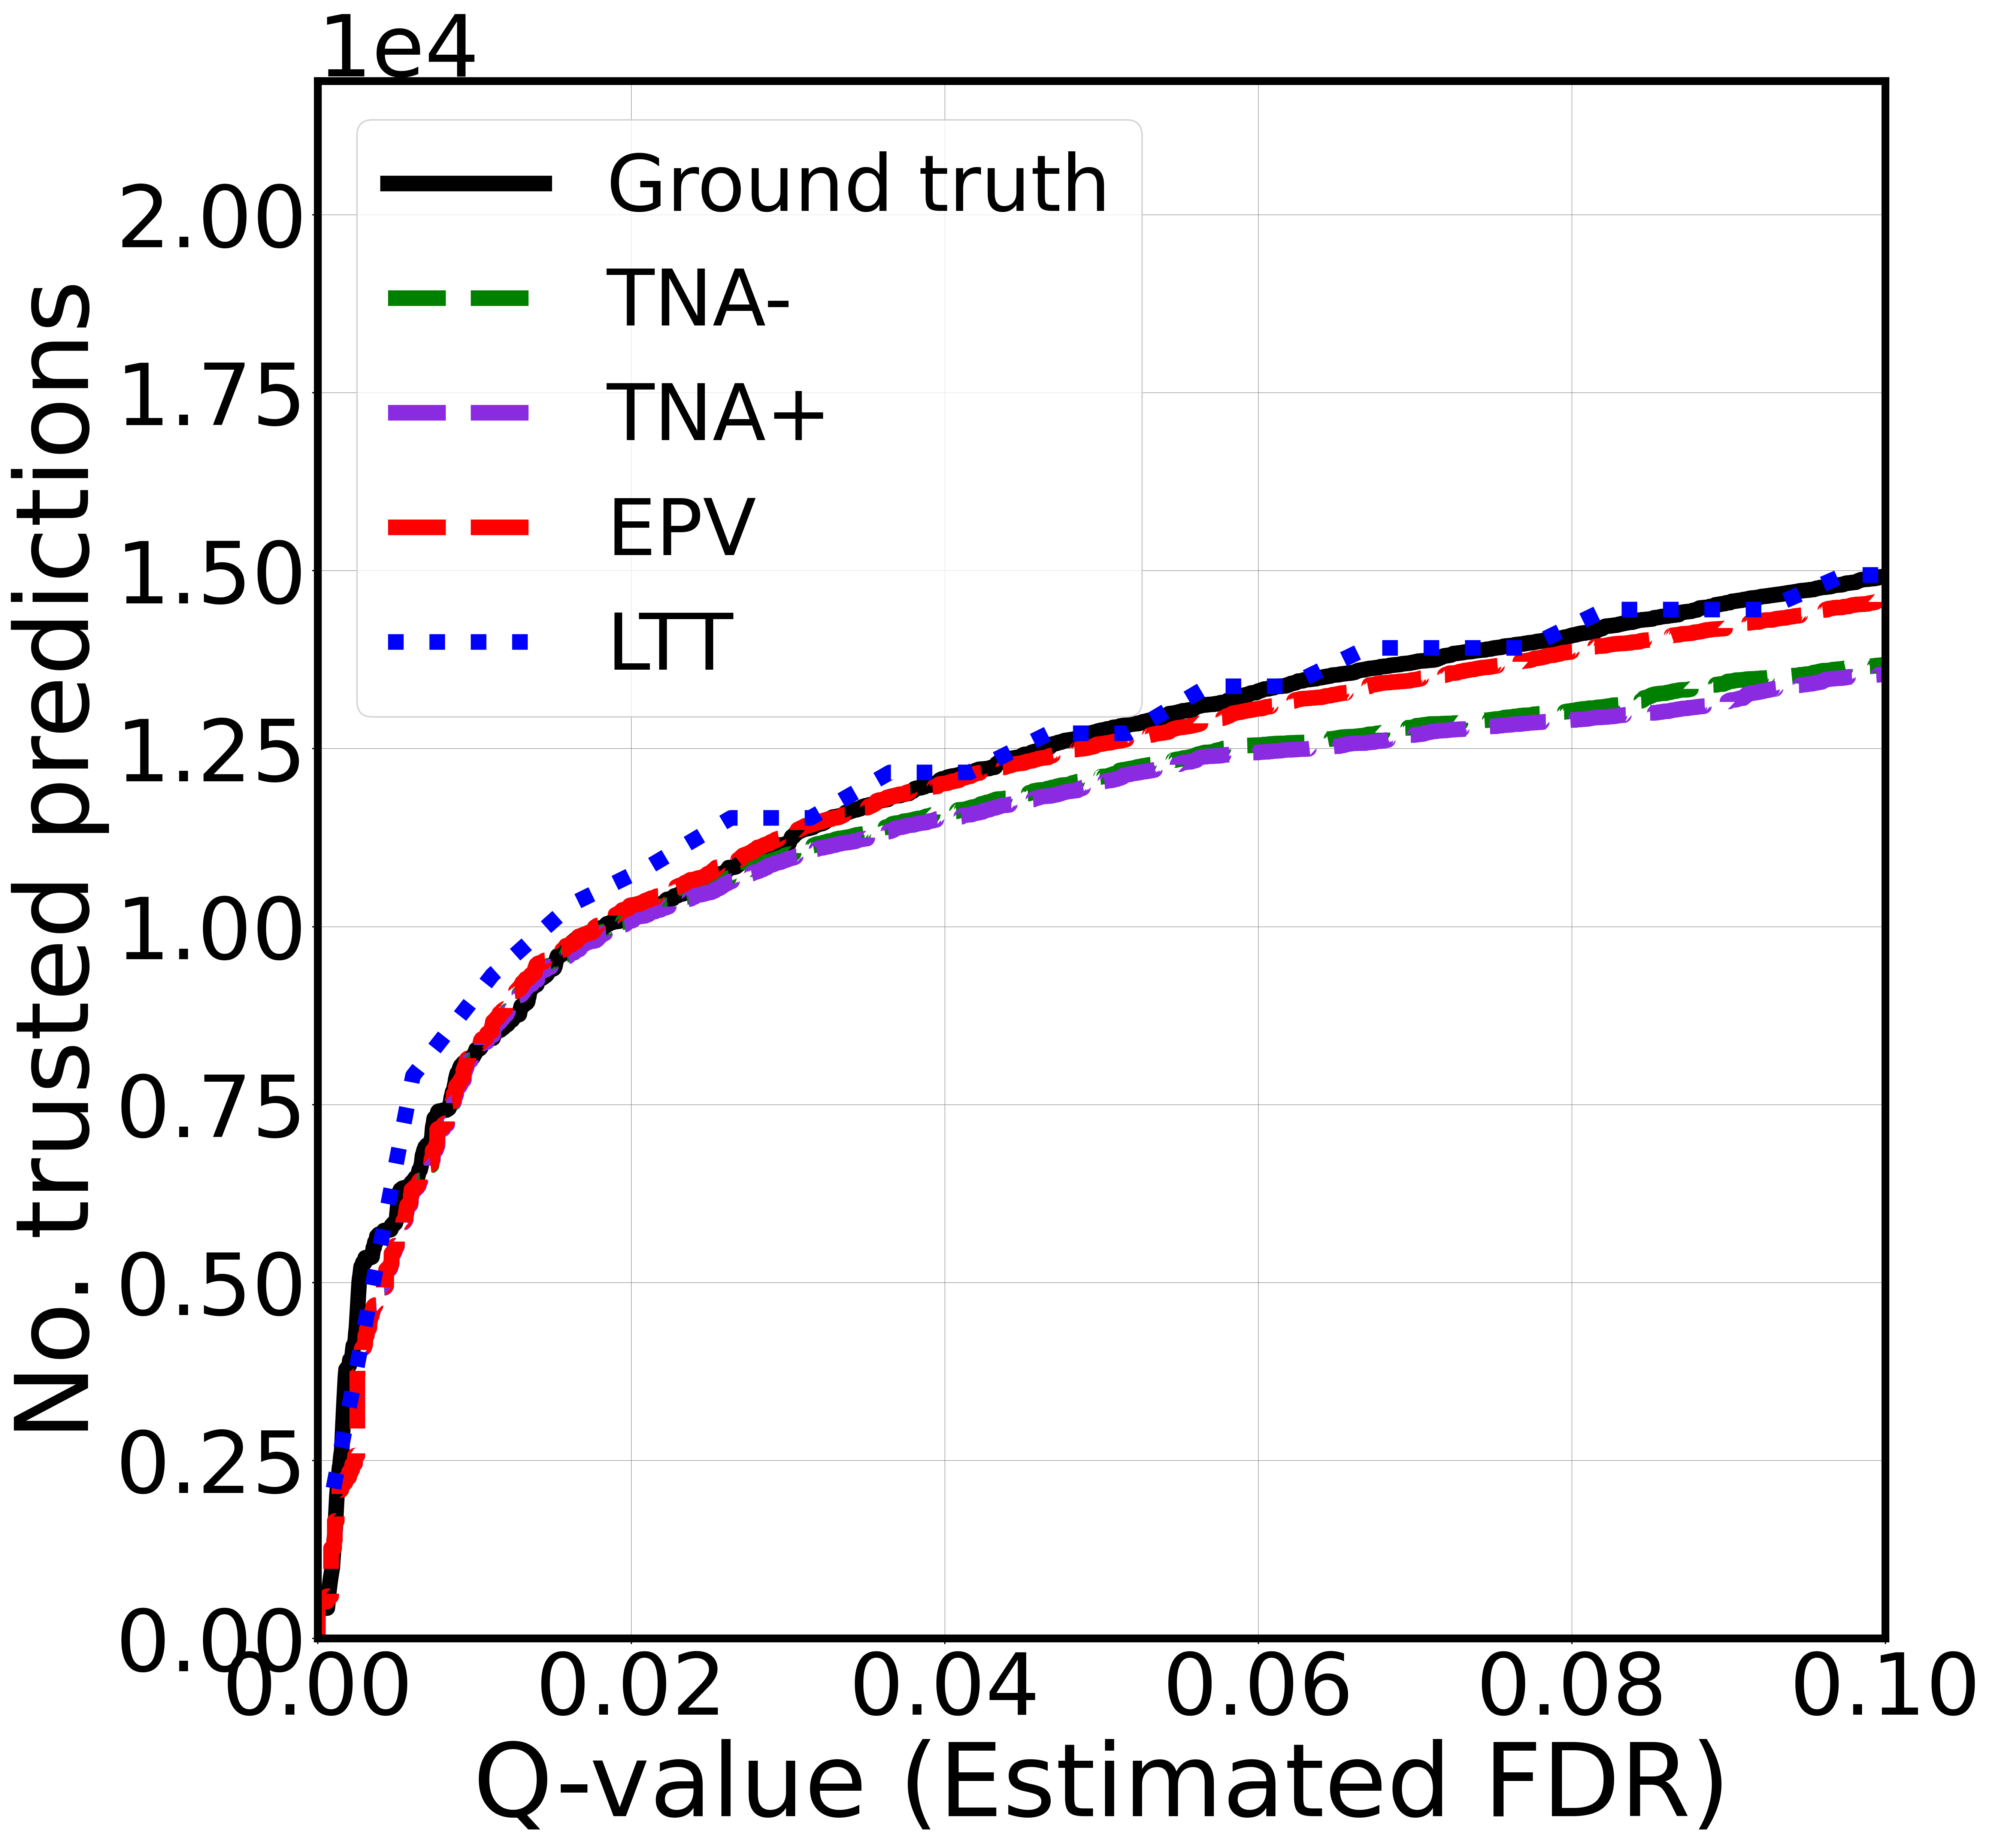
\includegraphics[width=0.225\linewidth, height=0.225\linewidth]{img/cnn_pcam_fdr_control_loc.png} &
		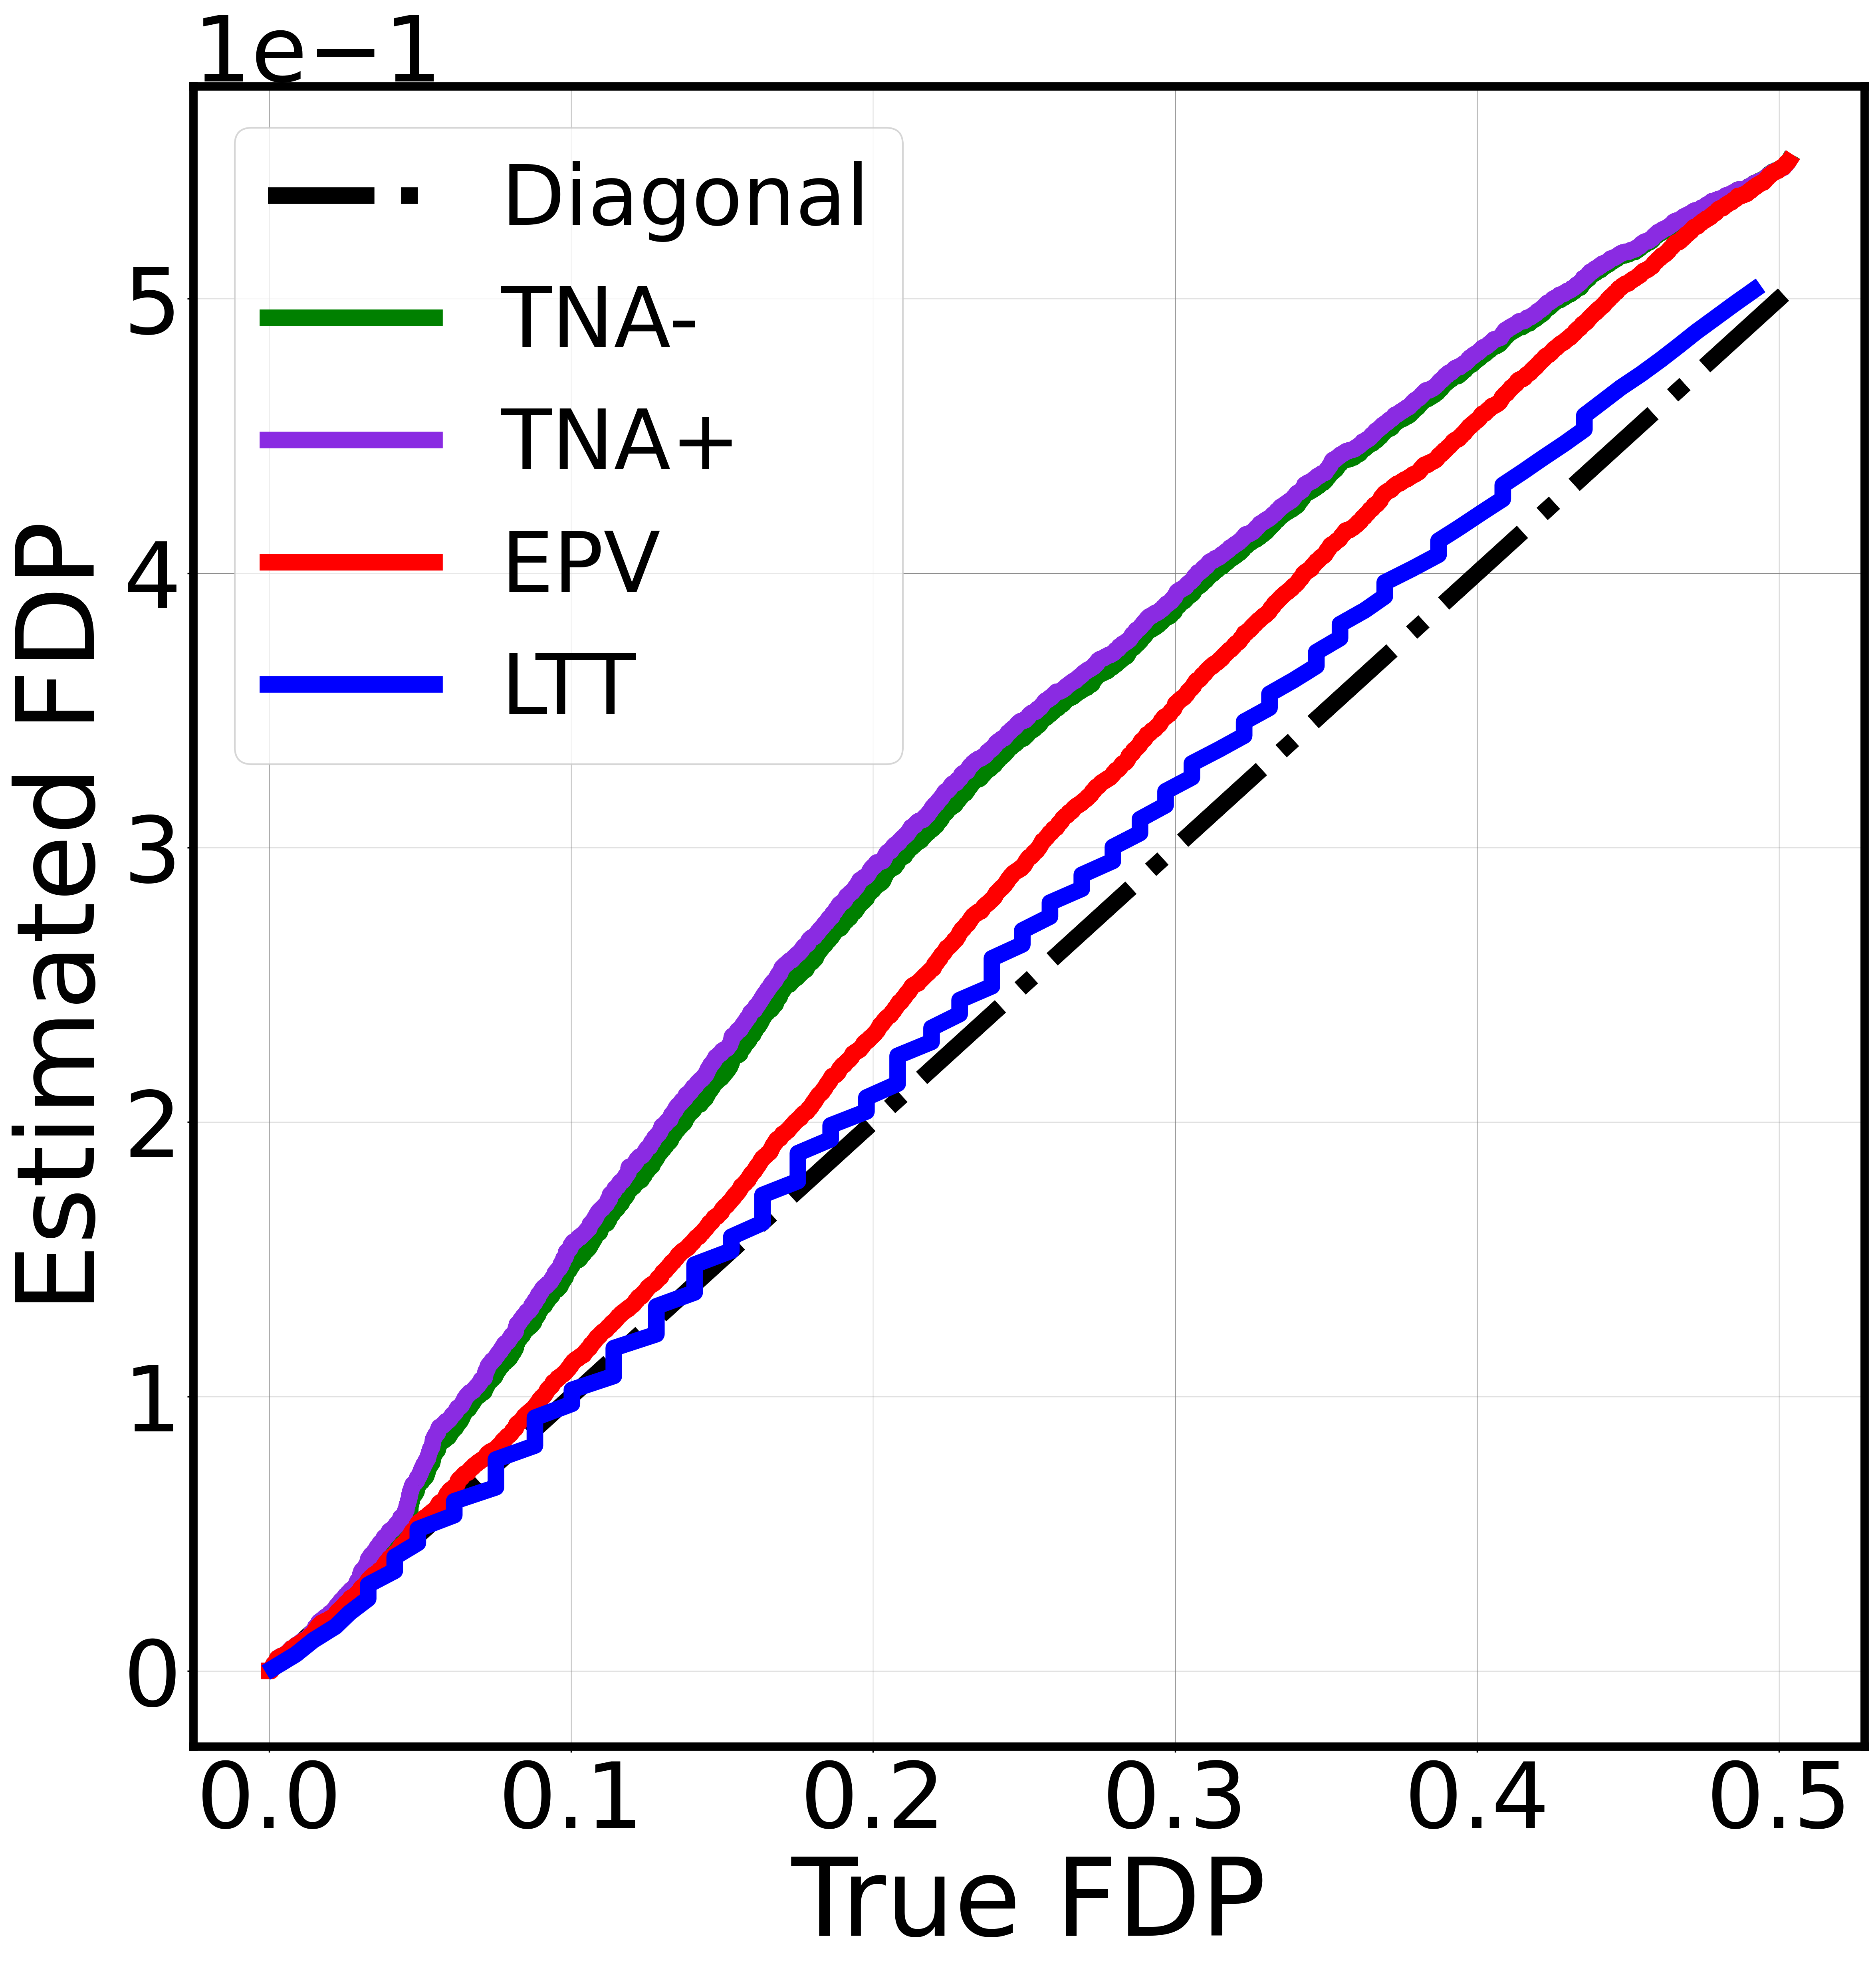
\includegraphics[width=0.225\linewidth, height=0.225\linewidth]{img/cnn_FDPscat_pcam.png}\\	
		\multicolumn{4}{l}{\bf (ii) PCam with class distribution shift:}\\		
		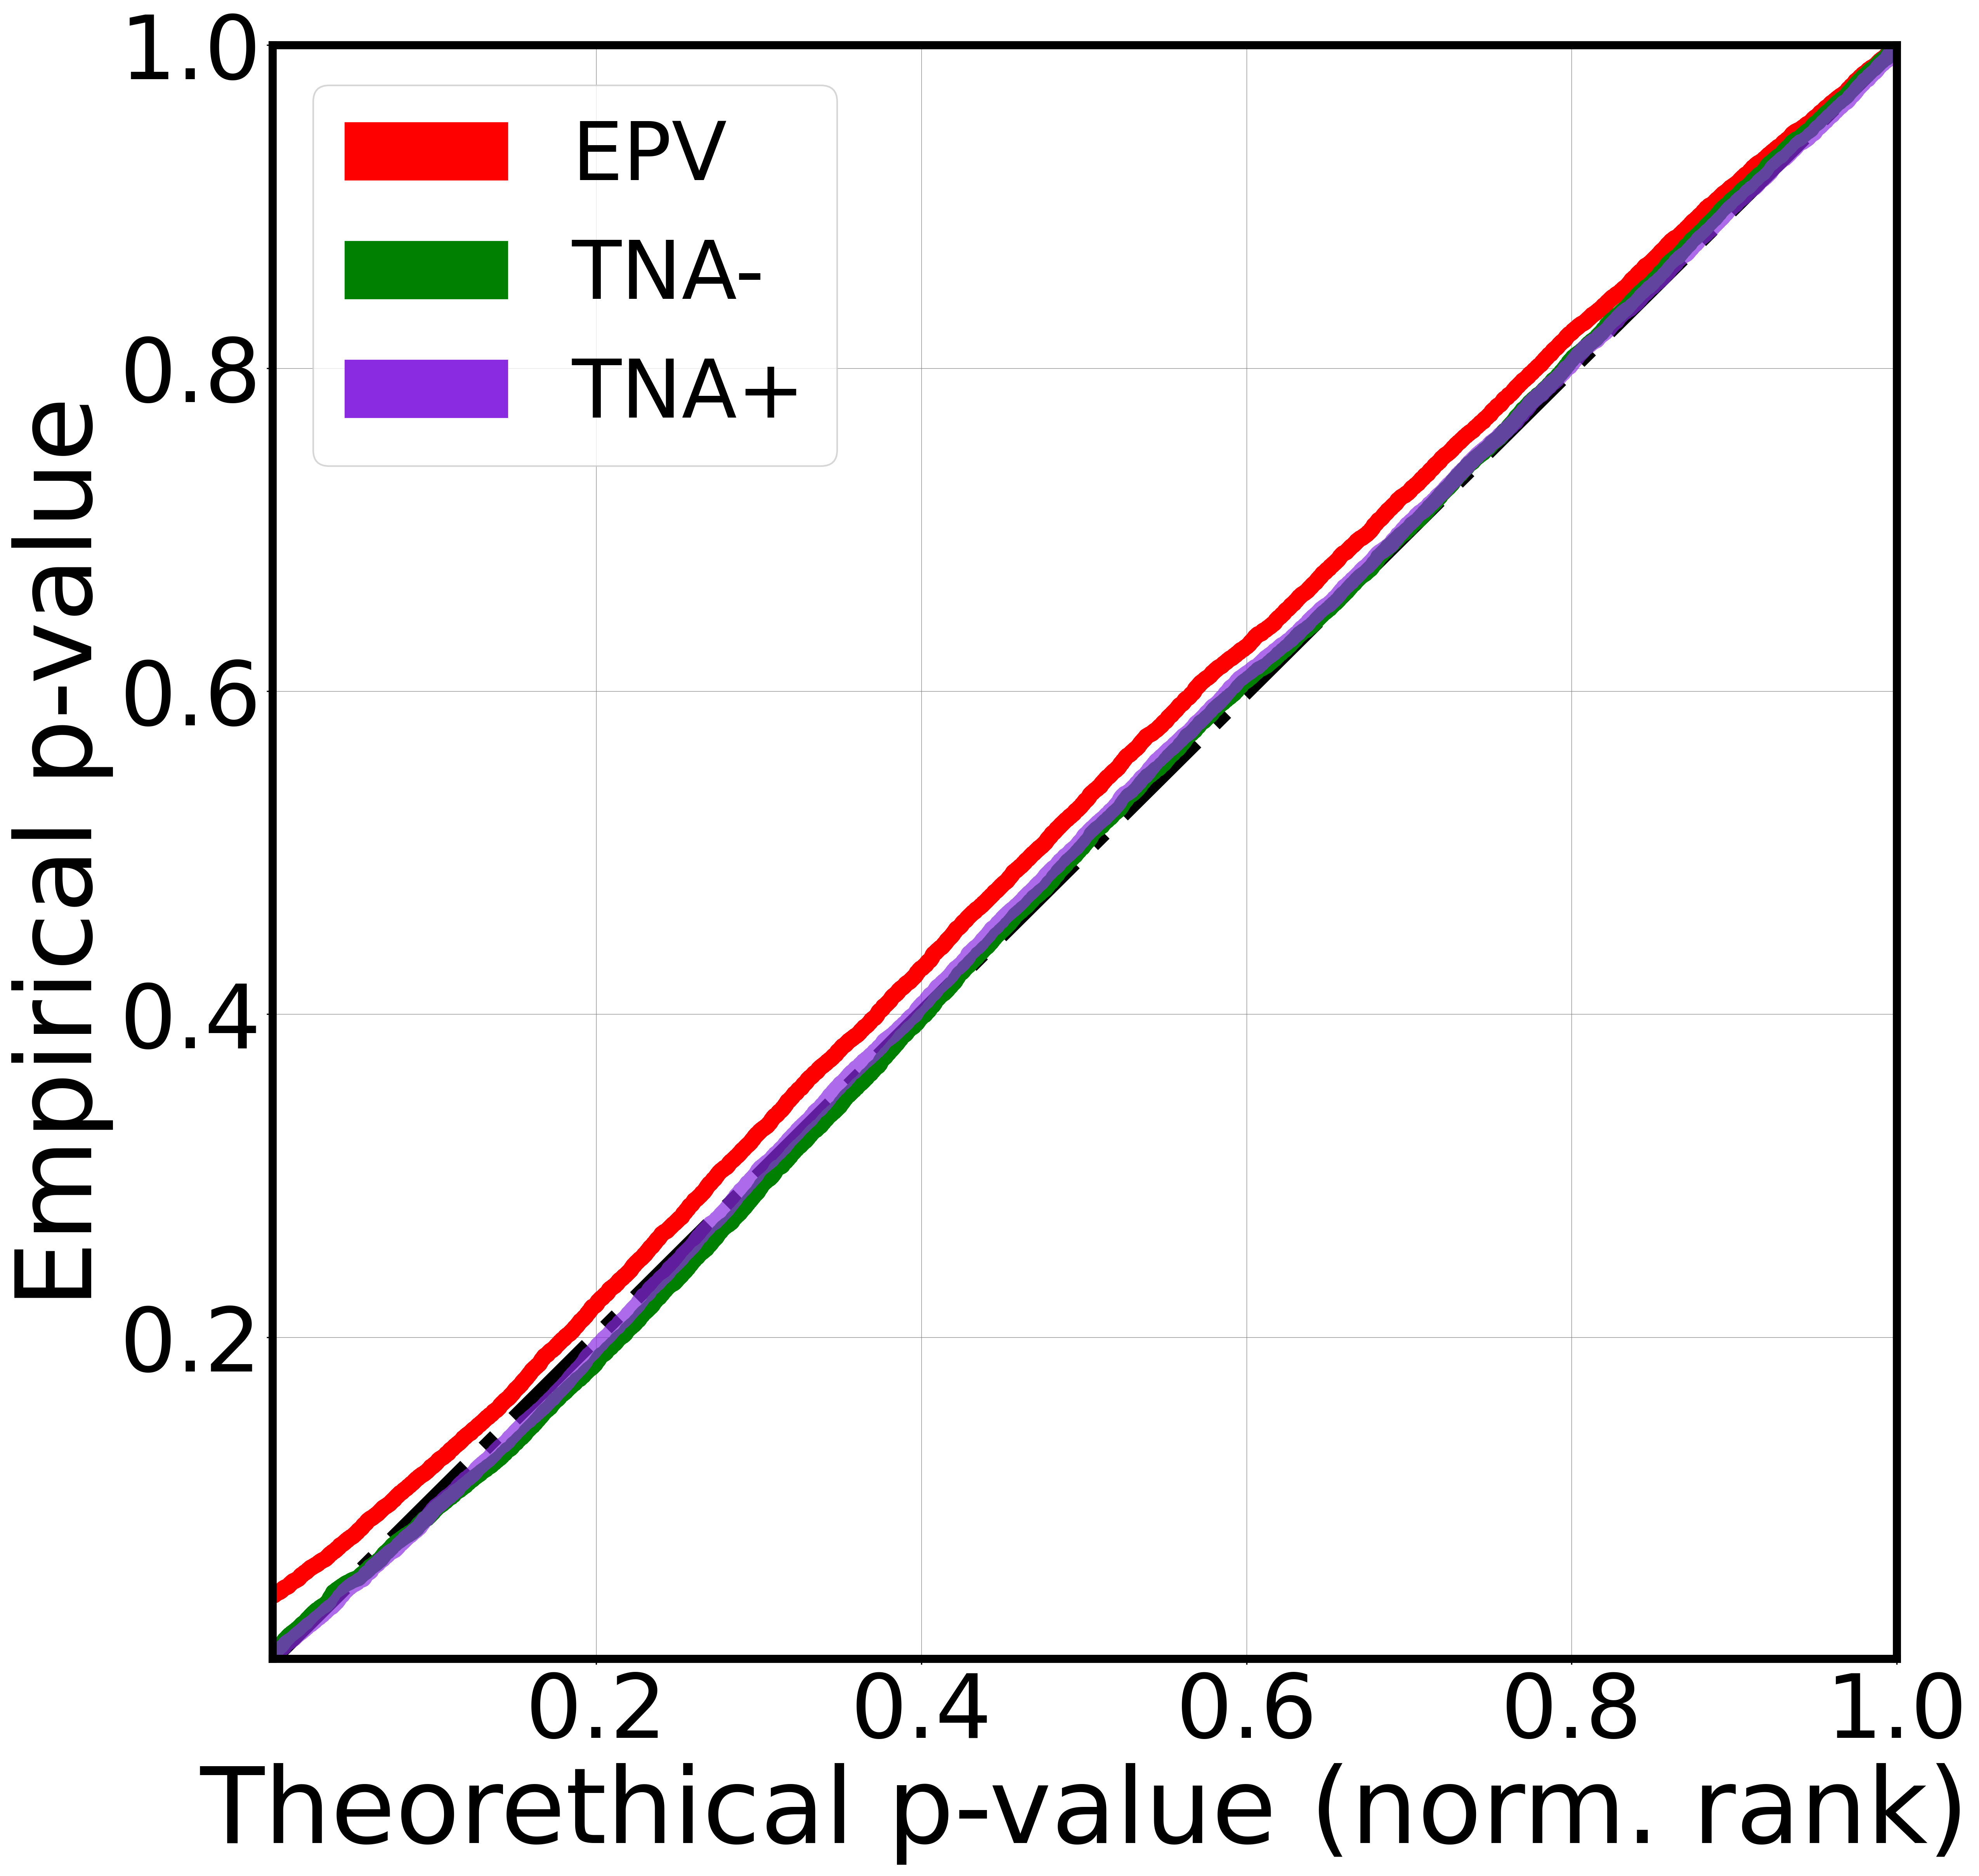
\includegraphics[width=0.225\linewidth, height=0.225\linewidth]{img/cnn_QQ_pcam_balanced.png} &
		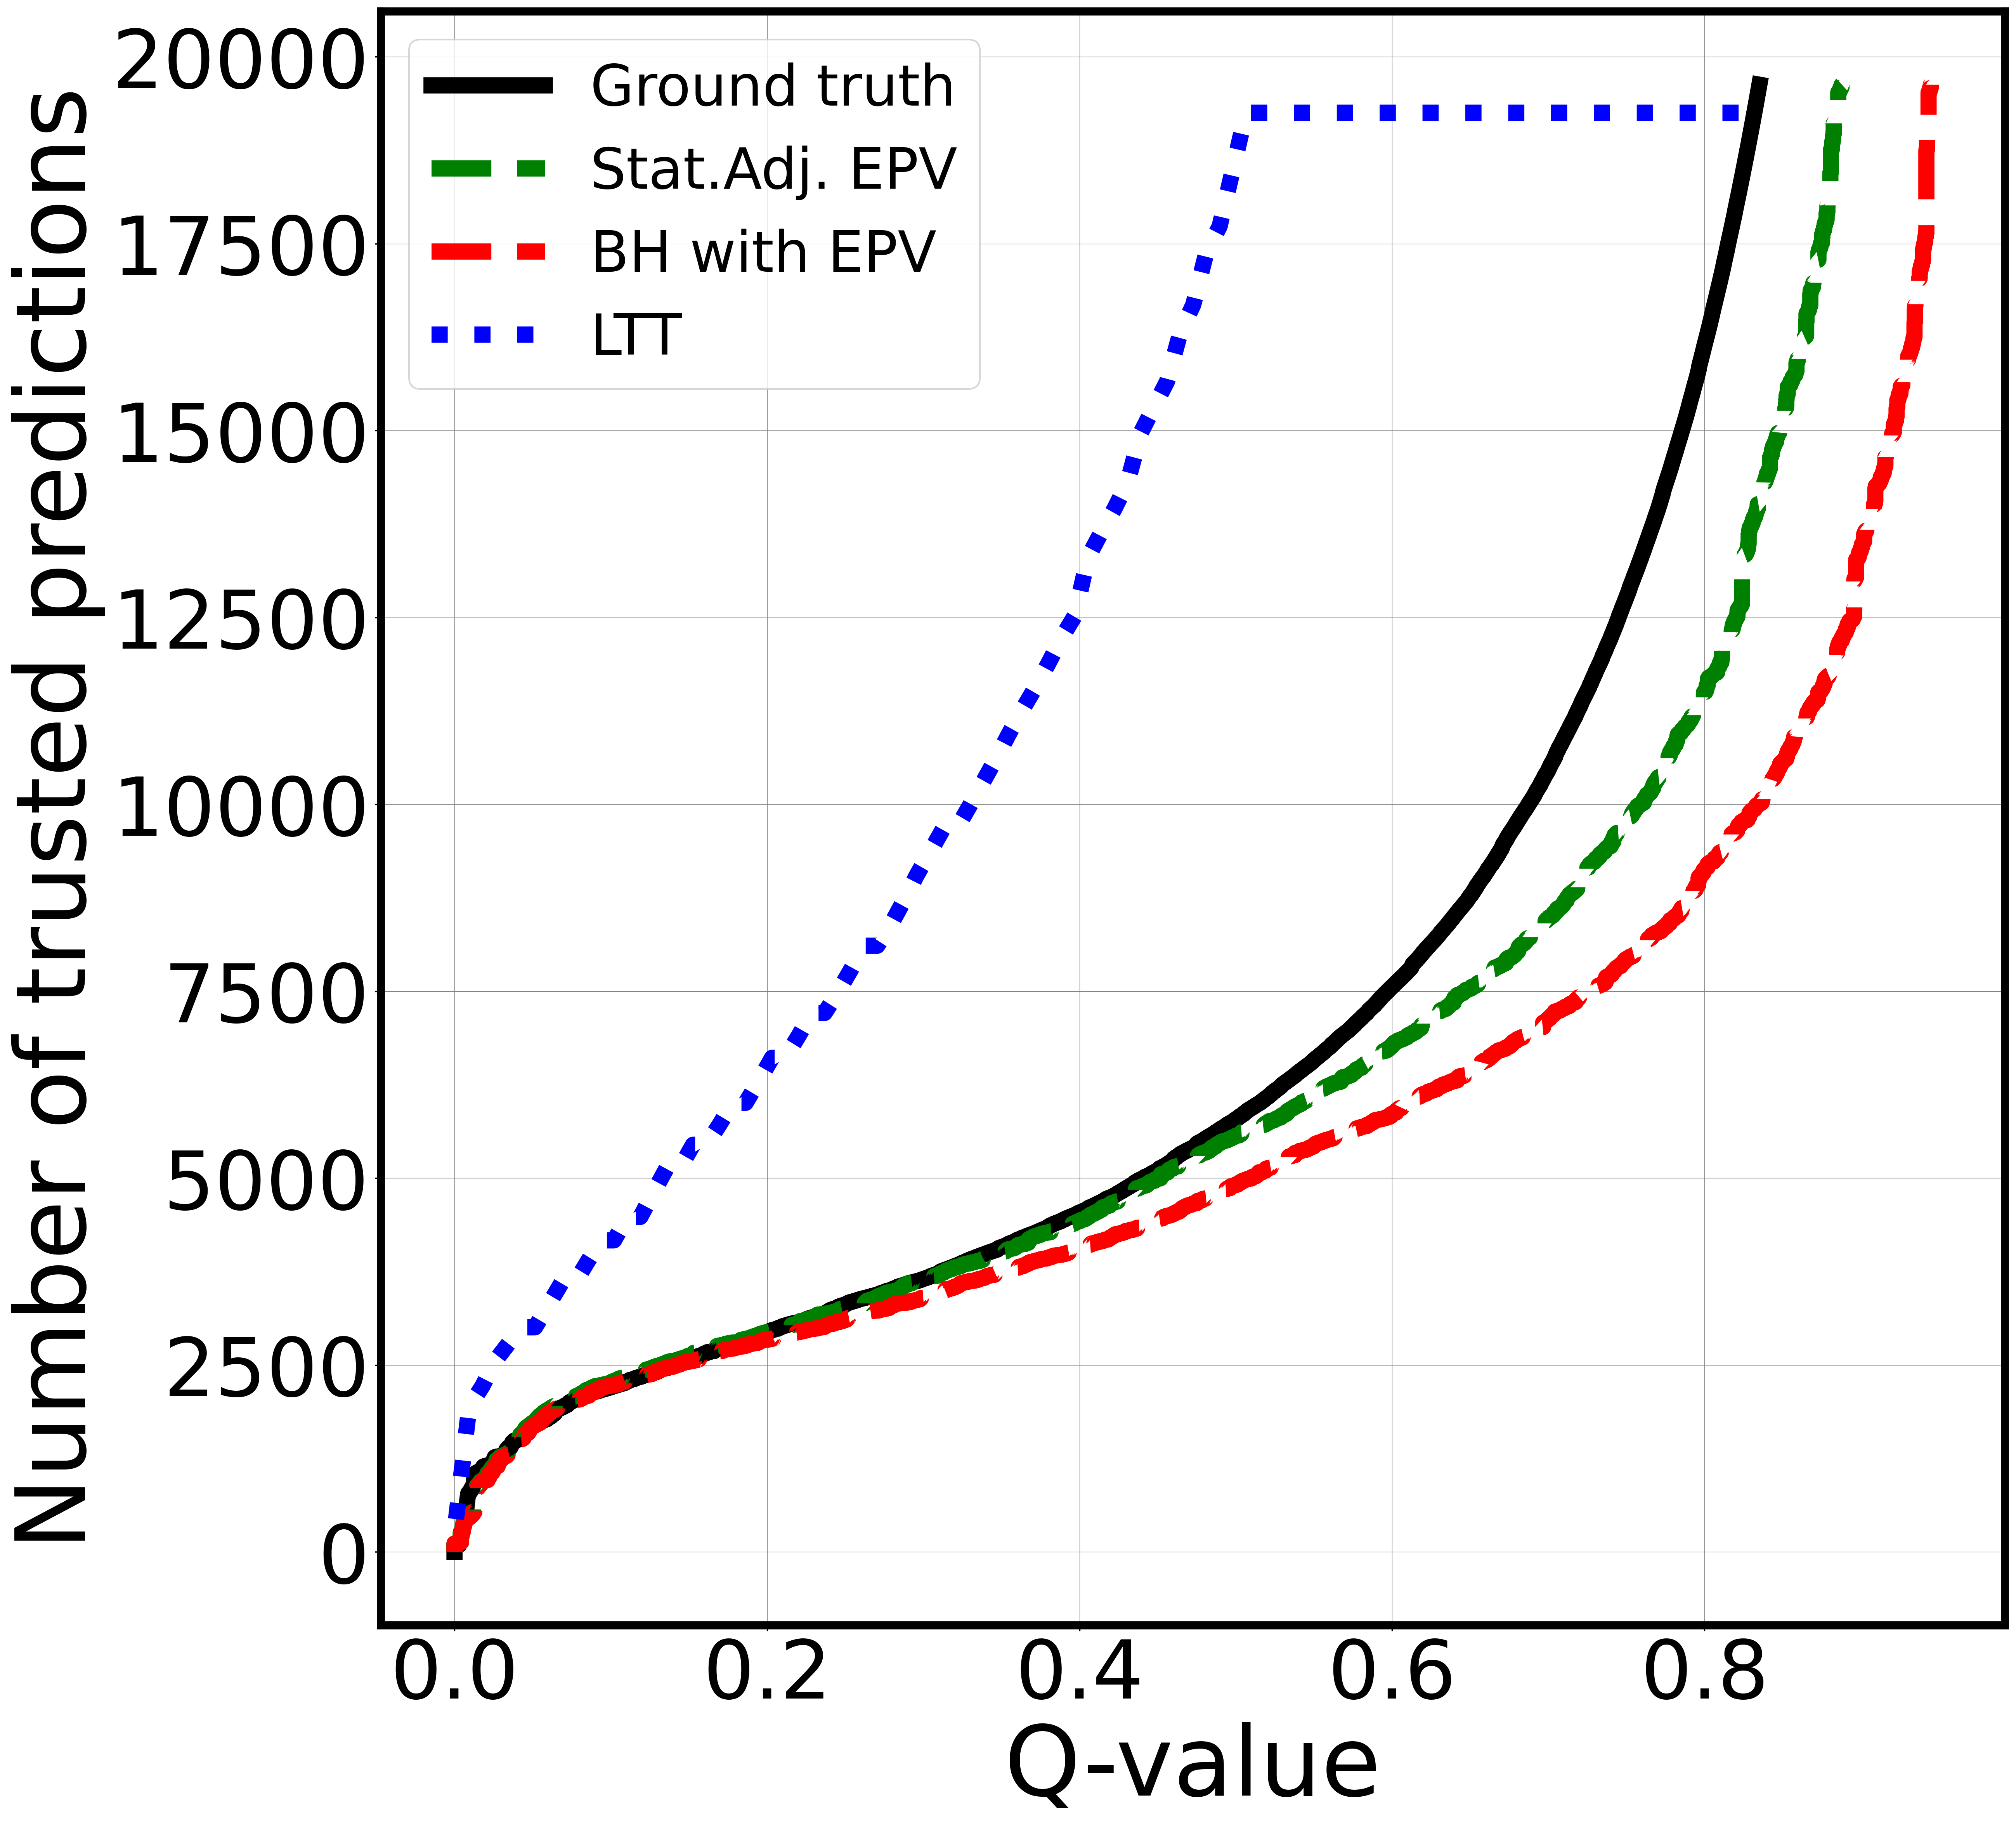
\includegraphics[width=0.225\linewidth, height=0.225\linewidth]{img/cnn_pcam_balanced_fdr_control.png} & 
		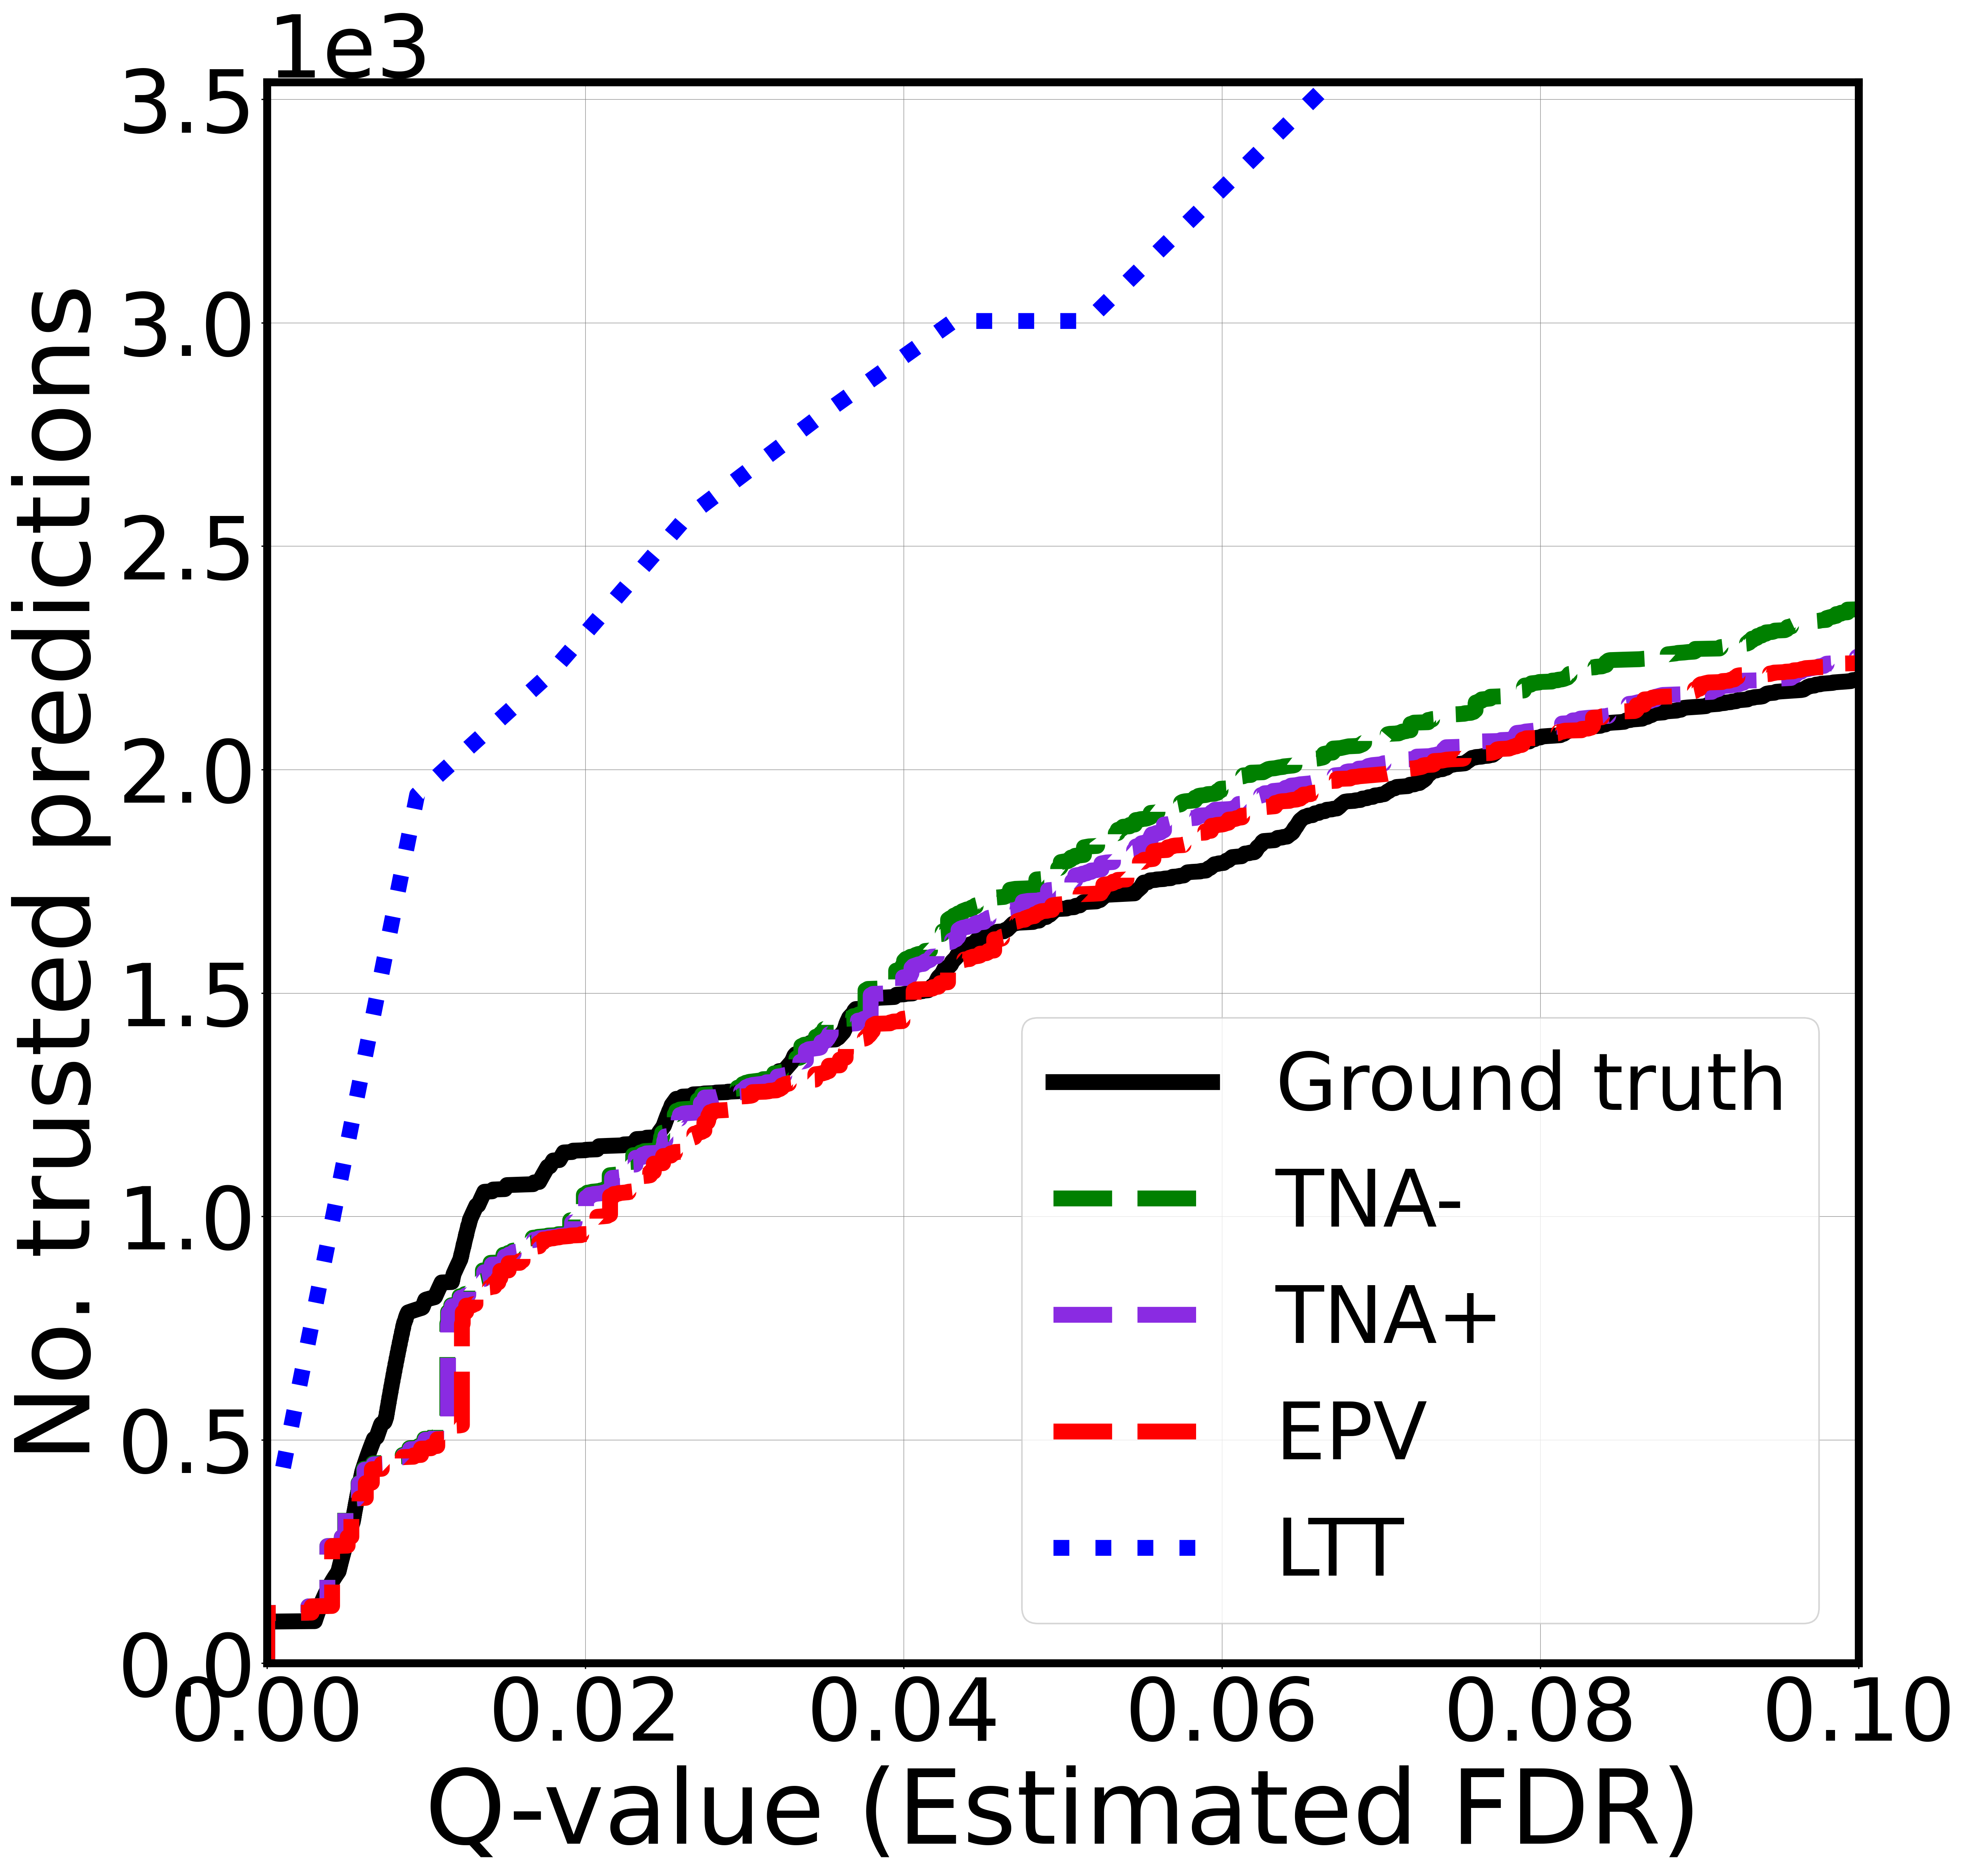
\includegraphics[width=0.225\linewidth, height=0.225\linewidth]{img/cnn_pcam_balanced_fdr_control_loc.png} &
		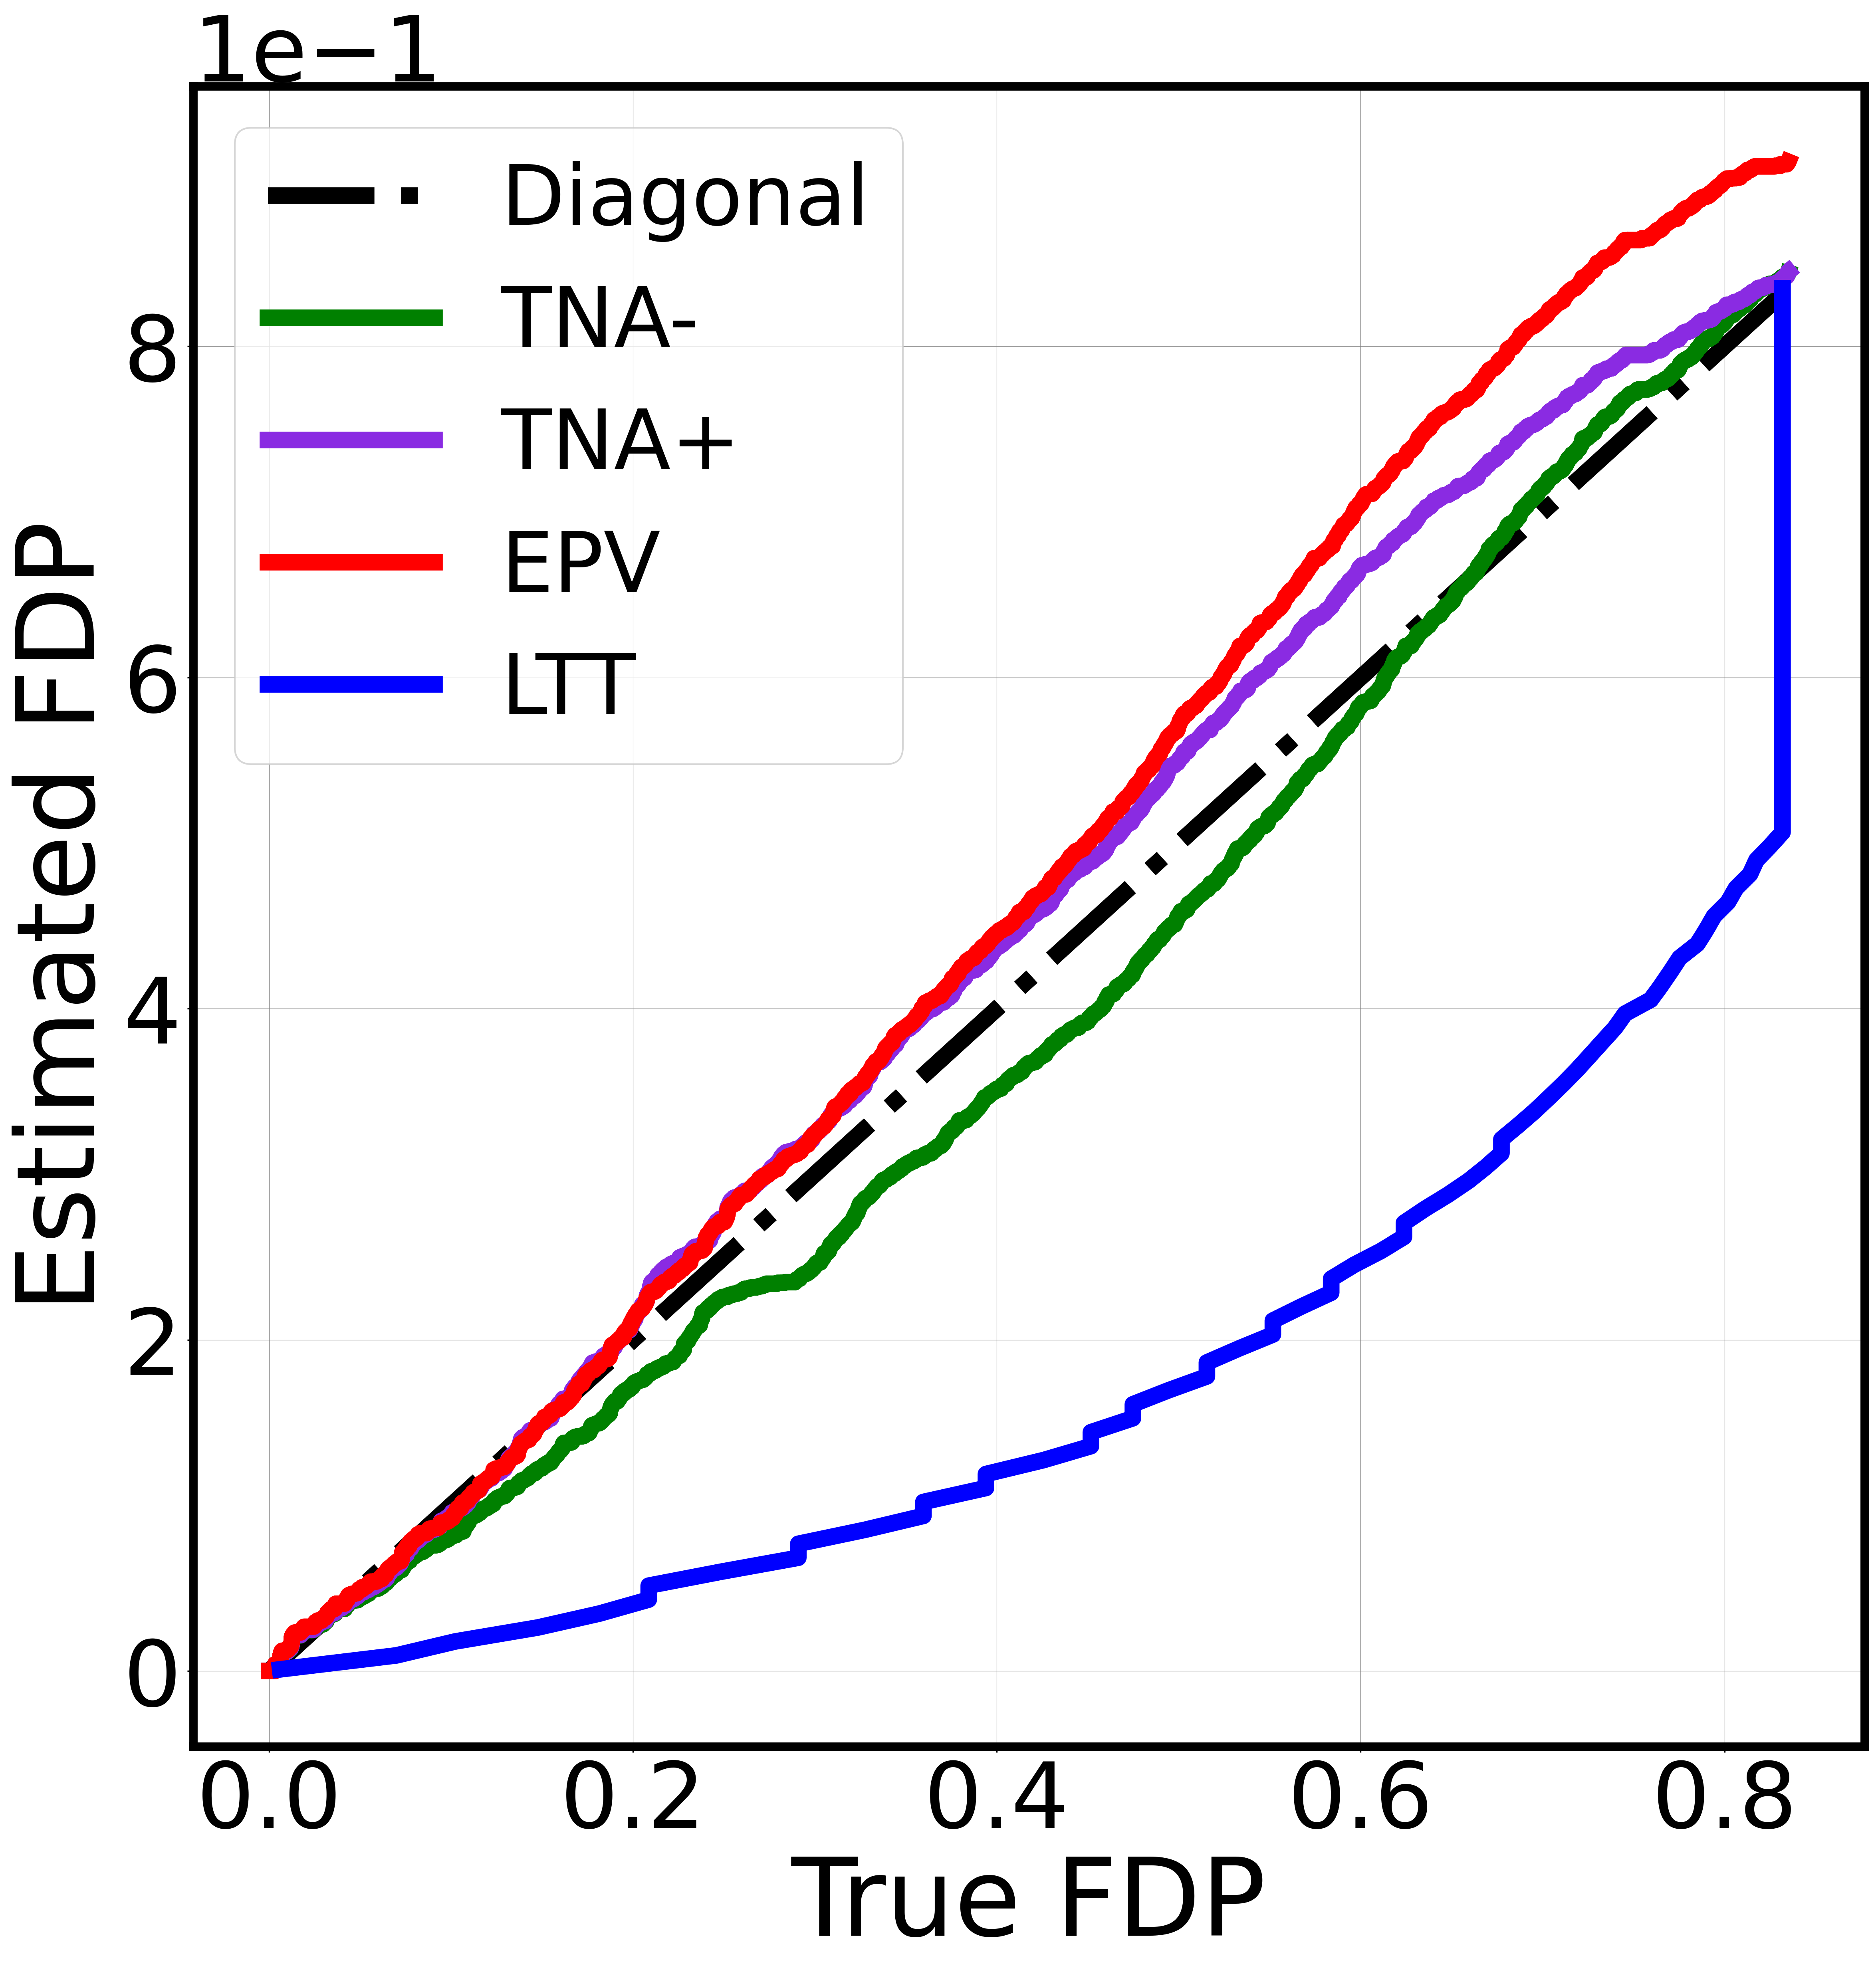
\includegraphics[width=0.225\linewidth, height=0.225\linewidth]{img/cnn_FDPscat_pcam_balanced.png}\\
		\multicolumn{4}{l}{\bf (iii) Standard CheXpert dataset:}\\	
		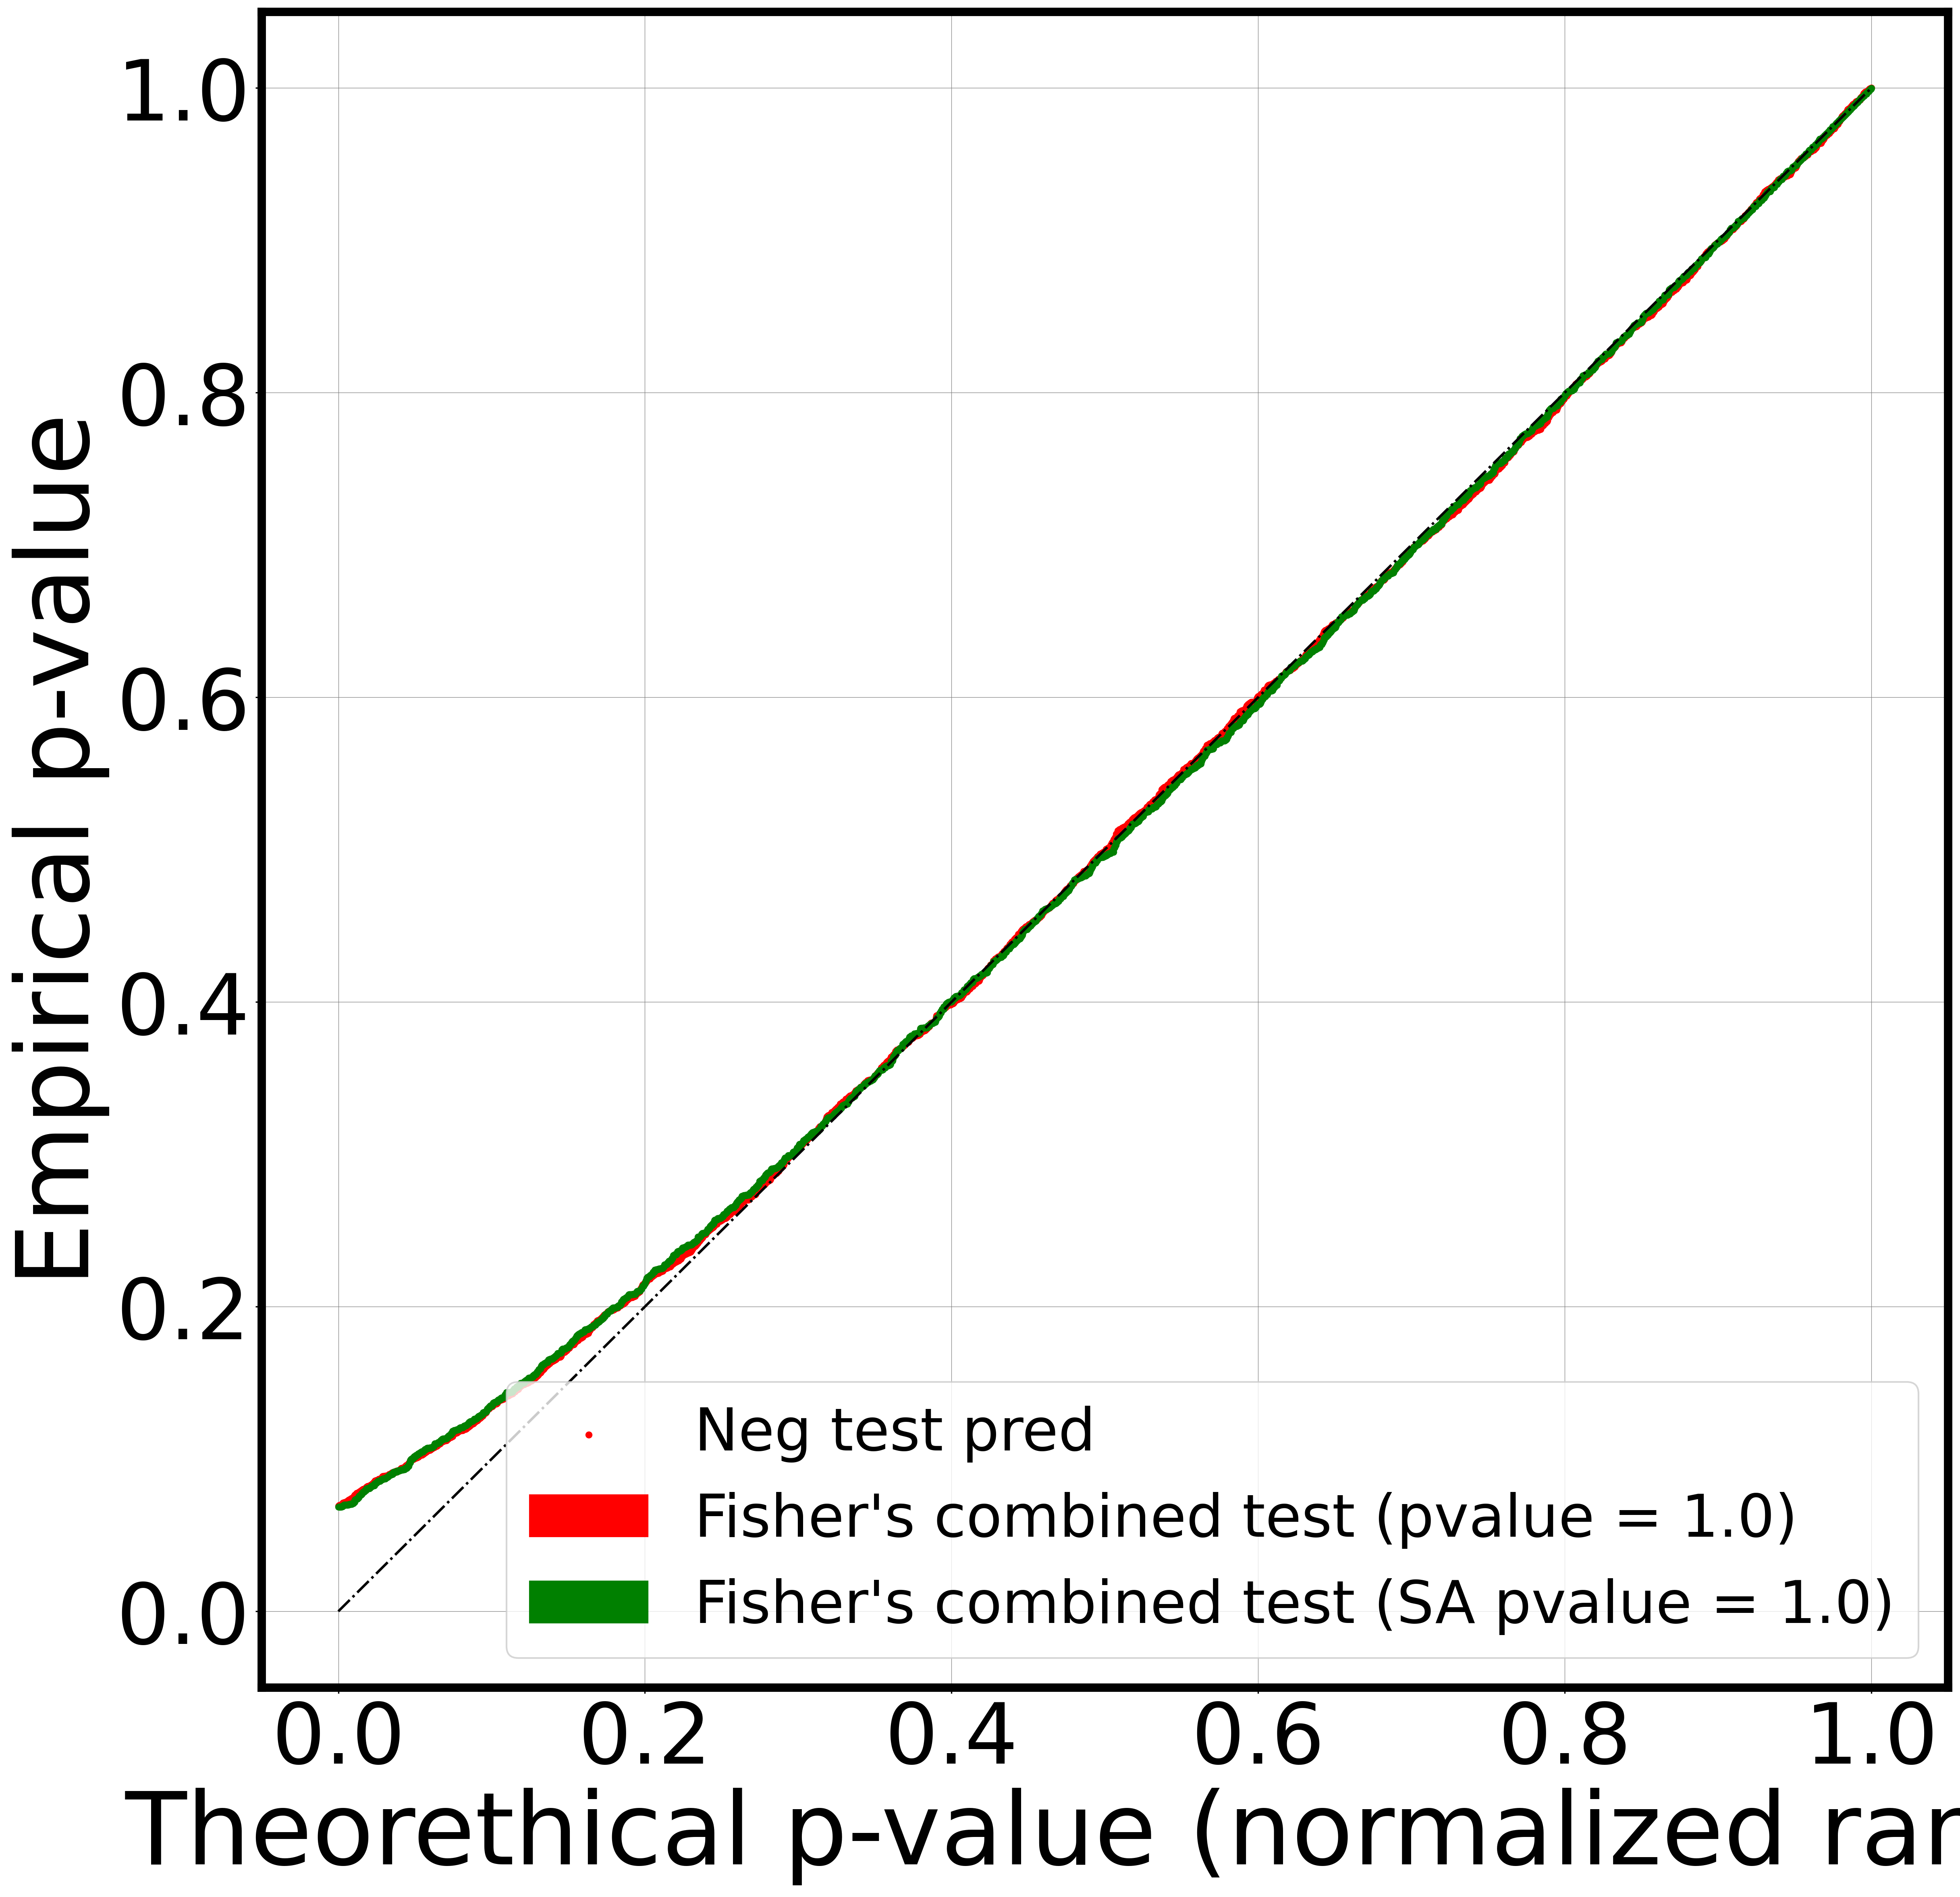
\includegraphics[width=0.225\linewidth, height=0.225\linewidth]{img/cnn_QQ_chx.png} 		&
		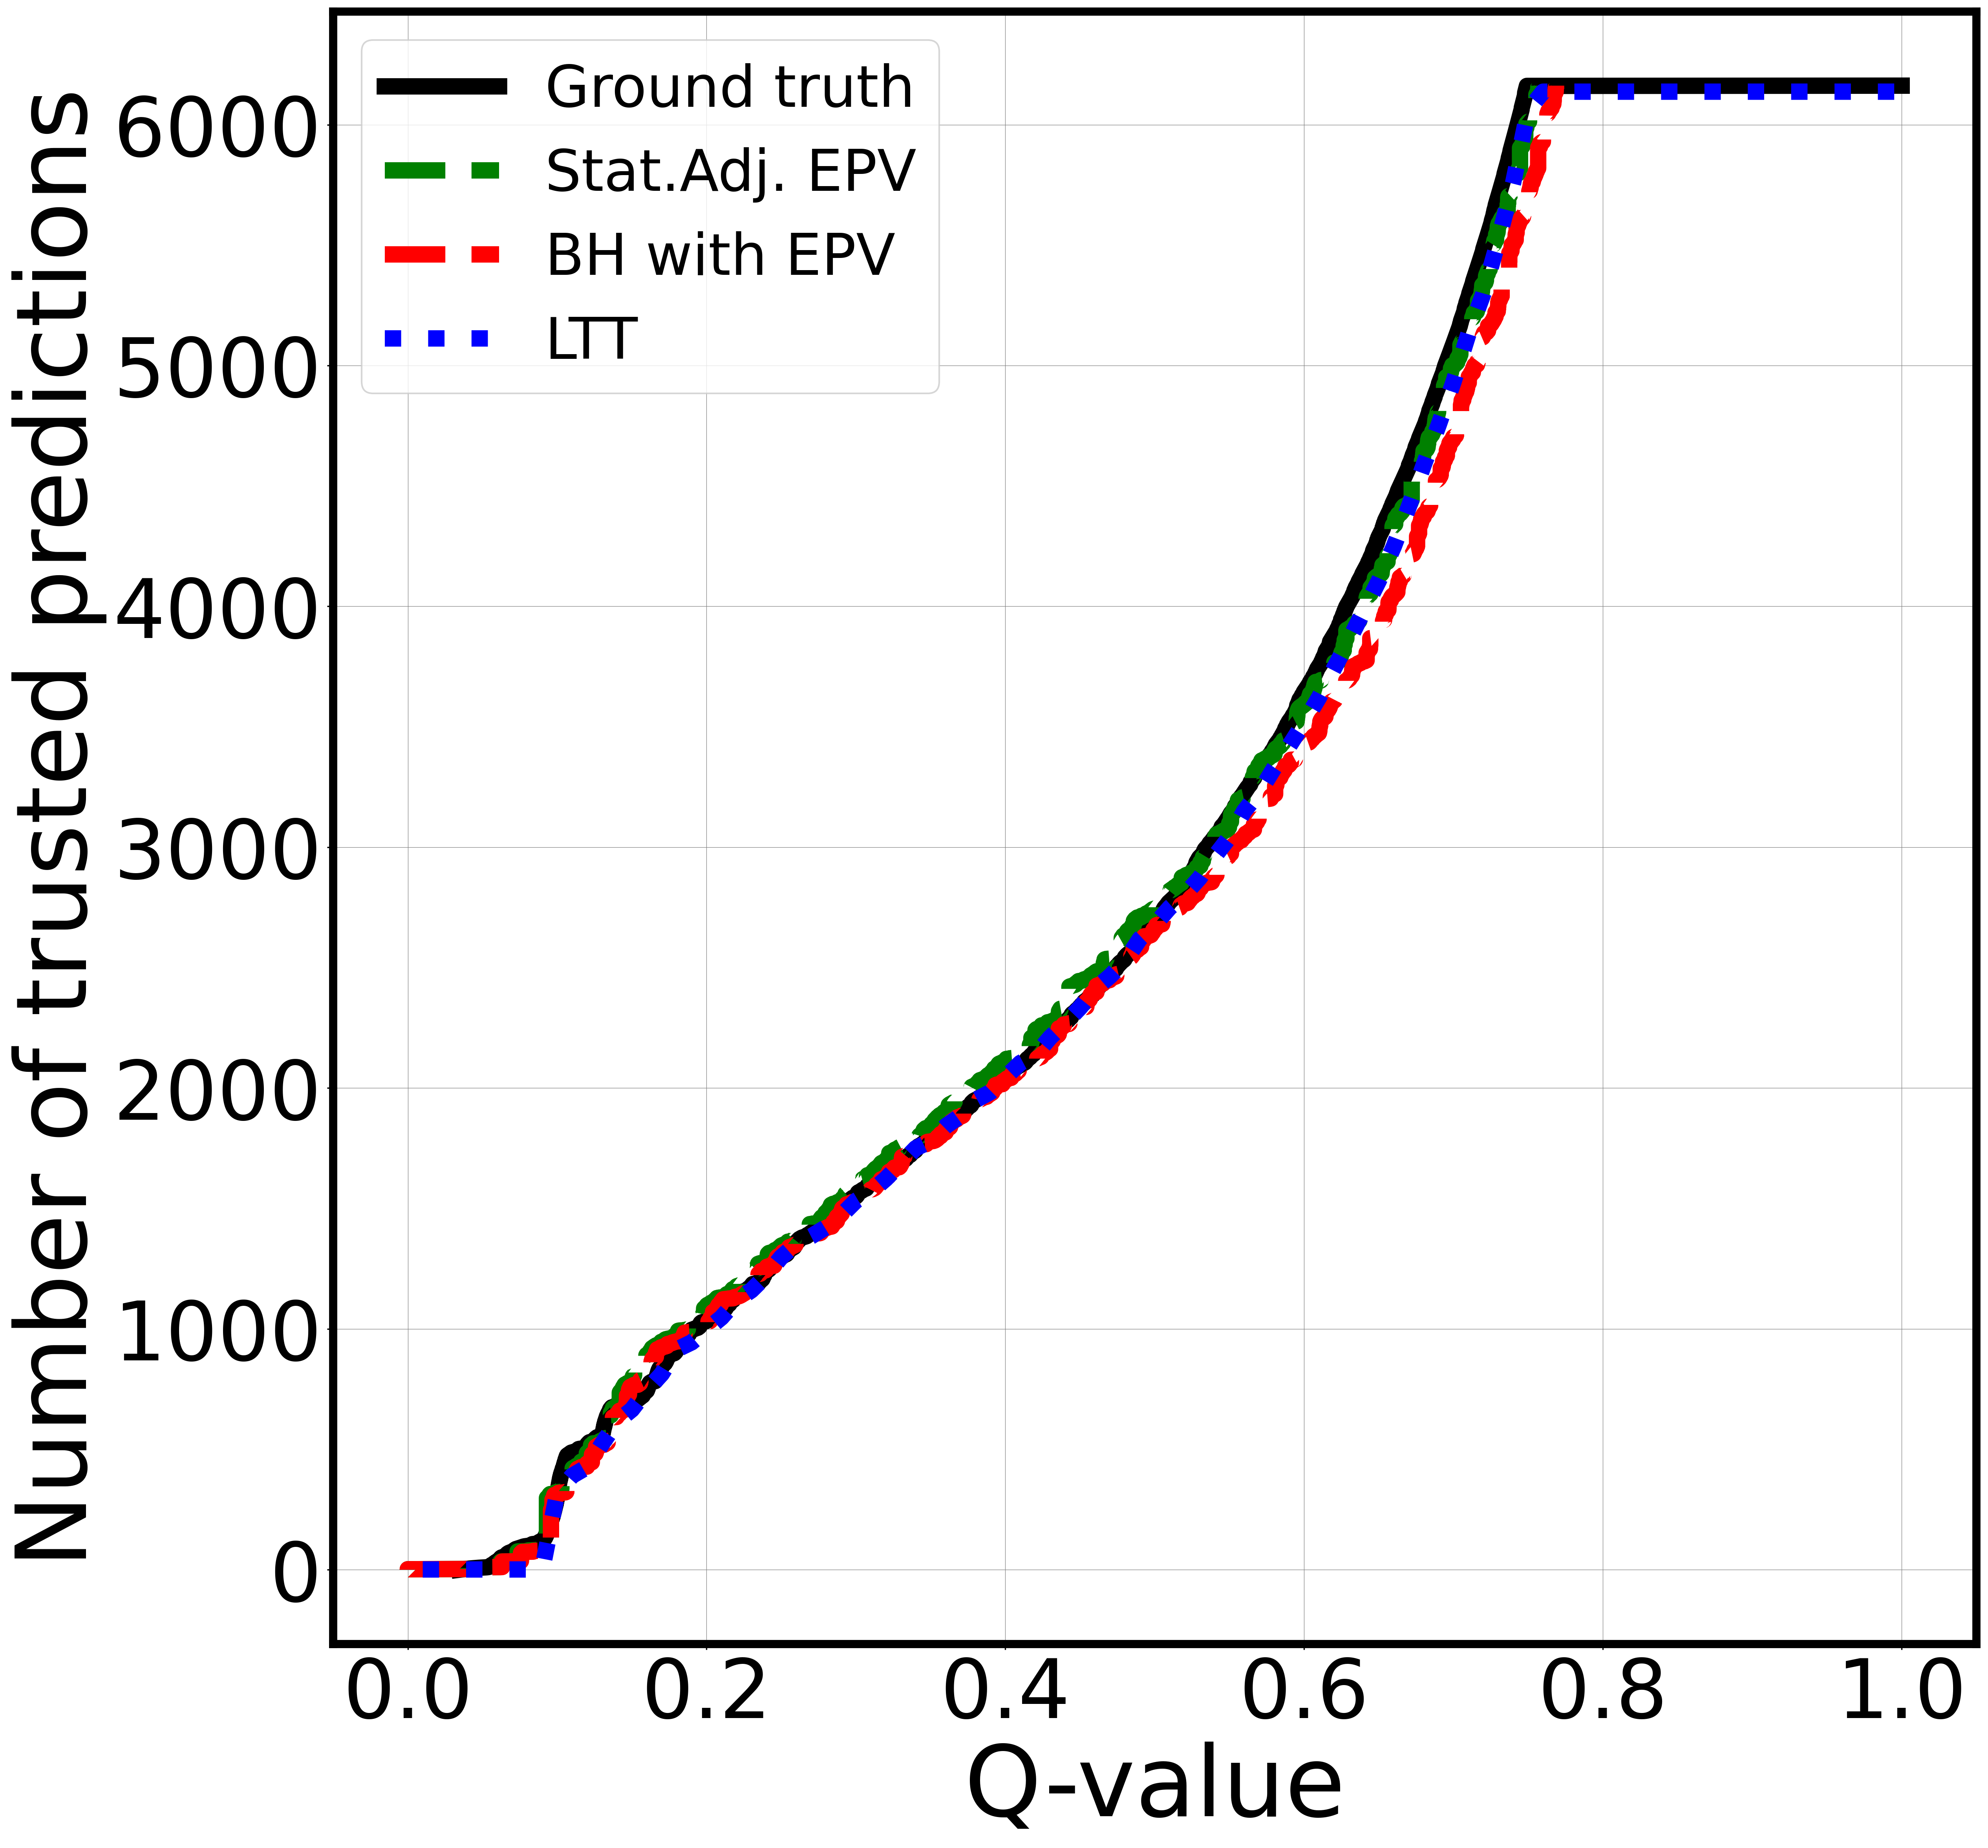
\includegraphics[width=0.225\linewidth, height=0.225\linewidth]{img/cnn_chx_fdr_control.png} & 
		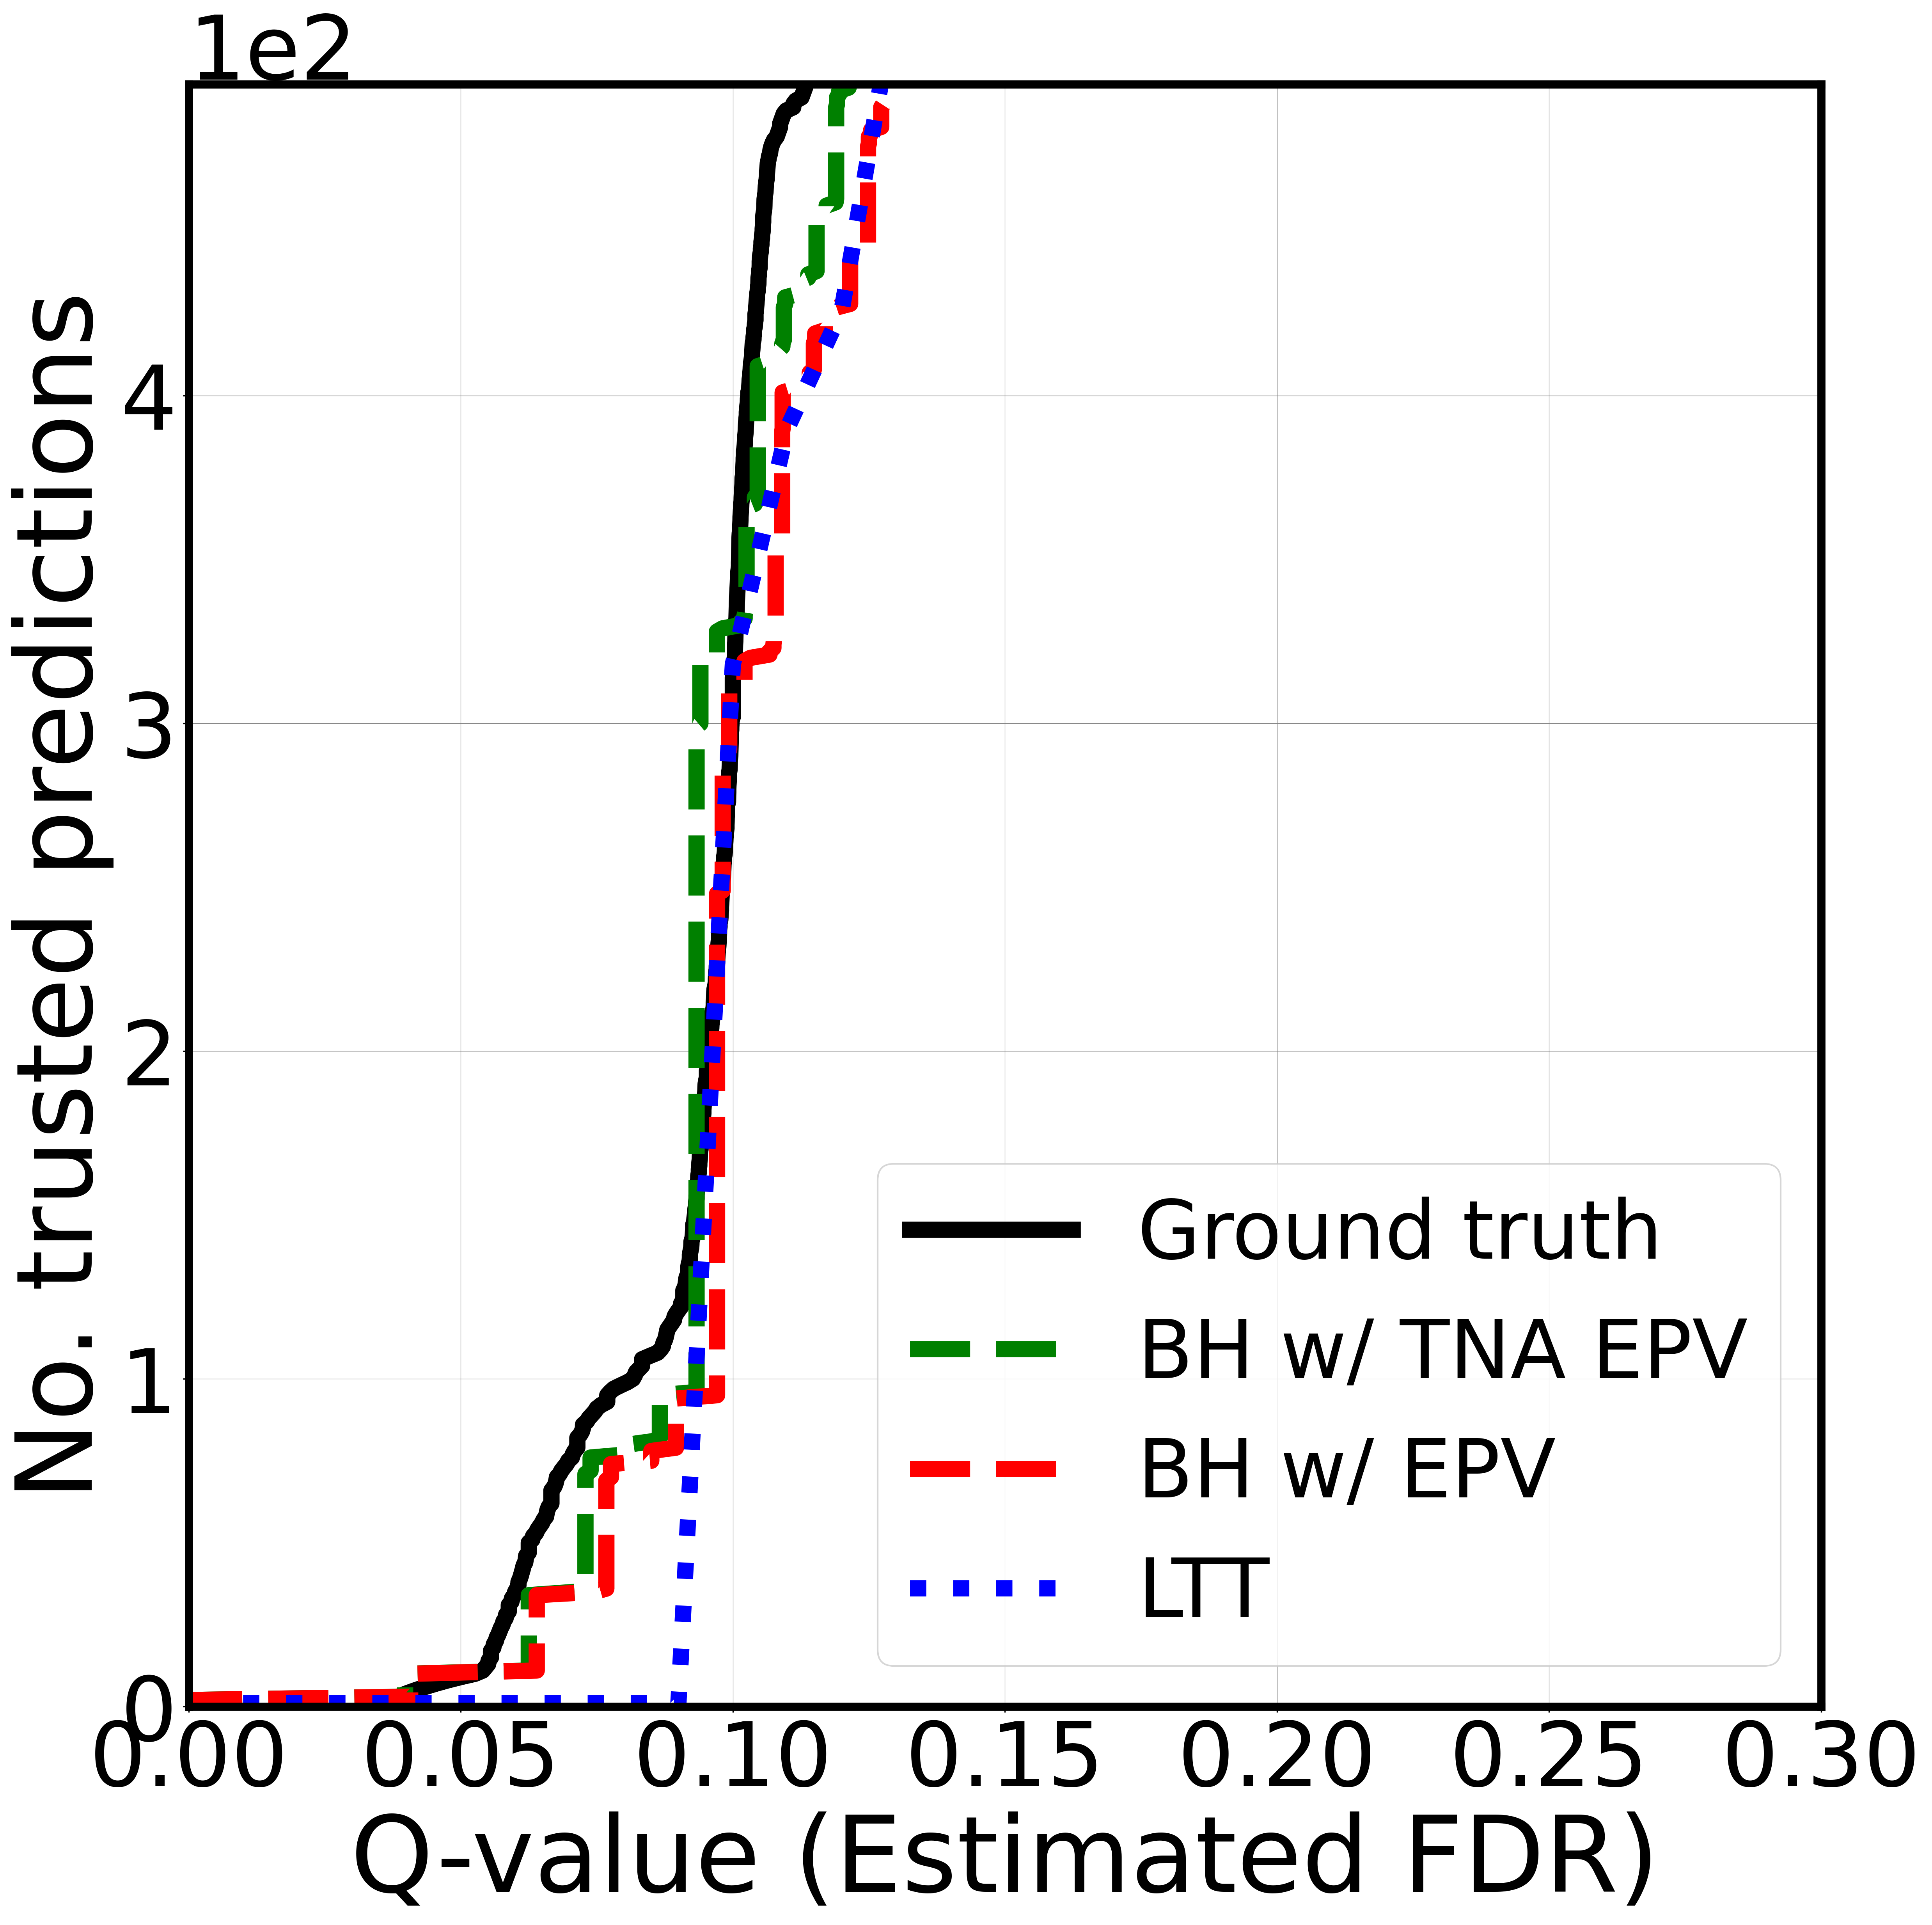
\includegraphics[width=0.225\linewidth, height=0.225\linewidth]{img/cnn_chx_fdr_control_loc.png} & 
		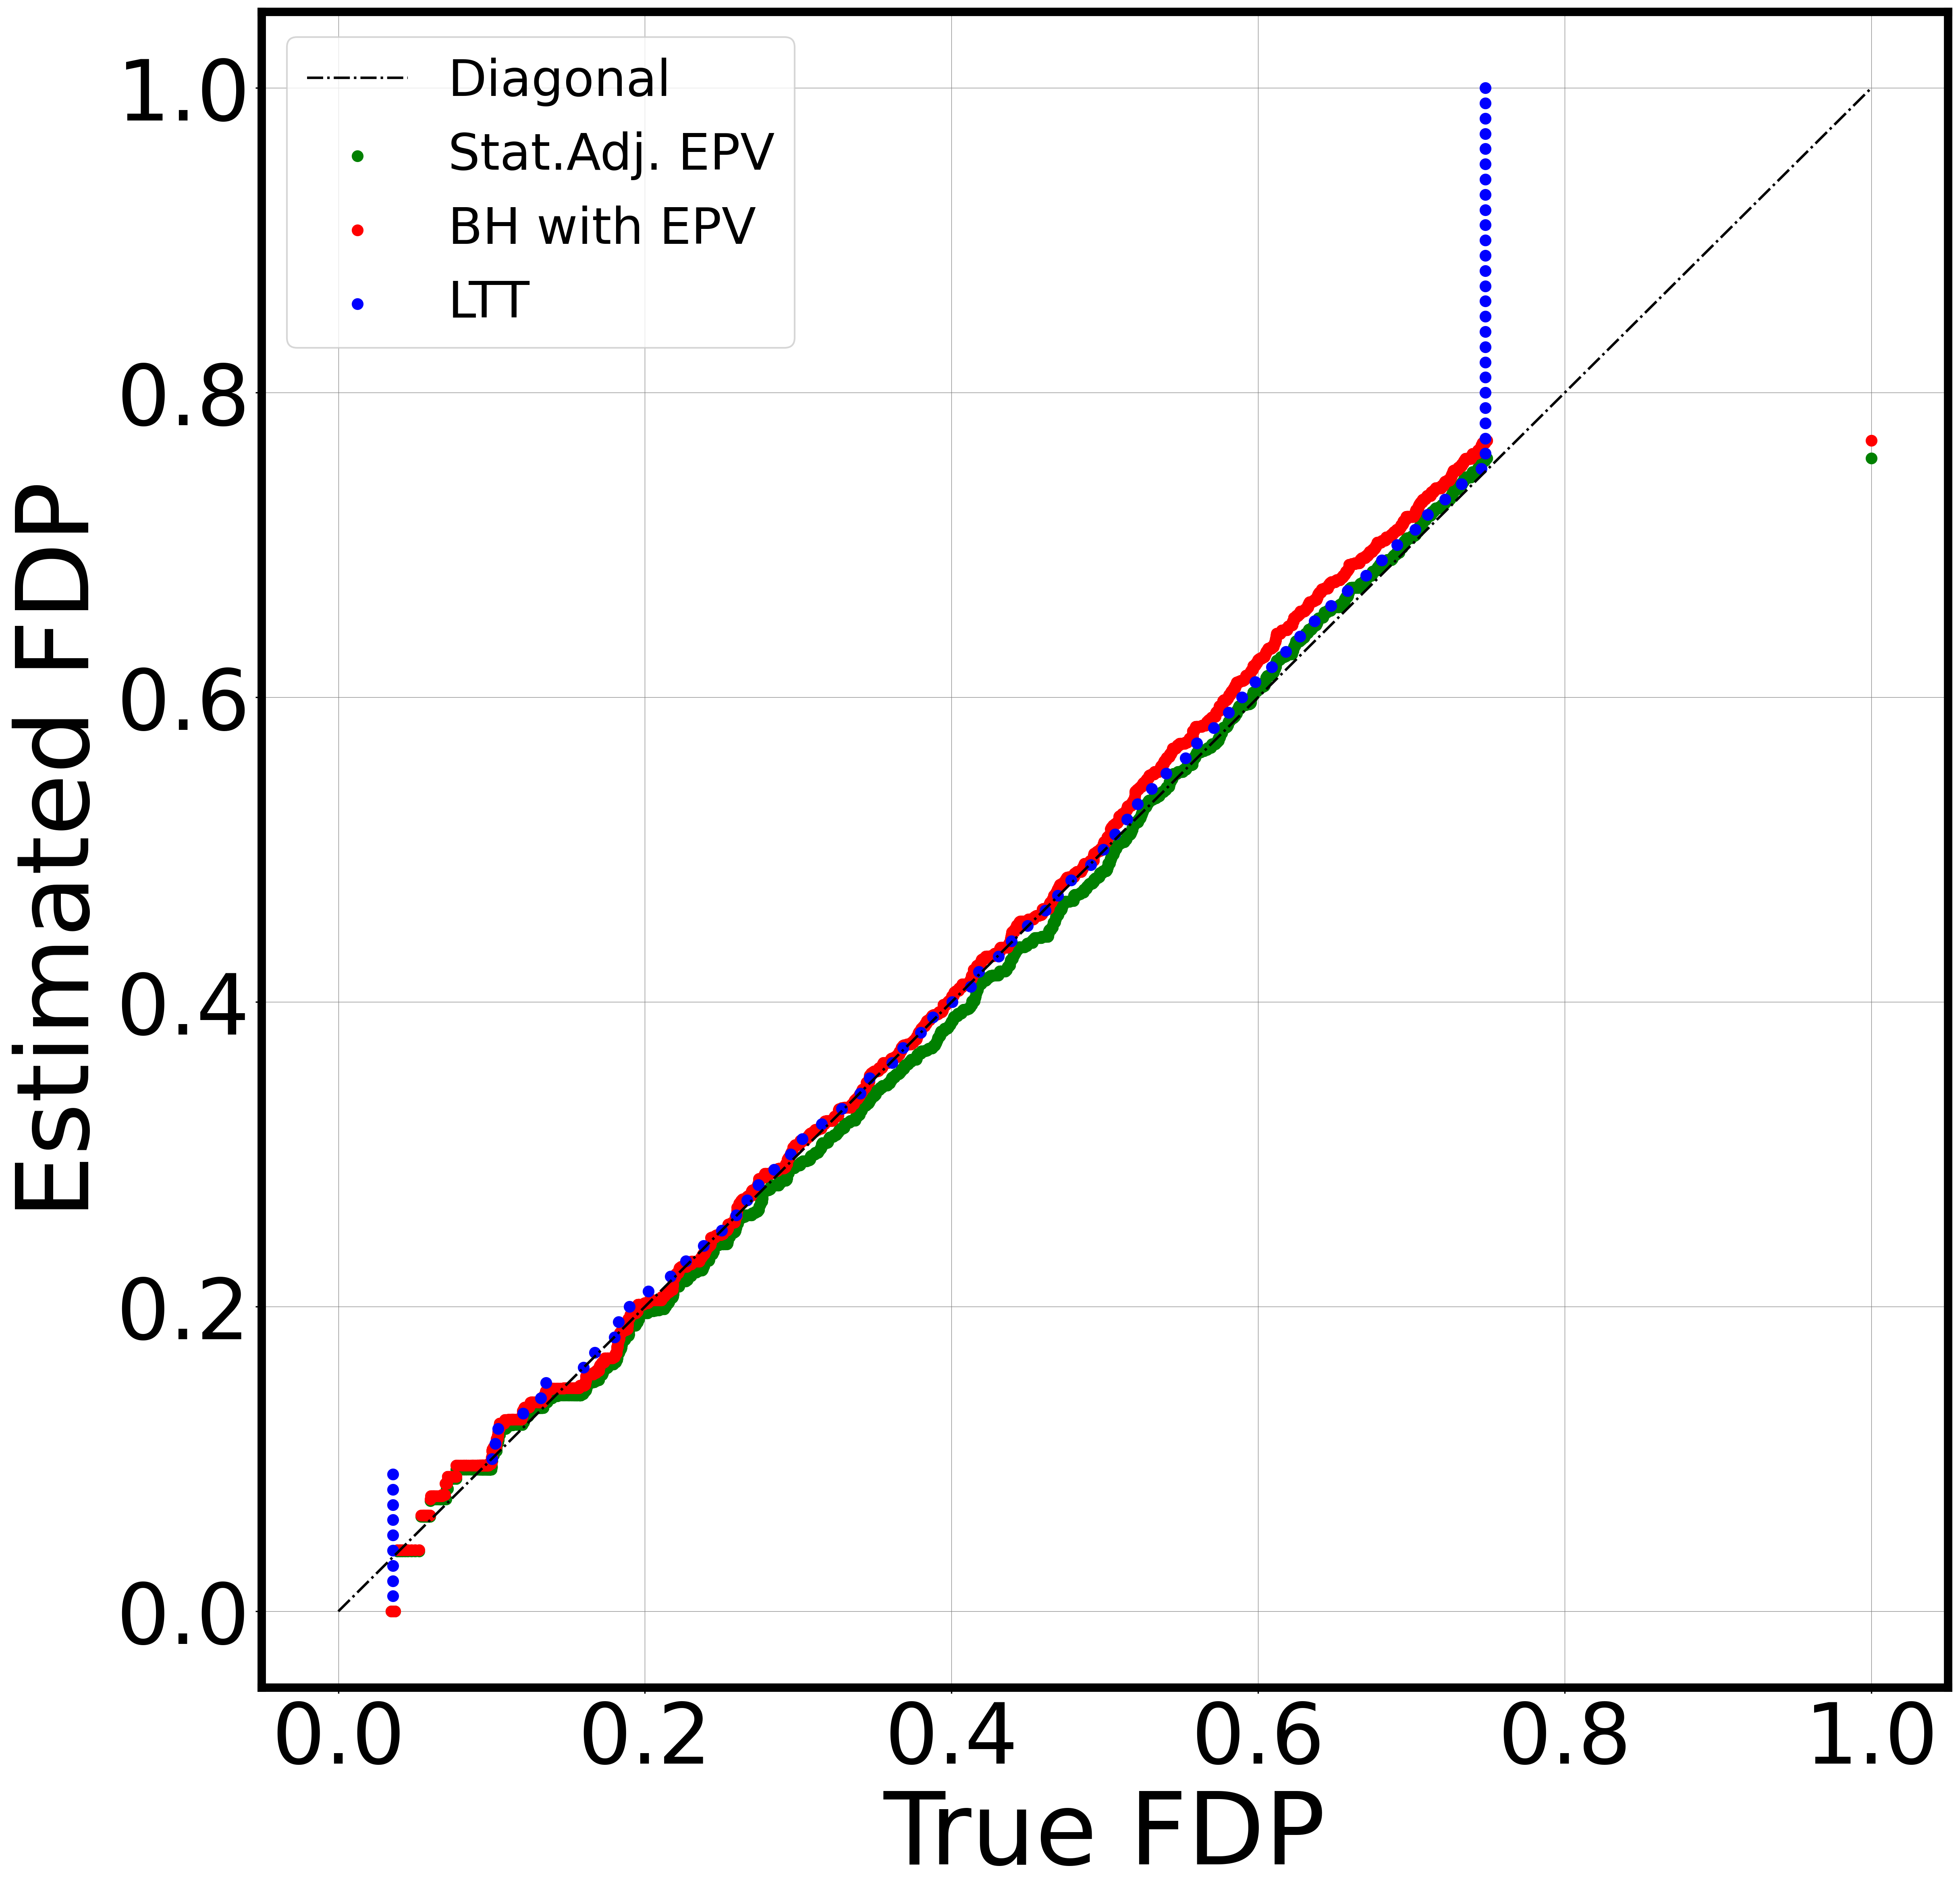
\includegraphics[width=0.225\linewidth, height=0.225\linewidth]{img/cnn_FDPscat_chx.png}\\
		\multicolumn{4}{l}{\bf (iv) CheXpert dataset with class distribution shift:}\\	
		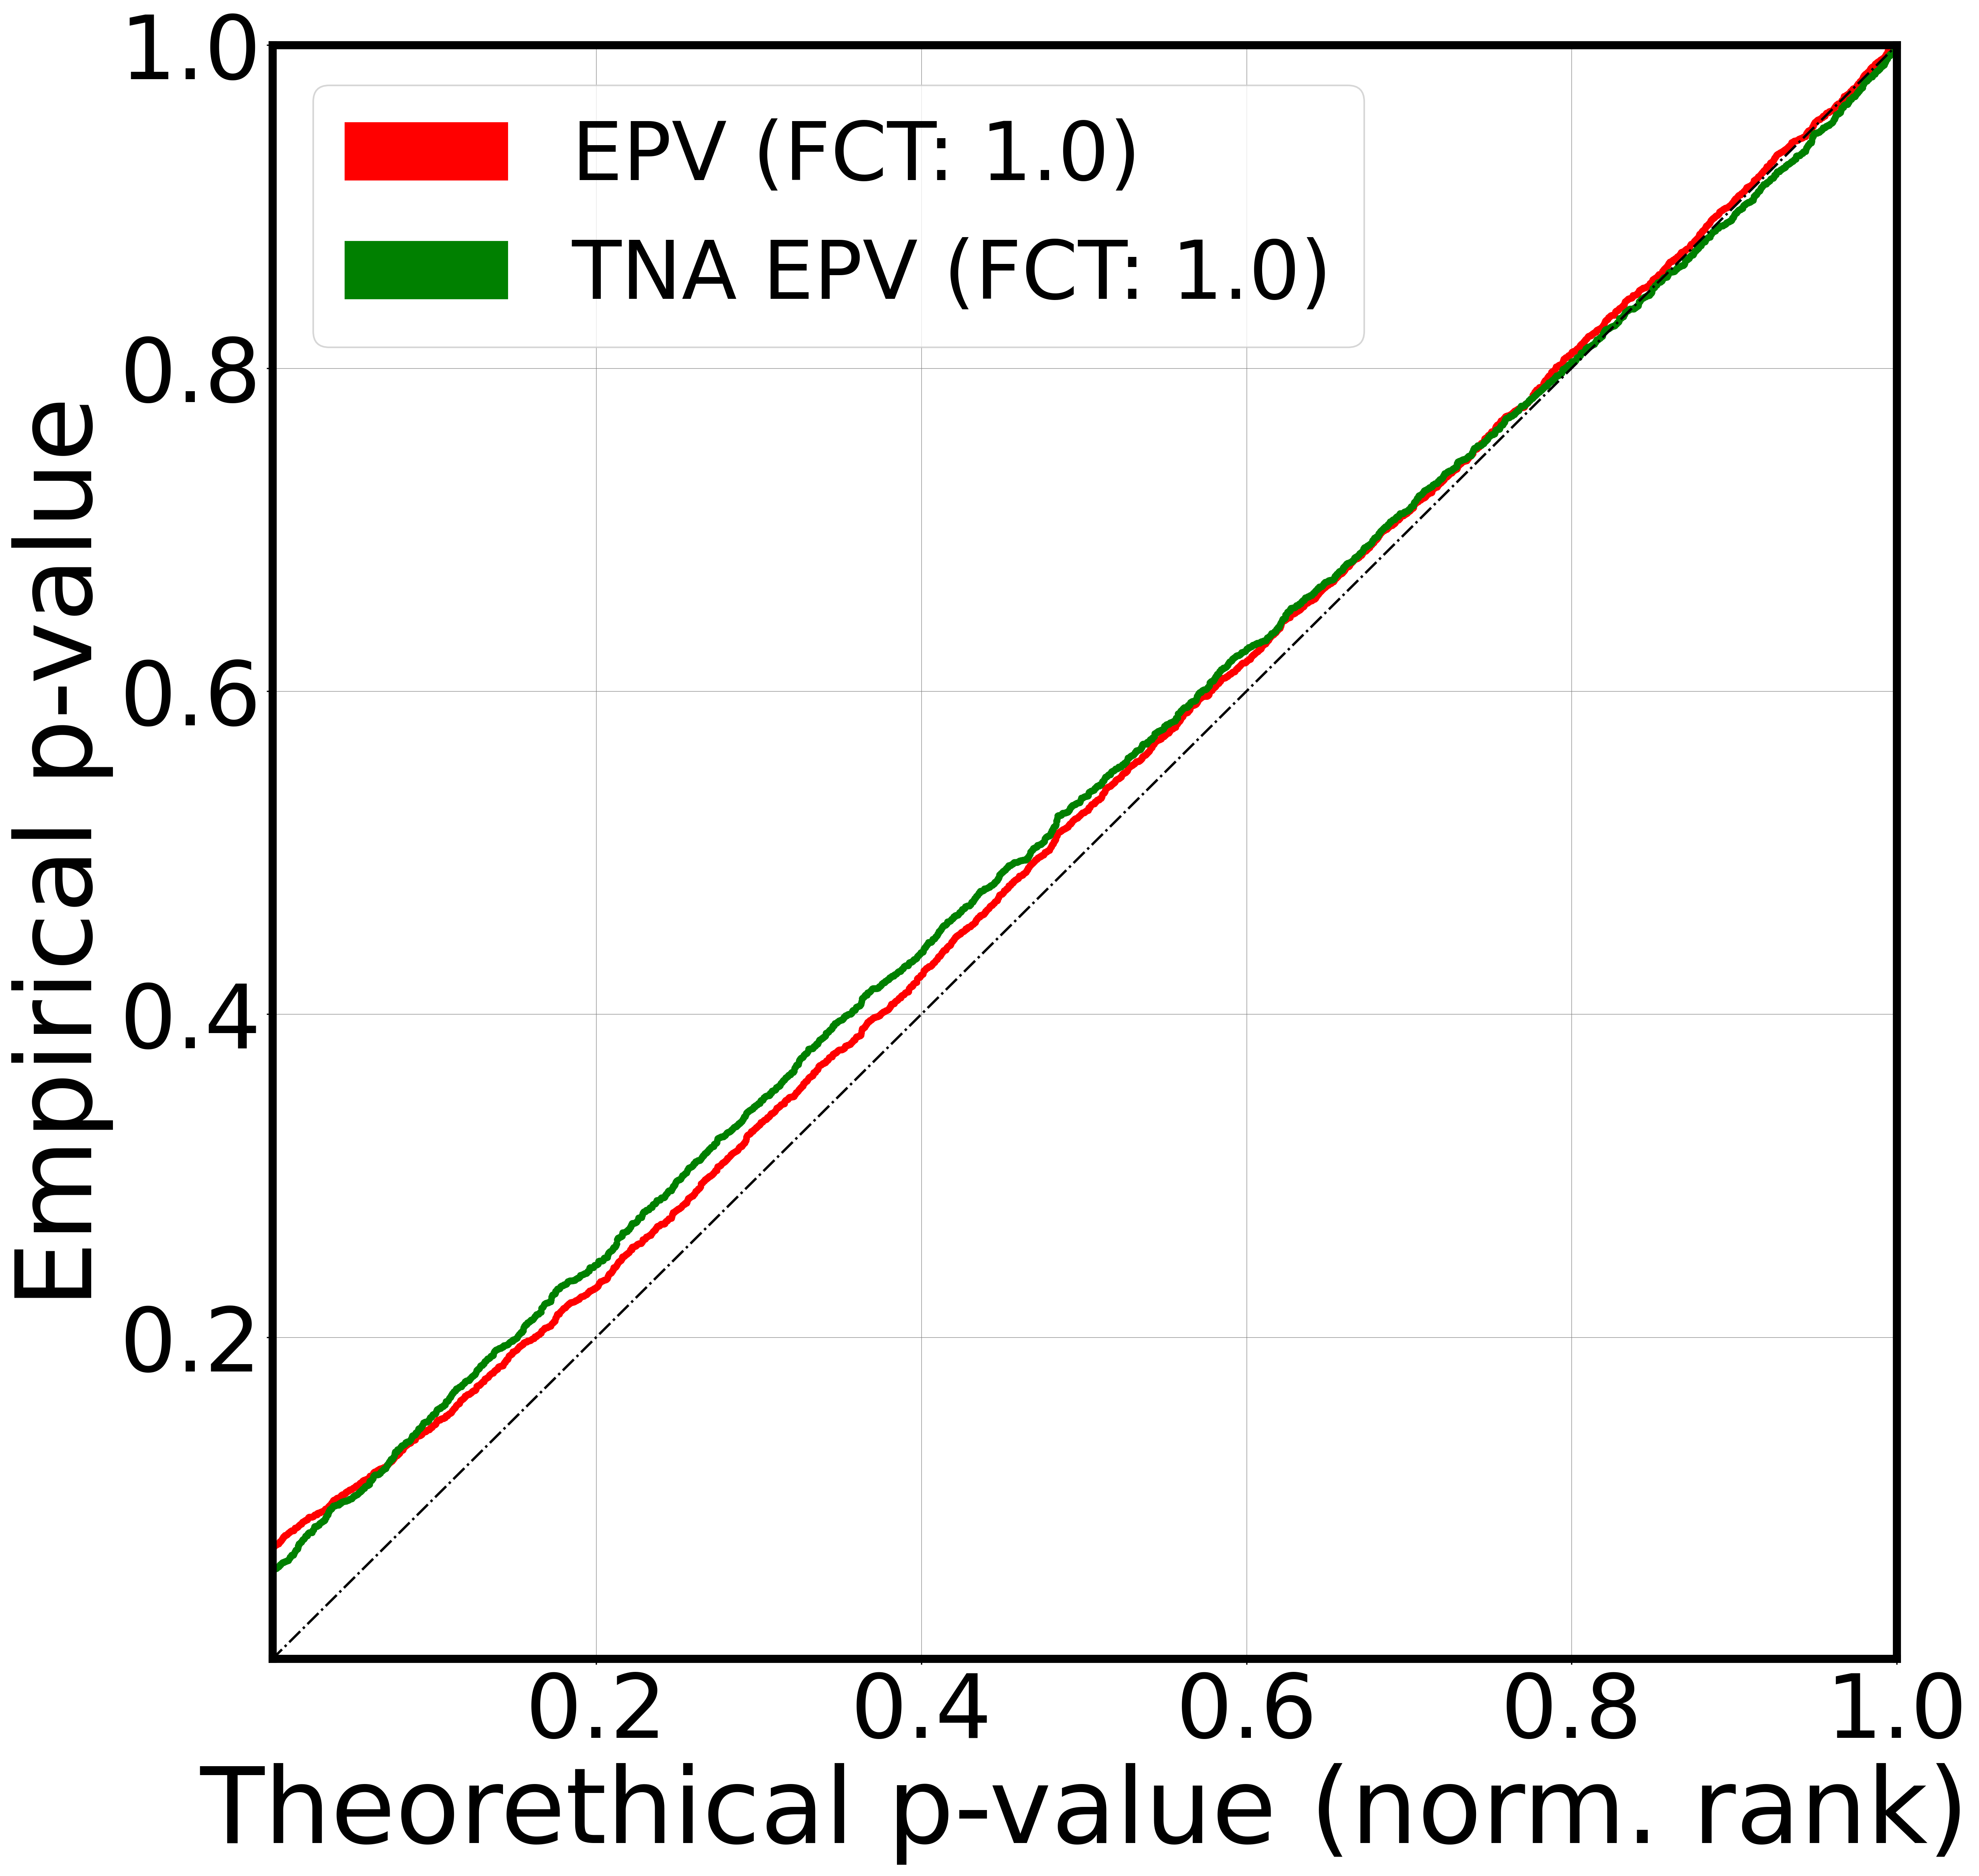
\includegraphics[width=0.225\linewidth, height=0.225\linewidth]{img/cnn_QQ_chx_balanced.png} 		&
		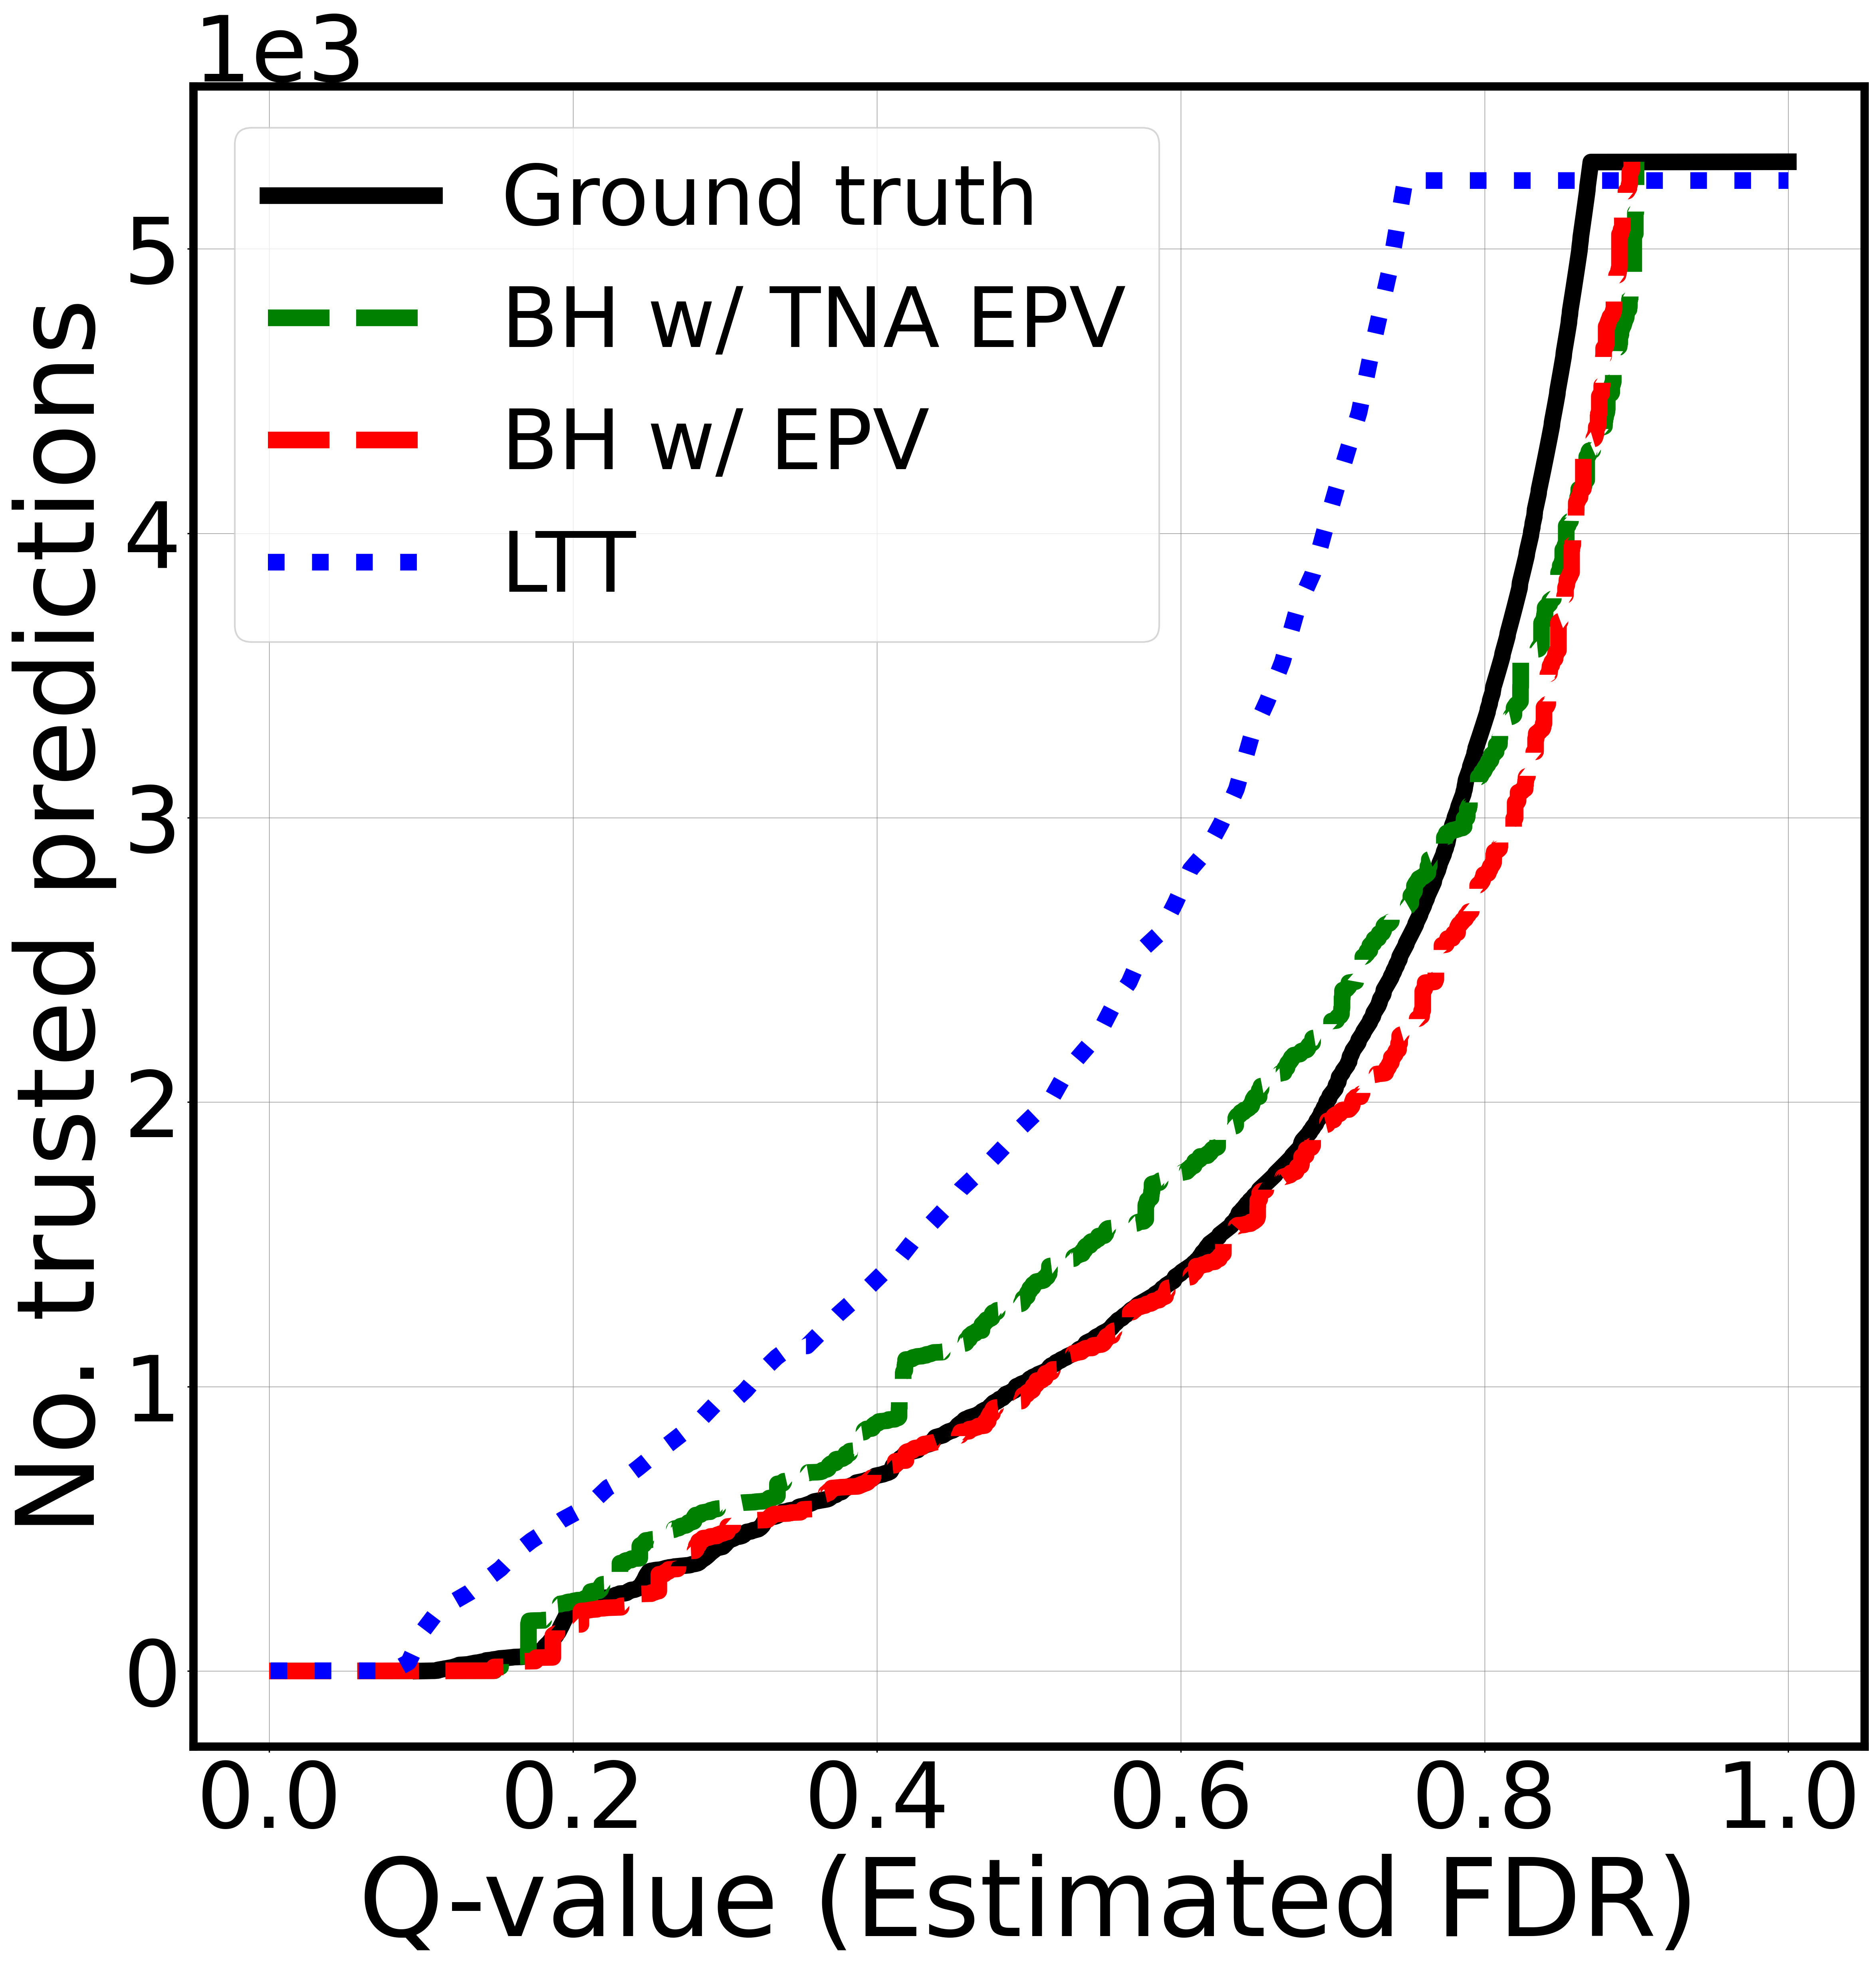
\includegraphics[width=0.225\linewidth, height=0.225\linewidth]{img/cnn_chx_balanced_fdr_control.png} & 
		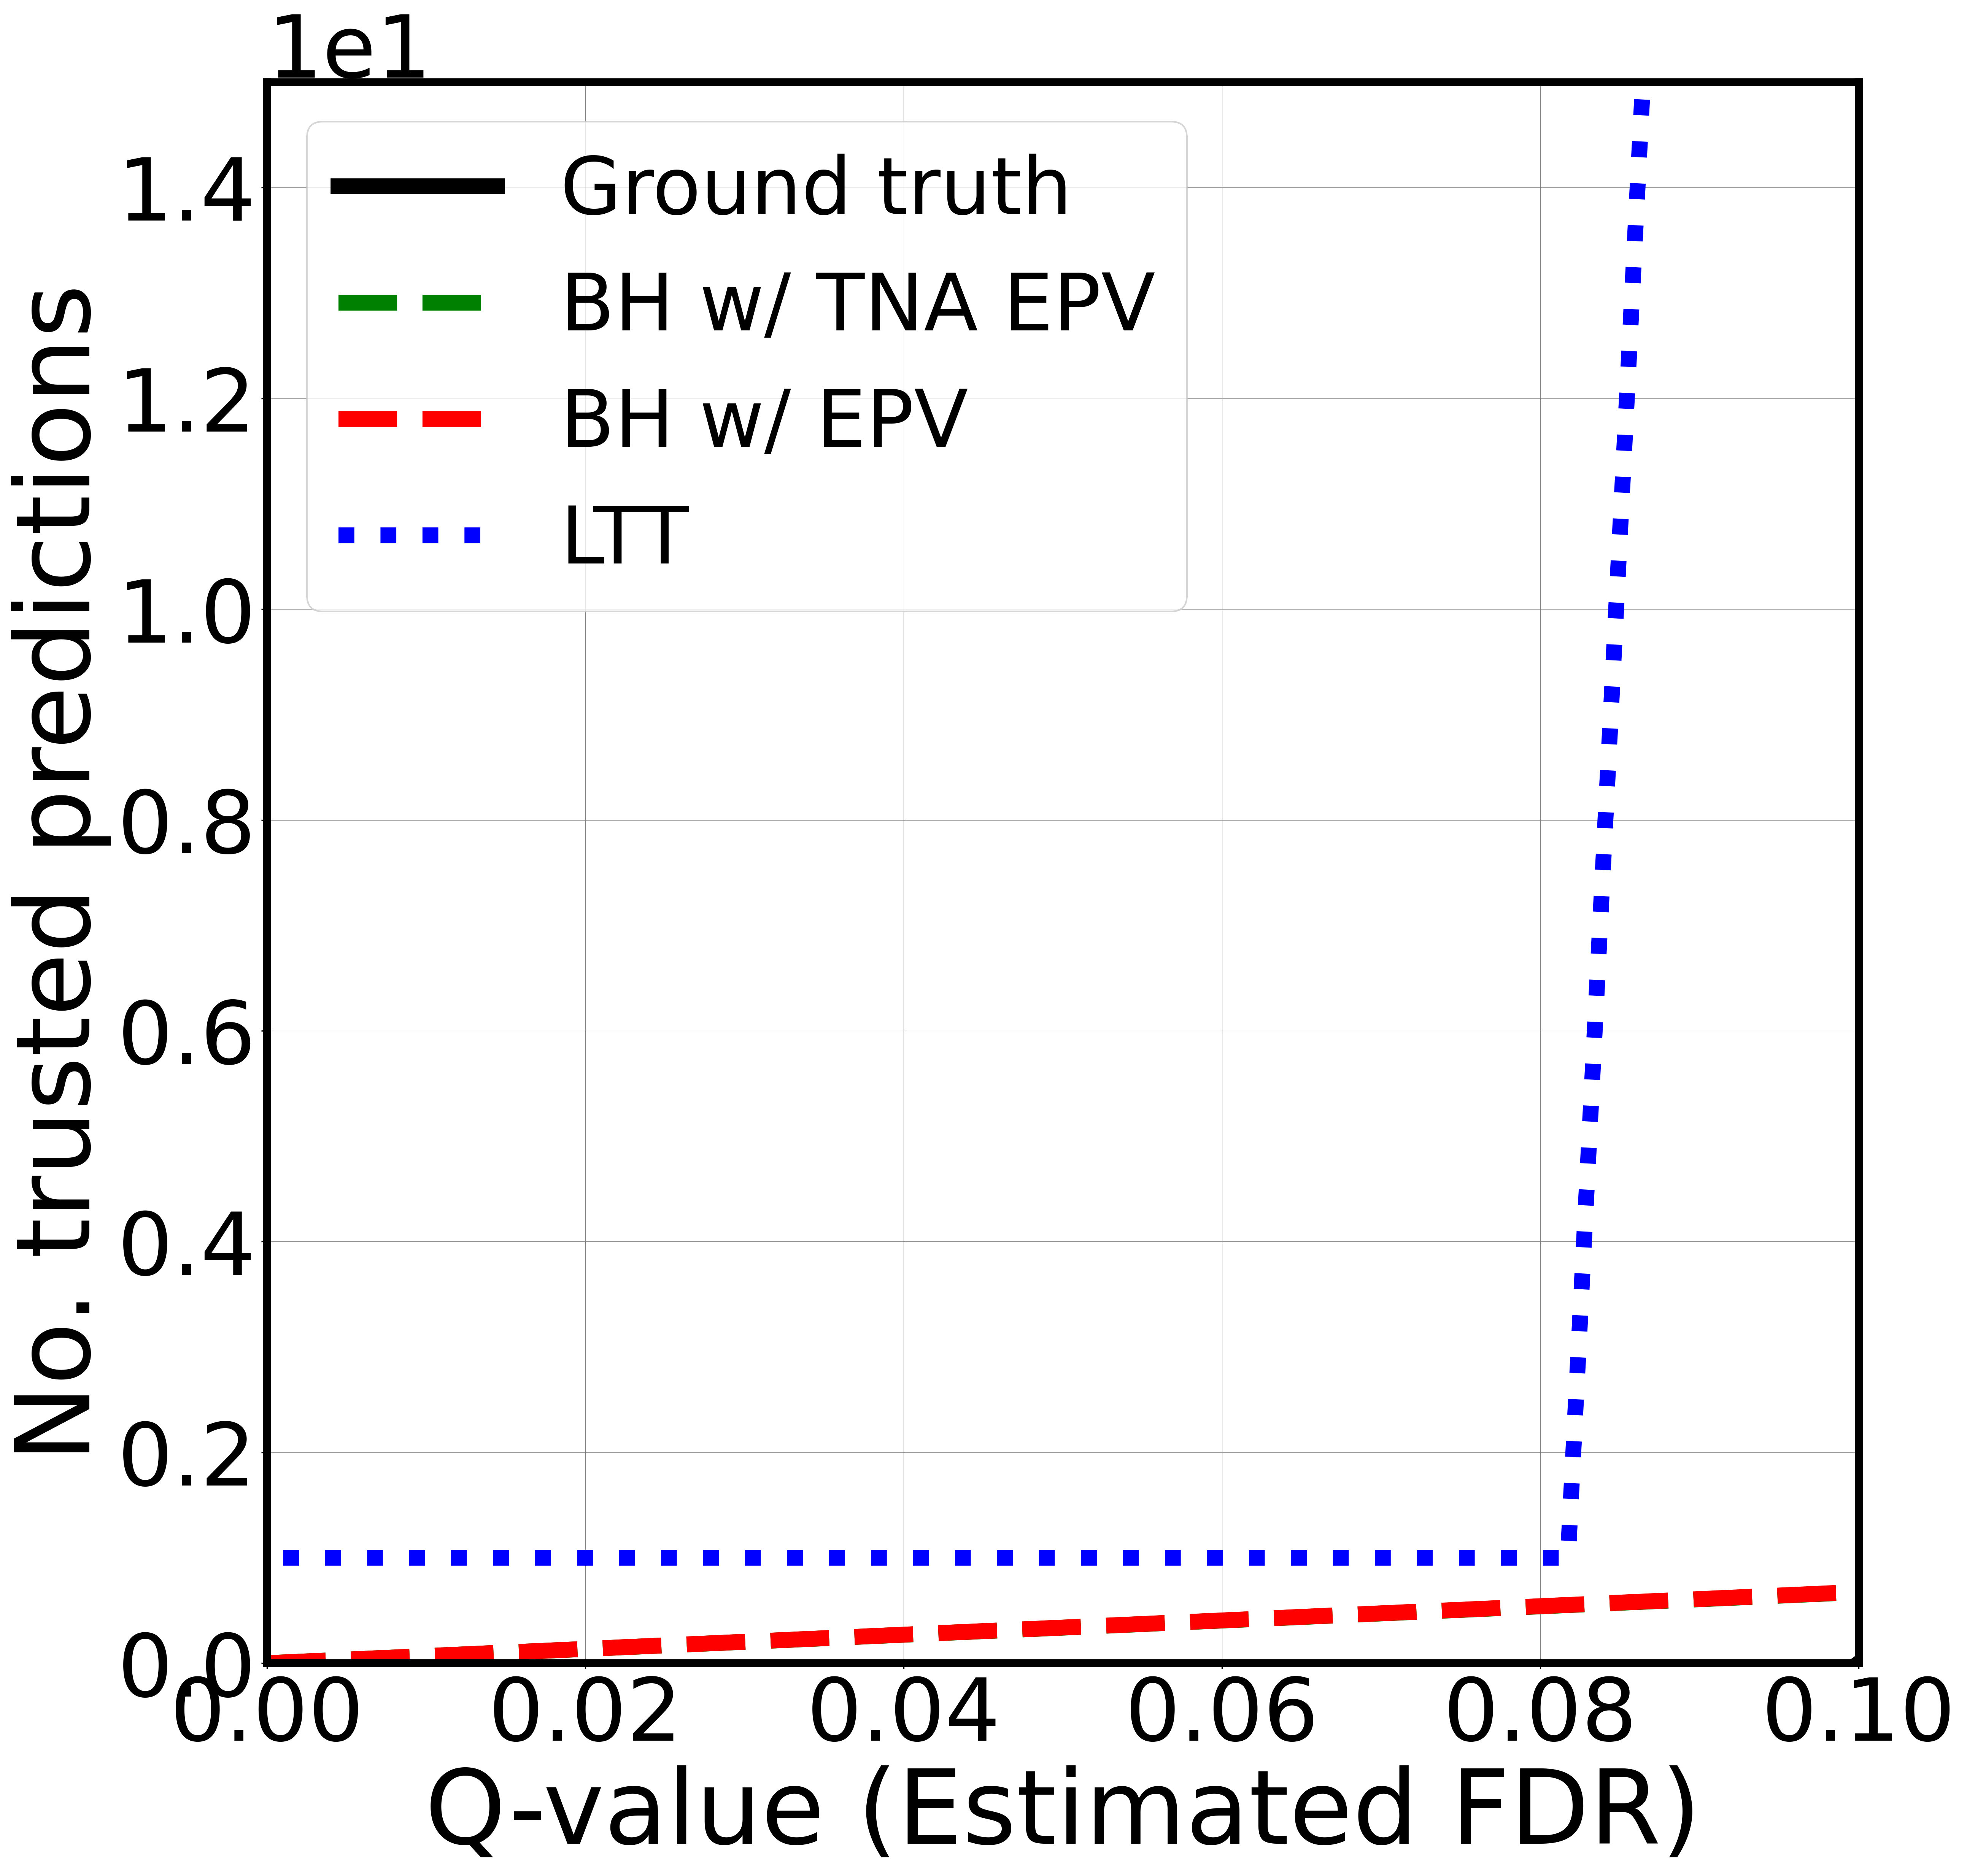
\includegraphics[width=0.225\linewidth, height=0.225\linewidth]{img/cnn_chx_balanced_fdr_control_loc.png} & 
		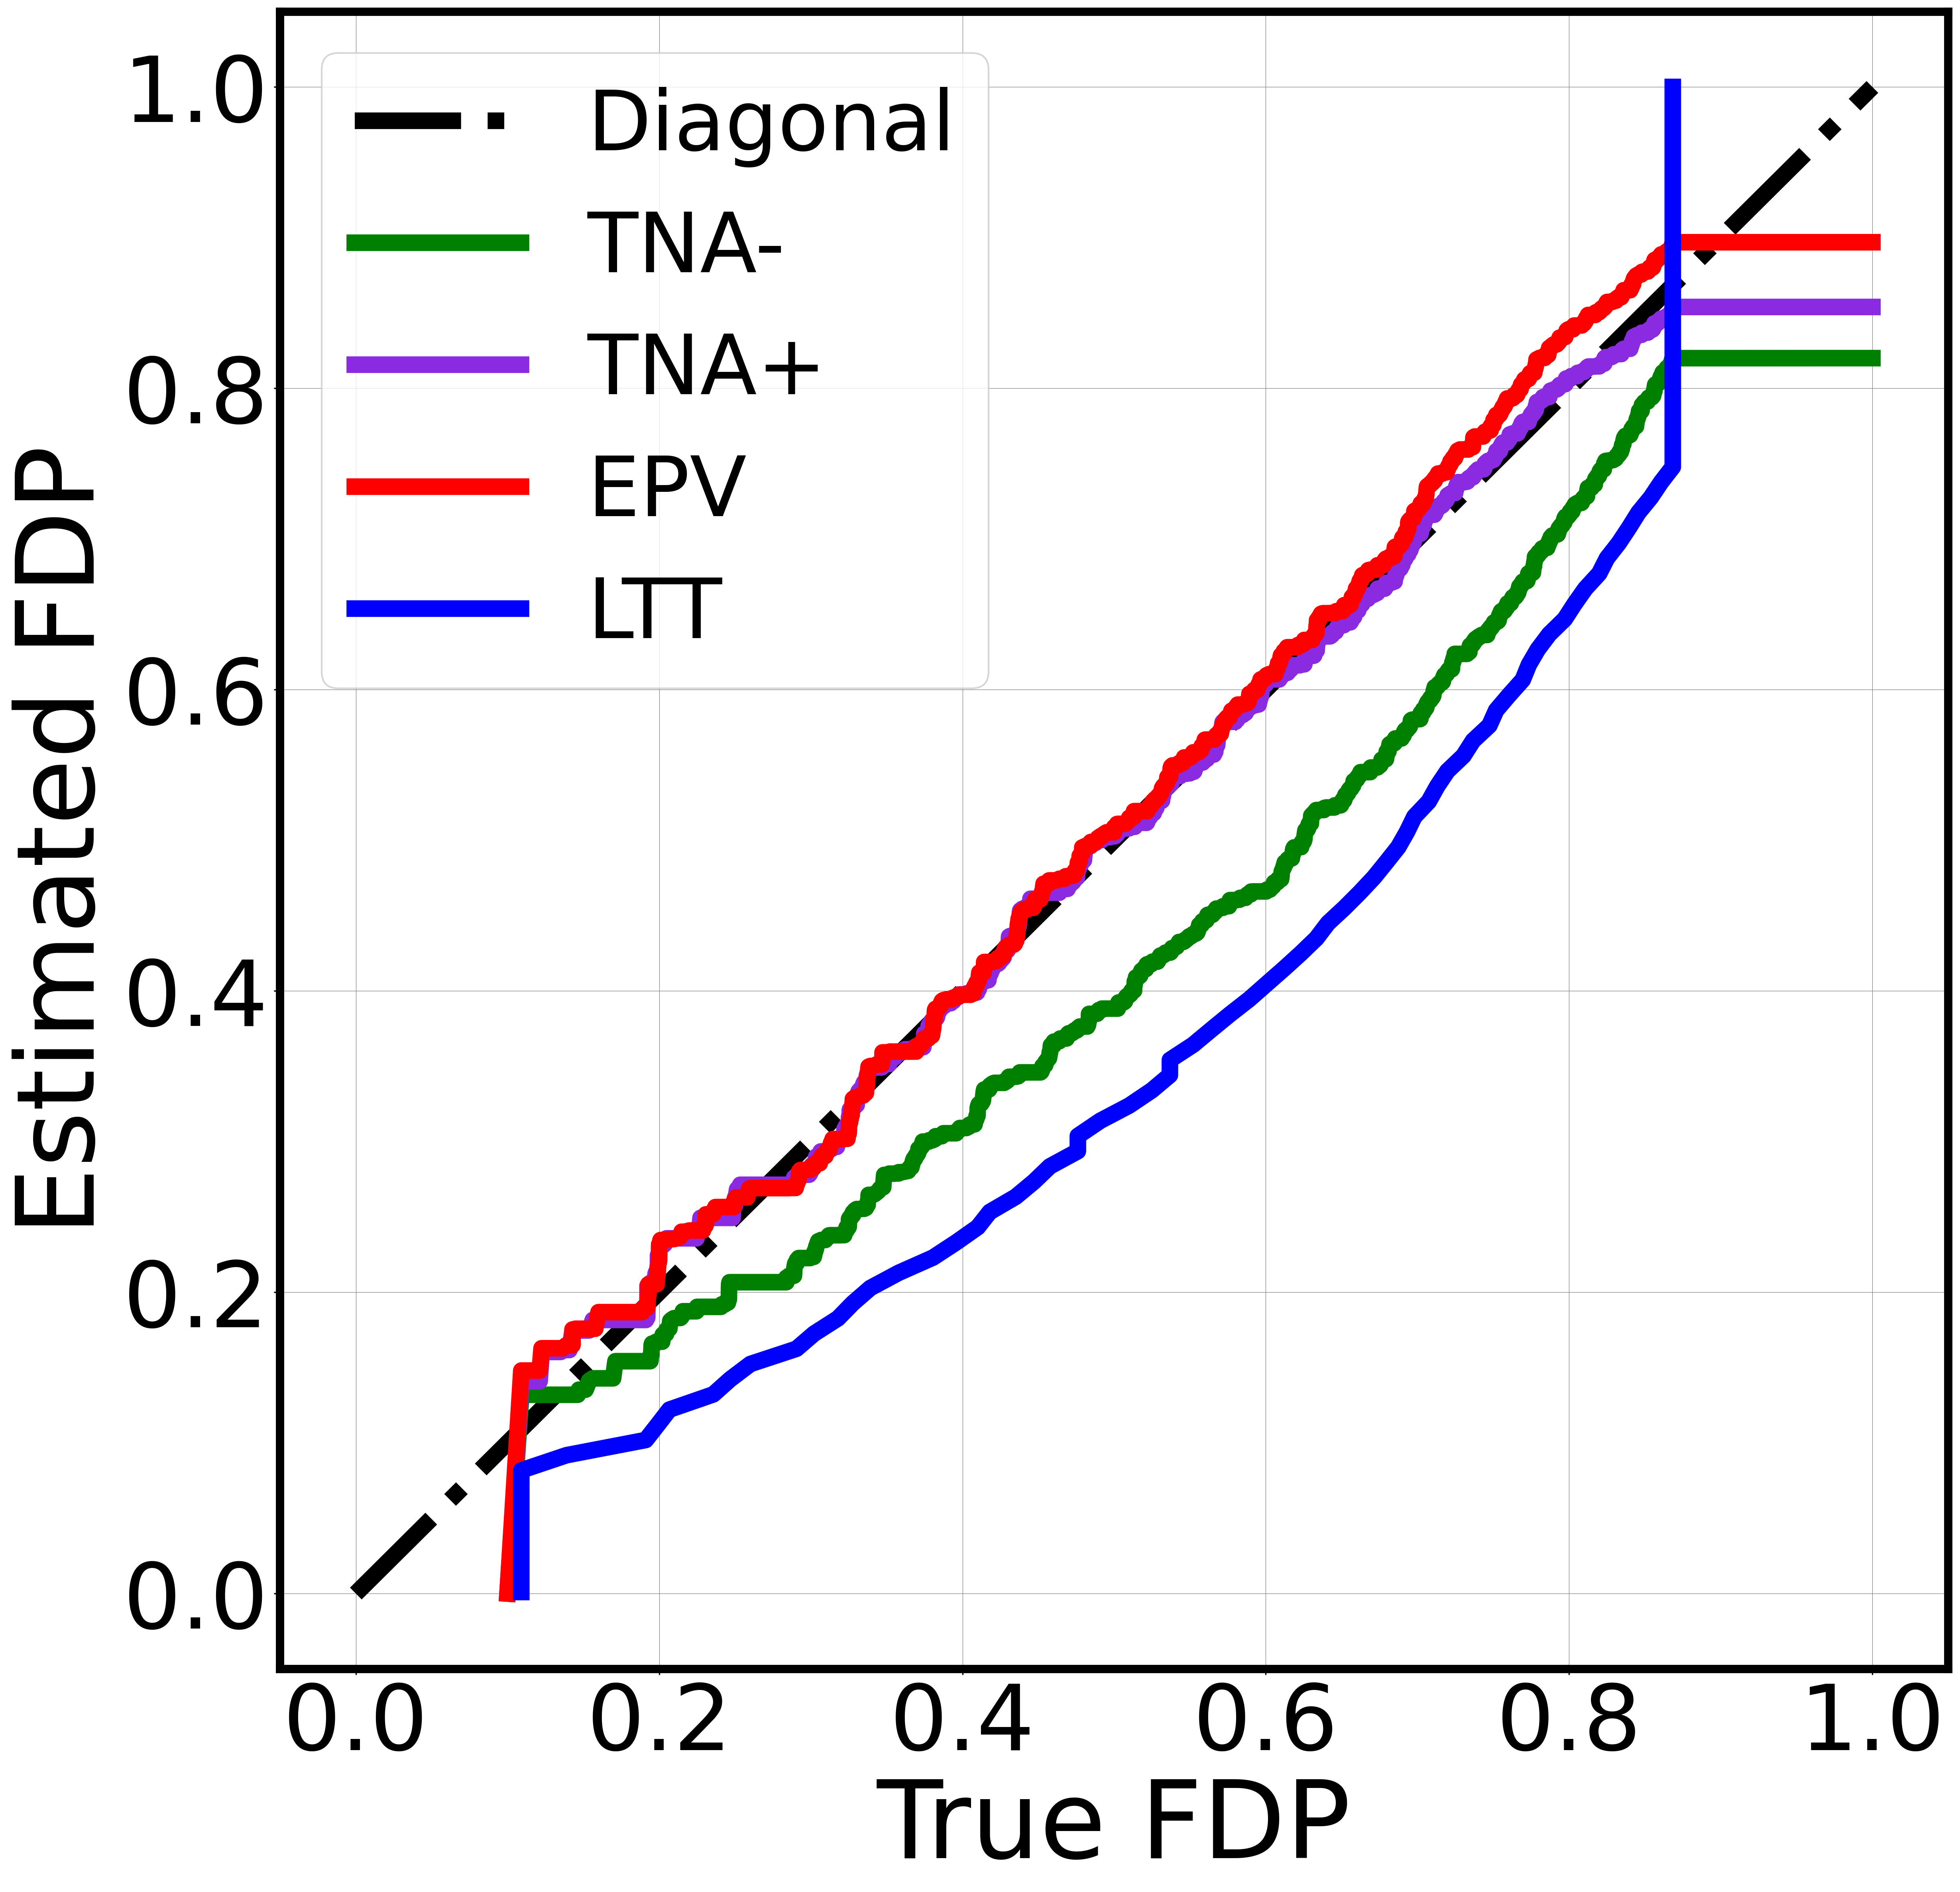
\includegraphics[width=0.225\linewidth, height=0.225\linewidth]{img/cnn_FDPscat_chx_balanced.png}\\
		A & B & C & D
	\end{tabular}
	\caption{{\bf Performance evaluation of FDR controlling methods.} See the caption of Figure \ref{fig:mnist_shfit} for plot descriptions. }
	\label{fig:I}
\end{figure} 

\begin{figure}[h!]
	\centering
	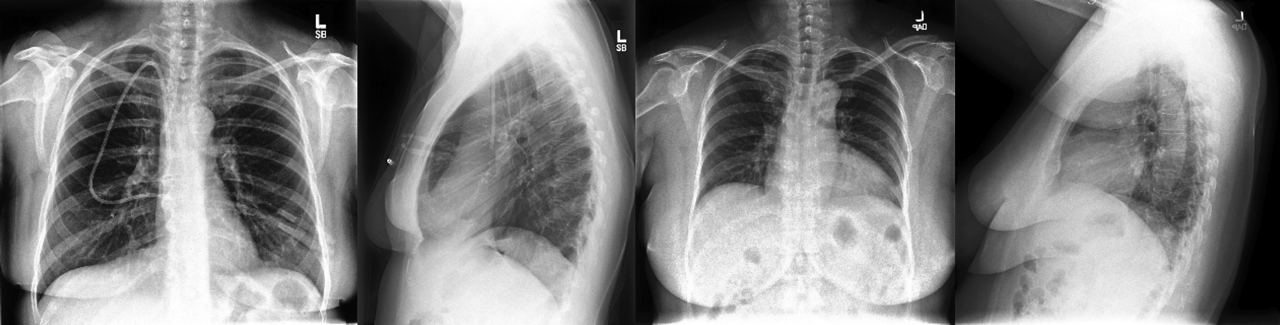
\includegraphics[width=5.in]{img/chx.png}
	\caption{{\bf Instances of CheXpert dataset.}}
	\label{fig:pcam_example}
\end{figure} 

\subsection{CheXpert: chest x-ray dataset}

The CheXpert dataset contains a total of 224,316 radiographs of both frontal and lateral views of the thorax from $\sim$65K patients in order to facilitate the automated interpretation of chest X-rays for multi-label classification tasks (i.e. multiple labels can be predicted for each instances) with a total of 14 labels. We used the deep neural network model, called DenseNet121, from the \texttt{Torchxrayvision} package \cite{cohen2020limits,Cohen2022xrv}, specifically developed for this CheXpert dataset. For the sake of simplicity, we turned the CheXpert dataset into a binary classification task by treating all instances of pleural effusion as positive and all the others as negative. We selected this label because this was the most prevalent  disease in the dataset. The proportion of the positive class became 27 \% and 23 \% in the training and test datasets, respectively. The DenseNet121 model achieved accuracies of 89 \% and 84 \% on the training and test sets, respectively.

We evaluated the four FDR controlling methods and plotted the results on Figure \ref{fig:I}-(iii). Interestingly, the most confident prediction of the DenseNet121 model in the test set is wrong. This can be seen by the flat region of the ground truth evaluation (black line) at low q-values around 0-0.05 (Fig, \ref{fig:I}-(iii)-C). Fortunately, all four FDR controlling methods under investigations managed to capture this and remain close to the ground truth (Fig, \ref{fig:I}-(iii)-B-D). The standard EPVs (red dots) tend to be off at the critical range (p-value $<$ 0.1), but this does not affect the FDR controlling results in this benchmark, perhaps because of the confident incorrect predictions. Overall, we conclude that all four methods provide accurate FDR control. In our opinion, this indicates the absence of any database distribution shits. These plots also show that our TNA- and TNA+ algorithms do not corrupt  the EPVs in the absence of data shift.

The actual frequency of pleural effusion may be different among all chest x-ray radiographs performed. It may vary over locations, age groups, in-patients and out-patients \cite{Zaki2024,Cashen2017PleuralEA}. In the United States, 275 million conventional radiology procedures are performed annually \cite{mahesh2022patient}, but only around 1.5 million of US citizens develop pleural effusion \cite{Cashen2017PleuralEA}. Pleural effusion develops in about 20-40\% of in-patient with pneumonia \cite{shebl2018parapneumonic}. Whatever the real abundance of the pleural effusion is among  chest x-rays performed, it can be significantly different from the 27 \% of the CheXpert dataset. Taking this into account, we re-sampled the test set in the CheXpert dataset to achieve a lower positive class ratio of 13\%. The results of the re-evaluation are shown in Figure \ref{fig:I}-(iv). The LTT and the TNA- EPVs are both slightly biased. The BH with the standard EVPs and with TNA+ EPVs achieve the most accurate FDR control over the entire range of $\alpha$ levels (0-1) in general. The LTT method is very sensitive to class distribution shift demonstrated by this case, wheree it resulted in a liberally biased FDR control.



\subsection{TissueNet: cells segmentation}

\begin{figure}[h!]
    \centering
	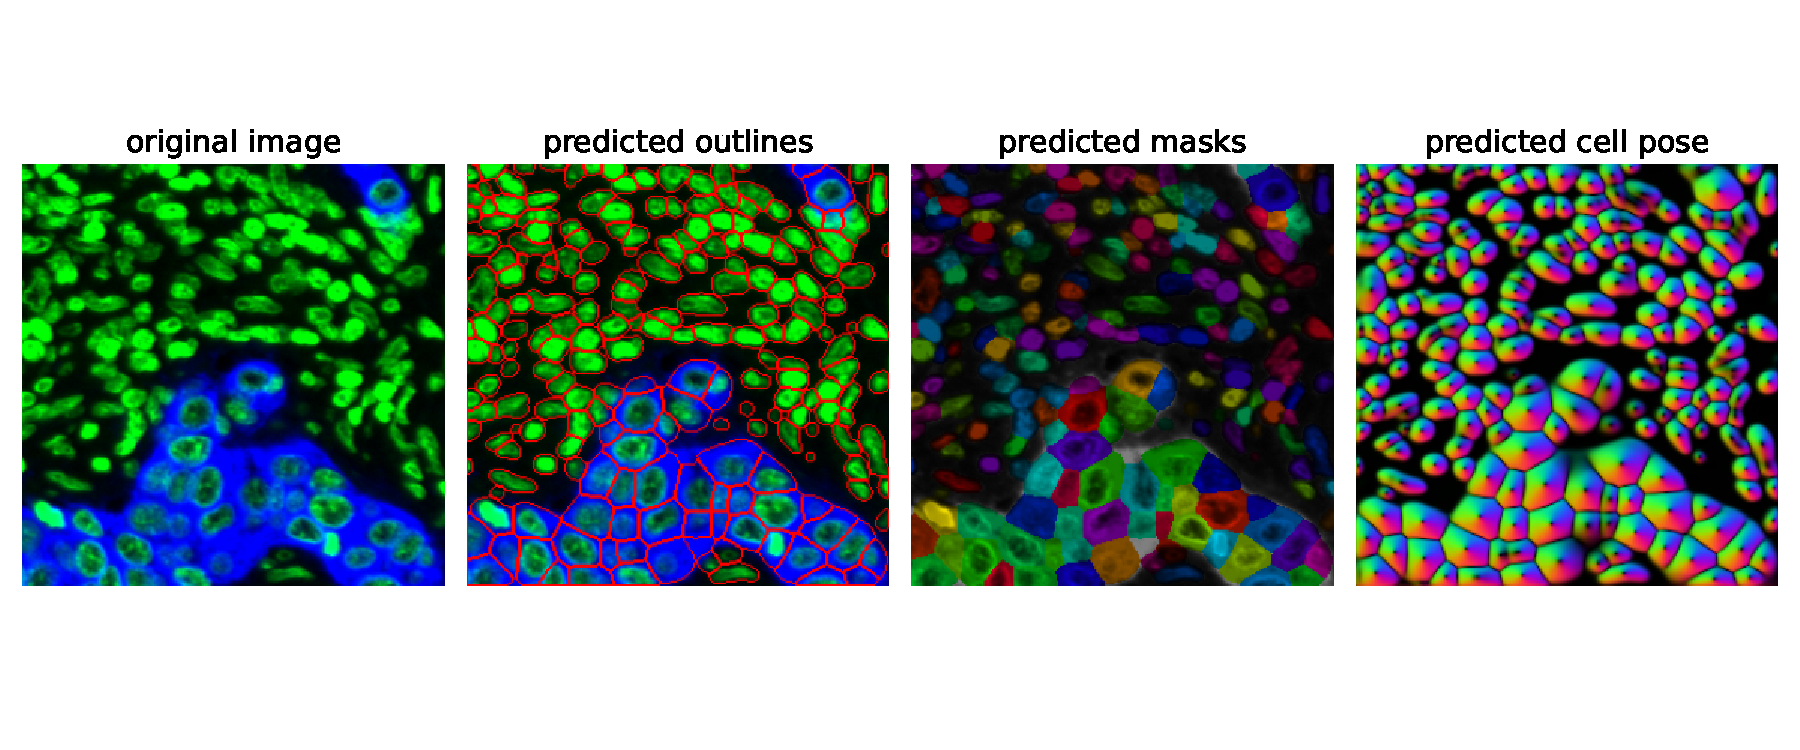
\includegraphics[width=5in]{img/tissuenet.pdf}
	\caption{{\bf Instance of TissueNet dataset.} Two-channel original images are being processed by the model, in turn producing masks \& flows to correctly segment cells}
	\label{fig:tissue_example}
\end{figure} 

TissueNet dataset contains 1.3 million microscopic images of cells obtained from six various platforms and nine organs including both histologically healthy and diseased tissues. Each images has size of 512x512 pixels, was manually segmented at pixel level and paired whole-cell and nuclear annotations. Our binary classification task was to predict whether a pixel is inside a cell (positive) or not (negative). The overall positive-negative ratio was 59\%:41\% in the training data and in contrast to 66\%:34\% in the test data. However, the class ratio varies over the images considerably. We used the Cellpose pre-trained deep neural network model \cite{cellpose} and fine-tuned it for five epochs. It achieved accuracy of 95\% and 94\% on training and test data, respectively. Our evaluation is reported in Figure \ref{fig:ii}-(i). The plots reveal that the BH protocol with standard EPVs becomes liberally biased (Fig. \ref{fig:ii}-(i)-B-C). The latter possibly originates from the data distribution shift or from overfitting. Both LTT and the BH with TNA EPV remain accurate. 

The situation changes when we evaluate the segmentation problem with a single image. We arbitrarily chose one test image (ID: 007-008-009) and run the Cellpose model to classify each pixel. The positive and negative class balance was: 33\%:67\%. The Q-Q plot (Fig. \ref{fig:ii}-(ii)-A) of the test EPVs (red dots) indicates that the scores of negative samples from training and test datasets are different. The TNA EPVs on the Q-Q plot shows that the TNA methods have managed to adjust the p-values of the test samples (green and purple dots) closer to the uniform distribution. The plots on Fig. \ref{fig:ii}-(ii)-B-D indicate that LTT has turned out to be liberally biased, the BH method with standard EPVs strongly conservative. The BH with TNA- EPVs (green) and with TNA+ EPVs (purple) remain accurate in the critical region of q-values (0-0.4). Thus, the TNA methods have succeeded in correcting the p-values at the critical range at least. 






\subsection{BCSS: Breast cancer semantic segmentation dataset}

\begin{figure}[h!]
	\centering
	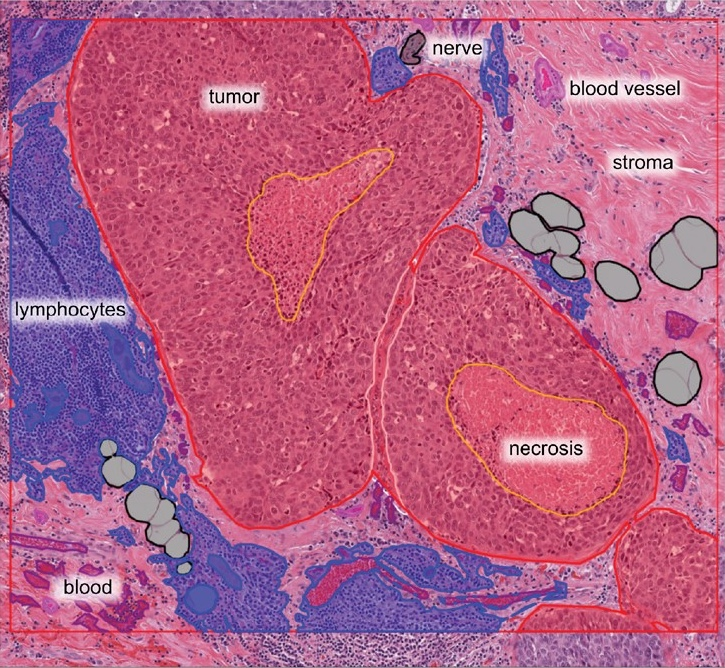
\includegraphics[width=3in]{img/bcss_instance.jpeg}
	\caption{{\bf An instance from BCSS dataset.}}
	\label{fig:bcss_example}
\end{figure} 

The Breast Cancer Semantic Segmentation (BCSS) dataset \cite{Amgad2019StructuredCE} contains around 20K image segmentation objects annotated through Digital Slide Archive, with a particular focus on tissue regions derived from breast cancer imagery obtained from The Cancer Genome Atlas (TCGA). The image pixels are labeled by: 'Stroma' (class id: 0), 'Tumor' (class id: 1) and 'Others' (class id: 2). The corresponding class ratios in the training and test sets are 56\%:38\%:6\% and 33\%:59\%:8\%, respectively. We used the deep learning model called \texttt{'fcn resnet50 unet-bcss'} from the TIA (Tissue Image Analysis) toolbox \cite{Pocock2022} to classify the pixels to one of the three classes. The model achieved an accuracy of 84 \% and 82 \% on the training and test datasets, respectively. 

Since this dataset involves a multi-class classification problem, we slightly modified the FDR control procedure. We calculated the p-values, the $\pi_0$ estimations with Storey method with respect to a single class (deemed as positive); thus, for each pixels, we got three p-values, each corresponding to one of the three classes. Then we concatenated all of these p-values and calculated the q-values. We note that, we did not evaluate LTT on this benchmark, because it is not clear how to adjust it to multi-class classification problems.



%Our conclusion with this benchmark datasets is that the deviations in QQ plots and sharp turns in the plot of trusted predictions (without the ground truth) should be alarming to researchers about the performance of their models. 

\begin{figure}
	\centering
	\begin{tabular}{cccc}
		\multicolumn{4}{l}{\bf (i) Standard TissueNet dataset:}\\		
		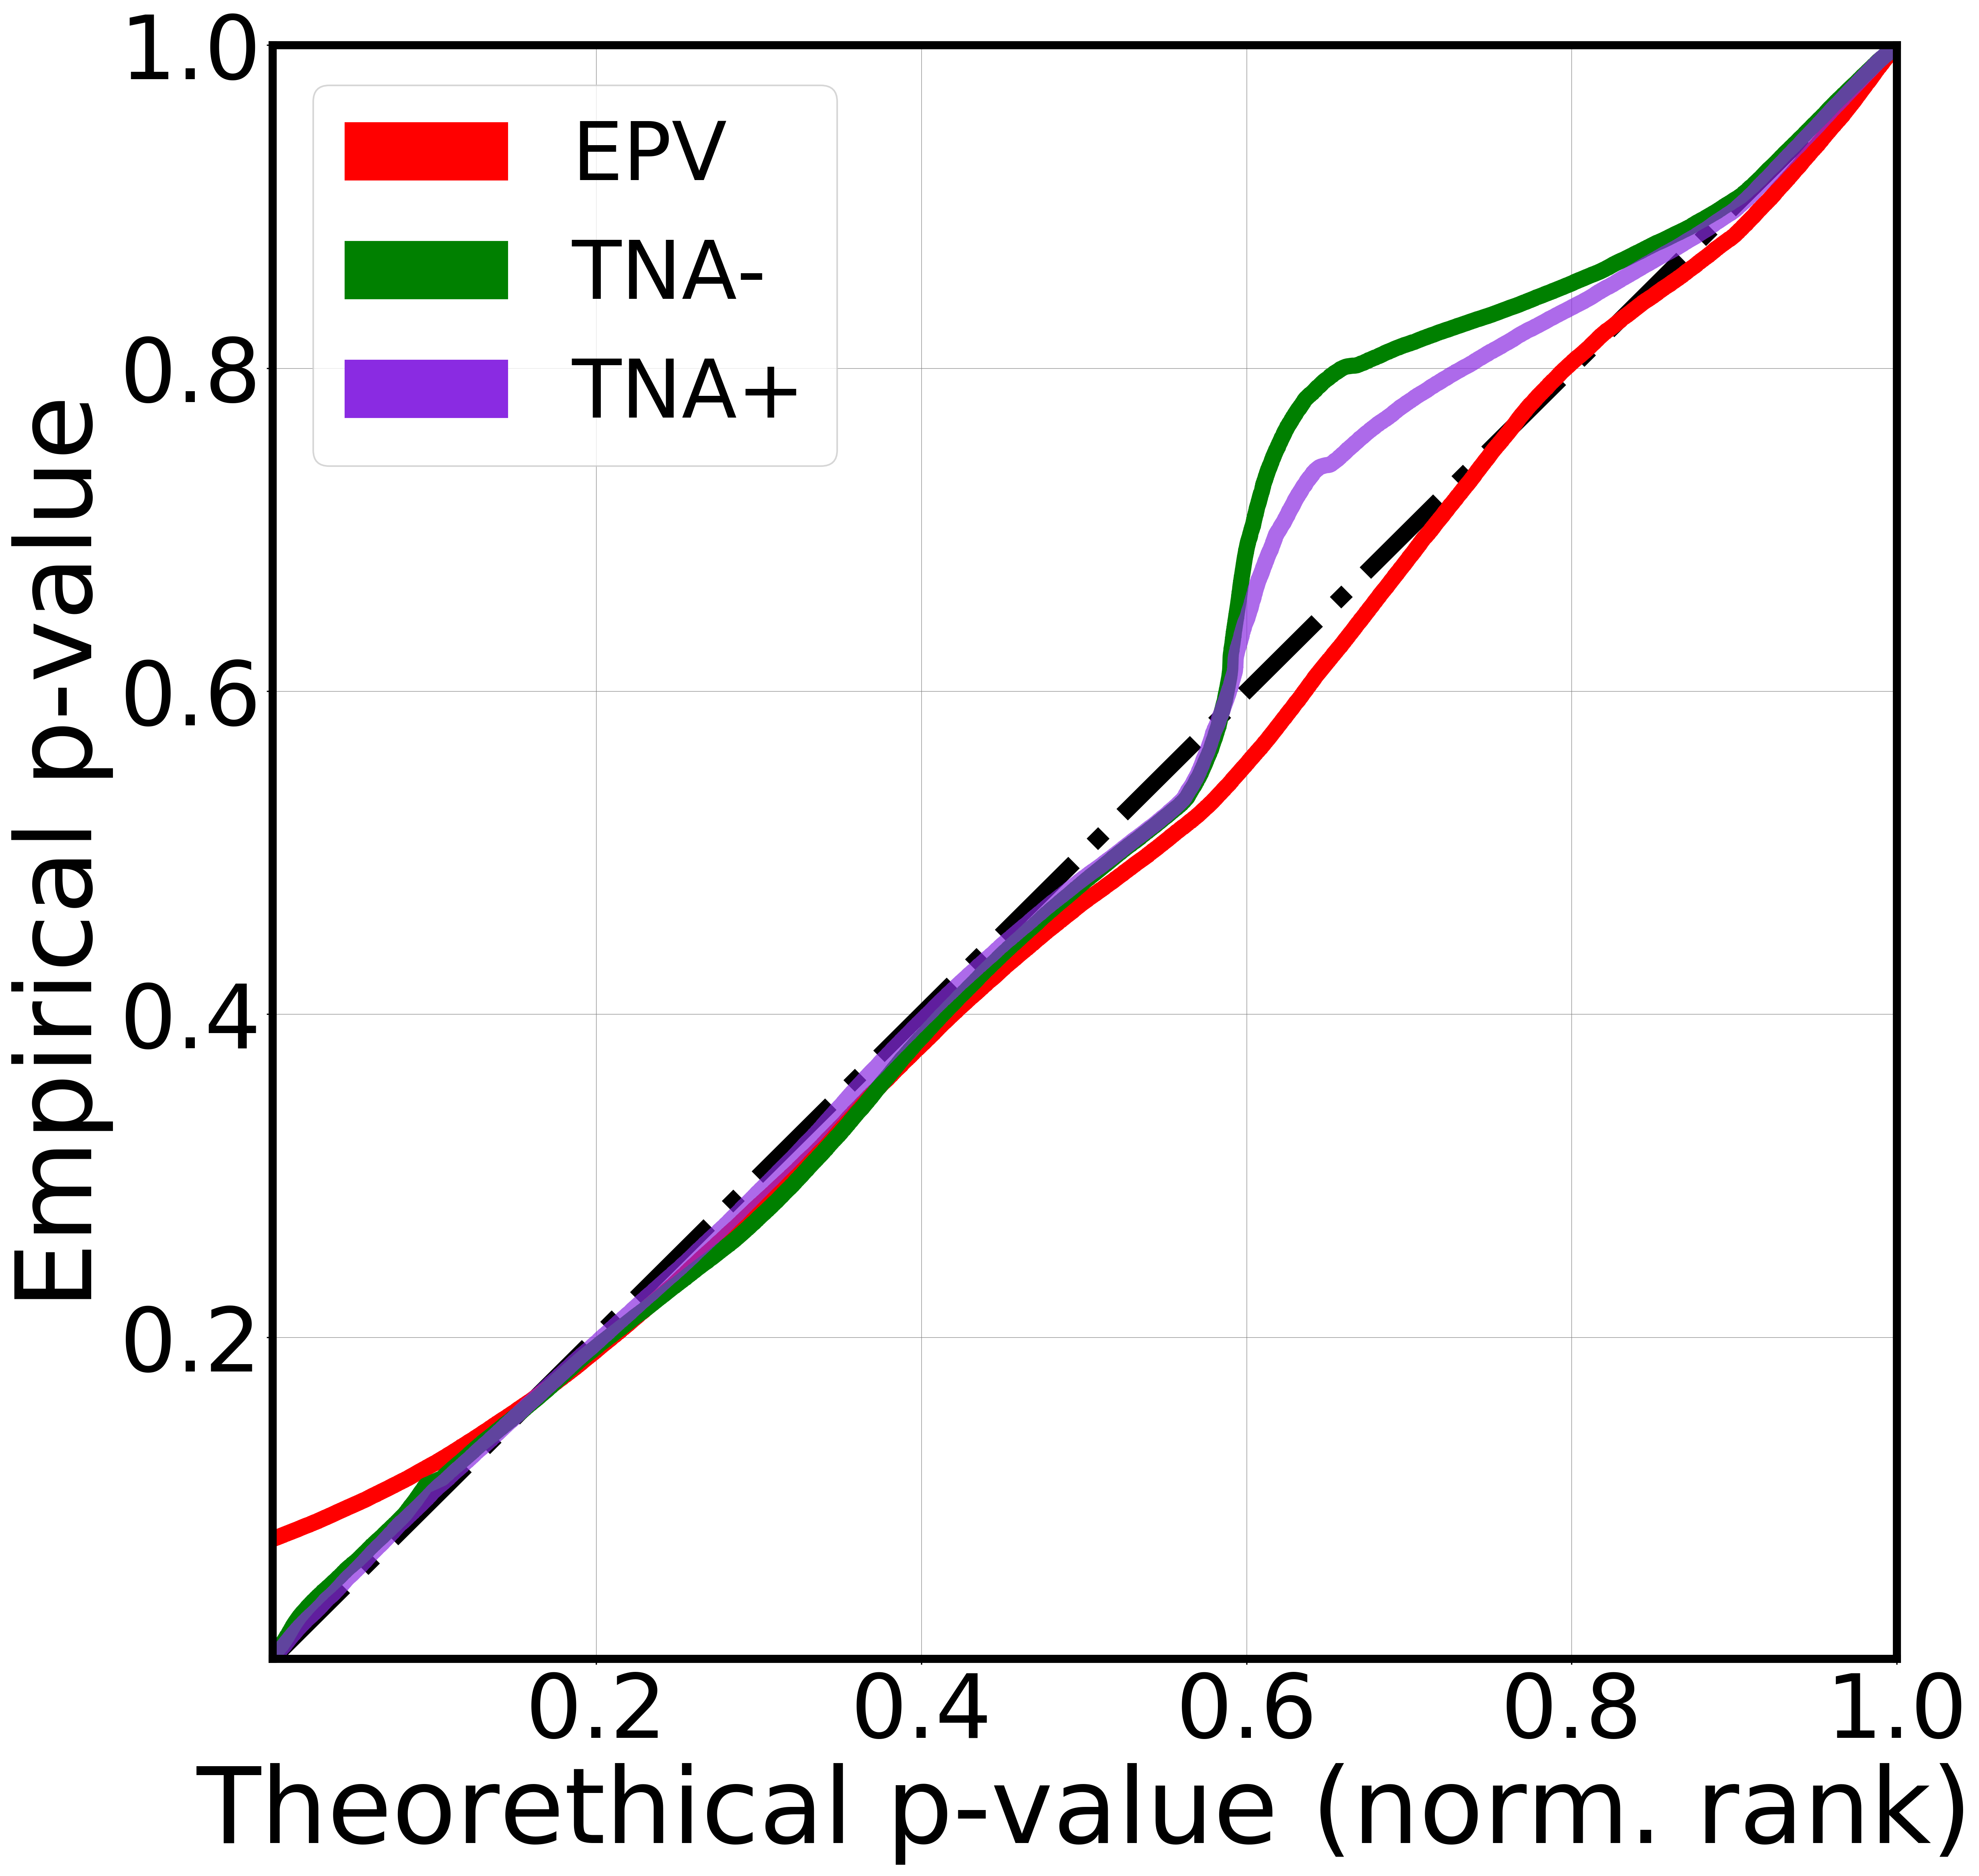
\includegraphics[width=0.225\linewidth, height=0.225\linewidth]{img/cnn_QQ_cells_segment.png} &
		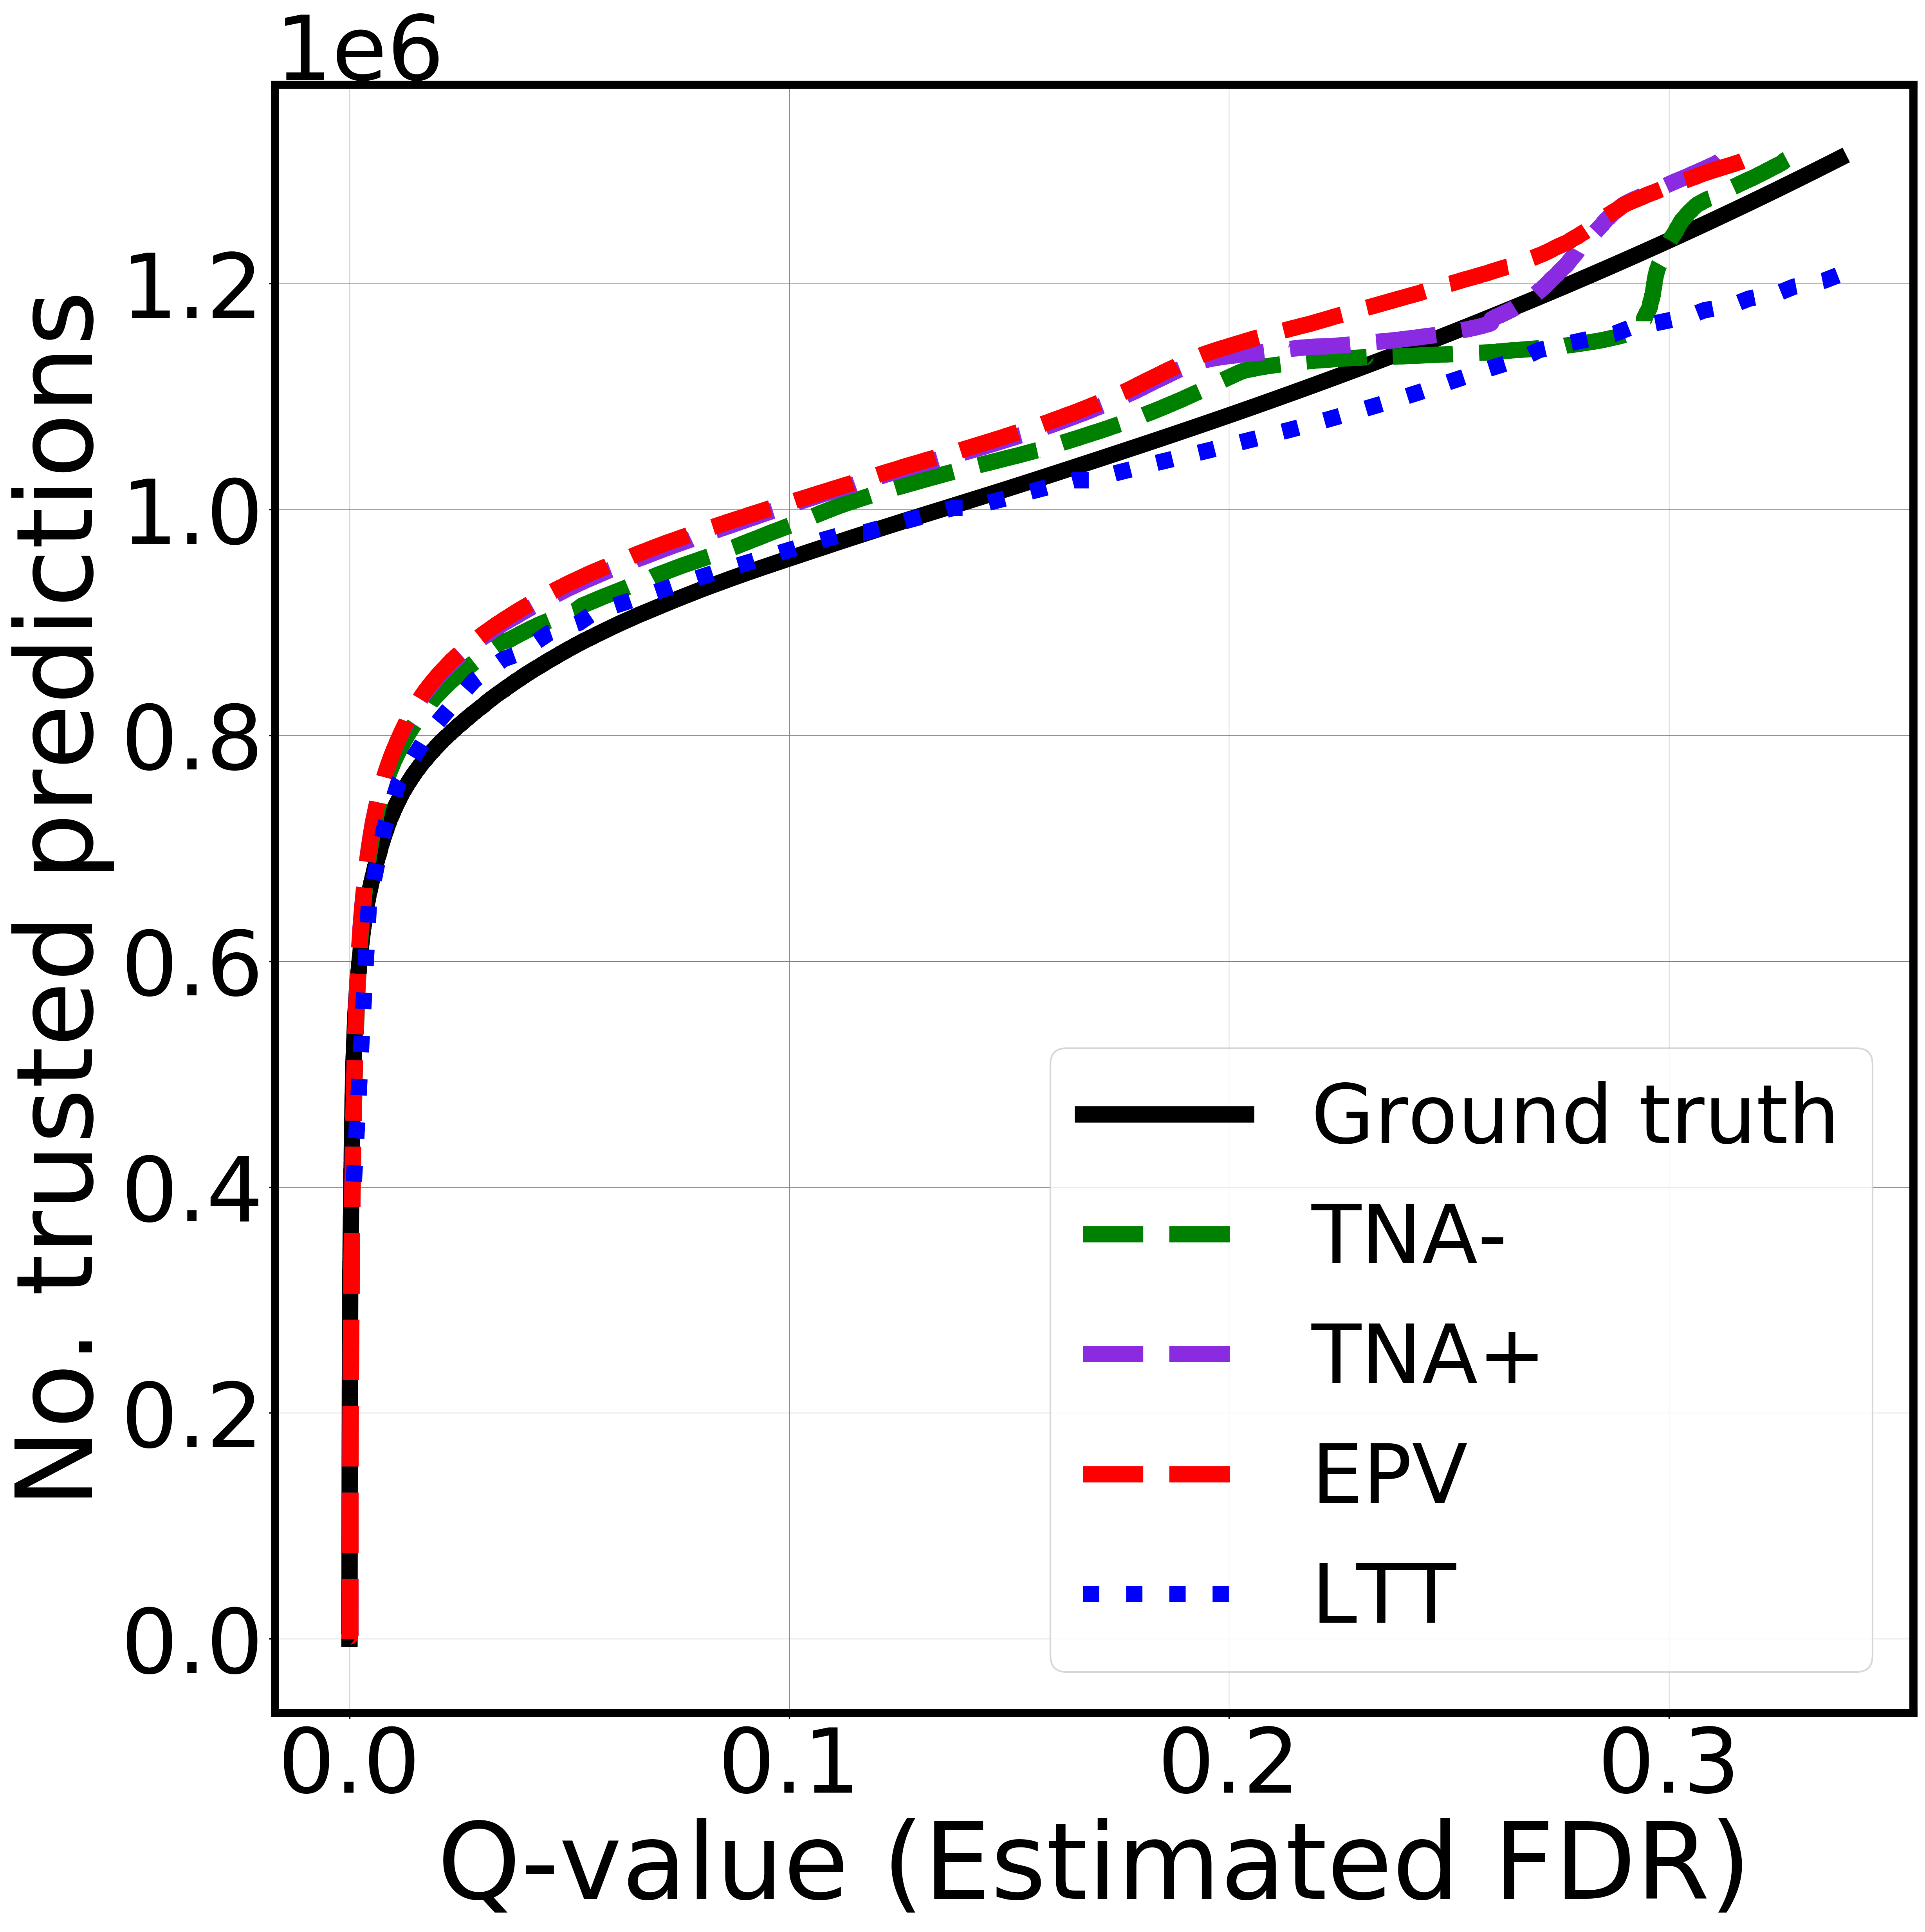
\includegraphics[width=0.225\linewidth, height=0.225\linewidth]{img/cnn_cells_segment_fdr_control.png} & 
		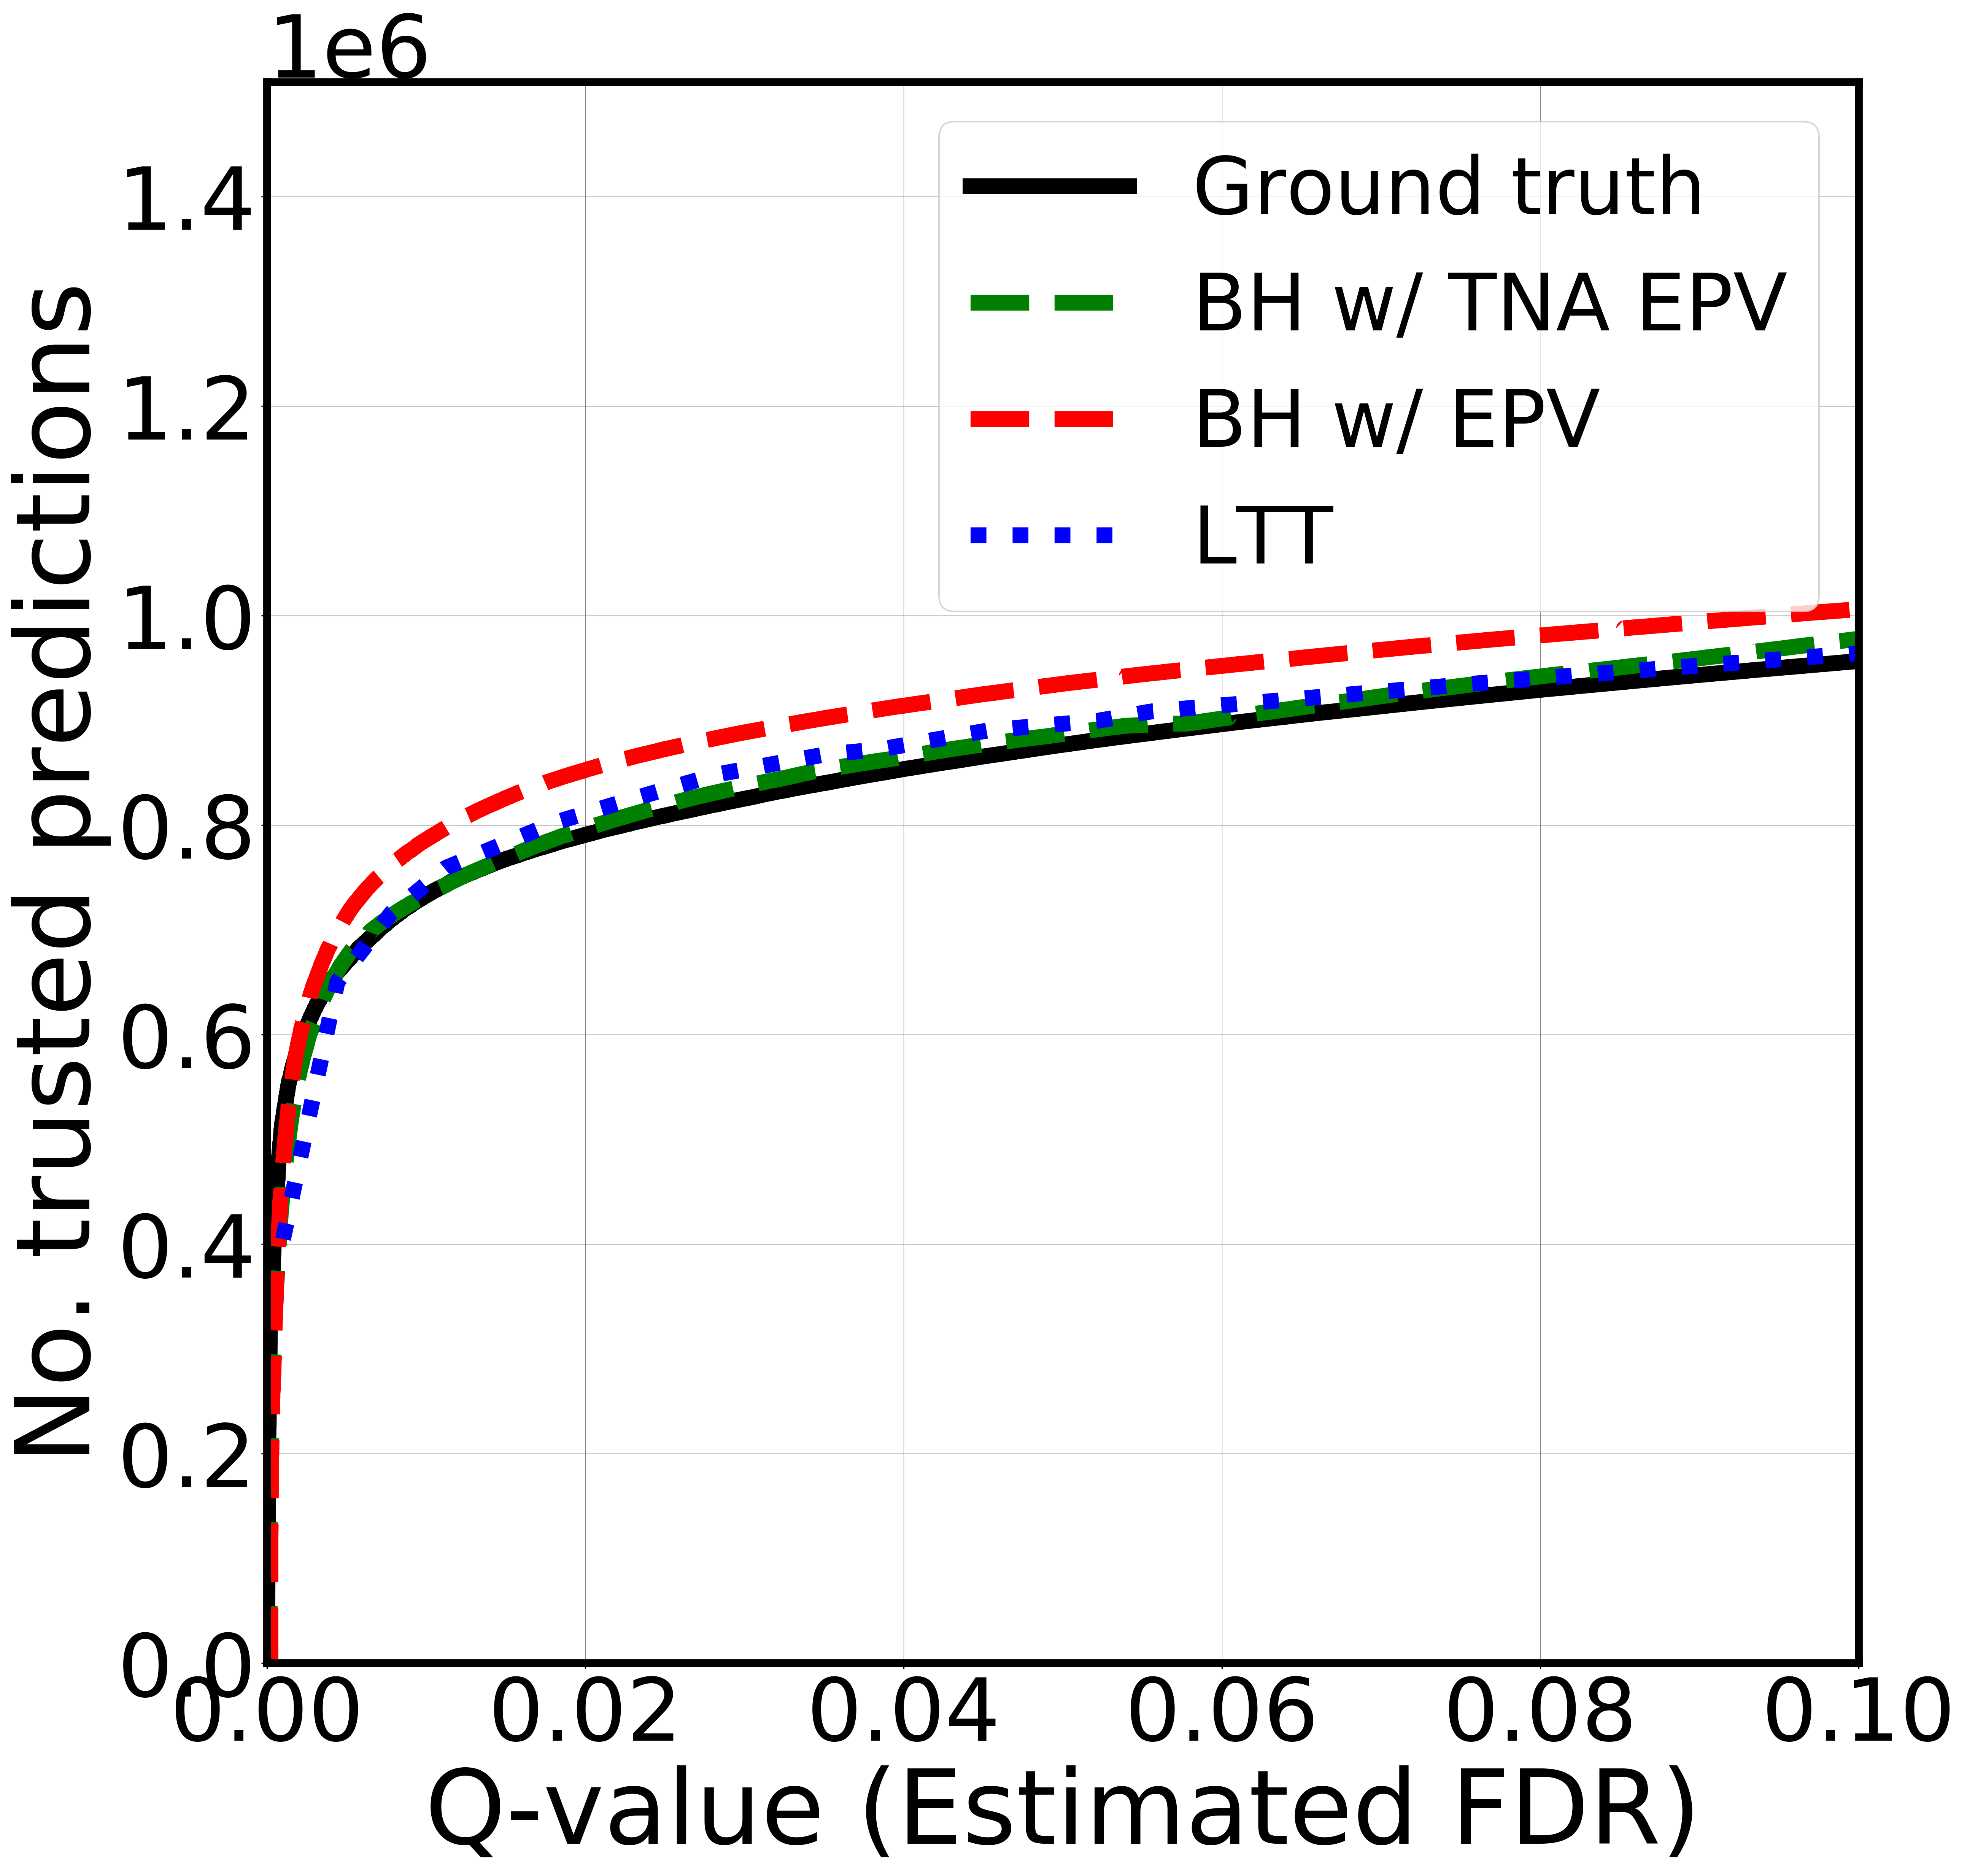
\includegraphics[width=0.225\linewidth, height=0.225\linewidth]{img/cnn_cells_segment_fdr_control_loc.png} & 
		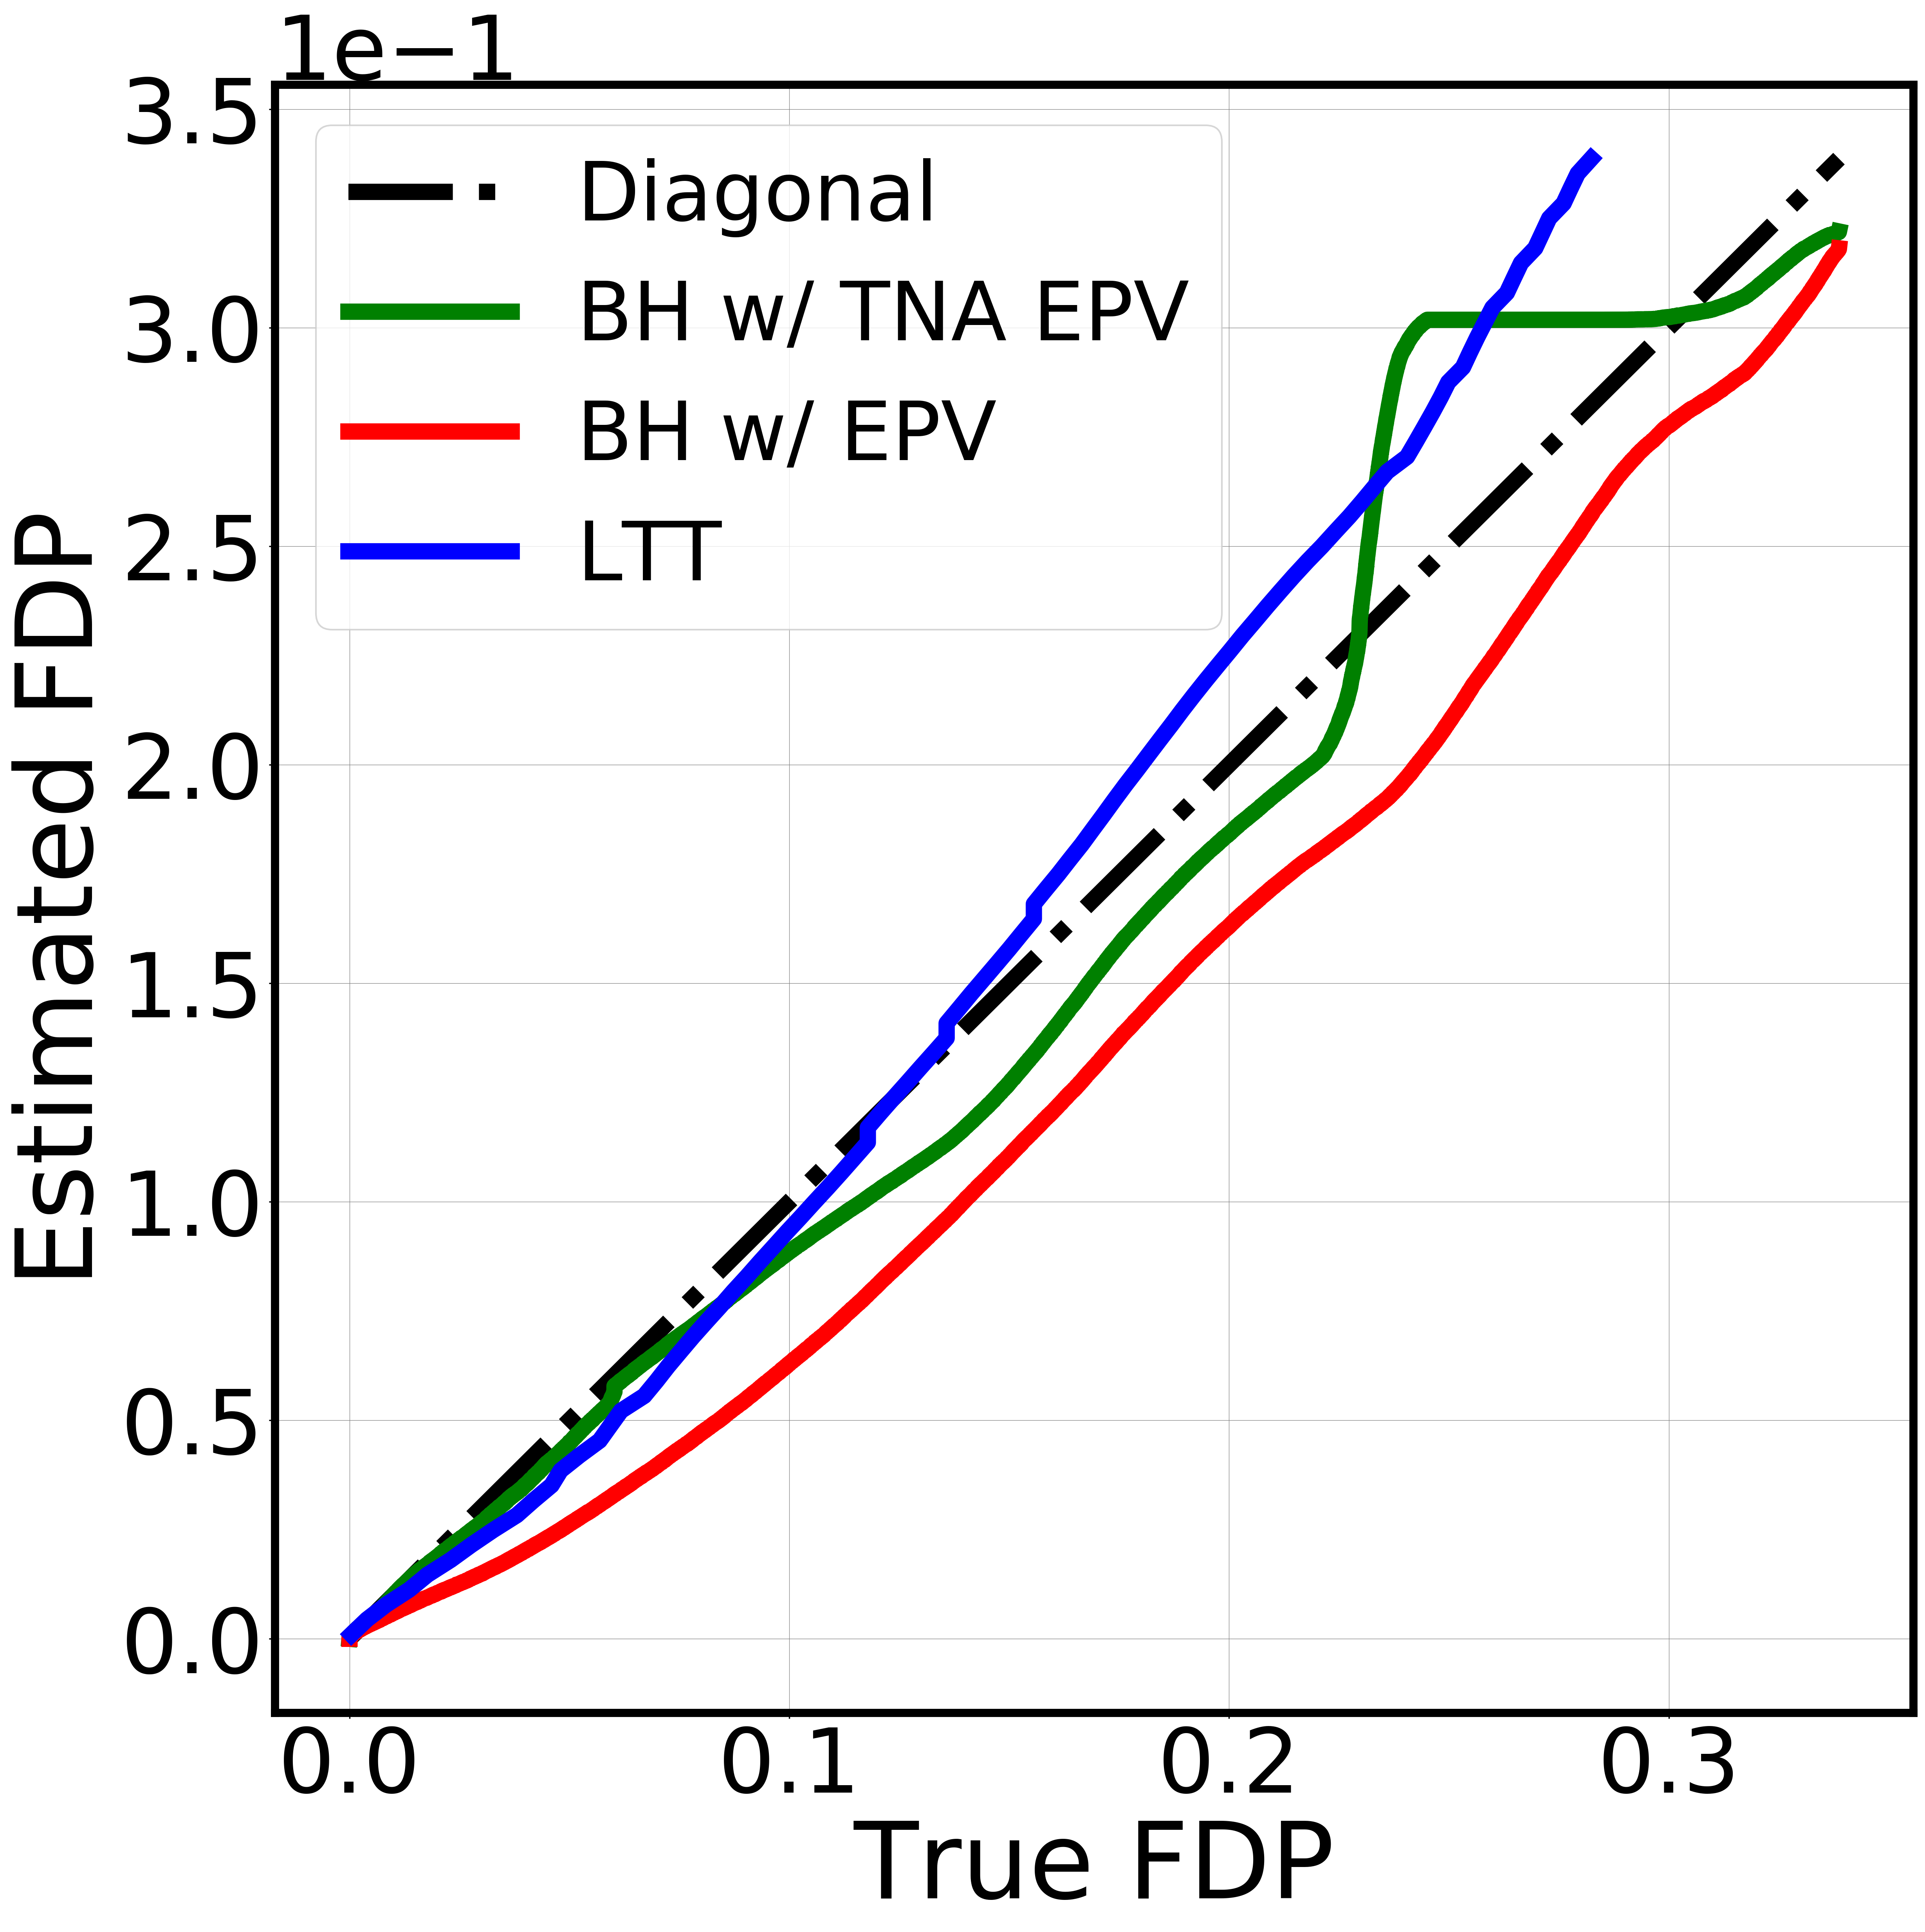
\includegraphics[width=0.225\linewidth, height=0.225\linewidth]{img/cnn_FDPscat_cells_segment.png}\\	
		\multicolumn{4}{l}{\bf (ii) TissueNet with single image:}\\		
		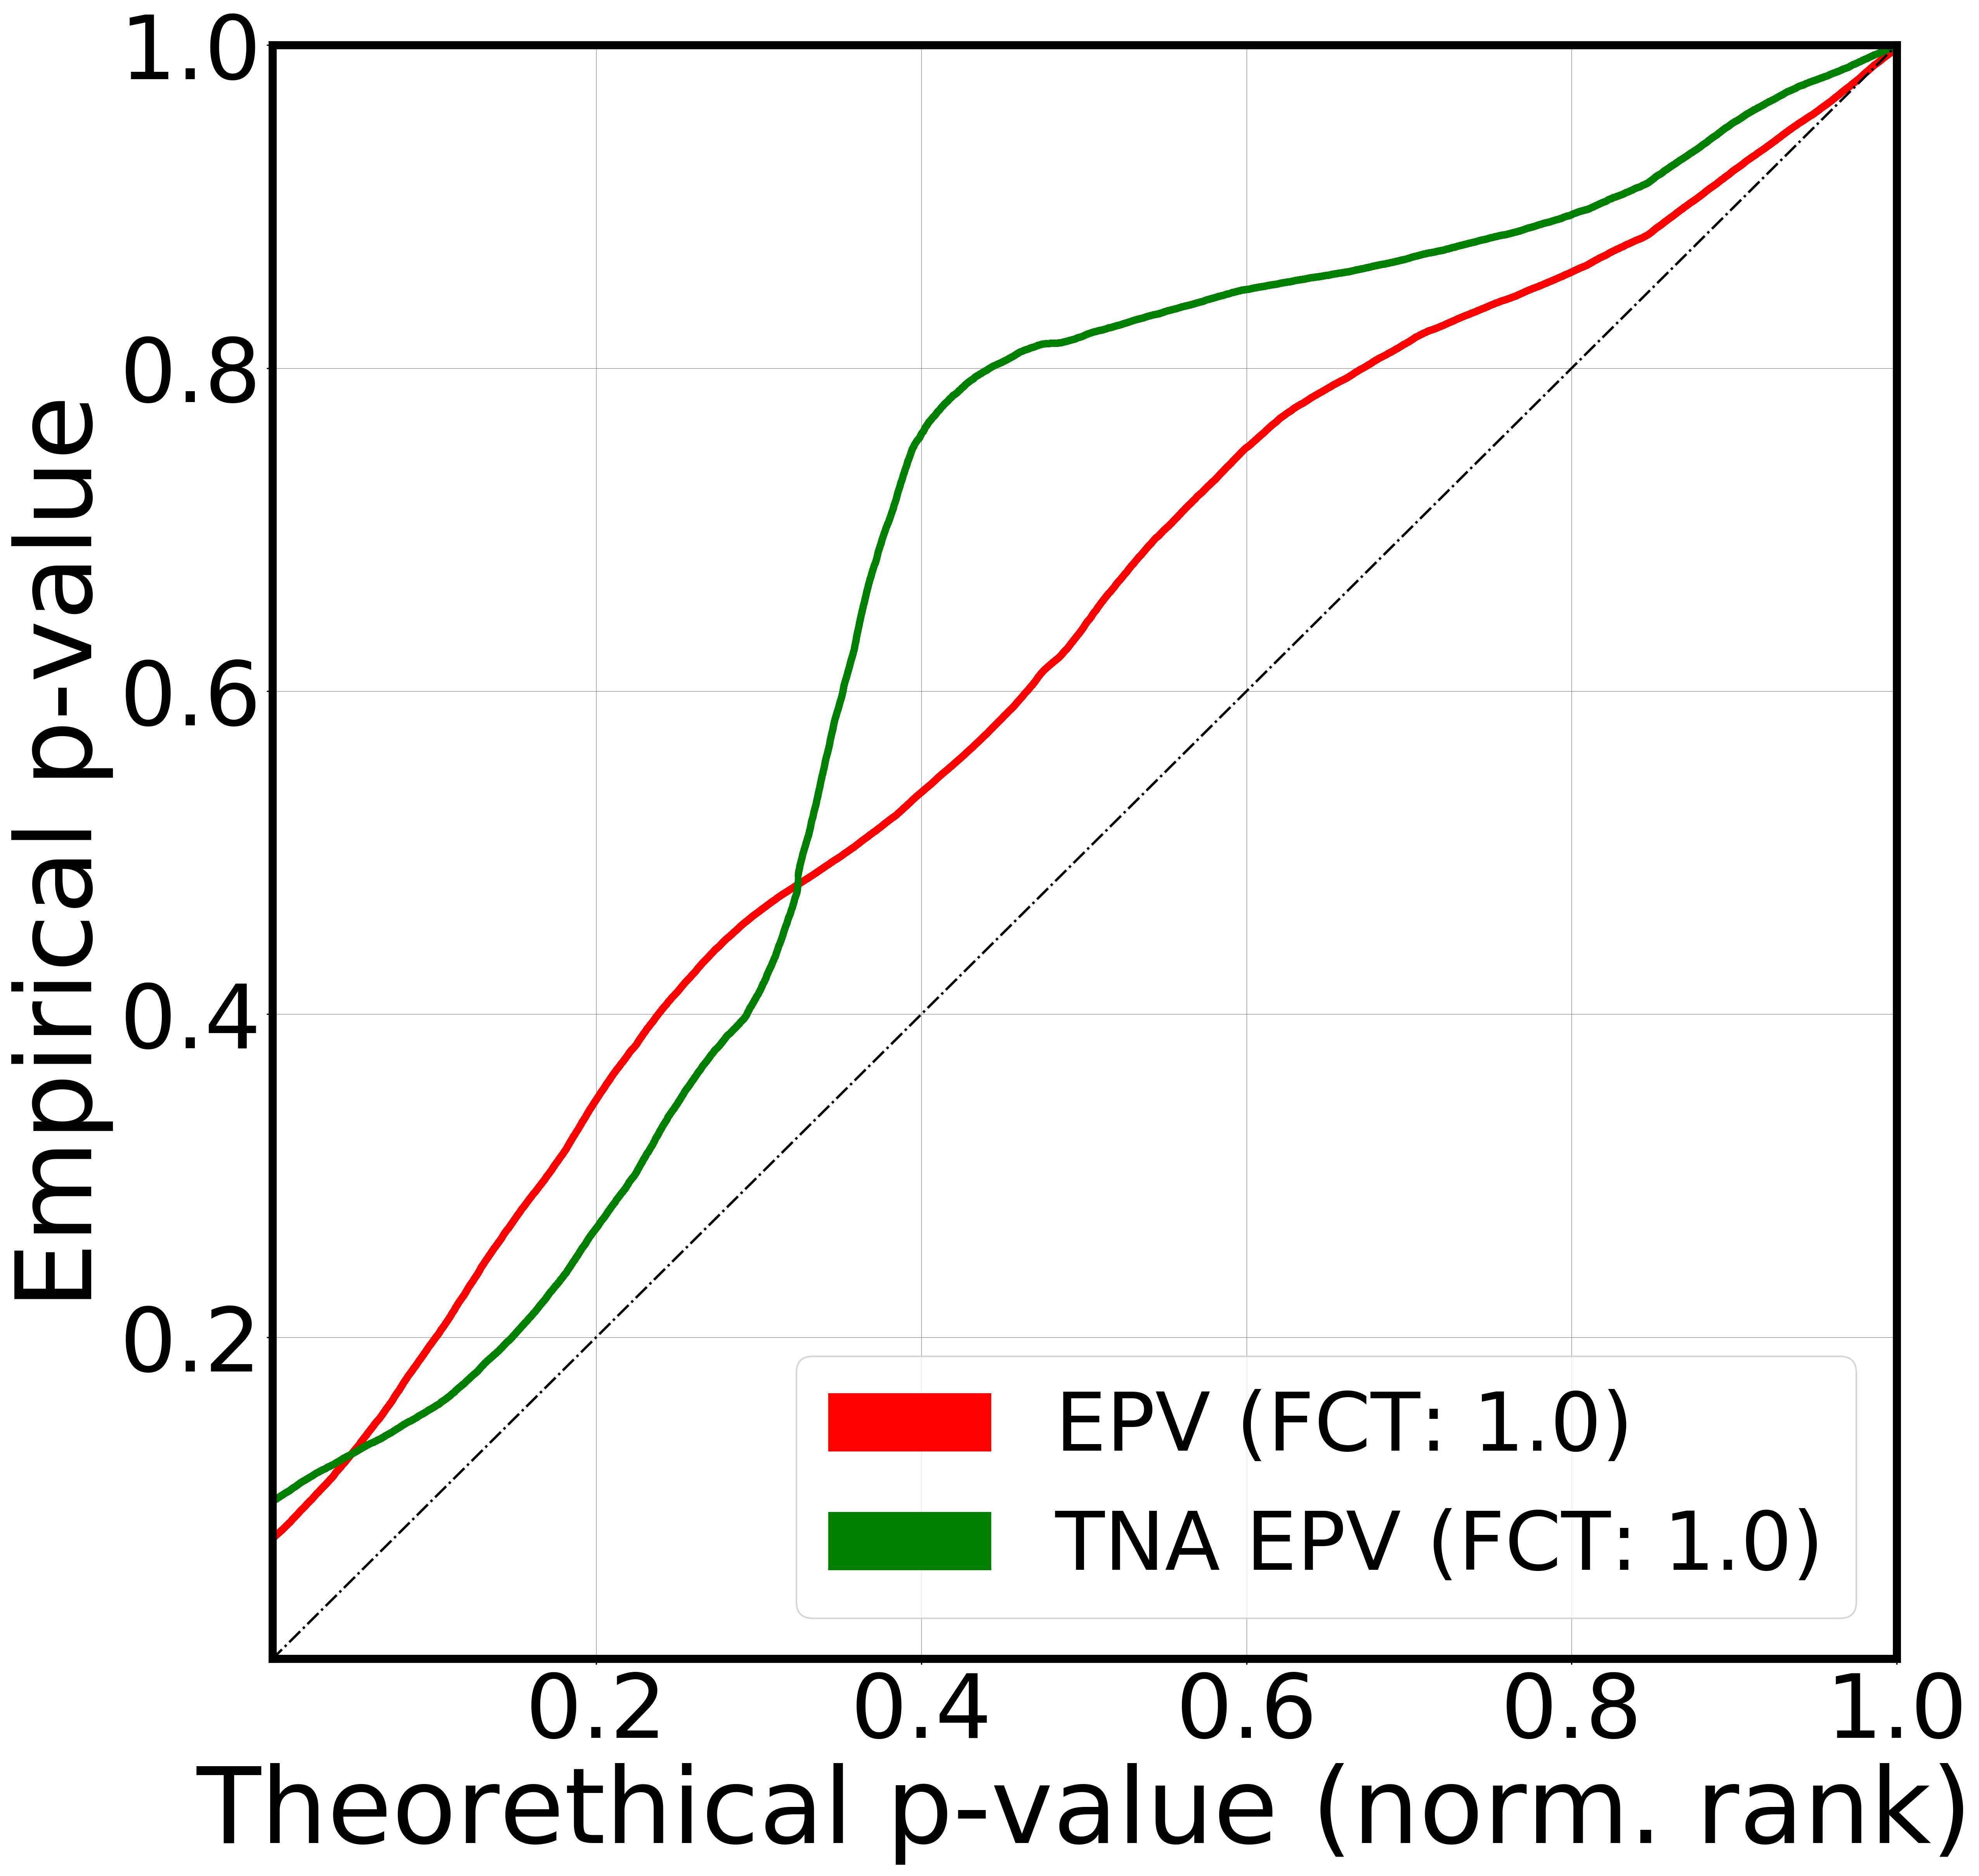
\includegraphics[width=0.225\linewidth, height=0.225\linewidth]{img/cnn_QQ_cells_balanced.png} &
		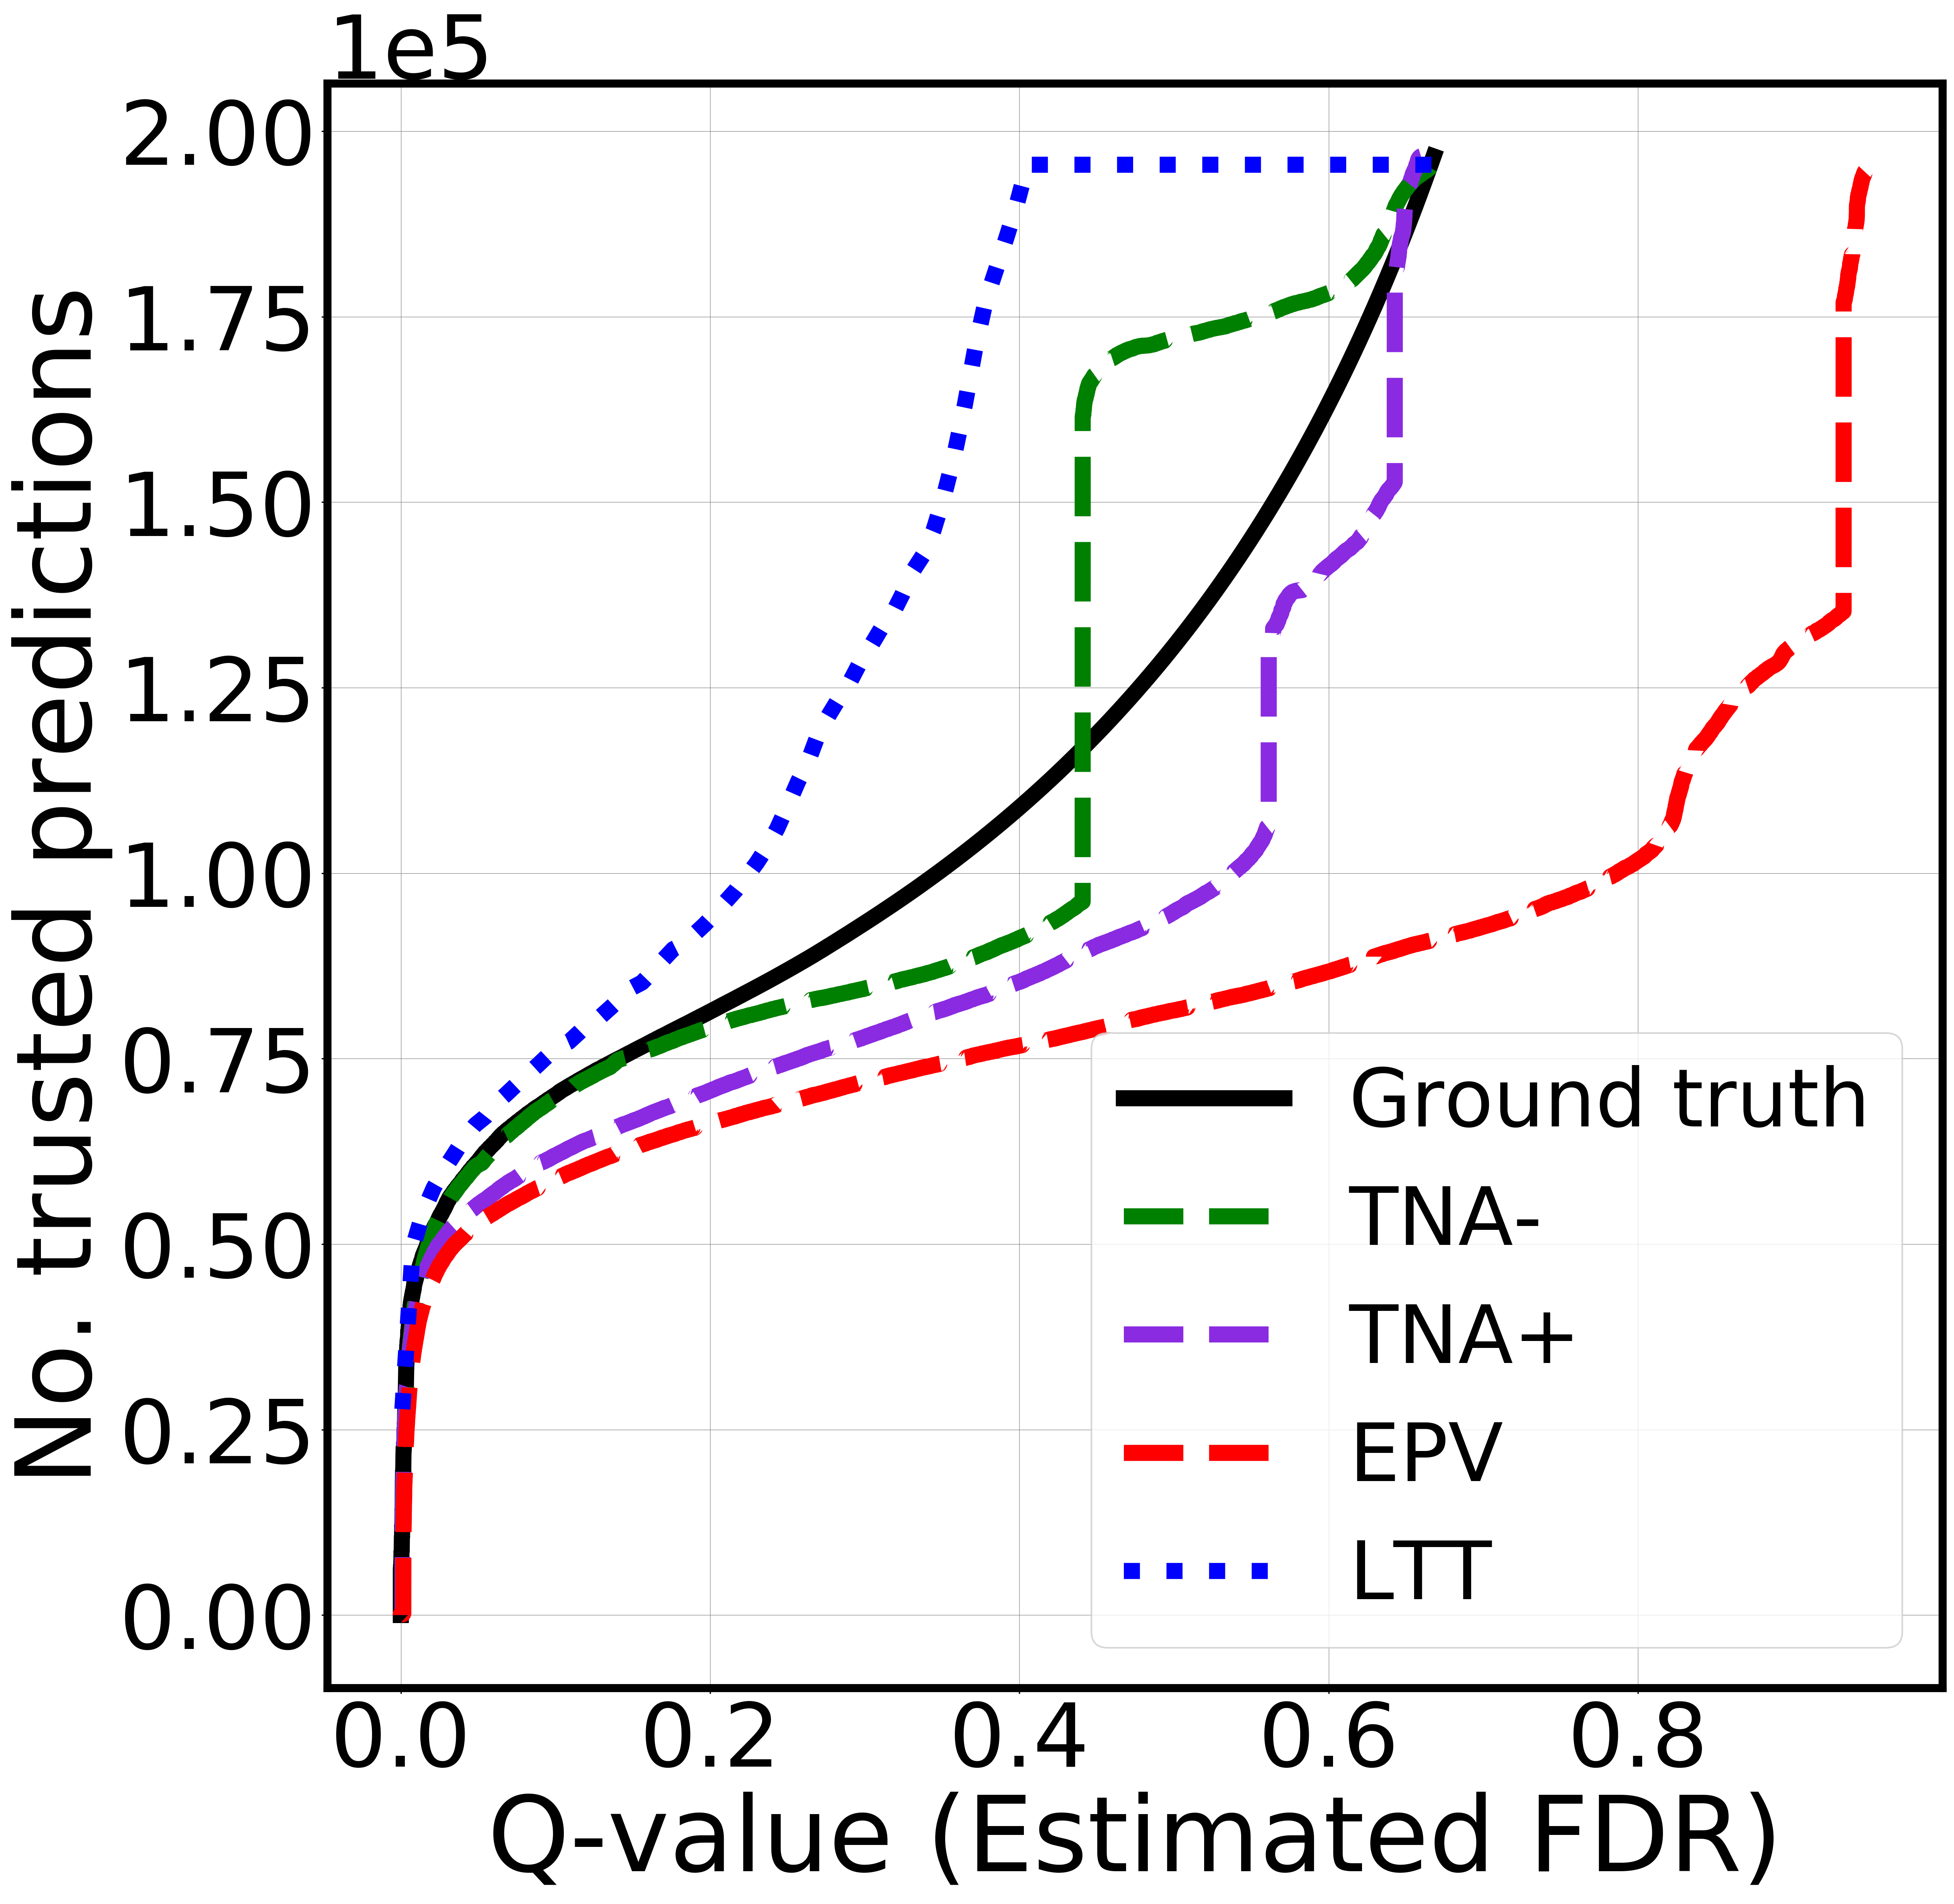
\includegraphics[width=0.225\linewidth, height=0.225\linewidth]{img/cnn_cells_balanced_fdr_control.png} & 
		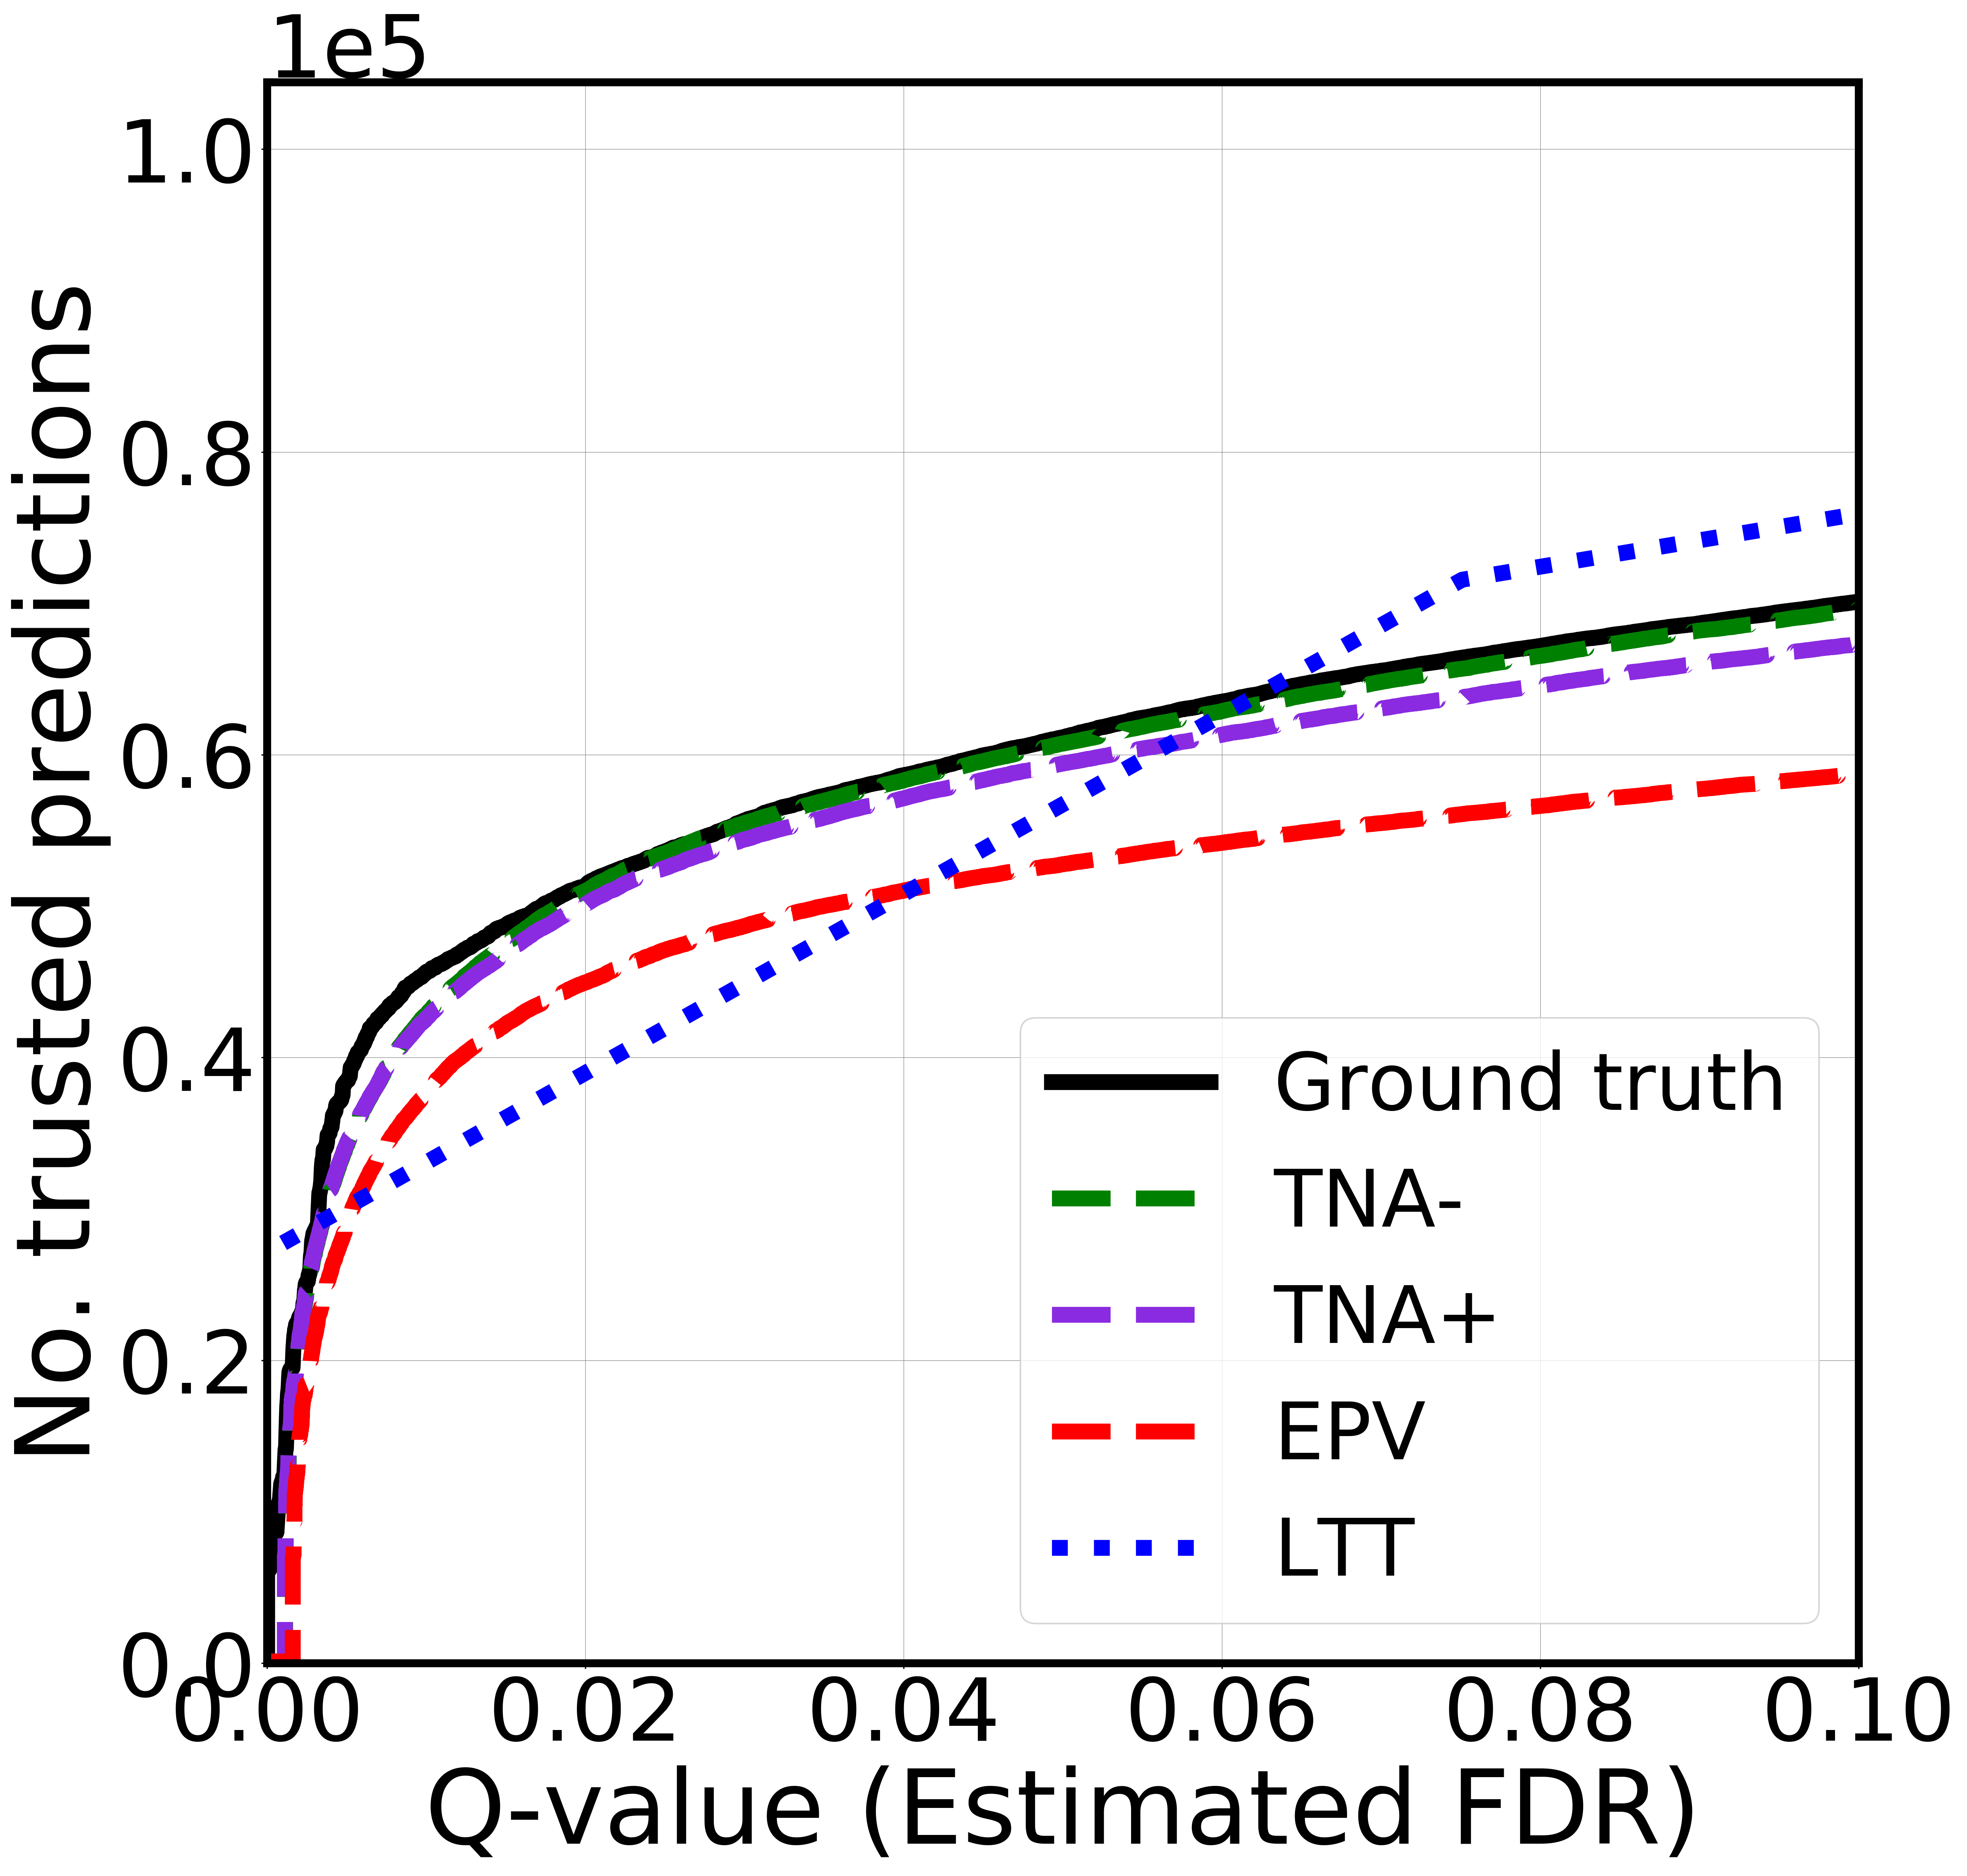
\includegraphics[width=0.225\linewidth, height=0.225\linewidth]{img/cnn_cells_balanced_fdr_control_loc.png} & 
		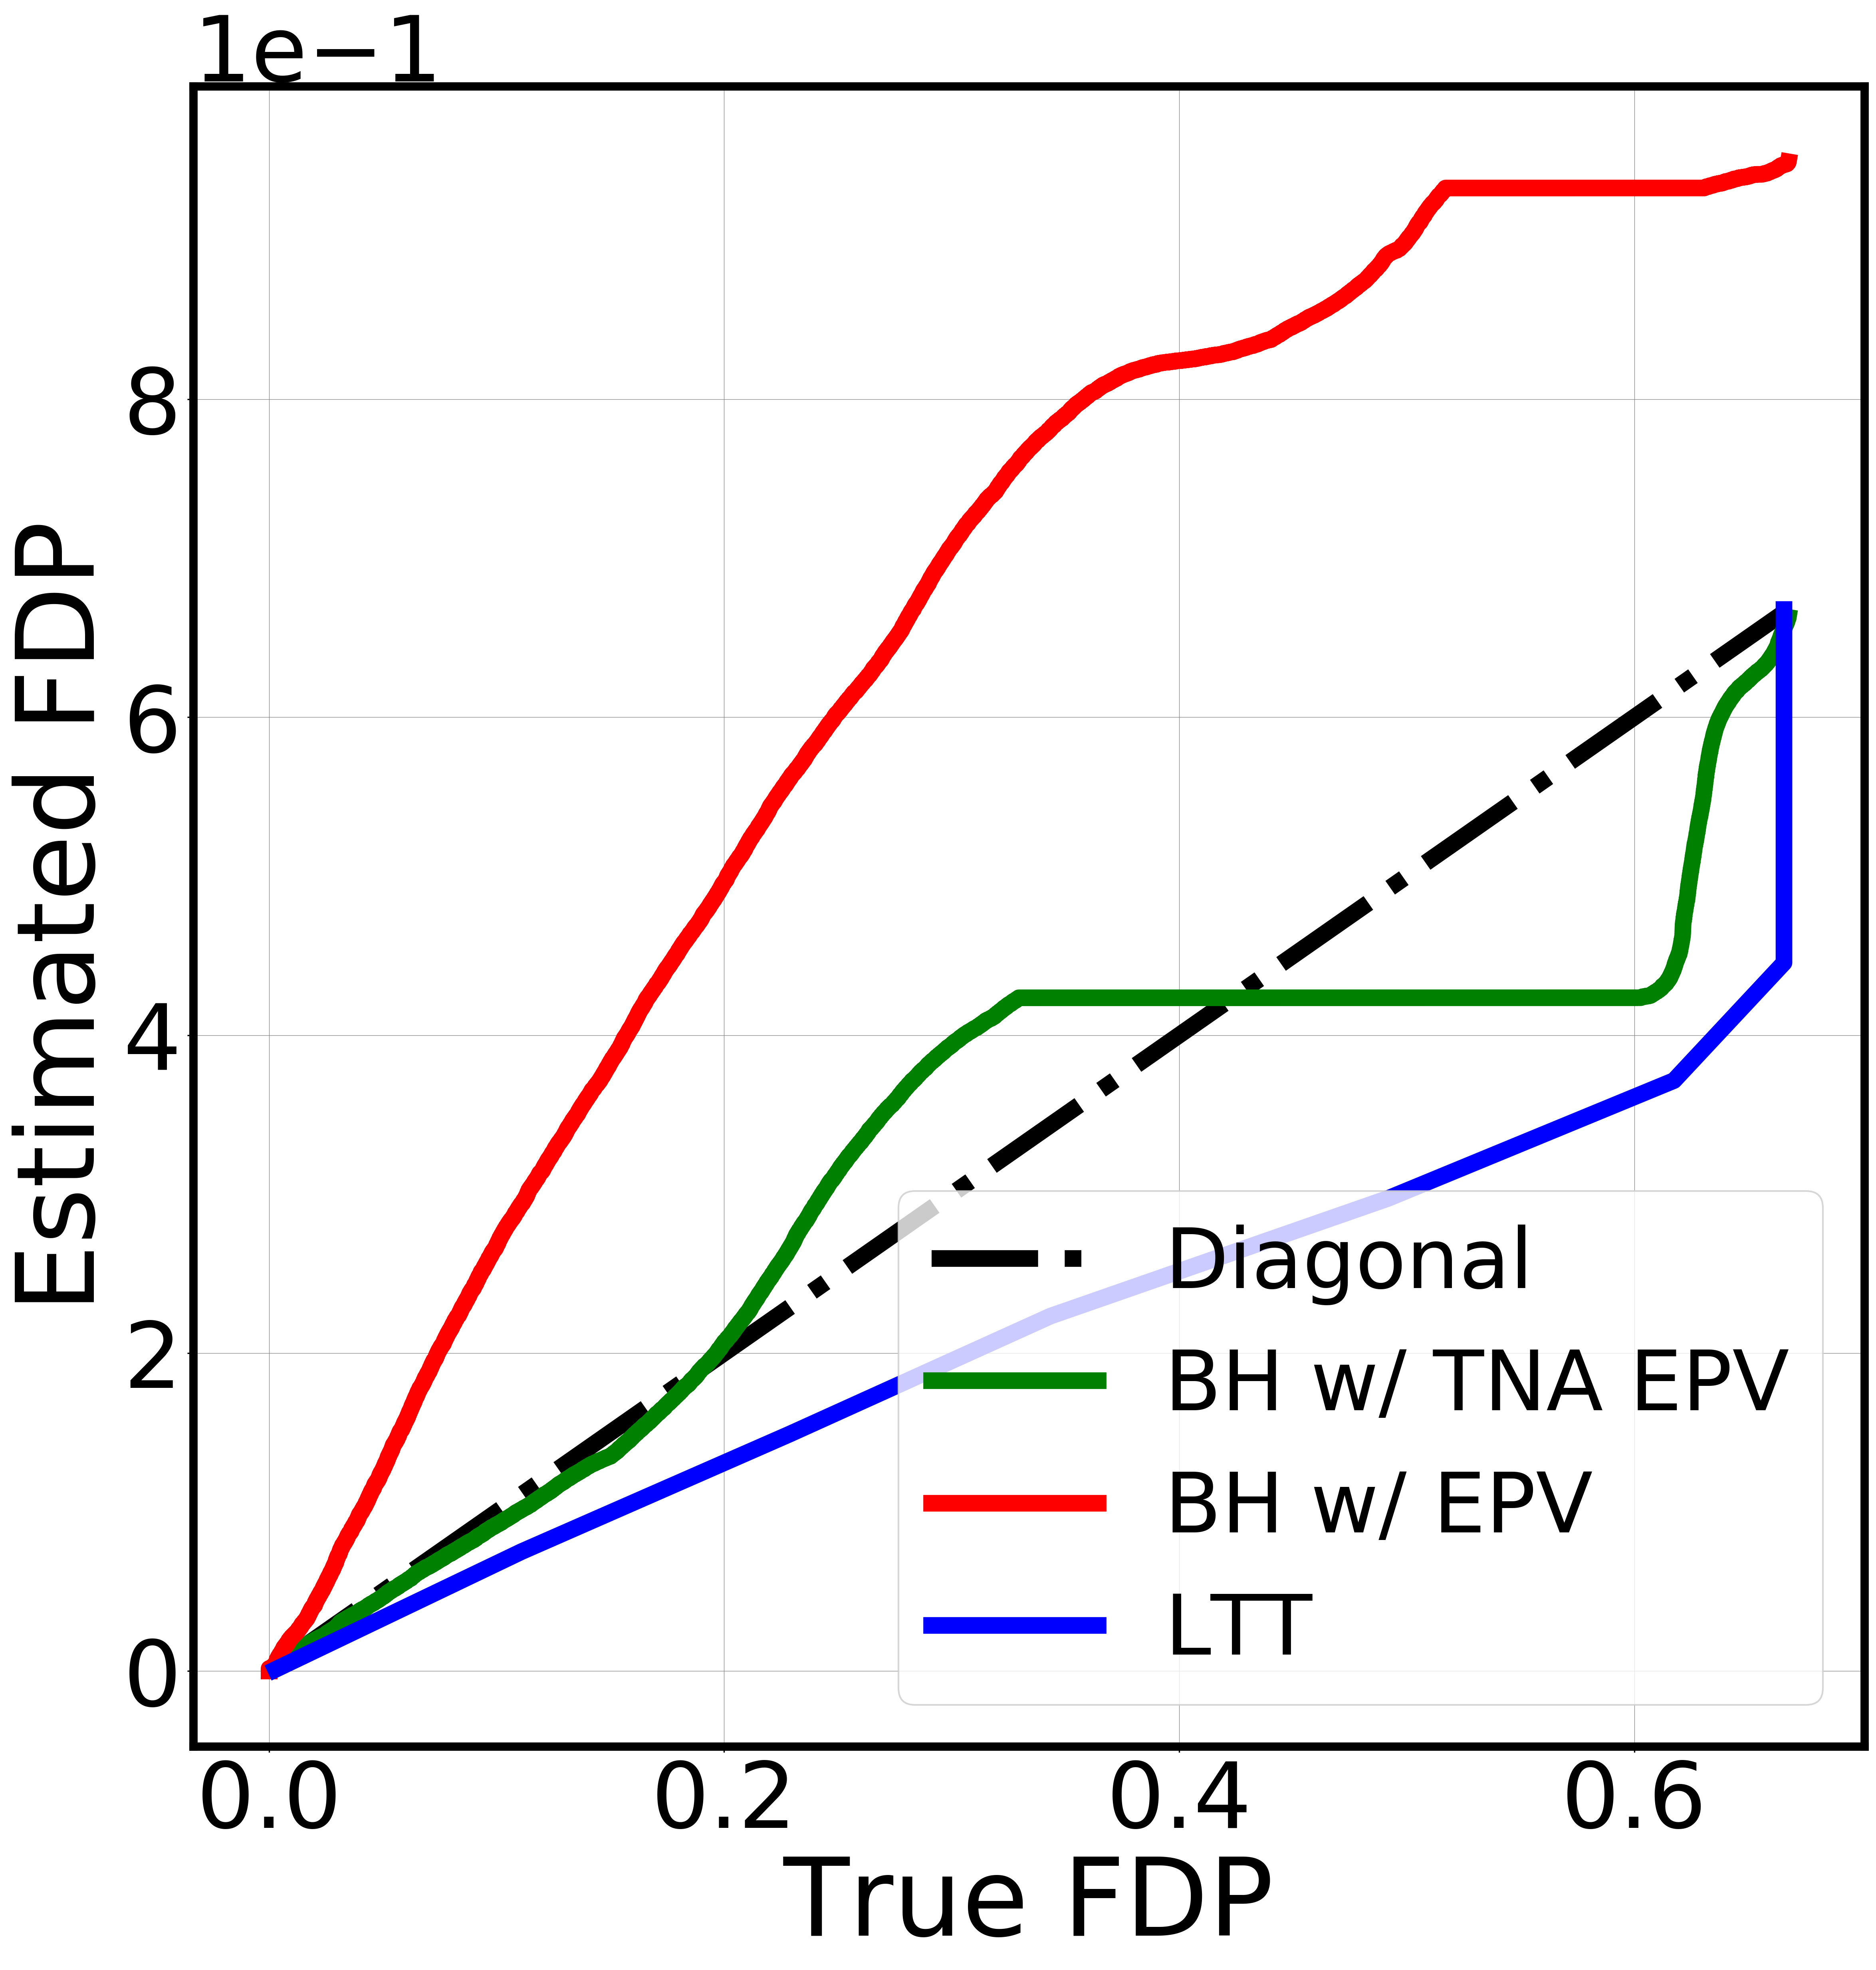
\includegraphics[width=0.225\linewidth, height=0.225\linewidth]{img/cnn_FDPscat_cells_balanced.png}\\			
		\multicolumn{4}{l}{\bf (iii) Standard BCSS dataset:}\\		
		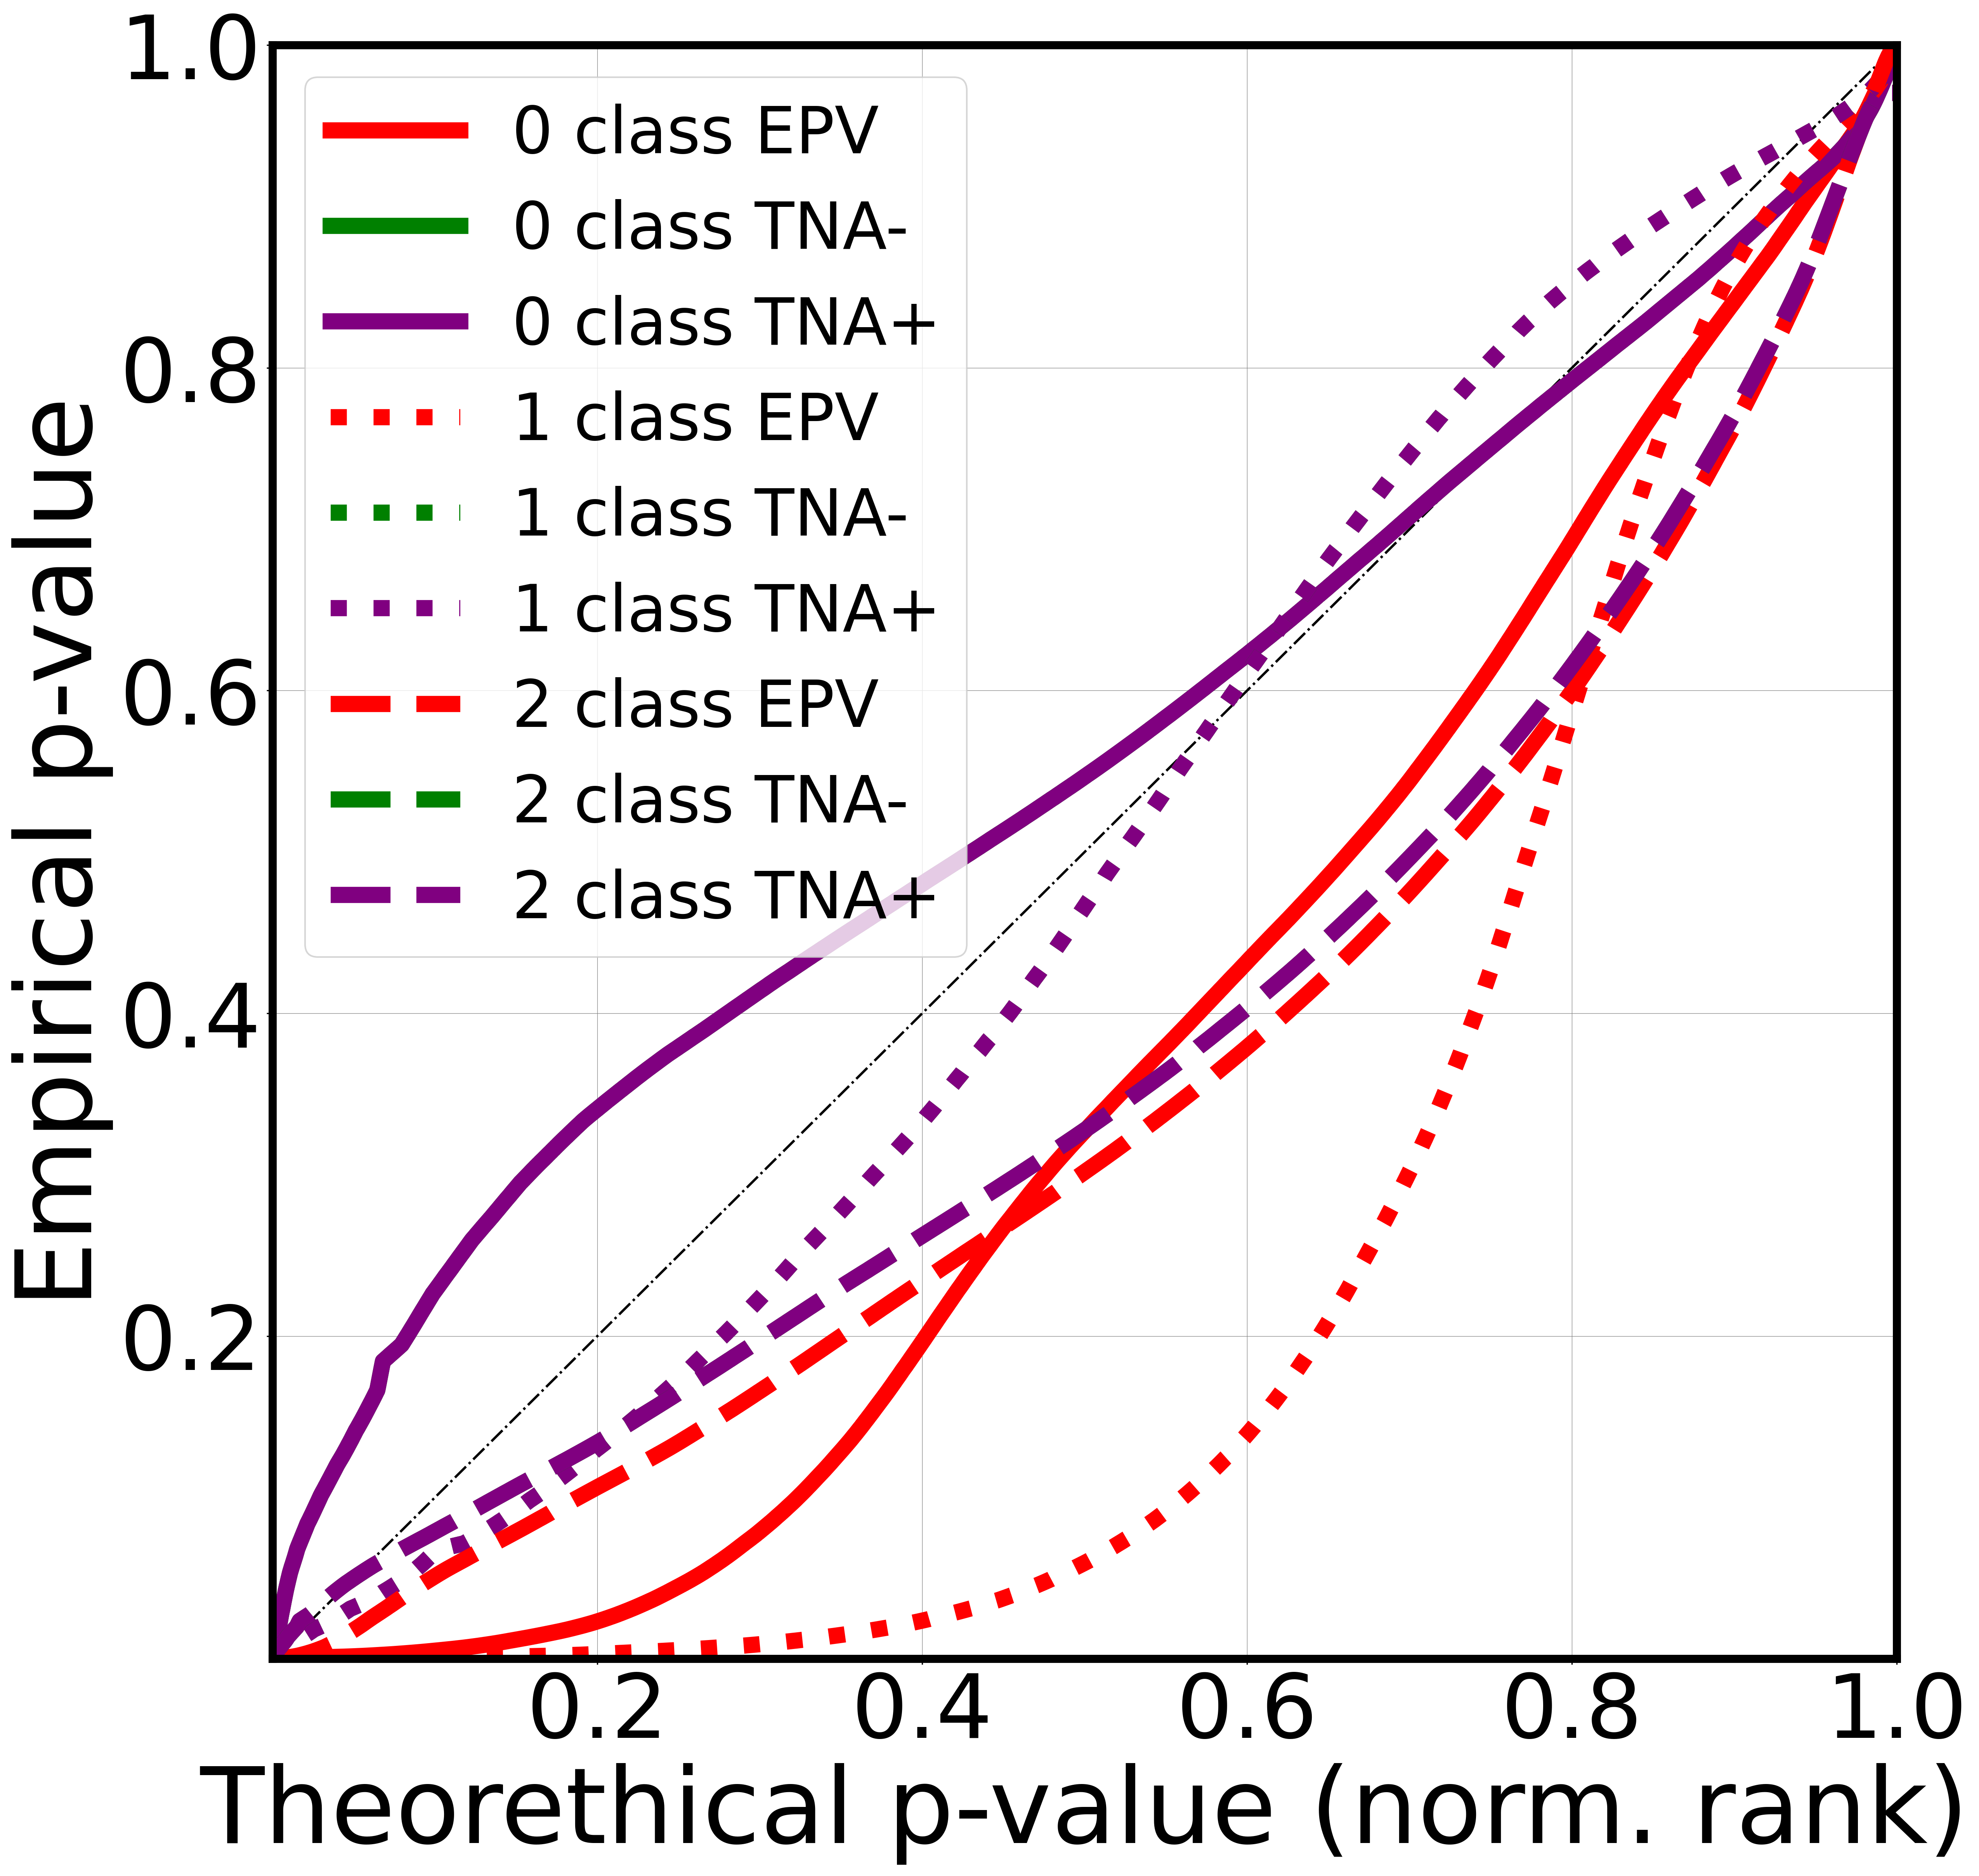
\includegraphics[width=0.225\linewidth, height=0.225\linewidth]{img/cnn_QQ_bcss.png} &
		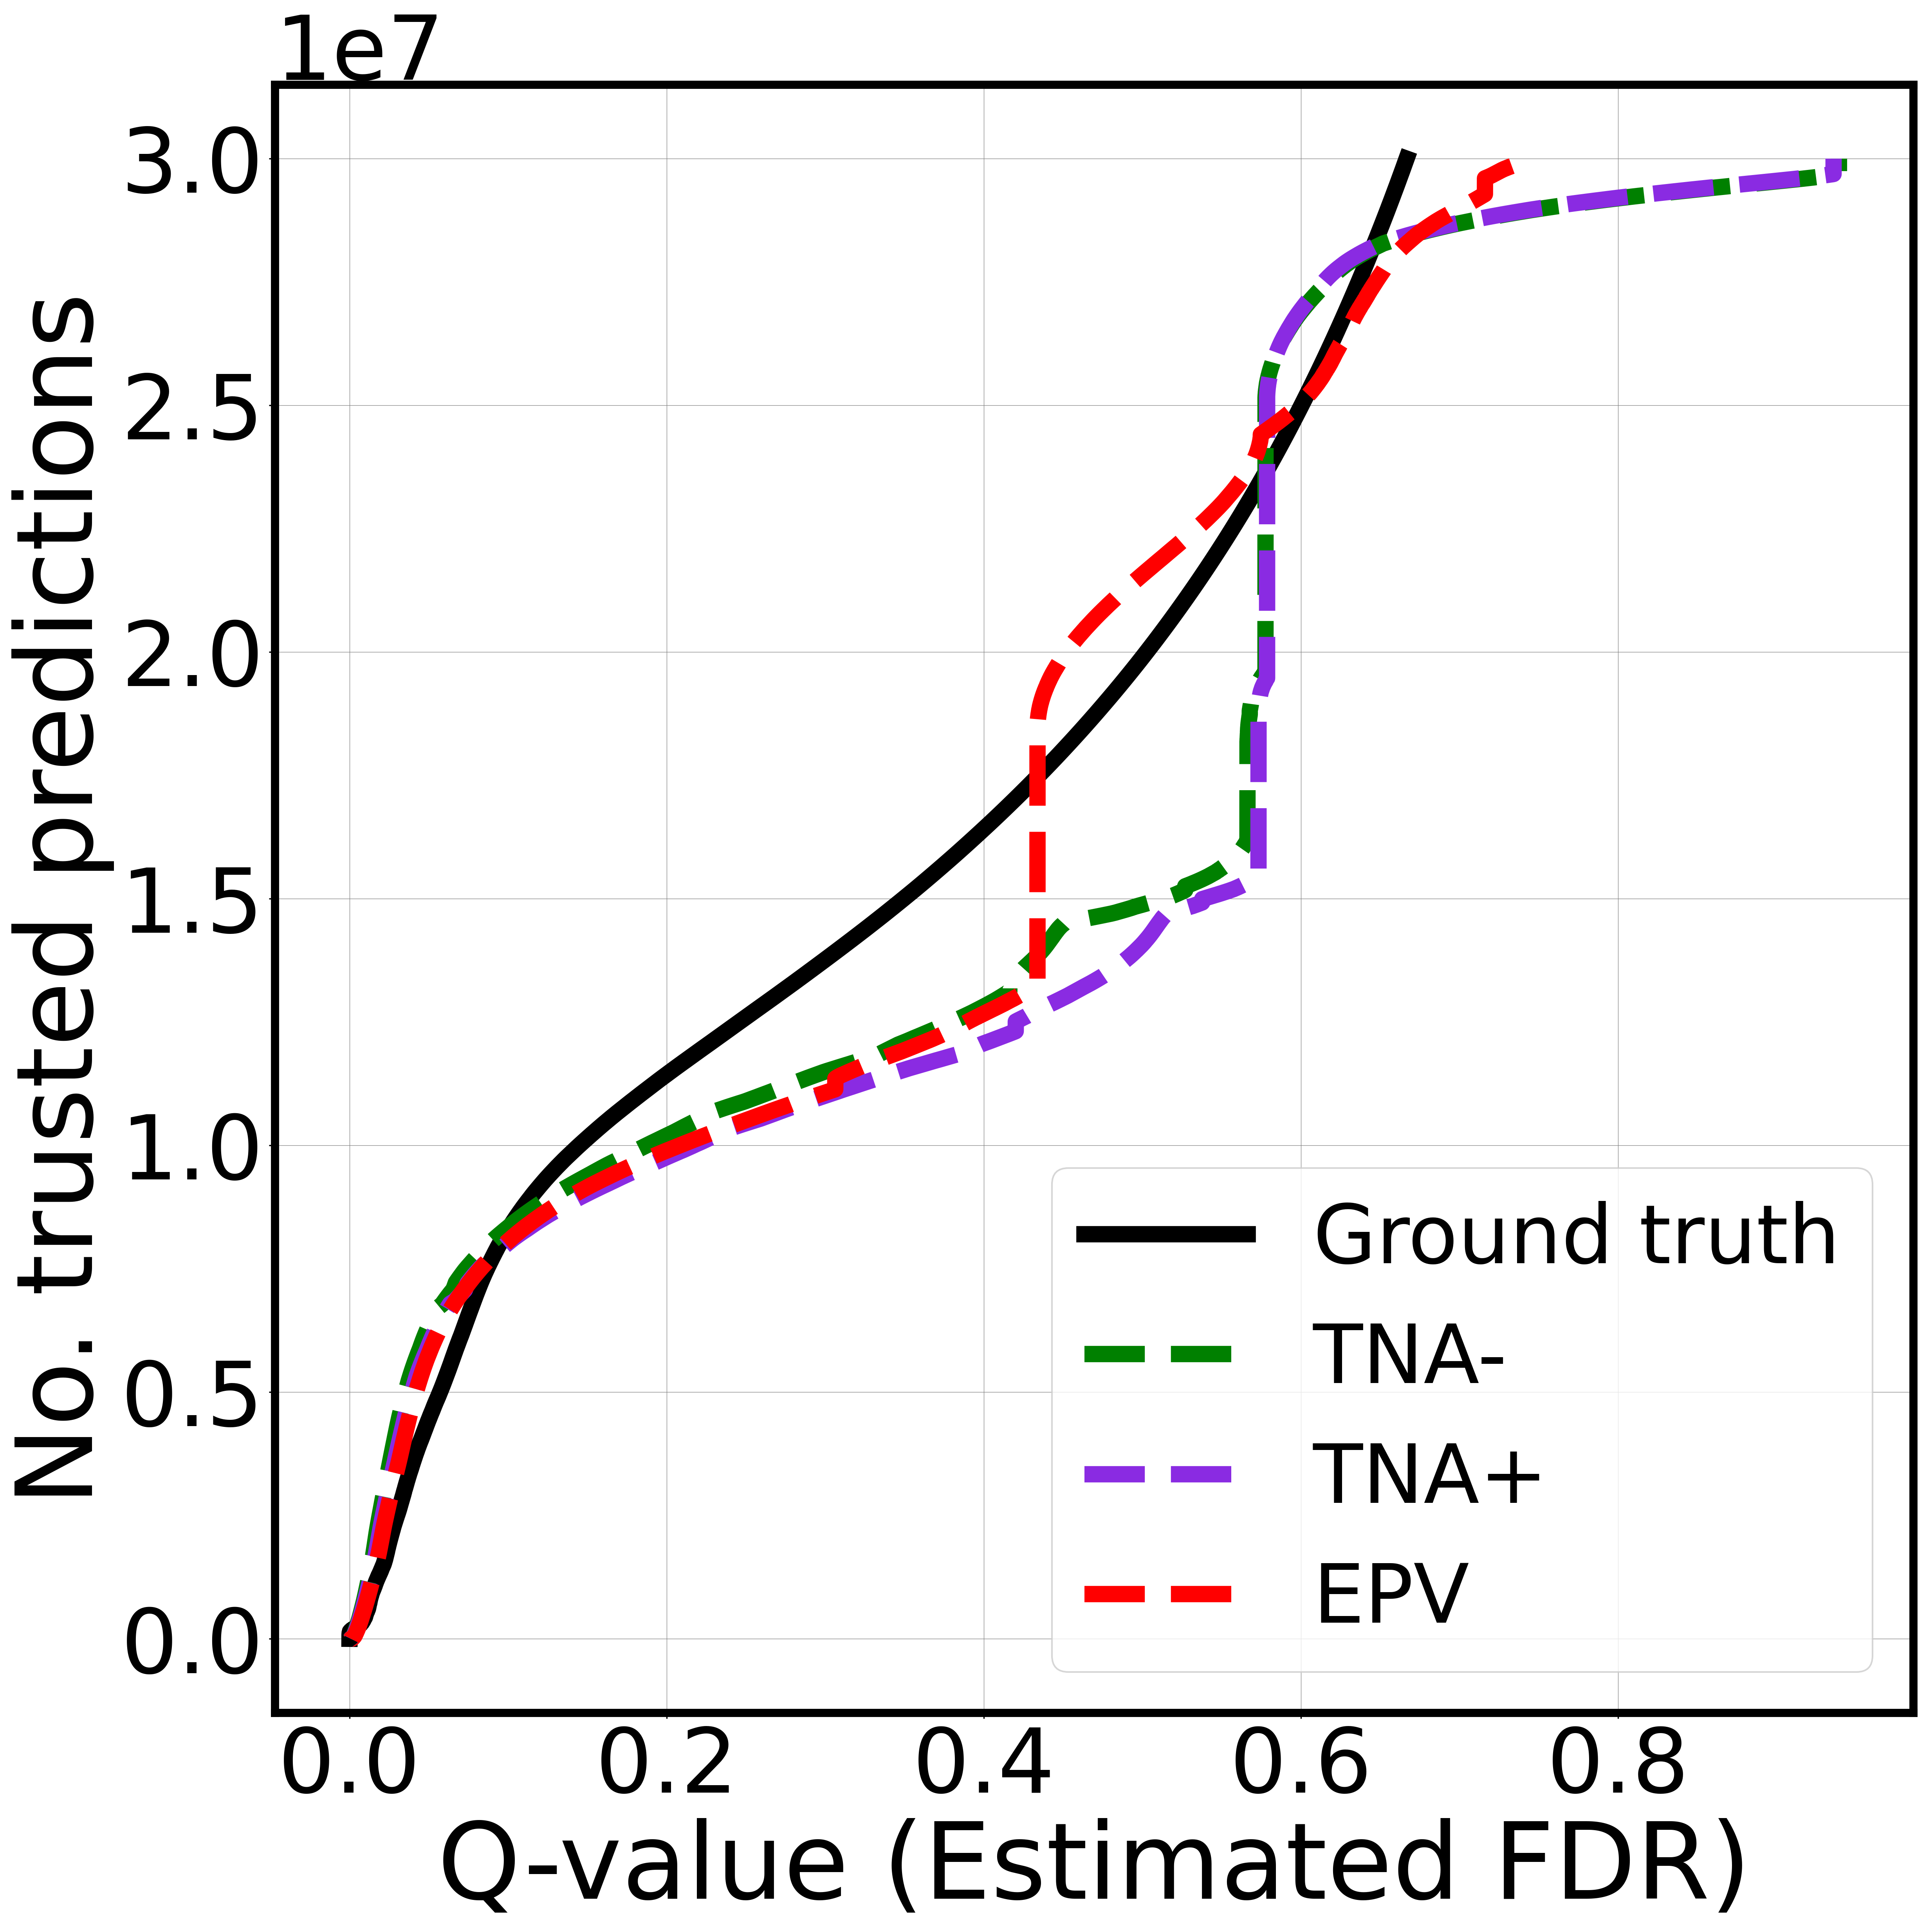
\includegraphics[width=0.225\linewidth, height=0.225\linewidth]{img/cnn_bcss_fdr_control.png} &
		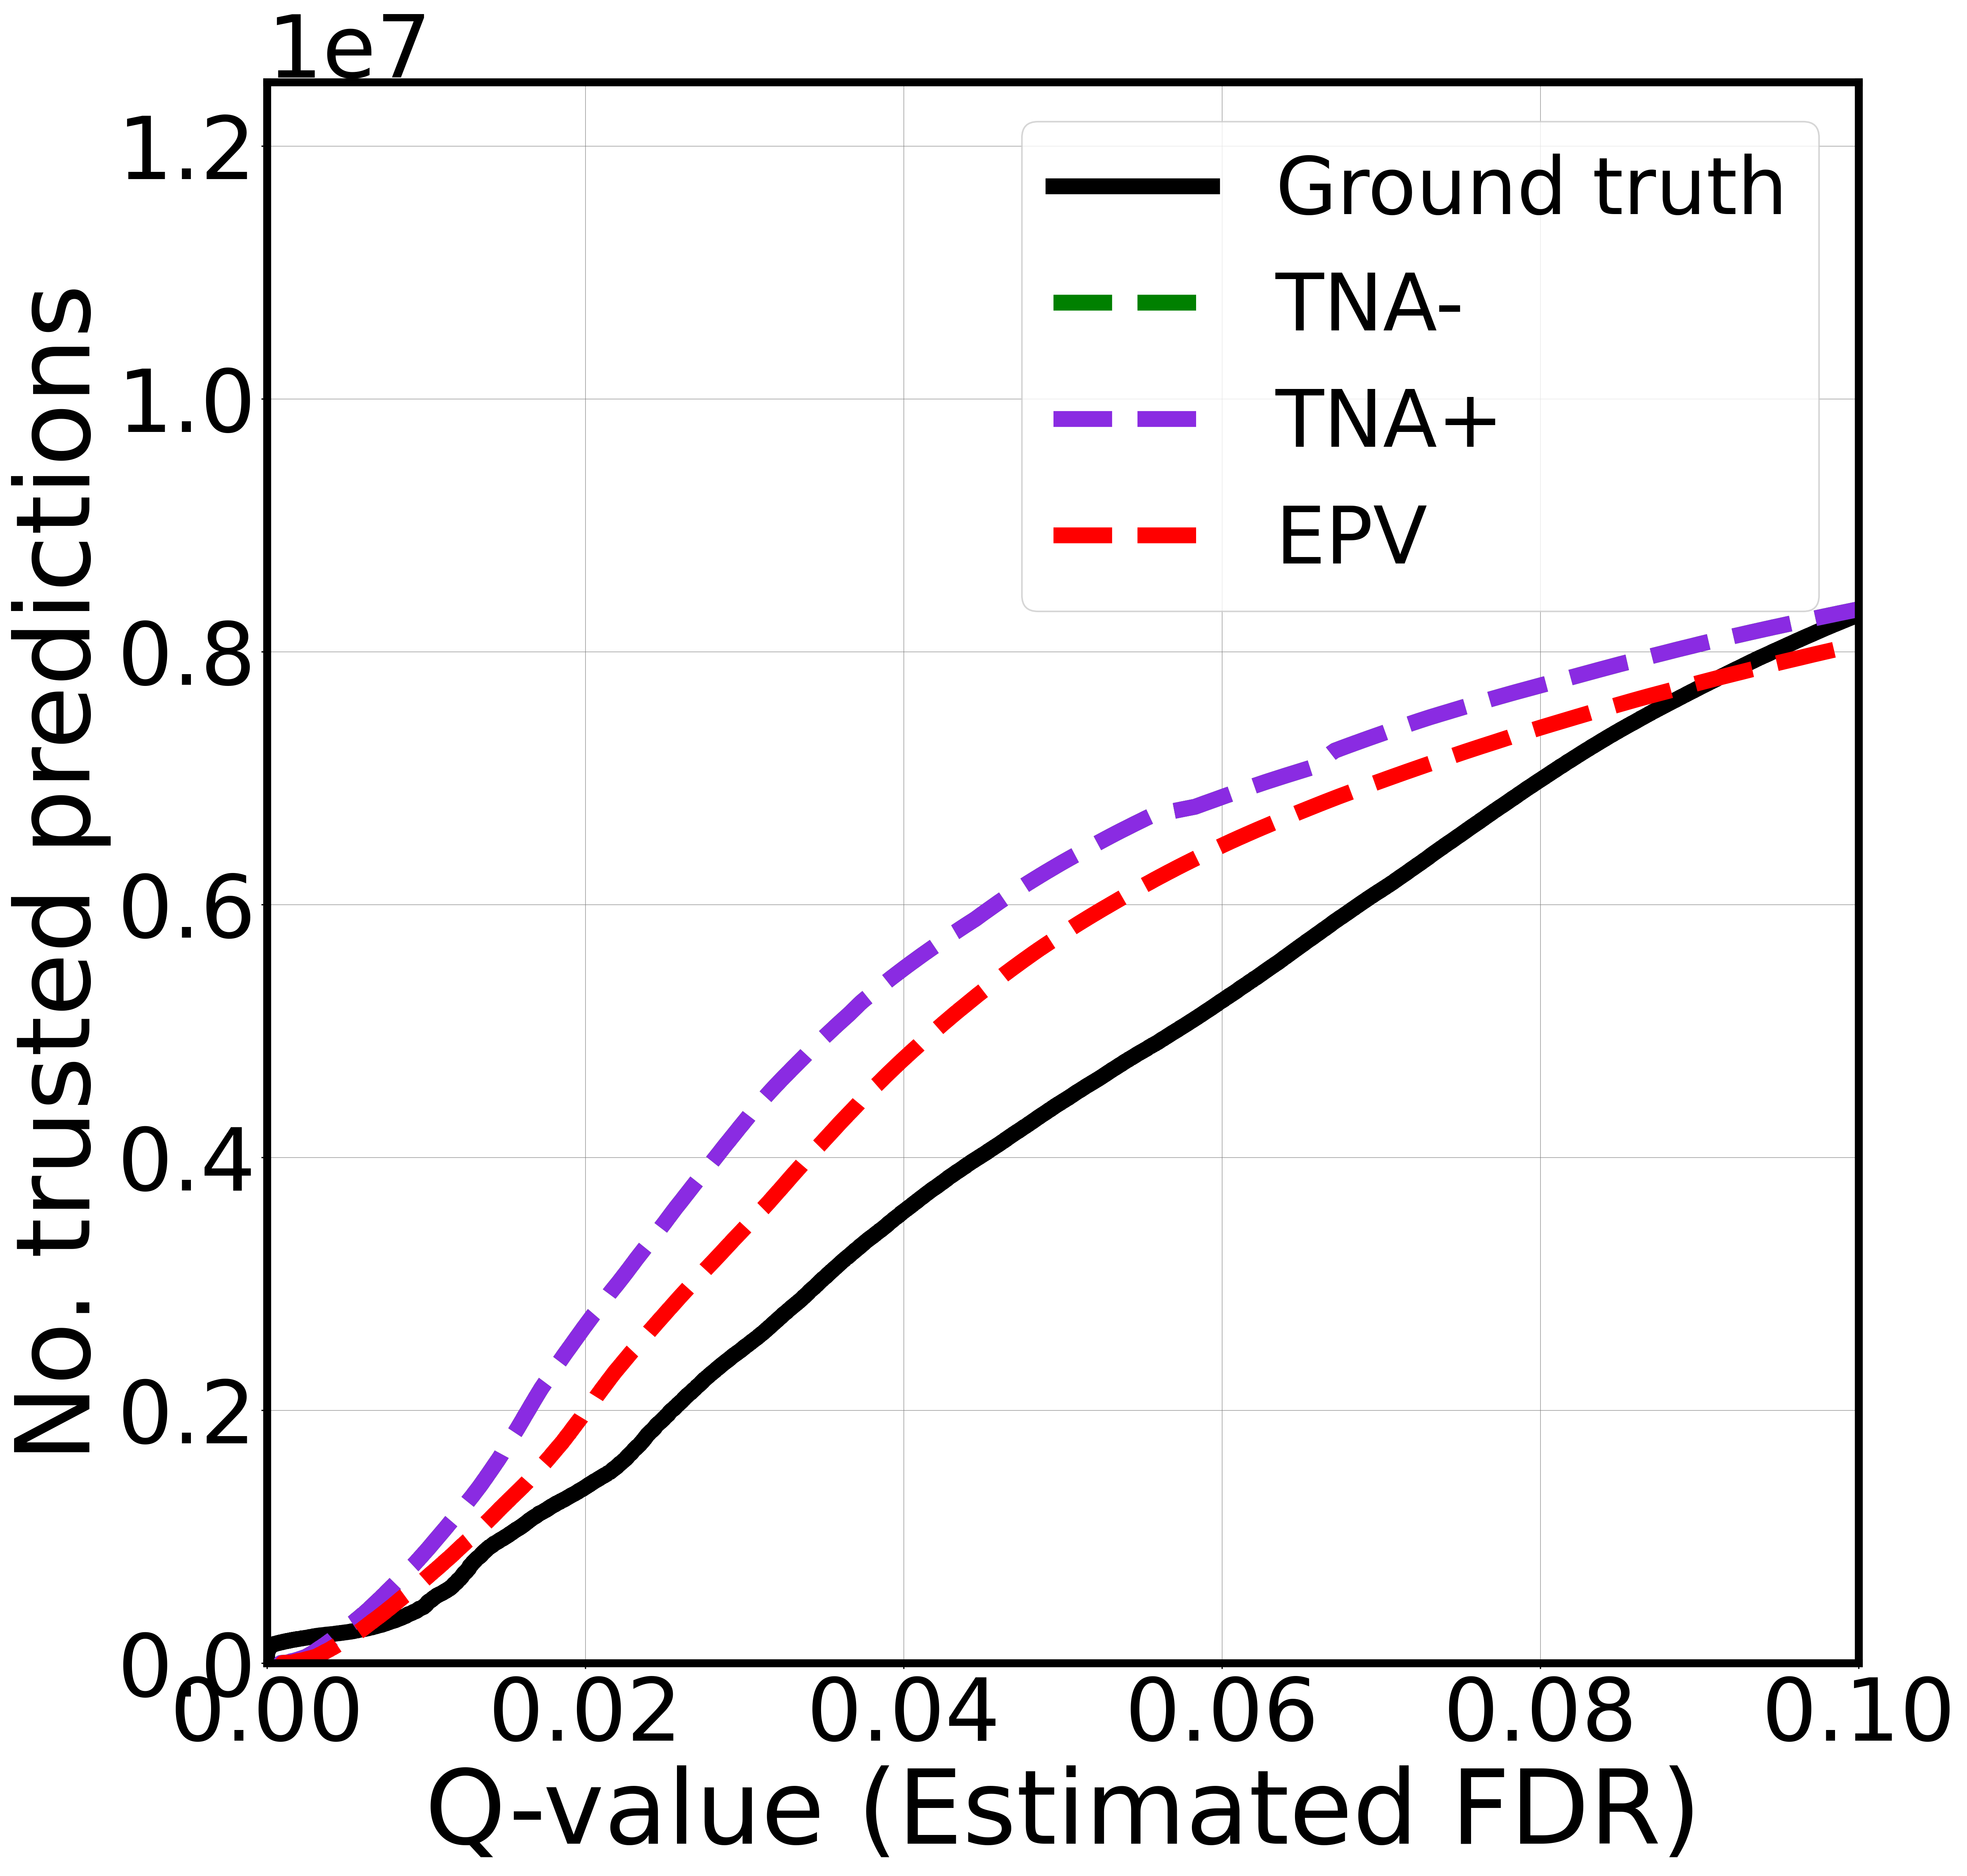
\includegraphics[width=0.225\linewidth, height=0.225\linewidth]{img/cnn_bcss_fdr_control_loc.png}  &
		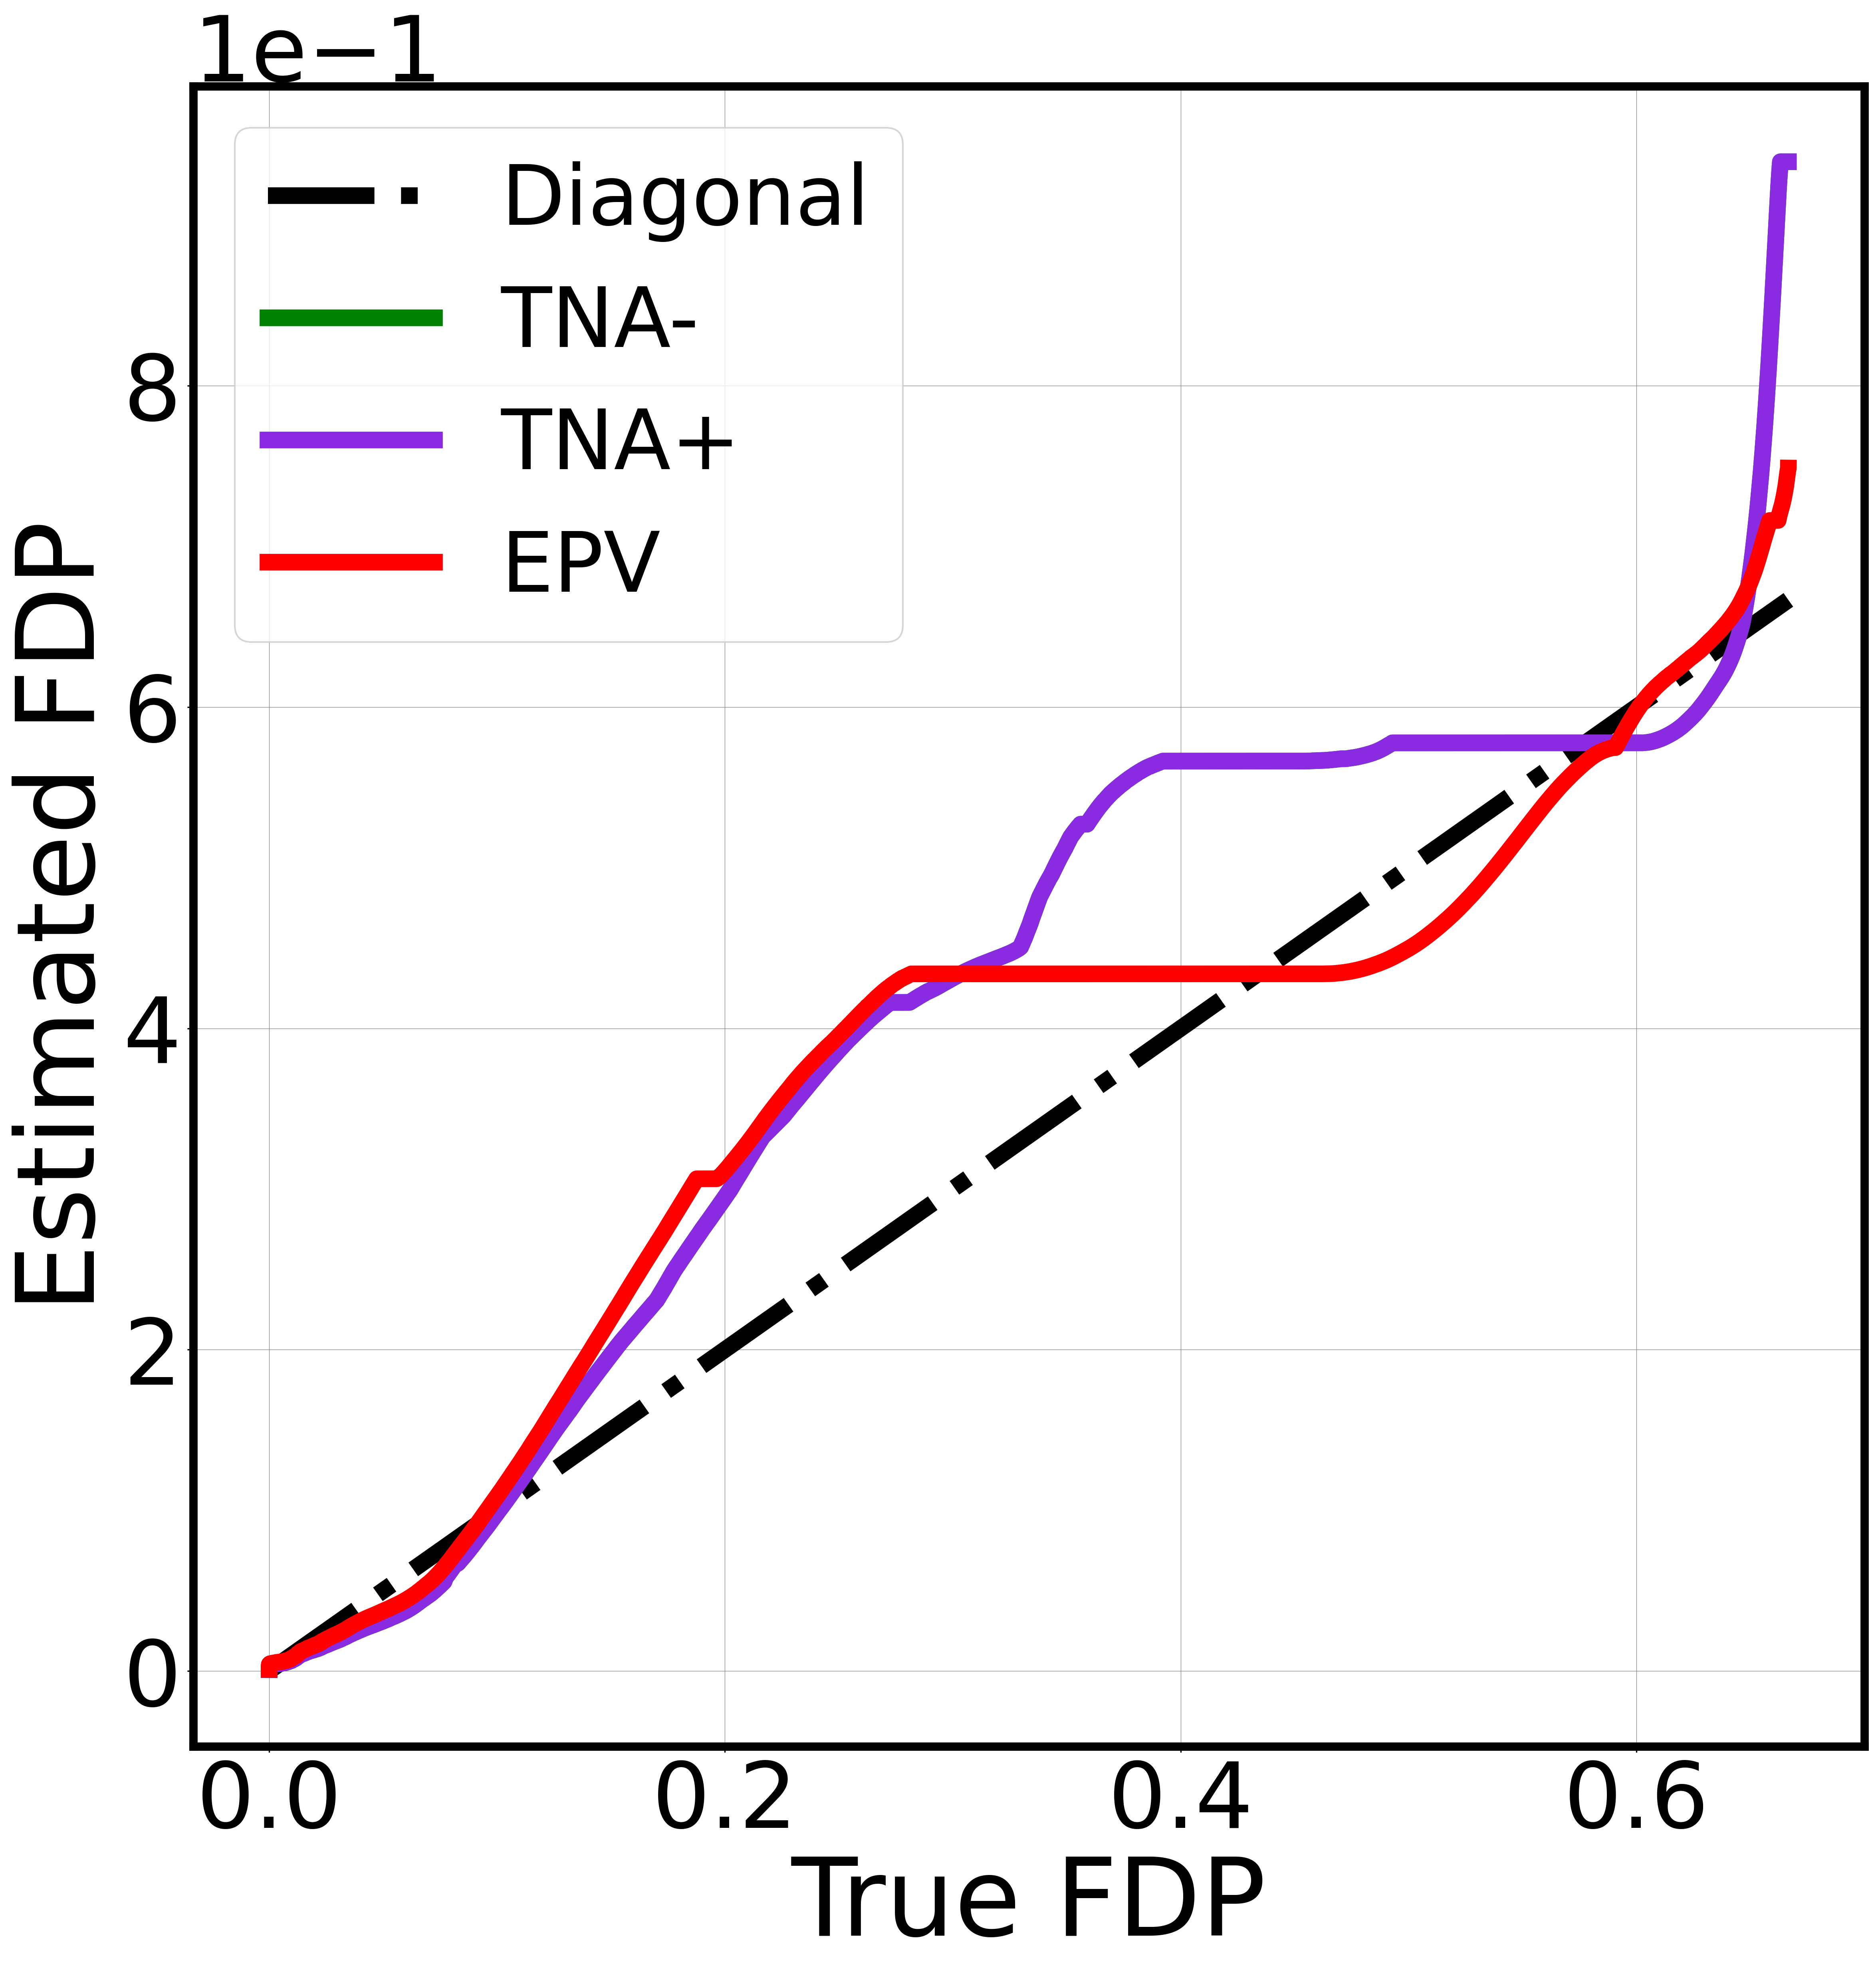
\includegraphics[width=0.225\linewidth, height=0.225\linewidth]{img/cnn_FDPscat_bcss.png}\\
		A & B & C & D
	\end{tabular}
	\caption{{\bf Performance evaluation of FDR controlling methods.}  See the caption of Figure \ref{fig:mnist_shfit} for plot descriptions.}
	\label{fig:ii}
\end{figure} 

The evaluation of the FDR controlling methods is shown in Figure \ref{fig:ii}-(iii). At first glance, the results suggest that this datasets is challenging and it  has a strong shift between the training and test data and/or the deep learning model has been profoundly overfit. The Q-Q plots of the EPVs and the TNA EPVs are far from being uniform (Fig. \ref{fig:ii}-(iii)-A). Overall, the BH control with standard and TNA EPVs is conservative (Fig. \ref{fig:ii}-(iii)-B), but it is slightly liberal over the critical range of q-values (0-0.1) (Fig. \ref{fig:ii}-(iii)-C). BH protocol seems to be more accurate with standard rather than with TNA EPVs. The FDR estimation error is significant (Fig. \ref{fig:ii}-(iii)-D). 

Next, we further analyzed the results by each class separately. We plotted the training and test positive and negative discriminative score distributions class-wise provided by the deep learning model (Fig. \ref{fig:BCSS-classwise} first row). The distribution plots show that the test scores are differently distributed from the train scores in all the classes. We also plotted the distribution of the adjusted scores of the negative test samples, adjusted by our TNA methods (green and purple lines in Fig. \ref{fig:BCSS-classwise}) in order to see how well they are aligned to the train null distribution.  In the case of the Stroma class, the mode of adjusted test scores (green and purple lines) move a bit closer to the one of the true train null distribution (X0, filled orange bars). However, their tails on the right hand side remain off. In the other two classes, the adjusted test scores align visibly better to the train null distribution (X0). The corresponding FDR curves are shown in the second row of Figure \ref{fig:BCSS-classwise}. Both the TNA- and the TNA+ methods worsen the results in the case of the Stroma class; however, they make the FDR control more accurate in the other two classes. This is mainly due to the fact that the Storey method provides better $\pi_0$ estimation using the TNA EPVs tha using the standard EPVs. 



\begin{figure}[h!]
	\centering	
	\begin{tabular}{ccc}
		Stroma & Tumor & Others \\
		\includegraphics[width=0.225\linewidth, height=0.225\linewidth]{img/bcss_0_neg_score_dist.png} &
		\includegraphics[width=0.225\linewidth, height=0.225\linewidth]{img/bcss_1_neg_score_dist.png} & 
		\includegraphics[width=0.225\linewidth, height=0.225\linewidth]{img/bcss_2_neg_score_dist.png} \\
		\includegraphics[width=0.225\linewidth, height=0.225\linewidth]{img/cnn_0th_bcss_class_fdr_control.png} &
		\includegraphics[width=0.225\linewidth, height=0.225\linewidth]{img/cnn_1st_bcss_class_fdr_control.png} & 
		\includegraphics[width=0.225\linewidth, height=0.225\linewidth]{img/cnn_2nd_bcss_class_fdr_control.png} \\
	\end{tabular}
	\caption{{\bf Classwise score distributions and FDR control in the BCSS dataset.}}
	\label{fig:BCSS-classwise}
\end{figure} 

\section{Conclusions}


In this study, we examined the effects of data shift on False Discovery Rate (FDR) control. In our opinion, the BH procedure with standard EPVs provides a very accurate FDR control in the absence of any data shift. Unfortunately, data shift is rather common in practice, and we demonstrated that the standard BH and the LTT methods are quite sensitive even to small data or class distribution shift. In this paper, we presented a simple, but robust method, called Test Null Adjustment (TNA), in order to mitigate the effect of the data shift on the FDR control. Our method operates in the space of prediction scores, thereby it is not affected by the curse-of-dimensionality problem, which often hinders methods that aim to mitigate data shift in the input feature space. The TNA method consists of two main steps. First, it approximates the null distribution among the scores of the test instances via certain statistics from the scores of the training instances. Second, it recalibrates the test scores so that the test and train null distributions would move closer to each other. TNA is fully data-driven, it does not rely on any theoretical assumptions or forms of the data. We have demonstrated in our experimental test with four biomedical datasets that TNA can successfully mitigate the bias caused by data shift; while, leaving the distributions intact in the absence of data shift. We note that, the handling of data shifts in practice is challenging, and unfortunately our method does not provide any theoretical guarantee that the FDR control with TNA EPVs becomes accurate, or conservatively or liberally biased without any additional assumptions; hence TNA is a heuristic in its general form.  

With this study, we also aim to emphasize and popularize the importance of accurate error control in any predictions in the biomedical domain. We have shown that the deviations in the simple Q-Q plots of the calculated vs. the theoretical p-values can be used to detect data shifts between the training and test data. Moreover, we also hope that the FDR control and plots with q-values will become a standard metric in performance evaluation for prediction systems in the biomedical domain.




%\printbibliography	 
%\bibliographystyle{plain}           % Style BST file.
\bibliographystyle{unsrt}           % Style BST file.
\bibliography{bibliography}

\section*{Author contributions}
\ifdefined\DOUBLEBLINDREVIEW
Omitted for double-blind peer-review.
\else
AKF concieved the idea and supervised the project,  AB worked out the methods and carried out experiments. AKF and AB wrote the manuscript.
\fi 
\section*{Data availability}
The data used in this study are secondary data obtained from publicly available sources. All data sources are properly cited within the manuscript. No new primary data were generated or analyzed in this research. For access to the datasets used, please refer to the original sources as indicated in the references section.

\section*{Additional information}
The authors declare no conflicts of interest.


\end{document}
